% Template for NAU "manuscript" style dissertation Mar 2023. Feel free to use with no guarantees or warranties.
\documentclass{book}
\usepackage[utf8]{inputenc}

\usepackage[bookmarks=true,
     pdfnewwindow=true,      % links in new window
     colorlinks=true,    % false: boxed links; true: colored links
     linkcolor=black,     % color of internal links; black to blue, 6/10/22 COC % black per NAU EDT 7/27/2022 COC
     citecolor=xlinkcolor,     % color of links to bibliography
     filecolor=xlinkcolor,  % color of file links
     urlcolor=xlinkcolor,      % color of external links
     final=true,
 ]{hyperref}

%for clickable footnote marks in author list to link to footnote affiliations
\newcounter{affilctr}
\newcommand{\affil}[1]{%
  \refstepcounter{affilctr}%
  % Put a superscript that links to the PDF destination:
  \textsuperscript{\hyperlink{affil:\theaffilctr}{\theaffilctr}}%
  % Now set the footnote text, with an internal PDF destination:
  \footnotetext[\value{affilctr}]{%
    % Shift the anchor up slightly so that the jump lands near the start:
    \raisebox{.5\baselineskip}{\pdfdest name {affil:\theaffilctr} xyz}%
    #1
  }%
}
% For reusing an already-declared affiliation:
\newcommand{\affilmark}[1]{%
  \textsuperscript{\hyperlink{affil:#1}{#1}}%
}

\usepackage[nointegrals]{wasysym}
\usepackage{siunitx}
\sisetup{
  separate-uncertainty = true,   % allows “±” style uncertainties
  round-mode = uncertainty,
  round-precision = 1,
  %table-align-uncertainty = true,
}
\usepackage[version=4]{mhchem}
\usepackage{mathtools} % loads amsmath also

\usepackage[letterpaper, portrait, margin=1in]{geometry}
\pagestyle{plain}
\raggedbottom  % CTU 22/12/12 get rid of space between paragraphs at end of chapters

\setcounter{secnumdepth}{3}

\usepackage{setspace}
\usepackage{lipsum}
\usepackage{float}
\usepackage{graphicx}
\usepackage{lscape}
\usepackage[printonlyused]{acronym}

\usepackage{listings} % to display code blocks
\usepackage{xcolor} % For defining custom colors
\usepackage{subcaption}
\usepackage{placeins}

% Define custom colors
\definecolor{codegreen}{rgb}{0,0.6,0}
\definecolor{codegray}{rgb}{0.5,0.5,0.5}
\definecolor{codepurple}{rgb}{0.58,0,0.82}
\definecolor{backcolour}{rgb}{0.95,0.95,0.92}

% Setup the code display style
\lstset{
    backgroundcolor=\color{backcolour},
    commentstyle=\color{codegreen},
    keywordstyle=\color{magenta},
    numberstyle=\tiny\color{codegray},
    stringstyle=\color{codepurple},
    basicstyle=\ttfamily\footnotesize,
    breakatwhitespace=false,
    breaklines=true,
    captionpos=b,
    keepspaces=true,
    numbers=left,
    numbersep=5pt,
    showspaces=false,
    showstringspaces=false,
    showtabs=false,
    tabsize=2
}
\usepackage{upgreek} % For upright Greek letters
\lstset{
  language=Go,
  extendedchars=true,
  literate=%
        {σ}{{\ensuremath{\upsigma}}}1 % Replace σ with \upsigma from upgreek package
        {Γ}{{\ensuremath{\Upgamma}}}1 % Replace Γ with \Upgamma from upgreek package
        {μ}{{\ensuremath{\upmu}}}1 % Replace μ with \upmu from upgreek package
        {³}{{\textsuperscript{3}}}1, % Replace ³ with superscript 3
}

% (Note to self: acronym package updated and broke this block)
% \makeatletter
% \newcommand*{\org@overidelabel}{}
% \let\org@overridelabel\@verridelabel
% \@ifpackagelater{acronym}{2015/03/21}{% v1.41
%   \renewcommand*{\@verridelabel}[1]{%
%     \@bsphack
%     \protected@write\@auxout{}{\string\AC@undonewlabel{#1@cref}}%
%     \org@overridelabel{#1}%
%     \@esphack
%   }%
% }{% older versions
%   \renewcommand*{\@verridelabel}[1]{%
%     \@bsphack
%     \protected@write\@auxout{}{\string\undonewlabel{#1@cref}}%
%     \org@overridelabel{#1}%
%     \@esphack
%   }%
% }
% \makeatother

\acrodef{ac}{Acronym}

% \usepackage{amssymb} % leftrightsquiggle, etc.
\usepackage{textcomp,gensymb} % degree, etc. CTU 10/20/22

\usepackage{xcolor}
\definecolor{xlinkcolor}{cmyk}{0,0,0,1} % per NAU EDT 7/27/2022 COC
\PassOptionsToPackage{hyphens}{url}

\usepackage[percent]{overpic}
\usepackage{color}

% \usepackage{cleveref}
% \crefformat{footnote}{#2\footnotemark[#1]#3}

\usepackage{url}
\usepackage[super,comma,sort&compress]{natbib}
\bibliographystyle{unsrtnat}  % Add different bib style .bst file if you'd like

% Ensure a nice space after comma in citation lists
\makeatletter
\renewcommand\NAT@citesuper[3]{%
 \ifNAT@swa
  \unskip\hspace{1pt}%
  \textsuperscript{#1}%
  \if*#3*\else\ (#3)\fi
 \else
  \textsuperscript{#1}%
  \if*#3*\else\ (#3)\fi
 \fi
 \endgroup
}
\renewcommand\NAT@sep{,\;}
\makeatother

\usepackage{enumitem}
\usepackage{makecell} % 12/27/2017 COC for multi-lined entries in tables
\usepackage{longtable} % spanning pages
\usepackage{booktabs}
\usepackage{multirow} % CJTU 12/15/22

% Wrapped figures and caption shenanigans 11/07/2022 CTU for inline figures
\usepackage[skip=5pt]{caption}
\DeclareCaptionFormat{boldtitle}
{%
    \textbf{#1#2} #3
}
\captionsetup{format=boldtitle,font={stretch=1.2}}
\usepackage{wrapfig} % for inline figures
\usepackage{etoolbox} % To fix misaligned wrapfigures
\BeforeBeginEnvironment{wrapfigure}{\setlength{\intextsep}{0pt}}
\BeforeBeginEnvironment{figure}{\setlength{\intextsep}{12.0pt plus 2.0pt minus 2.0pt}}

%Define custom units for siunitx package
\DeclareSIUnit{\sample}{Sa}
\DeclareSIUnit{\octave}{Oct}
\DeclareSIUnit{\dBm}{dBm}

% Aliases
\newcommand{\dissertationTitle}{COHERENTLY STIMULATED BRILLOUIN SPECTROSCOPY}
\newcommand{\degr}{$\degree$}
\newcommand{\hho}{H$_2$O}
\newcommand{\ohhho}{OH / \hho}

%%%%%%%%%%%%
%me-
\usepackage[immediate]{silence}
\WarningFilter[temp]{latex}{Command} % silence the warnings from sectsy "\underbar has changed" "\underline has changed"
\usepackage{sectsty} % 6/26/2022 COC: control style of sectioning (e.g., font size) <- original line
\DeactivateWarningFilters[temp] % So nothing unrelated gets silenced

\makeatletter % disable the runtime redefinitions
\let\SS@makeulinesect\relax
\let\SS@makeulinepartchap\relax
\makeatother
%-me

% \allsectionsfont{\sffamily}
\chapternumberfont{\large}
\chaptertitlefont{\large}
\chapterfont{\large}
\allsectionsfont{\large}
\subsectionfont{\large}
\subsubsectionfont{\normalsize}
\paragraphfont{\normalsize}
% \sectionnumberfont{\large}
% \sectiontitlefont{\large}

%%%%%%%%%%%%%%%%%
\usepackage{calc}

\newcounter{rownumber}%12/26/2017 COC
%\renewcommand{\therownumber}{\thetable.\arabic{rownumber}}
%\newcounter{rtaskno}
%\newcommand{\rtask}[1]{\refstepcounter{rtaskno}\label{#1}}
\newcommand{\rlabel}[1]{\refstepcounter{rownumber}\label{#1}}
\setcounter{rownumber}{-36}

\newcounter{tabfoot}
\newcommand{\flabel}[1]{\refstepcounter{tabfoot}\label{#1}}
\renewcommand{\thetabfoot}{\alph{tabfoot}}
\setcounter{tabfoot}{-6}

\newcommand{\fakechapter}[1]{%
  \par\refstepcounter{chapter}% Increase chapter counter
%   \chaptermark{#1}% Add chapter mark (header)
  \addcontentsline{toc}{chapter}{\protect\numberline{\thechapter}#1}% Add section to ToC
}
\newcommand{\fakesection}[1]{%
  \par\refstepcounter{section}% Increase section counter
%   \sectionmark{#1}% Add section mark (header)
  \addcontentsline{toc}{section}{\protect\numberline{\thesection}#1}% Add section to ToC
}

\usepackage[figuresleft]{rotating} % forces all clockwise rotation per NAU EDT guidelines
\usepackage{pdflscape}  % CTU 11/18/22 use for landscape figures/tables



%%%%%%%%%%%%%%%%%%%%%%%%%%%%%%%%%%%%%%%%%%%%%%%%%%%%%%%%%%%%%%%%%%%%%%%%%%%
\begin{document}

%%%%%%%%%%%%%%%%%%%%%%%%%%%%%%%%%%%%%%%%%%%%%%%%%%%%%%%%%%%%%%%%%%%%%%%%%%%
\frontmatter  % Roman numerals
\begingroup  % Begin start chapter on any page
\let\cleardoublepage\clearpage  % Allow chapters to start on even pages
\doublespacing
  \begin{centering}
\begin{large}
\begin{spacing}{1.8}

\vspace*{\baselineskip}

\dissertationTitle{}

\thispagestyle{empty} % 4/28/2022 COC -- no page number on first page

\vspace{\baselineskip}

By Joel N. Johnson

% \vspace{10mm}

A Dissertation

Submitted in Partial Fulfillment

of the Requirements for the Degree of

% \vspace{10mm}

Doctor of Philosophy

in Applied Physics and Materials Science

\vspace{\baselineskip}

Northern Arizona University

!Month YYYY!

\vspace{2\baselineskip}

%Approved:

Ryan O. Behunin, Ph.D., Co-Chair

John G. Gibbs, Ph.D., Co-Chair

Inès Montaño, Ph.D.

Jennifer S. Martinez, Ph.D.

\end{spacing}
\end{large}
\end{centering}

  \cleardoublepage
  \newpage
  \thispagestyle{empty}
  \null
  \newpage
  \phantomsection
\addcontentsline{toc}{chapter}{Abstract}

\begin{center}
    \large
    ABSTRACT

    \large
    \dissertationTitle{}

    \large
    \vspace{2mm}
    JOEL N. JOHNSON

\end{center}

% Abstract text max 350 words recommended
\noindent

This dissertation explores novel ways in which light and sound interact in optical waveguides to enable laser cooling of traveling-wave phonons and to enhance phonon spectroscopy. First, we establish how anti-Stokes Brillouin scattering can be harnessed to cool acoustic excitations in a continuous fiber, extending laser cooling concepts beyond discrete cavity optomechanical systems. By using a \ac{LCOF} filled with \ce{CS2}, we achieve significant reduction in the phonon population through spontaneous anti-Stokes processes. This demonstration marks the first instance of in-fiber traveling-wave phonon cooling without requiring nanophotonic resonators or specialized microstructures.

Second, we introduce a Coherently Stimulated Brillouin Spectrometer (\acs{CoBS}) that employs a four-wave mixing scheme—comprising pump, probe, driven Stokes, and observed signal fields—to dramatically improve sensitivity, especially for short, low-gain samples. By relaxing traditional phase-matching constraints, the CoBS approach enables sub-\SI{10}{\femto\watt} detection levels over millimeter- to centimeter-scale lengths. We validate its utility with measurements in both high- and low-gain media, opening new possibilities for ultrathin-film and microfluidic analyses.

Lastly, this dissertation investigates the theoretical and experimental conditions under which Brillouin-driven Raman-like modes might be observed. These “Brillouin-induced Raman” modes could provide a bridge between conventional Raman spectroscopy and the acousto-optic phenomena characteristic of traveling-wave phonons. While not yet fully realized, the groundwork here points to future avenues in which engineering the geometric and material properties of optical waveguides can yield both net phonon cooling and advanced hybrid phononic devices. Collectively, these results broaden our understanding of optomechanical coupling in fibers and pave the way for low-noise photonic systems, quantum acoustic memory elements, and highly sensitive, broadband spectroscopic tools.

  %%\include{pre/0-Copyright}

  \chapter*{}
\phantomsection

%\vspace*{.25\textheight}
\begin{center}
\textit{Science is temporal arbitrage; invest in it.}
\end{center}

  \chapter*{Dedication}
\phantomsection
\addcontentsline{toc}{chapter}{Dedication}

  \cleardoublepage
  \newpage
  \thispagestyle{empty}
  \null
  \newpage
  \chapter*{Acknowledgements}
\phantomsection
\addcontentsline{toc}{chapter}{Acknowledgements}

%\textit{Note: Manuscript-specific acknowledgements are found at the end of each corresponding chapter.}
%\section*{In Memoriam}
%\section*{Individuals and Groups}
%\section*{Funding}
%\section*{General Acknowledgements}

%Lauren

%Parents

%Gibbs: Live long and prosper, friend

%Research group: Gabe, V, Dylan, Dani

%friends: Josh, Tyler, Derek, others


%%%%%%%%%%%%%%%%%%%%%%%%%%%%%%%%%%%%%%%%%%%%%%%%%%%%%%%%%%%%%%%%%%%%%%%%%%
\singlespacing
\setcounter{tocdepth}{3} % depth of sections diplayed in table of contents
\phantomsection
\addcontentsline{toc}{chapter}{Table of Contents}
\renewcommand{\contentsname}{Table of Contents}
\tableofcontents
\doublespacing

%%%%%%%%%%%%%%%%%%%%%%%%%%%%%%%%%%%%%%%%%%%%%%%%%%%%%%%%%%%%%%%%%%%%%%%%%%
\clearpage
\phantomsection
\addcontentsline{toc}{chapter}{List of Tables}
\listoftables

%%%%%%%%%%%%%%%%%%%%%%%%%%%%%%%%%%%%%%%%%%%%%%%%%%%%%%%%%%%%%%%%%%%%%%%%%%
\clearpage
\phantomsection
\addcontentsline{toc}{chapter}{List of Figures}
\listoffigures
\endgroup  % End start chapter on any page
\doublespacing

%%%%%%%%%%%%%%%%%%%%%%%%%%%%%%%%%%%%%%%%%%%%%%%%%%%%%%%%%%%%%%%%%%%%%%%%%%

\chapter{List of Acronyms}
\label{chap:acronyms}

\begin{singlespace}
  \begin{acronym}
    \setlength{\parskip}{0pt}
    \acro{AC}{alternating current}
    \acro{AOM}{acousto-optic modulator}
    \acro{AMO}{atomic, molecular, and optical}
    \acro{BPF}{bandpass filter}
    \acro{BYU}{Brigham Young University}
    \acro{C}{Cooling metric}
    \acro{CARS}{Coherently stimulated Anti-Stokes Raman Scattering}
    \acro{CINT}{Center for Integrated Nanotechnologies}
    \acro{CoBS}{Coherently stimulated Brillouin Spectrometer}
    \acro{CW}{Continuous Wave}
    \acro{DC}{direct current}
    \acro{EDFA}{Erbium-Doped Fiber Amplifier}
    \acro{FBG}{fiber Bragg grating}
    \acro{FP}{fiber port}
    \acro{FWHM}{full-width half-max}
    \acro{GLAD}{glancing angle deposition}
    \acro{IM}{fiber-optic intensity modulator}
    \acro{LANL}{Los Alamos National Laboratory}
    \acro{LCOF}{liquid-core optical fiber}
    \acro{LO}{local oscillator}
    \acro{ORNL}{Oak Ridge National Laboratory}
    \acro{PC}{polarization controller}
    \acro{PCF}{photonic crystal fiber}
    \acro{PBS}{polarizing beam splitter}
    \acro{PVD}{physical vapor deposition}
    \acro{RBW}{resolution bandwidth}
    \acro{RF}{radio frequency}
    \acro{RFSA}{radio-frequency spectrum analyzer}
    \acro{SNL}{Sandia National Laboratory}
    \acro{SBS}{Stimulated Brillouin Scattering}
    \acro{SMF-28}{single mode fiber 28}
    \acro{SNR}{signal-to-noise ratio}
    \acro{UHNA3}{Ultra High Numerical Aperture 3}
    \acro{UHNA7}{Ultra High Numerical Aperture 7}
    \acro{VOA}{Variable Optical Attenuator}
    \acro{WGM}{whispering-gallery-mode}
  \end{acronym}
\end{singlespace}


%%%%%%%%%%%%%%%%%%%% INTRO & METHODS %%%%%%%%%%%%%%%%%%%%%%%%%%%%%%%%%%%%%

\mainmatter  % Regular numbers
\chapter{Introduction}
\label{ch:Introduction}
\acresetall

%TOO SELF INTERESTED! State facts
%The work presented in this document details my efforts toward achieving a result for which my time and available resources would prove too limited to accomplish in full. It is my great hope that a dear future reader may someday be inspired to take up where I left off and realize the result that I have been chasing for these years. No physical principle disallows the demonstration of this result, only practical challenges stand in its way.

%The physics involved in this research effort primarily lies in the field of optomechanics, however it veers at times into the related domains of nonlinear optics and nanoscience. I have in fact developed a great love for each of these fields and it was my romantic goal to unite them that originally led me to pursue this work. In this introductory chapter I present the foundational topics and concepts that I employ in later chapters.

Optomechanics is the study of light-matter interactions; it is the study of how the intangible (light) can affect change in the tangible (matter) and vice versa. Injecting light into a material under specific conditions allows for an exchange of energy to occur between the light and the mechanical oscillations of the material which changes the mechanical energy of the material. This interaction can be controlled to deposit or withdraw mechanical energy into/from a system and thus leave the system in a more, or less, mechanically energetic state respectively. The same interaction can also be harnessed for passive observation of material properties. Mechanical systems from bulk to atomic scales can be probed and characterized with light by retrieving the inelastically scattered light resulting from interaction with the material. This retrieved light contains embedded information about the energy exchange that occurred, which, when considered as part of a population of scattering events, reveals natural resonances of a mechanical system.

Optomechanics comprises a broad range of phenomena involving the interaction of optical and mechanical systems, from basic photothermal absorption to more complex nonlinear processes. Here I offer a brief overview of notable optomechanical phenomena then devote the remainder of this chapter to a more detailed description of the specific interactions that play a role in my research. Photothermal absorption is the process by which light is absorbed by a material, leading to an increase in temperature of the material and consequent changes in the material's dimensions (thermal expansion) or refractive index (thermo-optic effect). This effect has applications in optical switches\cite{}, actuators\cite{}, and sensors\cite{}. Photothermal therapy in medicine is an emerging application of this effect, where light is used to target and heat specific areas, causing localized damage to diseased tissue\cite{}. This technique becomes especially effective when combined with nanoparticle-enhanced absorption, allowing for dramatically increased absorption in ultra-localized zones within the body.

Light scattering, in its many forms, is also an optomechanical process as it involves the interaction of an optical field with the fluctuation, motion, or vibration of matter. Rayleigh scattering, perhaps the most well-known example, is the elastic scattering of light by particles much smaller than the wavelength of the incident light, leading to scattering in possibly a new direction but without a change in wavelength. It is responsible for the blue color of the sky because the efficiency of Rayleigh scattering is inversely proportional to the fourth power of the wavelength ($\lambda$) of the light ($\frac{1}{\lambda^{4}}$) and so shorter (blue) wavelengths are scattered much more than longer (red) wavelengths by the molecules in the atmosphere.\cite{rayleigh1871light}

Raman scattering is the interaction of light with vibrational and rotational modes within a material (often molecular), resulting in scattered light with frequencies that are shifted from the incident light. This inelastically scattered light provides insights into the material's molecular structure and properties. Raman scattering is widely used in chemical and material science for identifying chemical compounds, analyzing molecular structures, and studying molecular dynamics. It finds application in the characterization of pharmaceuticals\cite{}, monitoring changes in biological tissues for medical diagnostics\cite{}, and investigation of stress and temperature distributions in engineering materials\cite{}, among others\cite{}.

Brillouin scattering, around which much of my work is centered, is the scattering of light with acoustic phonons or coherent traveling density waves in a material, resulting in scattered light with a frequency that is slightly shifted from the incident light. This inelastically scattered light reveals mechanical properties of the material such as its bulk and elastic moduli. This phenomenon is used in materials science to measure elastic properties and viscoelasticity of materials\cite{}, in fiber optic sensing to monitor temperature and strain over large distances\cite{}, and in physics to study phase transitions and mechanical properties of crystals, liquids, and gases\cite{}.

Rayleigh-wing scattering is the broad, smooth extension of the Rayleigh scattering spectrum that results from interactions with low-frequency excitations in a material, providing insights into dynamic processes like rotational and translational diffusion of molecules that make up a material. This scattering is particularly useful in studying the dynamics of complex fluids, gases, and soft materials, where it can reveal information about molecular orientation, diffusion rates, and interactions within the medium. Applications include the analysis of atmospheric phenomena\cite{}, characterization of liquid crystals\cite{}, and investigations into the properties of polymers and biological materials\cite{}, aiding in the understanding of their behavior at the molecular level.

Figure \ref{fig:Introduction:scattering-domains} shows the relative domains of typical frequency shifts for Rayleigh, Rayleigh-wing, Brillouin, and Raman scattering. Rayleigh-wing scattering is broad and shares part of its domain with Brillouin scattering. This makes sense because for any given molecule and within the timescale that it occurs, diffusive translational motion can be thought of as indistinguishable from motion caused by traveling density waves that host brillouin scattering. In this way, Rayleigh-wing scattering represents a sporadic distribution of fleeting, localized Brillouin scattering. Of course, the difference between incoherent diffusion of molecules and coherently traveling acoustic modes within a material is an important distinction. However, this thought experiment offers a perspective for bridging the gap between Rayleigh-wing and Brillouin scattering and for understanding their common frequency domains. Moreover, it serves as a reminder of the rich continuum of material behavior and responses that affect light scattering as opposed to the distinct categories we ascribe for convenience. This is a core concept of my work.%Boyd 9.6 works out general theory of Brillouin and Rayleigh scattering!

% This makes sense, as the [random and incoherent] translational motion of molecules as they [continuously] diffuse [according to the laws of thermodynamics and as described by statistical mechanics] can be thought of, within the timescale that this motion occurs, as indistinguishable from [translational motion as caused by coherent] traveling density waves which host brillouin scattering.

\begin{figure}[t] % here (h), at the top (t), at the bottom (b), or on a separate page for floats (p), in that preference order
\centering
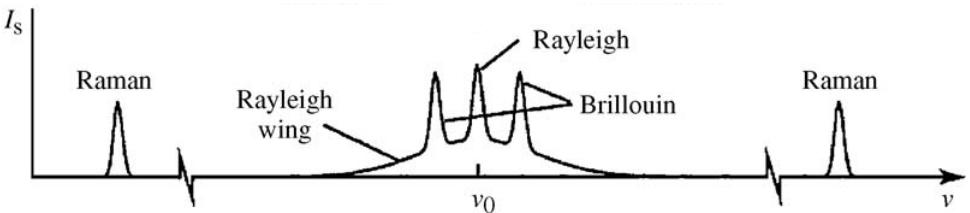
\includegraphics[width=0.75\linewidth]{figs/1-Intro/Boyd scattering frequency shift domains.png}
\caption{Relative domains of typical frequency shifts for Rayleigh, Rayleigh-wing, Brillouin, and Raman scattering.}
\label{fig:Introduction:scattering-domains}
\end{figure}

Returning to other optomechanical phenomena beyond scattering processes, the momentum of photons can exert forces on objects, leading to phenomena like radiation pressure, optical tweezing, and optical trapping. These effects are widely used in manipulating microscopic particles\cite{}, biological cells\cite{}, and atoms\cite{}, enabling studies of single molecules\cite{}, cold atoms\cite{}, and quantum computing elements\cite{}.

The final category of optomechanical interactions I will note here is that of nonlinear optical phenomena. Second harmonic generation, parametric oscillation, and four-wave mixing all feature the interaction between light and material nonlinearities that lead to the generation of new light frequencies.\cite{boyd2020nonlinear} The Kerr effect is the change in the refractive index of a material in response to an applied electric field, which can be induced optically with sufficient intensities of light. In general, nonlinear optical responses of materials are often only accessible with the use of high intensity laser light. This is emphasized by the fact that the field of nonlinear optics can be traced back to the discovery of second-harmonic generation in 1961\cite{franken1961generation}, just one year after the first demonstration of the laser by American physicist Theodor Maiman.\cite{maiman1960stimulated} These nonlinear effects provide the foundation for a range of technologies, including high-speed optical communication systems\cite{}, frequency converters\cite{}, and lasers for materials processing\cite{}.

Also included within nonlinear optical phenomena is electrostriction. Electrostriction is a reversible material deformation induced by an electric field, which can be generated by light in electro-optic materials. This effect is quadratic, scaling with the square of the applied electric field, and hence a nonlinear optical effect. At sufficiently high intensities, electrostrictive forces serve to enhance Brillouin scattering whereby the scattered light electrostrictively reinforces the acoustic wave that caused its scattering, leading to a nonlinear positive feedback loop known as \ac{SBS}. Photostriction is a related phenomenon that occurs when light absorption causes a change in the lattice structure of a material, leading to mechanical strain. It combines photovoltaic and piezoelectric effects and can be seen as an optically induced strain. These effects are utilized in designing optical modulators\cite{}, tunable photonic devices\cite{}, and smart materials that respond to light\cite{}.

In the remainder of this chapter I further describe the specific optomechanical phenomena that pertain to the research presented in this document: Brillouin scattering, electrostriction as it pertains to the \ac{SBS} process, and Raman scattering.


%%%%%%%%%%%%%%%%%%%%%%%%%%%%%%%%%%%
\section{Light Scattering}
\label{sec:Introduction:Light-Scattering}
Light scattering involves the redirection of light as a result of interactions with the constituent particles or molecules within a material medium. In every case, light scattering occurs because of variations in the material's optical properties. To understand why, envision a material with completely uniform particles---spatially and temporally consistent, or in other words, perfectly homogeneous. Figure \ref{fig:Introduction:homogeneous-material-no-scatter} shows an incident optical plane wave encountering a segment of such a material, denoted $\delta z$, containing a volume element $\delta V_{1}$. For any given incident wavelength $\lambda$ and any non-zero scattering angle $\theta$ at volume $\delta V_{1}$, there exists a corresponding volume element $\delta V_{2}$, located a distance $\frac{\lambda}{2\sin\theta}$ apart, which scatters light at the same angle $\theta$. The scattered waves from $\delta V_{1}$ and $\delta V_{2}$ would be out of phase by $\frac{\lambda}{2}$, leading to perfect destructive interference and no resultant scattered field. Thus, to achieve observable scattering, the material must possess inhomogeneities, allowing for variations in the optical properties between neighboring volumes. Fortunately, perfect homogeneity is not characteristic of real materials; all matter undergoes thermodynamic fluctuations at any temperature above absolute zero, and quantum fluctuations are inherent even at the ground state.

I now begin with a theoretical description of spontaneous light scattering as a result of thermodynamic fluctuations, presented in Boyd Nonlinear Optics.\cite{boyd2020nonlinear} This foundation will serve as a framework for understanding light scattering as specifically resulting from pressure variations (Brillouin scattering) as opposed to density variations (Rayleigh scattering). Later I will treat the case of higher-intensity \ac{SBS}. Ultimately I will build upon this theoretical basis to derive the coupled-wave equations of \ac{CABS}, a novel instrument which underpins many of my results. Let us build a theoretical description of light scattering considering thermodynamic fluctuations as the origin of the scattering process.

\begin{figure}[t] % here (h), at the top (t), at the bottom (b), or on a separate page for floats (p), in that preference order
\centering
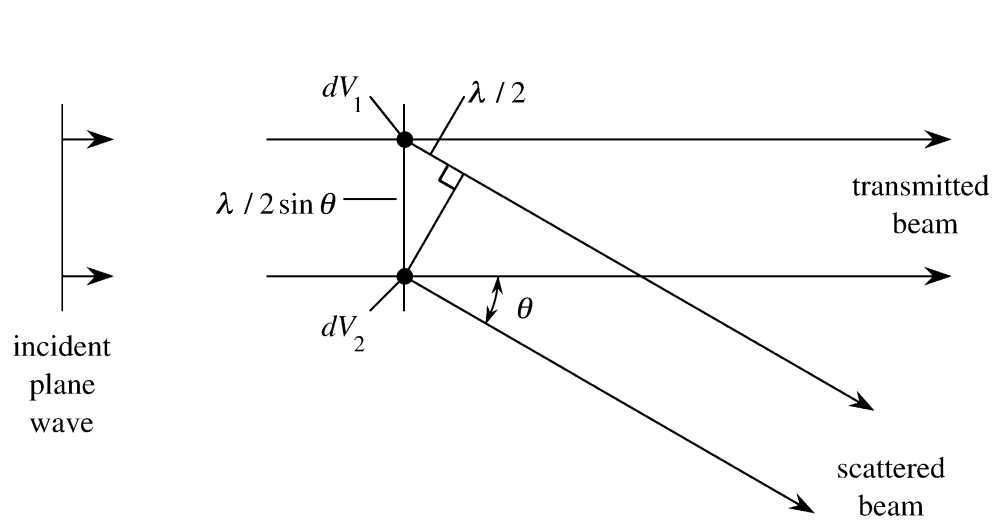
\includegraphics[width=0.75\linewidth]{figs/1-Intro/Boyd homogeneous material no scatter.png}
\caption{}
\label{fig:Introduction:homogeneous-material-no-scatter}
\end{figure}

\section{Spontaneous Brillouin Scattering}
\label{sec:Introduction:Spontaneous-Brillouin}
\lipsum[1]

\section{Stimulated Brillouin Scattering}
\label{sec:Introduction:Stimulated}
\lipsum[1]

\section{Phase-matching}
\label{sec:Introduction:Phase-matching}
\lipsum[1]

\section{Brillouin Gain of Materials}
\label{subsec:Introduction:Gain}
\lipsum[1]

\section{Raman Scattering}
\label{sec:Introduction:Raman}
\lipsum[1]

\section{Raman-like Brillouin Modes}
\label{sec:Introduction:Raman-like}
\lipsum[1]


%\chapter{Foundational Experimental Techniques and Instrumentation}
\label{ch:Experimental}
\acresetall

This is an inline citation, \cite{boyd2020nonlinear}. This is a parenthetical citation \citep{boyd2020nonlinear}. This is a figure reference (Figure \ref{fig:Introduction:scattering-domains}). This is a section reference \S\ref{sec:Introduction:Spontaneous-Brillouin}. This is a chapter reference with chapter spelled out: \autoref{ch:Cooling}. This is an acronym definition \ac{AGU}. This is the second time I use the acronym in this section \ac{AGU}. This is if I want to spell out the full acronym again \acf{AGU}. Define new acronyms in the acronyms.tex file.

%--------------------------------------------------------------------%

\section{Photonic Experimental Techniques}
\label{sec:Experimental:Experimental Techniques}


\subsection{Control of Light in Photonic Systems}
\label{subsec:Experimental:Techniques:Control}


\subsection{Photonic Devices and Diagrams}
\label{subsec:Experimental:Techniques:Diagrams}


\subsection{Selection and Isolation of Signals}
\label{subsec:Experimental:Techniques:Signals}


\subsection{Heterodyne Detection and the Local Oscillator}
\label{subsec:Experimental:Techniques:Heterodyne}


\subsection{Optical Loss in a Photonic Systems}
\label{subsec:Experimental:Techniques:Loss}


\subsection{Free Space Optics and Beam Alignment}
\label{subsec:Experimental:Techniques:Alignment}


\subsection{Specialized Optical Fibers}
\label{subsec:Experimental:Techniques:Fibers}

%--------------------------------------------------------------------%

\section{Optical Instrumentation}
\label{sec:Experimental:Optical Instrumentation}

%--------------------------------------------------------------------%

\section{Electronic Instrumentation}
\label{sec:Experimental:Electronic Instrumentation}

%--------------------------------------------------------------------%

\section{Noise and Background Handling}
\label{sec:Experimental:Noise}

%--------------------------------------------------------------------%

\section{Custom Software}
\label{sec:Experimental:Software}


\subsection{Description of Python Script for CABS Data Collection}
\label{subsec:Experimental:Software:Python}


\subsection{Description of Plotting Data in Go Program}
\label{subsec:Experimental:Software:Go}


%%%%%%%%%%%%%%%%%%% CHAPTERS %%%%%%%%%%%%%%%%%%%%%%%%%%%%%%%%%%%%%%%%%%%%%

\setcounter{rownumber}{0}
\chapter{Manuscript I: Laser cooling of traveling wave phonons in an optical fiber}
\label{ch:Cooling}
\acresetall

%--------------------------------------------------------------------%

\section{Abstract}
\label{sec:Cooling:Abstract}

%--------------------------------------------------------------------%

\section{Optomechanical Cooling and Heating}
\label{sec:Cooling:Cooling-Heating}

%--------------------------------------------------------------------%

\section{Cooling Platform: \texorpdfstring{$CS_{2}$}{CS2}-Liquid Core Optical Fiber}
\label{sec:Cooling:Platform}


\subsection{Optomechanical Properties}
\label{subsec:Cooling:Platform:Properties}


\subsection{Fabrication}
\label{subsec:Cooling:Platform:Fabrication}


\subsection{Fabrication Iterative Refinement}
\label{subsec:Cooling:Platform:Refinement}

%--------------------------------------------------------------------%

\section{Intention of the Pump-Probe Experiment}
\label{sec:Cooling:Intention}

%--------------------------------------------------------------------%

\section{Experimental Setup}
\label{sec:Cooling:Setup}


\subsection{Main Experiment}
\label{subsec:Cooling:Setup:Main}


\subsection{Pump-Probe Experiment}
\label{subsec:Cooling:Setup:Pump-Probe}

%--------------------------------------------------------------------%

\section{Results}
\label{sec:Cooling:Results}


\subsection{Main Experiment Results}
\label{subsec:Cooling:Results:Main}


\subsection{Pump-Probe Experiment Results}
\label{subsec:Cooling:Results:Pump-Probe}

%--------------------------------------------------------------------%

\section{Discussion}
\label{sec:Cooling:Discussion}


\subsection{Application to Ground State Cooling}
\label{subsec:Cooling:Discussion:Ground-State}


\subsection{Standardized Cooling Metric}
\label{subsec:Cooling:Discussion:Metric}


\subsection{Tapered chalcogenide Photonic Crystal Fiber: Max Plank Results}
\label{subsec:Cooling:Discussion:Max-Plank}


\setcounter{rownumber}{0}
\chapter{A Coherently Stimulated Phonon Spectrometer}
\label{ch:CoBS}
\acresetall

\hfill

\textit{This chapter presents a preview of an article in-prep for publication. Neither the author nor the publisher are responsible for any errors or omissions in any future publication derived from this version of the manuscript.}

\doublespacing

\section{Abstract}
We present a novel coherently stimulated Brillouin spectrometer utilizing a detuned pump-probe design that exploits a relaxation of phase-matching requirements at small lengths, enabling room-temperature traveling-wave phonon spectroscopy at the micrometer scale with sub-\SI{10}{\femto\watt} sensitivity. This approach overcomes the limitations of traditional stimulated Brillouin techniques, particularly regarding phase-matching constraints and spatial resolution. We validated my instrument’s sensitivity with \SI{1}{\centi\meter} of \ac{UHNA3} fiber and \SI{100}{\micro\meter} of bulk carbon disulfide liquid, demonstrating its capability to measure Brillouin scattering in materials with low Brillouin gain or, with particular advantage, small effective lengths. This advancement opens new possibilities for nanometer-scale Brillouin spectroscopy and the development of nano-acousto-optic devices.

\section{Introduction}
\label{sec:Introduction}

Brillouin scattering, the inelastic interaction between light and acoustic phonons, is a fundamental phenomenon for probing the mechanical and structural properties of materials at microscopic scales. In spontaneous Brillouin scattering, thermally excited acoustic phonons scatter incident light, causing frequency shifts that reveal information about the material’s elastic properties and acoustic modes \cite{boyd2020nonlinear}. However, the weak signal inherent to spontaneous Brillouin scattering often demands long acquisition times and limits spatial resolution, posing challenges for high‐resolution material characterization.

\ac{SBS} uses intense optical fields to amplify the acoustic wave through a nonlinear optical process \cite{chiao1964stimulated}. In \ac{SBS}, a strong pump laser interacts with a counter‐propagating Stokes wave in the medium, generating acoustic phonons via electrostriction. As the phonon population grows, it further amplifies the Stokes wave. In turn, that amplified Stokes wave interferes with the pump and reinforces the acoustic field, creating a positive feedback loop that drives exponential amplification. This mechanism enables more efficient excitation and detection of acoustic phonons and underpins numerous applications in optical signal processing, sensing, and high‐resolution spectroscopy including mechanobiology \cite{eggleton2013inducing, fotiadi2023brillouin, kobyakov2009stimulated, ippen1972stimulated, speziale2014brillouin, palombo2019brillouin, dil1982brillouin, eggleton2019brillouin, prevedel2019brillouin, conrad2019mechanical}.

%this whole paragraph needs to be rewritten to set up the phase matching restricitons that continue to pose a challenge\cite{yu2024chip} as a thing that my method solves.
However, conventional \ac{SBS} techniques struggle with short samples or materials of inherently low Brillouin gain and strict phase matching requirements continue to pose a challenge. \cite{rakich2012giant, gyger2020observation, yu2024chip}. Because the Stokes amplitude depends on the product of the Brillouin gain coefficient, pump power, and interaction length, small volumes often yield weak signals unless extremely high optical powers are used. Moreover, while backward \ac{SBS} sends the scattered wave in the opposite direction of the pump, parasitic reflections and pump leakage can still obscure the Stokes signal, demanding careful optical isolation and sometimes elaborate filtering. These constraints make it difficult to measure thin films and micro‐ and nanoscale devices, particularly if high optical intensities risk damaging sensitive samples. As a result, standard \ac{SBS} approaches are not easily adapted to sub‐centimeter lengths or low‐gain media, prompting the need for new methods that maintain high sensitivity in short interaction regions.

To overcome these challenges, researchers have explored various approaches \cite{shin2013tailorable, van2015interaction, kittlaus2016large, djadaojee2020stimulated, gusev2018advances, gerakis2011coherent}. Techniques based on optical cavities increase the effective interaction length, but require precise alignment and are sensitive to environmental fluctuations \cite{pant2011cavity}. Forward Brillouin scattering methods, such as those demonstrated by Kittlaus et al. \cite{kittlaus2017chip}, offer relaxed phase‐matching conditions but introduce increased modal complexity. Meanwhile, coherent probe beam amplification can boost sensitivity, yet it can introduce additional noise and complexity because phase noise in laser sources can cause significant gain fluctuations \cite{shlomovits2015effect}.

Here, wedemonstrate a detuned pump–probe design that relaxes the usual phase‐matching constraints at short lengths. This approach offers a new route to measure traveling‐wave phonons in sub‐centimeter or even micrometer‐scale samples at room temperature with unprecedented sensitivity. We demonstrate the capabilities of my instrument by measuring Brillouin scattering in \SI{1}{\centi\meter} of \ac{UHNA3} fiber and \SI{100}{\micro\meter} of bulk carbon disulfide (\ce{CS2}) liquid. These measurements highlight the instrument’s ability to characterize materials with low Brillouin gain or small effective lengths.

The development of this coherently stimulated Brillouin spectrometer opens new avenues for nanometer‐scale Brillouin spectroscopy and advances the characterization and design of nano‐acousto‐optic devices. It holds promise for pushing research in material science, photonics, and sensing technologies toward higher spatial resolution and sensitivity, marking a significant step toward practical, room‐temperature Brillouin‐based spectroscopy and sensing solutions.

\section{Theoretical Framework}
\label{Theoretical Framework}

\subsection{Coherently Stimulated Four-Wave Brillouin Scattering}
\label{Theoretical Framework:Coherently stimulated five-wave Brillouin scattering}

\begin{figure*}[t]
  \centering
  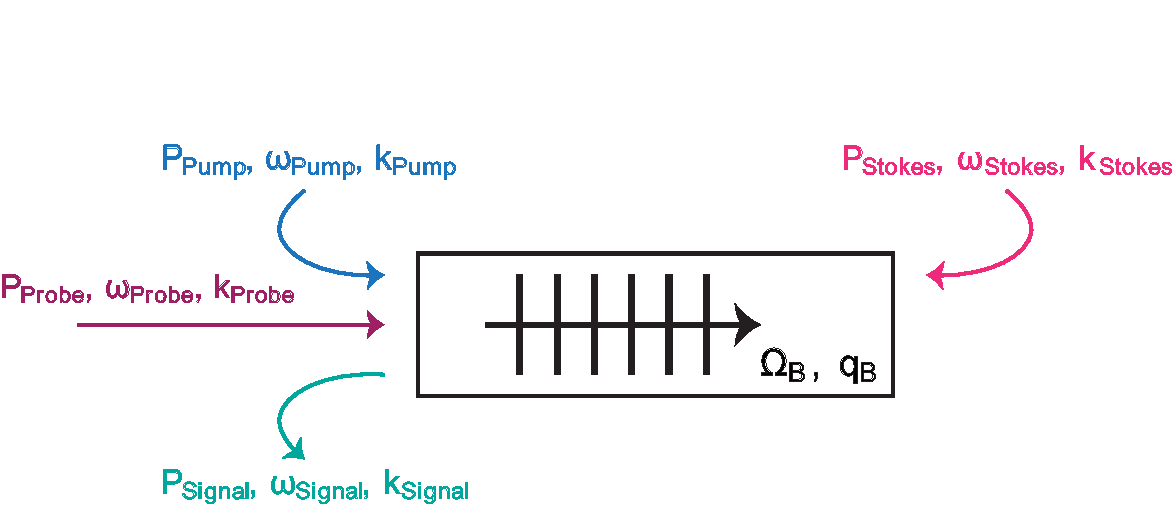
\includegraphics[width=\textwidth]{figs/4-CoBS/4-Wave-Brillouin-Scattering.pdf}
  \caption{Illustration of 4-Wave Brillouin Scattering.}
  \label{fig:4-Wave-Brillouin-Scattering}
\end{figure*}

Traditional \ac{SBS} is a three-wave mixing process in which incident pump laser light of frequency \(\omega_{\mathrm{Pump}}\) inelastically scatters from a traveling-wave phonon of frequency \(\Omega\) to produce light that is frequency-shifted by the phonon frequency. In the Stokes process the phonon is retreating from the incident laser light and the scattered light is shifted down in frequency (\(\omega_{\mathrm{Stokes}} = \omega_{\mathrm{Pump}} - \Omega\)). Spatial overlap of the backscattered light with the incident laser light allows for interference of the two optical fields to produce a frequency at the difference of the two (\(\omega_{\mathrm{Pump}} - \omega_{\mathrm{Stokes}}\)). Since this difference frequency is exactly equal to the frequency of the acoustic field \(\Omega\), the beating of the incident pump light with the backscattered Stokes light produces an electrostrictive reinforcement of the acoustic wave. This driving of the acoustic wave in turn increases the scattering rate of the incident pump light, producing a positive feedback process and an exponential increase of the amplitude of the backscattered Stokes wave.

Figure~\ref{fig:4-Wave-Brillouin-Scattering} illustrates coherently stimulated four-wave Brillouin scattering for the Stokes process. We introduce a strong, controlled external Stokes wave of frequency \(\omega_{\mathrm{Stokes}}\) that drives electrostrictive reinforcement of the acoustic field in the medium. The backscattered Stokes light is normally collected in an \ac{SBS} process, but the external Stokes laser overwhelms it. To resolve this, weinject light of a distinct frequency \(\omega_{\mathrm{Probe}}\) from an additional external laser which copropagates with the Pump and backscatters in the medium from the strongly driven acoustic field. This produces backscattered Signal light to be collected (\(\omega_{\mathrm{Signal}} = \omega_{\mathrm{Probe}} - \Omega\)) which is spectrally distinct from the high-powered Stokes laser light.

To describe this interaction and characterize the performance of the instrument, wederive the coupled-wave equations for the four-wave mixing process in Appendix~\ref{Appendix:Coupled-Wave Equations}. These equations describe the relationship between the optical fields and the acoustic field in the material and result in the following expression for the scattered power of the backscattered signal,
\\
\begin{equation}
  P_{Sig} = \frac{1}{4}(G_{B}L)^{2}P_{P}P_{S}P_{Pr}sinc^{2}\left(\frac{\Delta kL}{2}\right),
  \label{Eq:Theoretical Framework:Scattered Power}
\end{equation}
\\
where \(P_P\), \(P_S\), and \(P_Pr\) are the powers of the pump, Stokes, and probe lasers, respectively. \(G_B\) is the effective Brillouin gain, given by
\\
\begin{equation}
  G_{B} = \frac{g_{0}}{A_{eff}}\frac{\left(\frac{\Gamma_{B}}{2}\right)^{2}}{(\Omega - \Omega_{B})^{2} + \left(\frac{\Gamma_{B}}{2}\right)^{2}},
  \label{Eq:Effective Brillouin Gain}
\end{equation}
\\
with the on-resonance gain factor of the material given by
\\
\begin{equation}
  g_{0} = \frac{\gamma_{e}^{2}\omega^{2}}{nvc^{3}\rho_{0}\Gamma_{B}}.
\end{equation}
\\
Here, \(\gamma_e\) is the electrostrictive constant, \(\omega\) is the pump frequency, \(n\) is the refractive index of the material, \(v\) is the sound speed of the material, \(c\) is the speed of light, \(\rho_0\) is the mean density of the material, and \(\Gamma_B\) is the Brillouin linewidth, or phonon dissipation rate, of the material. In Equation~\ref{Eq:Effective Brillouin Gain}, \(\Omega_B\) is the resonant Brillouin frequency of the material, \(A_{Eff}\) is the effective area of the material, \(\Delta k\) is the wavevector mismatch between the optical fields, to be discussed next, and \(L\) is the effective length of the material.


\subsection{Phase Matching Relaxation}
\label{Theoretical Framework: Phase matching relaxation}
In all nonlinear optical processes, efficiency is maximized when phase matching conditions are satisfied. A frequency mismatch (energy unconservation) or a wavevector mismatch (momentum unconservation) each result in drastically reduced efficiency of a given process.\cite{maker1962effects} This can be seen by Equation~\ref{Eq:Theoretical Framework:Scattered Power}, where the wavevector mismatch, \(\Delta k\), is contained within a \(\mathrm{sinc^2}\) function. This \(\mathrm{sinc^2}\) term thereby defines the phase matching bandwidth of the system, notably scaling with effective interaction length \(L\).

We apply this wavevector mismatch allowance to the pump and probe waves (\(\Delta k = k_{\mathrm{Pump}} - k_{\mathrm{Probe}}\)) so that the backscattered signal is different than the applied Stokes wave. This choice allows for selection of the signal and rejection of the Stokes with a bandpass filter. Expressed in terms of wavelengths, this gives
\\
\begin{equation}
  \Delta k = \frac{4\pi n\Delta\lambda}{\lambda_{Pump}\lambda_{Probe}} \approx \frac{4\pi n\Delta\lambda}{\lambda_{Pump}^{2}}.
\end{equation}
\\
We can apply this to the phasematching bandwidth term to find the fraction of maximum scattered power, \(\Phi\), that can be expected for a given interaction length, \(L\), and phase mismatch \(\Delta\lambda\) between the pump and probe,
\\
\begin{equation}
  \Phi \equiv sinc^{2}\left(\frac{2\pi n\Delta\lambda L}{\lambda_{Pump}^{2}}\right).
  \label{Eq:Phi}
\end{equation}
\\
Using this expression for \(\Phi\), wesee that for an effective length of \SI{1}{\meter}, a wavelength mismatch of only \SI{0.6}{\pico\meter} from a typical wavelength of \SI{1.55}{\micro\meter} pump light in \ac{UHNA3} fiber drops the scattered power to half of the maximum. However, for shorter effective lengths the wavevector mismatch becomes more forgiving; a \SI{36}{\pico\meter} mismatch preserves 82.5\% of the maximum signal for a length of \SI{1}{\centi\meter} under identical conditions. This separation translates to about \SI{4.5}{\giga\hertz}, providing enough spectral separation for the backscattered signal to be isolated from the applied Stokes light.

Furthermore, for decreasing lengths, Equation~\ref{Eq:Phi} predicts an increase in the fraction of maximum signal produced, given equivalent pump--probe detuning, as the \(\mathrm{sinc^2}\) function is sampled closer to its peak center. Alternatively, as length decreases, the probe may be further detuned from the pump and still achieve the same fraction of the maximum signal as for longer lengths, perhaps offering a slight advantage in noise reduction. It should be noted that the scattered power, as given by Equation~\ref{Eq:Theoretical Framework:Scattered Power}, scales with the square of the effective length. Thus, while smaller lengths allow for the ability to capture a larger fraction of this maximum scattered power, the actual amount of scattered power decreases dramatically as length decreases.

\section{Methods}\label{Methods}
\subsection{Instrument Design}
\label{Methods:Instrument Design}

\begin{figure*}[htbp]
\centering
\vspace{-20mm}
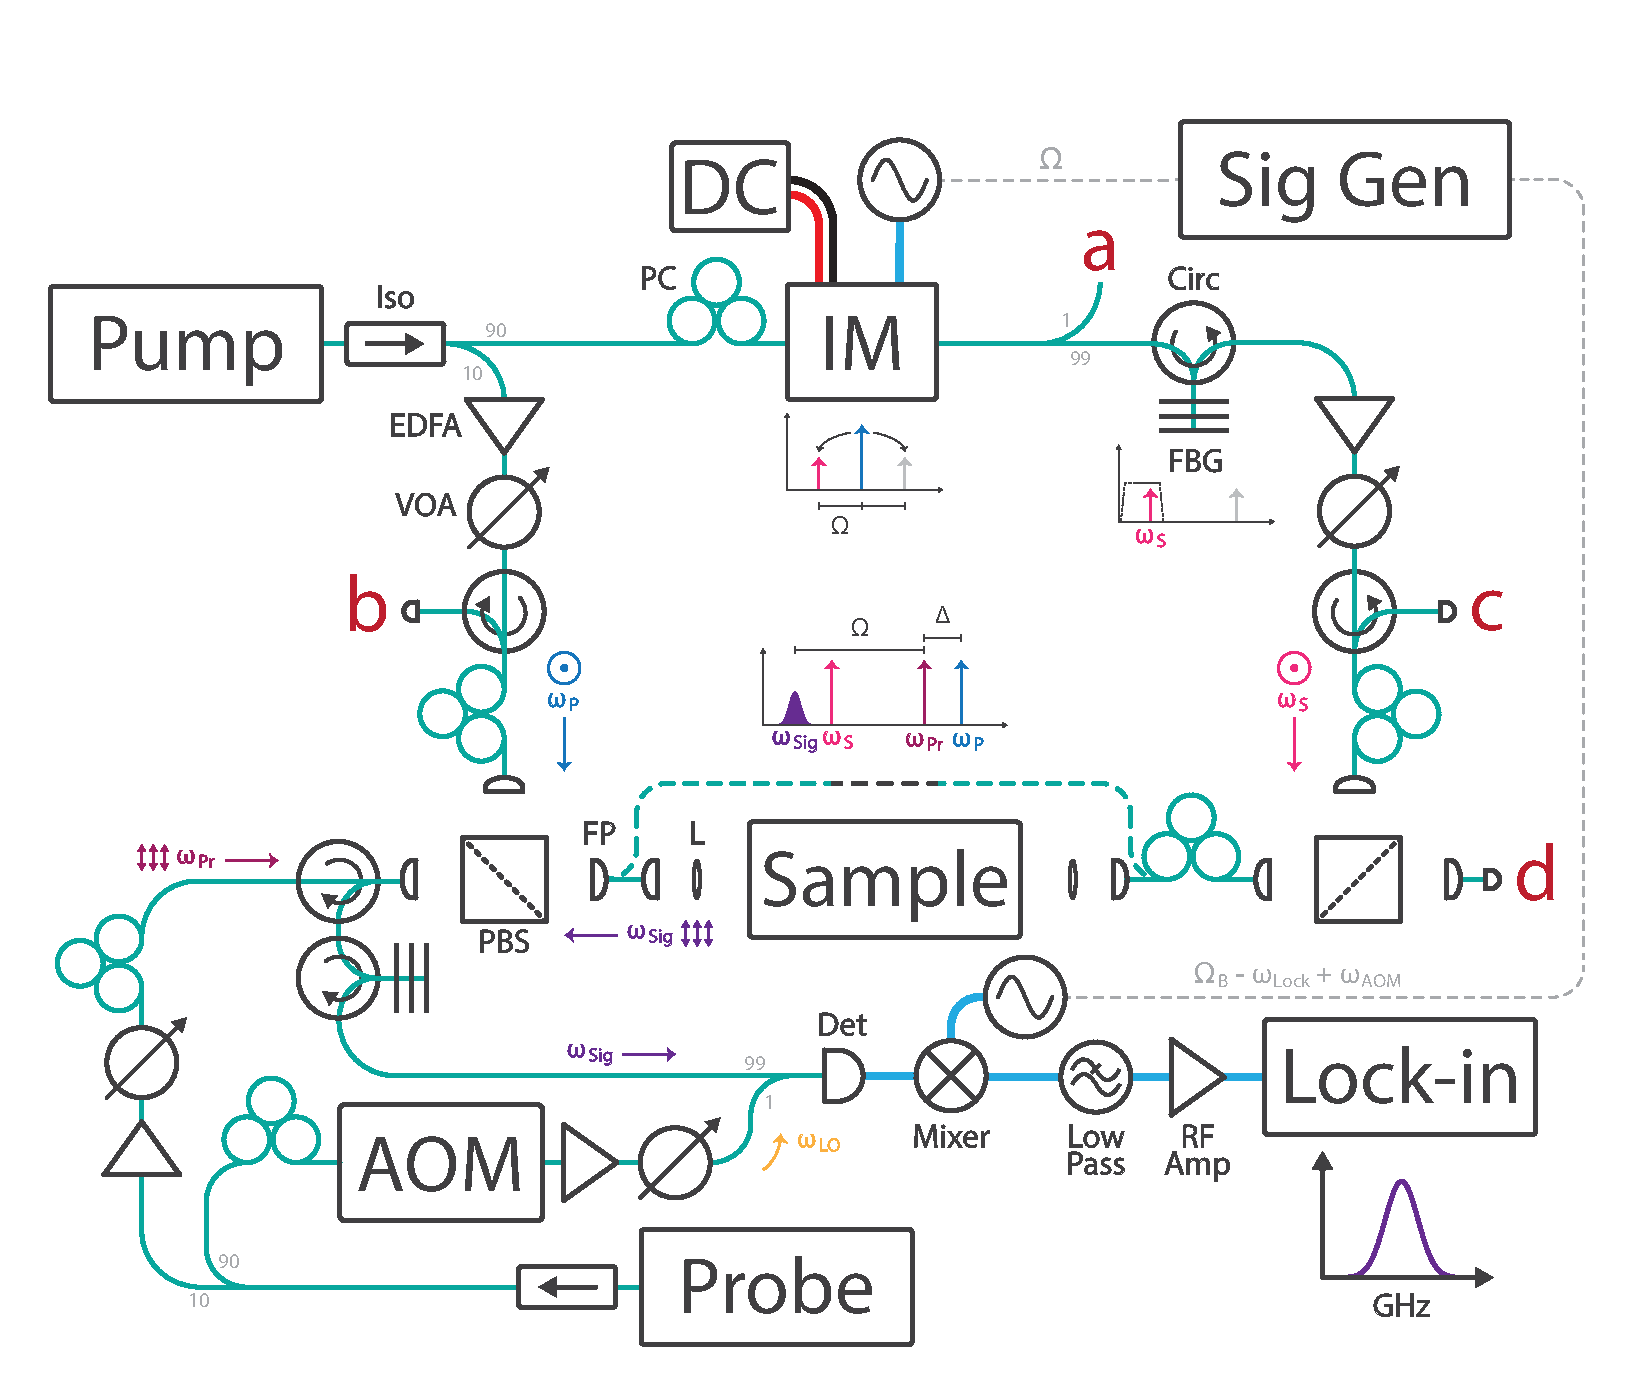
\includegraphics[width=\textwidth]{figs/4-CoBS/Instrument-Design-V1_compat.pdf}
\caption{
Design schematic of a coherently stimulated phonon spectrometer. A tunable \ac{CW} laser at approximately \SI{1.55}{\micro\meter} emits light that passes through an isolator (Iso) and a splitter, diverting 10\% to a \SI{27}{\dBm} \ac{EDFA} followed by a \ac{VOA}. This pump light (\(\omega_P\)) is polarization-controlled to reflect off a \ac{PBS} and is recoupled to fiber via a \ac{FP}, then directed to the sample either by direct fiber coupling or through a pair of \ac{FP}s and lenses (L) for free-space samples. After passing through the sample, the pump light traverses a corrective polarization controller that mitigates fiber twists and bends before reflecting off a second \ac{PBS}, where it is routed to port (c) for power monitoring. To synthesize the Stokes wave, a 90\% split from the original pump is processed through a \ac{IM} and a \ac{FBG}, generating a Stokes sideband downshifted from the pump by \(\Omega\). This frequency shift is swept via a signal generator to capture \(\Omega_B\). A 99/1 splitter provides a tap at port (a) to optimize Stokes synthesis. The Stokes wave (\(\omega_S\)), amplified by a \SI{1}{\watt} \ac{EDFA} and \ac{VOA}-controlled, counter-propagates along the pump path and is monitored at port (b). A second tunable \ac{CW} laser, detuned from the pump, generates the probe wave (\(\omega_{Pr}\)), which is amplified by a \SI{1}{\watt} \ac{EDFA}, attenuated variably, and polarization-controlled to pass through the initial \ac{PBS} where it is incident on the sample. Backscattered signal light (\(\omega_{Sig}\)) transmits back through the \ac{PBS}, while unscattered probe light transmits to a power meter at port (d). A circulator parts the signal from the probe path, with an \ac{FBG} filtering out any unwanted noise or Stokes light. Finally, the signal is heterodyned with an \ac{EDFA}-amplified, \ac{AOM}-shifted \ac{LO} derived from the probe laser and directed to a photodiode for detection. The resulting \ac{RF} signal is mixed with an \ac{AC} \ac{LO} supplied by the signal generator which sweeps synchronously with the Stokes synthesis frequency, and collected by a lock-in amplifier for data processing.
}
\label{fig:Instrument Design}
\end{figure*}

Figure~\ref{fig:Instrument Design} shows the instrument’s design. A pump and Stokes wave is synthesized from a single tunable laser source for coherent stimulation of a sample. The pump wave (\(\omega_{\mathrm{Pump}}\)) is amplified by an \ac{EDFA} and passed through a \ac{VOA} for power control. The output is then polarization-controlled to reflect at a \ac{PBS} for injection into the sample. For Stokes synthesis, an \ac{AC} signal (\(\Omega\)) is supplied to an \ac{IM} with carrier frequency nulled and a tunable filter is used to select the lower-frequency Stokes side band (\(\omega_{\mathrm{Pump}} - \Omega\)). This Stokes light is then amplified by an \ac{EDFA}, passed through a \ac{VOA}, and polarization-controlled to reflect at a second \ac{PBS} for couter-propagation to the pump through the sample.

A separate tunable laser is used to supply a probe wave (\(\omega_{\mathrm{Probe}} = \omega_{\mathrm{Pump}} + \Delta k\)) and \ac{LO}. Probe light is amplified by an \ac{EDFA} and passed through a \ac{VOA} and a polarization controller aligns the polarization for transmission through the first \ac{PBS} whereby it copropagates with the pump through the sample. Backscattered light exits the sample and transmits back through the first \ac{PBS}, whereas the orthogonally polarized Stokes light reflects at this same point to be diverted to a tap for power monitoring. The backscattered signal (\(\omega_{\mathrm{Signal}} = \omega_{\mathrm{Probe}} - \Omega\)) then routes through two subsequent circulators for spectral filtering by a \SI{5}{\giga\hertz} bandpass tunable filter. This filter allows the desired backscattered signal to pass while rejecting any reflected probe light as well as any reflected, transmitted, or backscattered light from the pump or Stokes waves that was not already diverted by the PBS.

The filtered signal then heterodynes via a 99-1 splitter with the LO which is frequency-upshifted by an \ac{AOM} (\(\omega_{\mathrm{LO}} = \omega_{\mathrm{Probe}} + \omega_{\mathrm{AOM}}\)) and controlled to be copolarized with the signal. Of the resulting frequencies from the heterodyne process, only the difference frequency term is considered, as all others are beyond the range of detection. This heterodyned signal (\(\omega_{\mathrm{Signal}} = \Omega + \omega_{\mathrm{AOM}}\)) is then captured by a photodiode detector and heterodyned again by a \ac{RF} mixer with a second \ac{AC} signal (\(\Omega + \omega_{\mathrm{AOM}} - \omega_{\mathrm{Lock}}\)), where \(\omega_{\mathrm{Lock}}\) is a fixed-frequency to be detected by a lock-in amplifier set to this frequency after being passed through a low-pass filter and amplified by an \ac{RF} amplifier. Synchronous sweeping of both \ac{AC} signals, each involving \(\Omega\), allows for \(\omega_{\mathrm{Lock}}\) to remain fixed throughout measurement over a frequency range.

\subsection{Experimental Techniques}
\label{Methods:Experimental Techniques}
We optimized the \ac{SNR} of my instrument through specific design choices and device settings. my setup simultaneously generates pump, Stokes, and probe optical fields for coherently stimulated Brillouin scattering. The pump laser provides \(\sim\!\SI{45}{\milli\watt}\) total output, of which 10\% is split and amplified to \(\sim\!\SI{0.5}{\watt}\) for the pump field; the remaining 90\% is frequency-shifted and amplified to \(\sim\!\SI{1}{\watt}\) for the Stokes field. Likewise, the probe laser also outputs \(\sim\!\SI{45}{\milli\watt}\), with 10\% amplified to \(\sim\!\SI{1}{\watt}\) for the probe field and the remaining 90\% reserved for the \ac{LO}. To combine the backscattered signal and \ac{LO} with minimal loss, weuse a 99/1 splitter instead of a typical 50/50, preserving 99\% of the signal. The \ac{LO} is therefore amplified to \(\sim\!\SI{230}{\milli\watt}\) so the total optical power at the detector remains below the \(\SI{2.4}{\milli\watt}\) damage threshold. After detection, the electronic signal is mixed with a \SI{17}{\dBm} \ac{AC} reference and further amplified by \SI{23}{\dBm} before input to the lock-in amplifier. We find that running both the pump and probe lasers in “whisper” mode (as opposed to “dither”) significantly enhances the measured SNR.

We use a Zurich Instruments HF2LI \SI{50}{\mega\hertz} lock-in amplifier whose demodulator settings are carefully tuned to maximize \ac{SNR}. A \SI{10}{\mega\hertz} reference clock from the signal generator is fed into the lock-in to synchronize timing. The input-signal range, which sets the analog input amplifier’s gain, should exceed the measured signal (including any \ac{DC} offset) by at least a factor of two. This is best achieved by using the lock-in software’s auto feature, which continuously adjusts the range over a rolling \SI{100}{\milli\second} window. We set the input coupling to \ac{AC}, insert a high-pass filter to remove \ac{DC} components, and choose \SI{1}{\mega\ohm} input impedance. For noise suppression, we also engage the lock-in’s eighth-order low-pass filter (roll-off \SI{48}{\decibel\per\octave}) and sample the data at \SI{1.84}{\mega\sample\per\second}, the maximum rate available.

Further \ac{SNR} improvements are gained by narrowing the lock-in’s low-pass filter bandwidth to match both the sub-\si{\hertz} natural linewidth of the heterodyne signal and the thermally-driven frequency drift of the apparatus. After a \(\sim\!\SI{30}{\minute}\) warm-up, we observe less than \SI{100}{\hertz} of drift in the detected signal frequency, so we typically set a \SI{100}{\hertz} low-pass bandwidth for multi-hour measurements. For shorter scans (\(< \SI{15}{\minute}\)), we can reduce this bandwidth to \SI{40}{\hertz} if needed. In addition to linewidth variability, the signal’s center frequency can shift due to thermal changes in the \ac{AOM} and related electronics. Although \(\Omega\) is nominally controlled to sub-hertz precision by the signal generator, our \ac{AOM}’s shift \(\omega_{\mathrm{AOM}}\) drifts from \SI{40}{\mega\hertz} up to \(\sim\!\SI{40.00082}{\mega\hertz}\) over roughly \SI{30}{\minute}. Once at thermal equilibrium, the \ac{AOM} remains stable within \(\pm\SI{50}{\hertz}\), enabling a reliable lock-in frequency reference and minimal filter bandwidth. This stability is crucial for repeatable, high-resolution Brillouin measurements.

\section{Results}\label{Results}
\subsection{Instrument Sensitivity}
\label{Results:Instrument sensitivity and SBS comparison}

We begin by testing the sensitivity of the instrument as a way of defining a performance metric for the instrument which can be used to indicate what material, power, and length combinations might be possible to measure. From Equation~\ref{Eq:Theoretical Framework:Scattered Power}, the sensitivity of the instrument is the minimum scattered power, \(P_{Sig}\), to produce a statistically significant measurement. To determine this, we target a specific length, \(L\), of a sample of known effective Brillouin gain, \(G_B\). We keep the pump-probe detuning, \(\Delta\lambda\), constant across measurements and record the pump, Stokes, and probe optical powers to calculate the scattered power. Starting with sufficient optical powers to produce a clearly distinguishable measurement, we gradually reduce the optical powers until the sensitivity floor is reached.

To serve as our sensitivity testbed, we prepared \SI{1}{\centi\meter} of Nufern's \ac{UHNA3} fiber, a well-studied fiber with known effective Brillouin gain\cite{behunin2015long}. Additionally, \ac{UHNA3} fiber offers several properties that make it ideal for this task of unambiguous detection of the Brillouin signal as it diminishes with each subsequent reduction in optical powers. First, it offers a Brillouin shift that is spectrally far from that of the \ac{SMF-28} which constitutes much of the instrument. This ensures that the Brillouin response of the sample is not conflated with the Brillouin response of the instrument itself. Additionally, the core of \ac{UHNA3} fiber features a high concentration of germanium which improves the optical and acoustic guidance in the fiber as a result of the large refractive index difference between core and cladding. Finally, \ac{UHNA3} fiber offers a high optomechanical nonlinear response, with an effective Brillouin gain of \SI{0.6}{\per\watt\per\meter} measured at room temperature\cite{behunin2015long}. This gain factor is larger than that of \ac{SMF-28} by an order of magnitude\cite{nikles1997brillouin}.

\begin{figure}[t!]
  \centering
  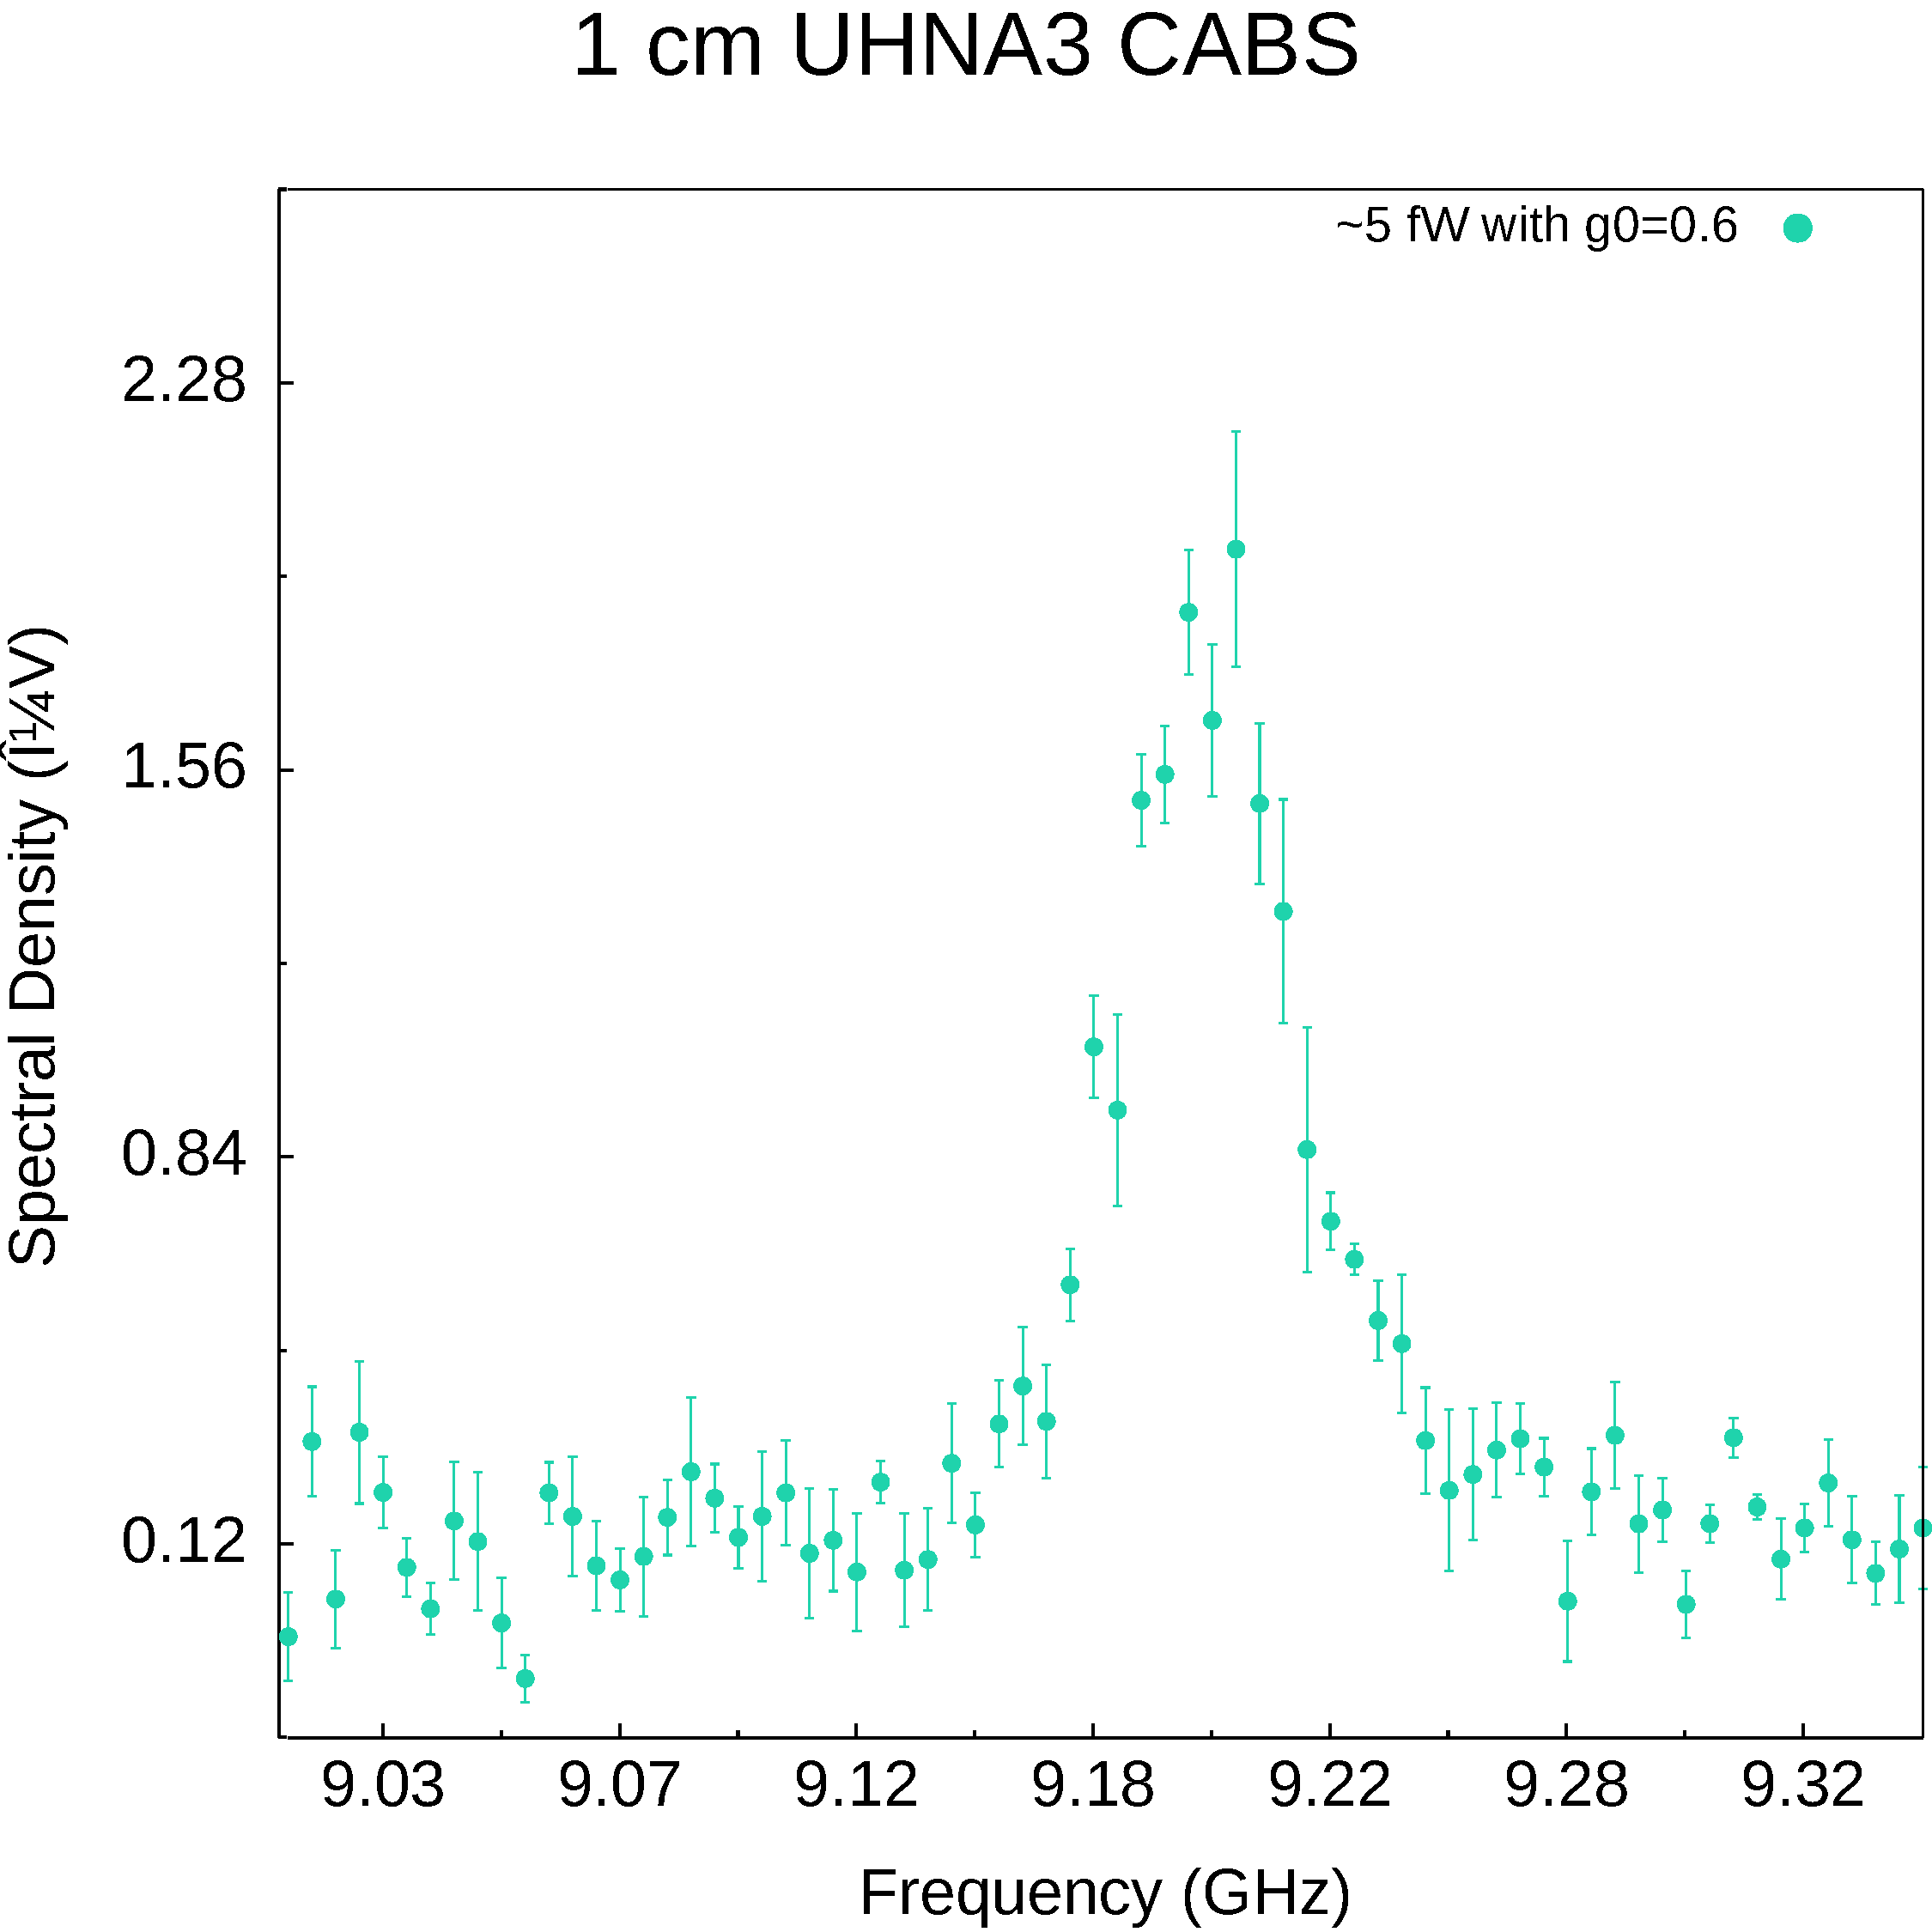
\includegraphics[width=\textwidth]{figs/4-CoBS/5fWSensitivity.pdf}
  \caption{\(\sim\SI{5}{\femto\watt}\) sensitivity measurement}
  \label{fig:5fWSensitivity}
\end{figure}

Figure~\ref{fig:5fWSensitivity} presents a measurement in which the instrument’s sensitivity reaches \(P_{Sig}\!= \SI{5}{\femto\watt}\). Each trace is the average of five consecutive scans, and an average of five background scans has been subtracted to isolate the signal. Error bars represent the standard error (\(1\sigma\) of the mean). By comparing the peak amplitude at resonance to the off-resonance baseline, we estimate an \ac{SNR} greater than 5. Under a normal-noise assumption, an \ac{SNR} of 5 corresponds to a \(5\sigma\) significance level (99.7\% confidence). Achieving this \SI{5}{\femto\watt} threshold demonstrates the feasibility of measuring weaker signals in materials with lower Brillouin gain or smaller effective lengths.

\begin{table}[h]
    \centering
    \caption{Measurement parameters for sensitivity measurement and calculation.}
    \begin{tabular}{c c c c c c}
        \toprule
        \(\mathbf{G_{\mathrm{\textbf{B}}}}\) &
        \(\textbf{L}\) &
        \(\mathbf{P_{\mathrm{\textbf{P}}}}\) &
        \(\mathbf{P_{\mathrm{\textbf{S}}}}\) &
        \(\mathbf{P_{\mathrm{\textbf{Pr}}}}\) &
        \(\mathbf{\Delta\lambda}\) \\
        (\si{\per\watt\per\meter}) &
        (\si{\meter}) &
        (\si{\micro\watt}) &
        (\si{\micro\watt}) &
        (\si{\micro\watt}) &
        (\si{\pico\meter}) \\
        \midrule
        0.6 & 0.01 & 506 & 504 & 2.01 & 20 \\
        \bottomrule
    \end{tabular}
    \label{tab:sensitivity}
\end{table}

\subsection{Measurements}
\label{Results:Measurements}

We demonstrate the capabilities of the instrument on two common sample classes: fiber and bulk material. For a fiber sample we again choose UHNA3 for its higher nonlinear response and excellent optical and acoustic guidance. In contrast to the sensitivity measurements, we now seek to demonstrate the full measuring capabilities of the instrument and so apply all available optical power (\(\sim\!\SI{1.5}{\watt}\)) to maximize the backscattered signal from the sample. We target the same \SI{1}{\centi\meter} segment of \ac{UHNA3} fiber as was used for determining sensitivity.

\begin{figure}[t!]
  \centering
  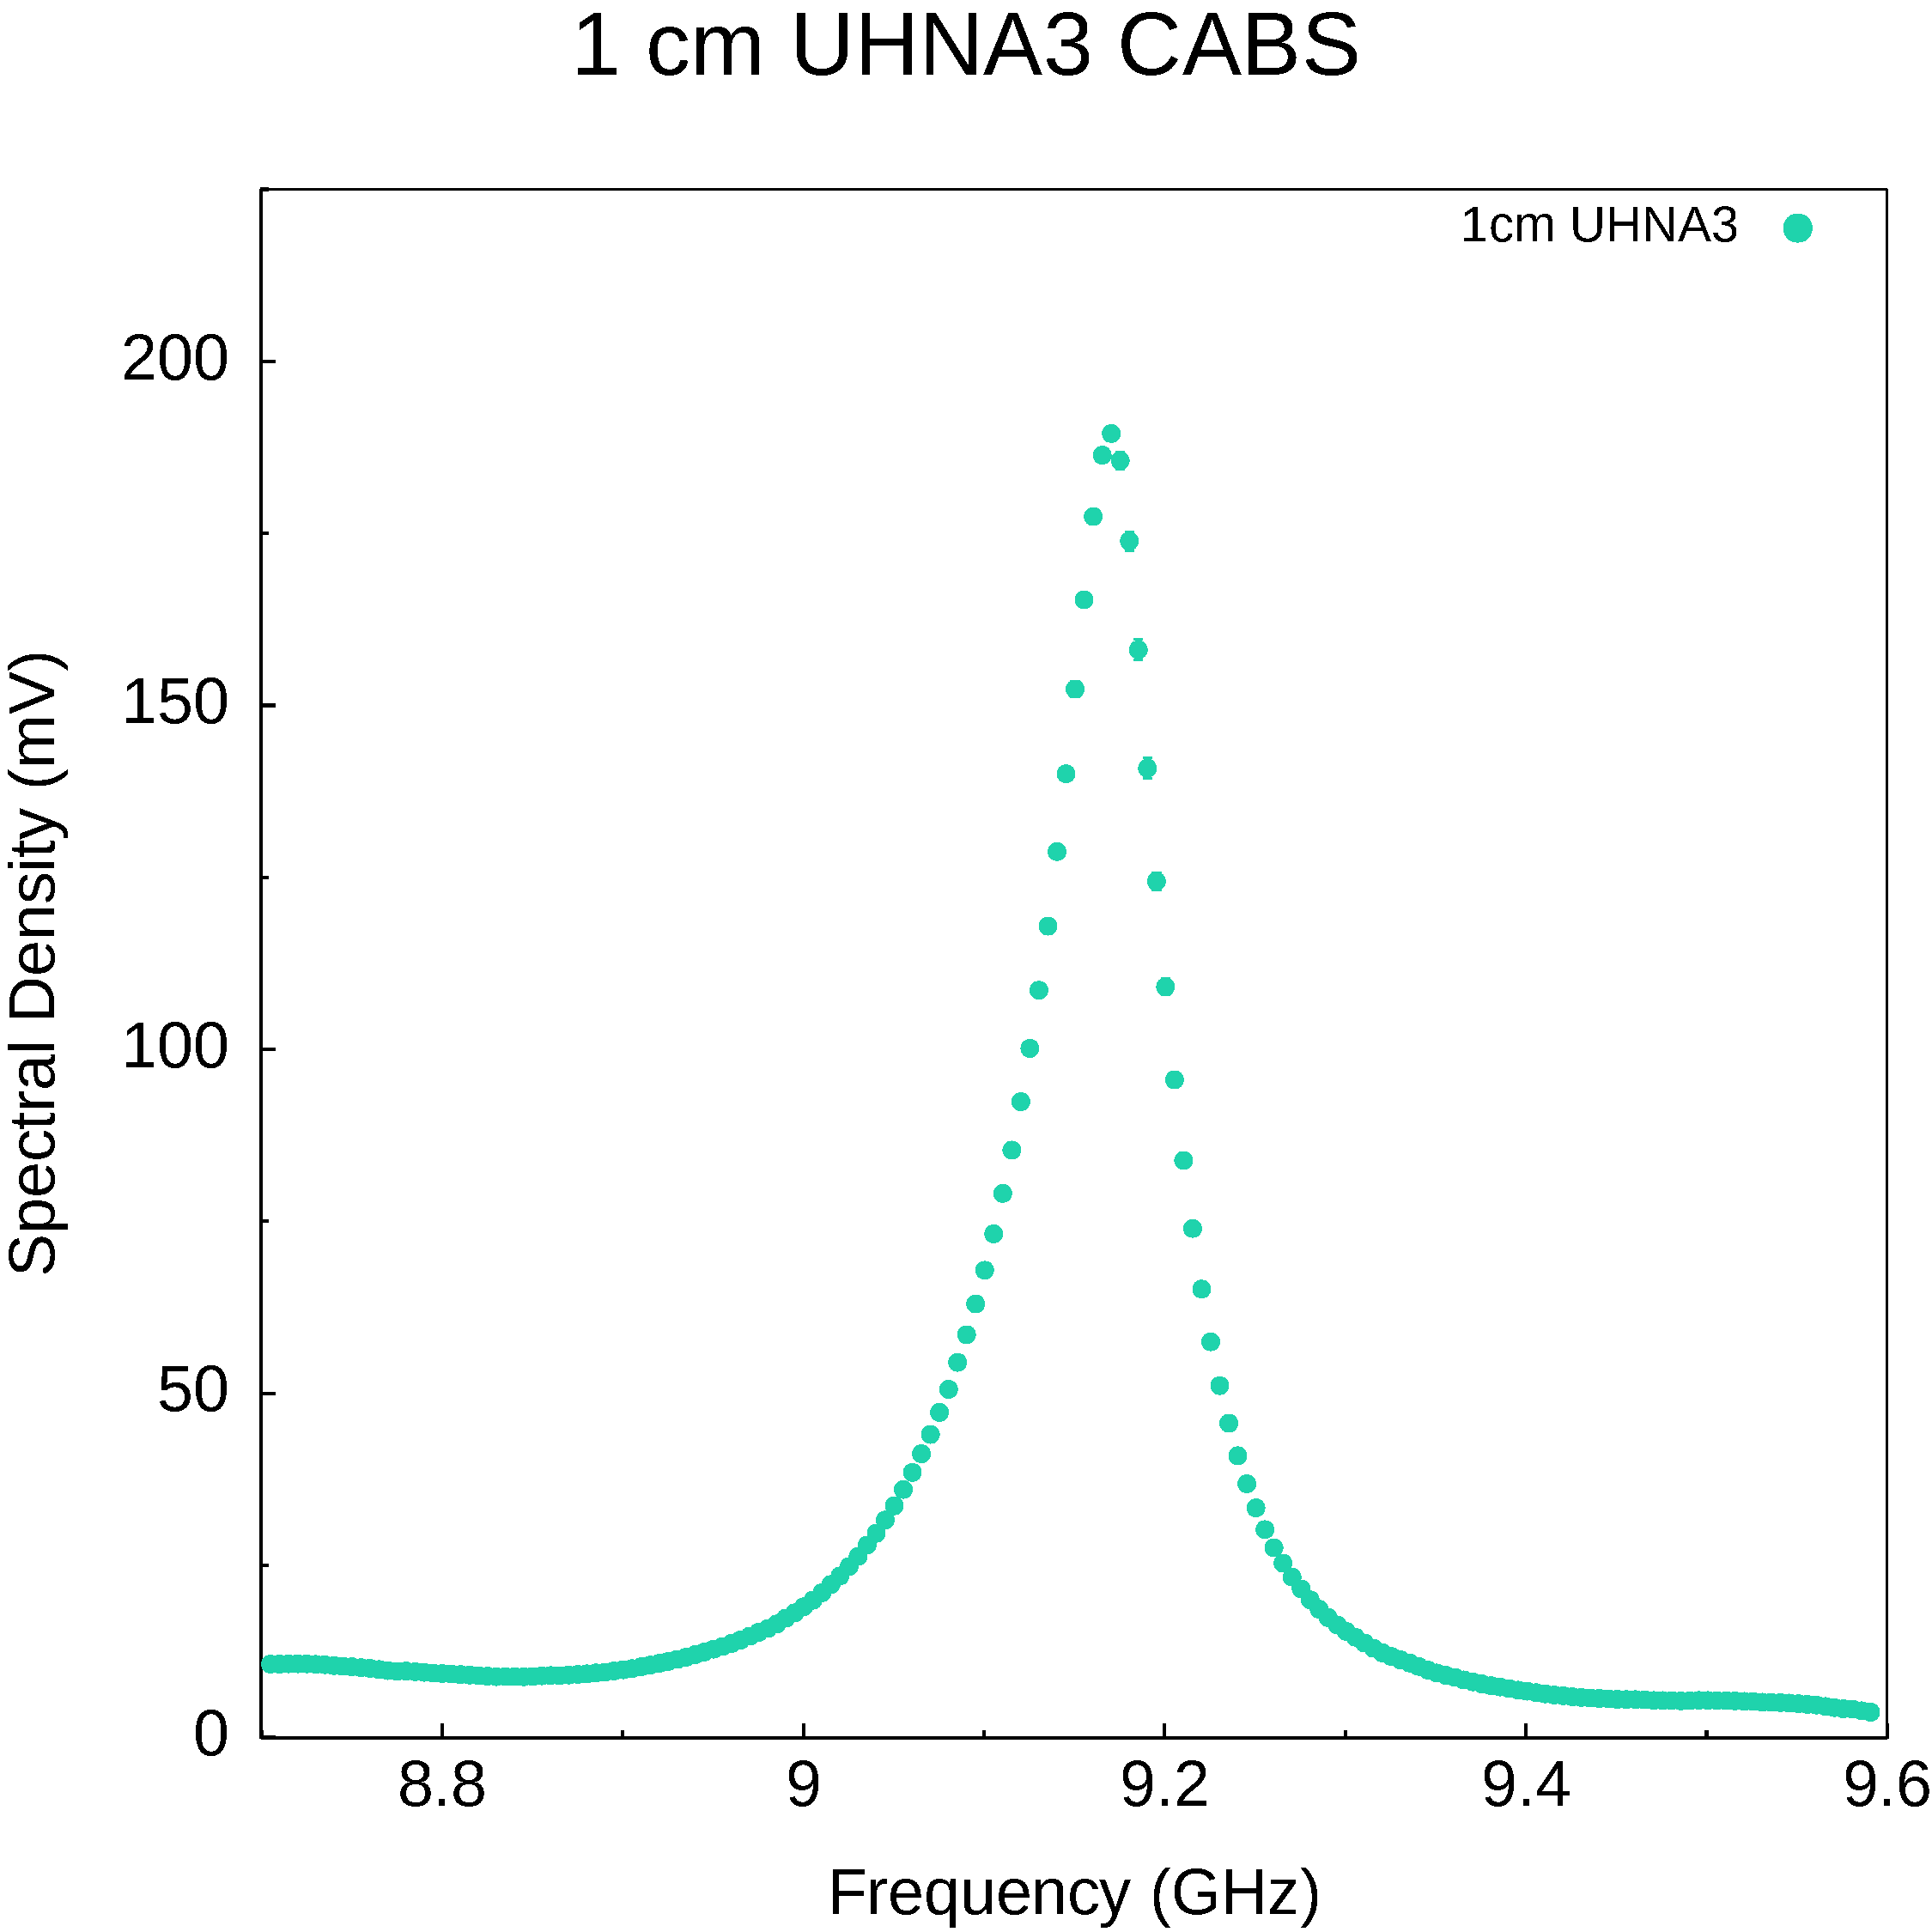
\includegraphics[width=\textwidth]{figs/4-CoBS/1cmUHNA3.pdf}
  \caption{\SI{1}{\centi\meter} UHNA3}
  \label{fig:1cmUHNA3}
\end{figure}

Figure~\ref{fig:1cmUHNA3} shows the spectral profile captured for \SI{1}{\centi\meter} of \ac{UHNA3} fiber, revealing the expected lorentzian profile consistent with Equation~\ref{Eq:Effective Brillouin Gain}. The peak amplitude of the spectra occurs at \SI{9.1704}{\giga\hertz}, indicating the Brillouin resonance frequency of the longitudinal traveling-wave mode in the fiber. The FWHM of the measurement is \SI{80}{\mega\hertz} and provides a measure of the phonon dissipation rate. Both values match what is seen in the literature for \ac{SBS} measurements of \ac{UHNA3} fiber.\cite{behunin2015long} The data shown are a background-subtracted average of five successive measurements taken over ten minutes with error bars corresponding to \(1\sigma\) of the mean.

To achieve this measurement of \ac{UHNA3} fiber, the instrument design was altered to include only fiber-coupled segments connecting the fiber ports between the two \ac{PBS}s. We set the pump laser wavelength to \SI{1549.000}{\nano\meter} and the probe laser wavelength to \SI{1549.020}{\nano\meter}, giving a frequency mismatch of approximately \SI{2.5}{\giga\hertz}. The pump--probe mismatch is chosen to be only as large as needed to allow the edge of the pass-band of the probe filter to split the backscattered pump and probe light, thus rejecting any backscattered light from the pump laser and accepting only the backscattered signal from the probe laser. We placed the Stokes filter at \SI{1549.073}{\nano\meter}, an offet of approximately \SI{9.18}{\giga\hertz} from the pump laser to capture the Stokes sideband from the intensity modulator. This corresponds to the center of the measured frequency range and was chosen to allow the Stokes sideband output from the intensity modulator to remain within the pass band of the Stokes filter as the RF signal fed to the intensity modulator is swept through the full measurement range. The probe filter was set to \SI{1549.109}{\nano\meter}, an offset of approximately \SI{11.18}{\giga\hertz} from the probe laser, to capture the Stokes-shifted backscattered signal from the probe. The center frequency of the backscattered signal is of course shifted \SI{9.18}{\giga\hertz} from the probe laser, however an extra offset of \SI{2}{\giga\hertz} is chosen for improved rejection of any pump light as the pass band of our filter extends approximately \SI{2.5}{\giga\hertz} on either side of center.

\begin{figure}[t!]
  \centering
  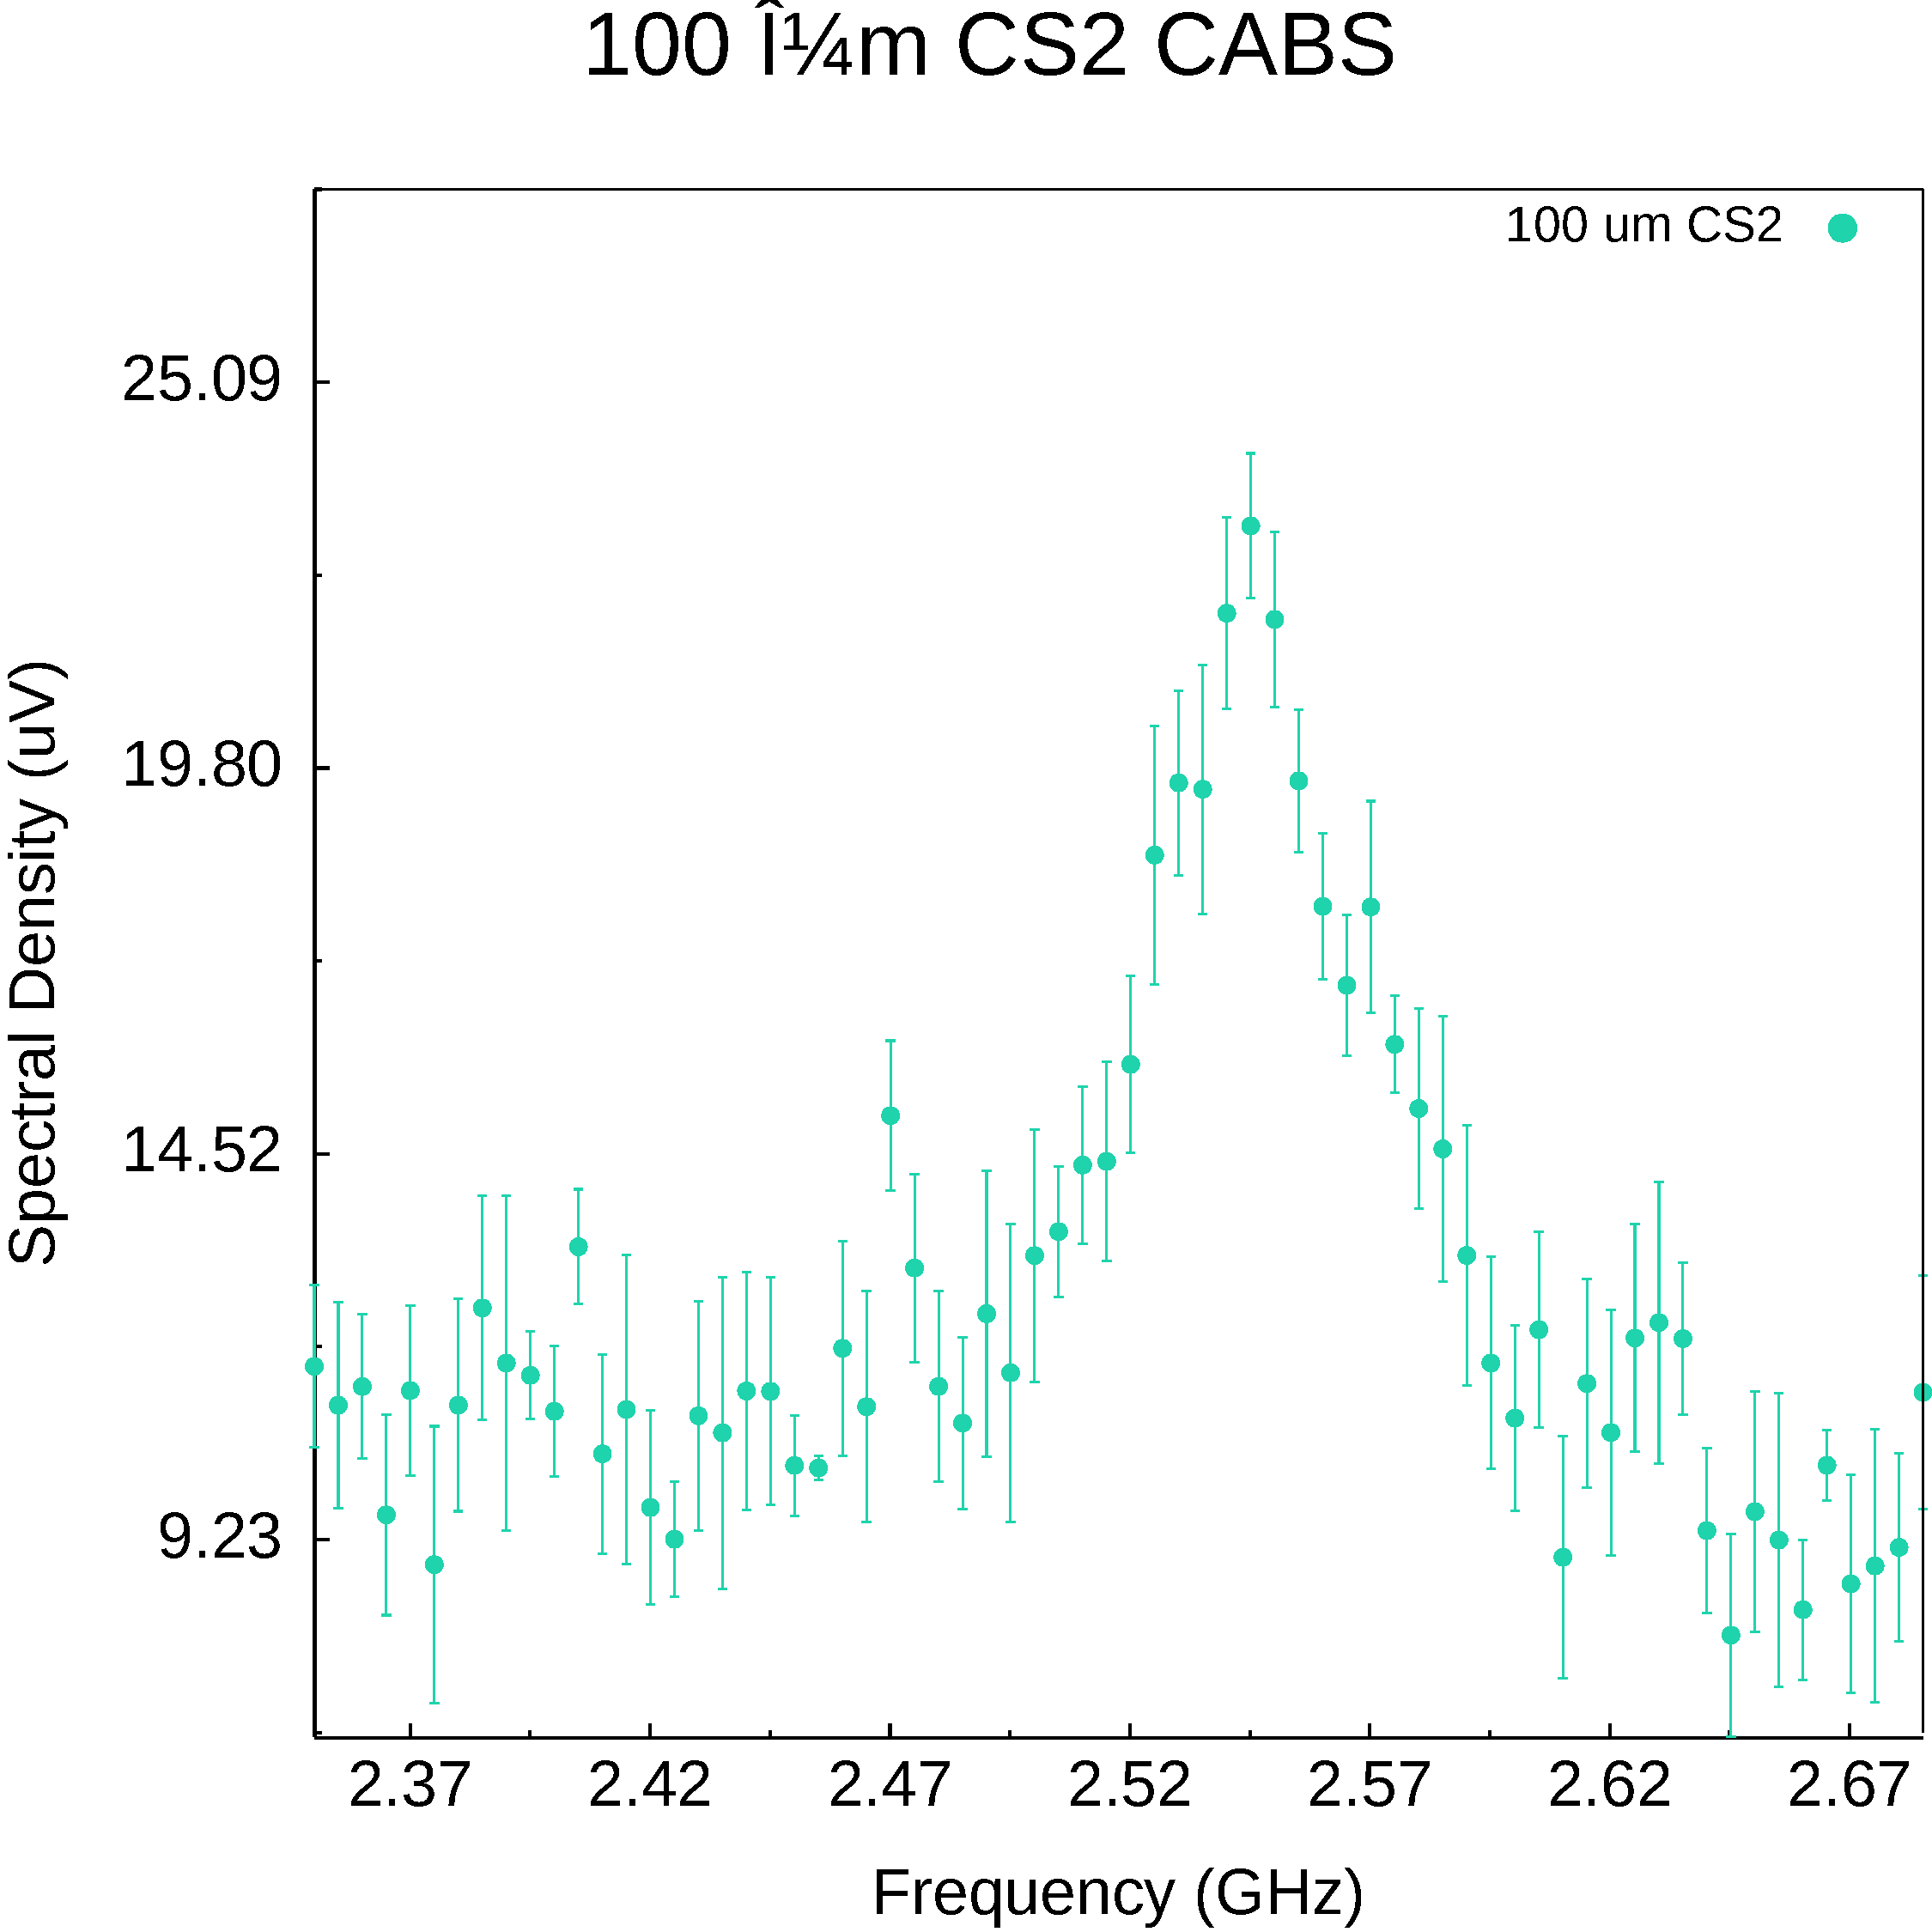
\includegraphics[width=\textwidth]{figs/4-CoBS/100umCS2.pdf}
  \caption{\SI{100}{\micro\meter} \ce{CS2}}
  \label{fig:100umCS2}
\end{figure}

For a free-space bulk example we target liquid \ce{CS2} for its exceptionally high Brillouin gain factor of \SI{1.5}{\meter\per\giga\watt}.\cite{boyd2020nonlinear} Figure~\ref{fig:100umCS2} reveals the Brillouin signal of bulk \ce{CS2} liquid contained in a \SI{100}{\micro\meter} path length cell. To our knowledge, measurement of longitudinal Brillouin scattering at this scale has not been reported in the literature. A scattered power comparison would reveal that achieving such a measurement using traditional \ac{SBS} techniques would require excessively high optical powers or cooling the material to cryogenic temperatures, which, of course, would be prohibitive for carbon disulfide in the liquid state.

For this measurement of \ce{CS2}, the pump and probe laser wavelengths were set to \SI{1548.808}{\nano\meter} and \SI{1548.898}{\nano\meter}, respectively. The short path length of the sample significantly broadens \(\Phi\), the \(\mathrm{sinc^2}\) term defining the phasematching bandwidth, allowing for further separation of the pump and probe wavelengths for improved signal isolation without significant reduction in scattered power of the signal produced in the \ce{CS2}. Specifically, the additional pump--probe wavelength separation of \SI{70}{\pico\meter} employed for this measurement compared to the UHNA3 measurement results in a negligible 0.045\% reduction in scattered power. This additional separation contributes meaningfully, however, to improved rejection of pump light by the probe filter and thus higher SNR of the signal.

Placement of the Stokes filter is critical for measurements of materials that give small Brillouin shifts, such as with \ce{CS2} \SI{2.55}{\giga\hertz} shift. We offset our \SI{5}{\giga\hertz} bandwidth Stokes filter an additional \SI{2}{\giga\hertz} to ensure the nearby carrier signal and anti-Stokes sideband from the intensity modulator are rejected and only the Stokes sideband is allowed to pass. For the measurement shown in Figure~\ref{fig:100umCS2}, this corresponds to a Stokes and probe filter placement of \SI{1548.844}{\nano\meter} and \SI{1548.934}{\nano\meter}, respectively.

% Figure~shows the spectral measurements achieved by the instrument, overlaid with finite-difference simulation data. In Figure~we see the expected lorentzian spectral shape in good alignment with simulation data for guided longitudinal modes in the core of the UHNA3 fiber. In Figure~, however, we see a distortion of this lorentzian shape. This is expected for partially unguided longitudinal modes, such as is the case for a bulk liquid filling the volume of a ...
%
% Figure~\ref{fig:1cmUHNA3} shows a measurement of 1cm of UHNA3 fiber.
%
% First, we measured Brillouin scattering in a 1-centimeter-long UHNA3 fiber at room temperature and with sub-Watt optical power (Figure~). Figure~, clearly displays the Brillouin scattering features with remarkable SNR, highlighting the effectiveness of our apparatus in isolating the backscattered probe light. This observation serves as one of the main showcases of the instrument's capability.
%
% Next, we performed Brillouin scattering measurements on a 4-millimeter-thick bulk carbon disulfide sample in a free-space optics arrangement. The observed spectrum, presented in Figure~2, exhibits well-resolved Brillouin scattering peaks. This successful measurement in a bulk sample demonstrates the versatility and adaptability of our instrument to various experimental configurations, further emphasizing the instrument's capability.
%
% Lastly, we conducted a measurement in a 1-millimeter-long UHNA3 fiber under low-power conditions, with only 10 microwatts of power at the sample. Despite the reduced sample length and low power, the instrument's sensitivity allowed us to observe distinct Brillouin scattering features in the spectrum, as illustrated in Figure~3. This result underscores the potential of our spectrometer for nanoscale measurements and serves as a demonstration of the instrument's sensitivity, defining the sensitivity floor of the apparatus.
%
% These three observations collectively showcase the high sensitivity, broad applicability, and impressive capabilities of our coherent stimulated phonon spectrometer in measuring Brillouin scattering across different sample types, scales, and power levels.

\subsection{Phase Matching Bandwidth}
\label{Results:Phase Matching Characterization}

To characterize the phase matching tolerance of the instrument for a given length of sample, we performed an additional experiment whereby we took a series of measurements of \SI{1}{\centi\meter} of UHNA3 at constant optical powers while letting the detuning of the pump and probe lasers vary. In the language of Equation~\ref{Eq:Theoretical Framework:Scattered Power}, this experiment holds \(G_B\), \(L\), \(P_P\), \(P_S\), and \(P_{Pr}\) constant while letting \(\Delta k\) vary. For the experiment to support the validation of Equation~\ref{Eq:Theoretical Framework:Scattered Power}, we would expect the peak amplitudes of these measurements to trace out a \(\mathrm{sinc^2}\) profile, also given by Equation~\ref{Eq:Phi}. Figure~\ref{fig:Phase-Match} shows the results of this experiment. We performed 75 measurements between \SI{5}{\giga\hertz} and \SI{42}{\giga\hertz} pump--probe detuning, at \SI{0.5}{\giga\hertz} intervals. We found peak amplitudes by fitting each spectra with a Fano profile (see Section~\ref{Results:Fano-Resonant Asymmetries at Small Signals}) and represented each peak as a data point in Figure~\ref{fig:Phase-Match}. The theoretical \(\mathrm{sinc^2}\) function matching the parameters used in the experiment is shown on the plot with a solid red line.

%Describe adjustments and/or explain deviations from pure sinc^2 (noise floor, Fano effects, L uncertainty, etc.), or reference Fano section

\begin{figure}[t!]
\centering
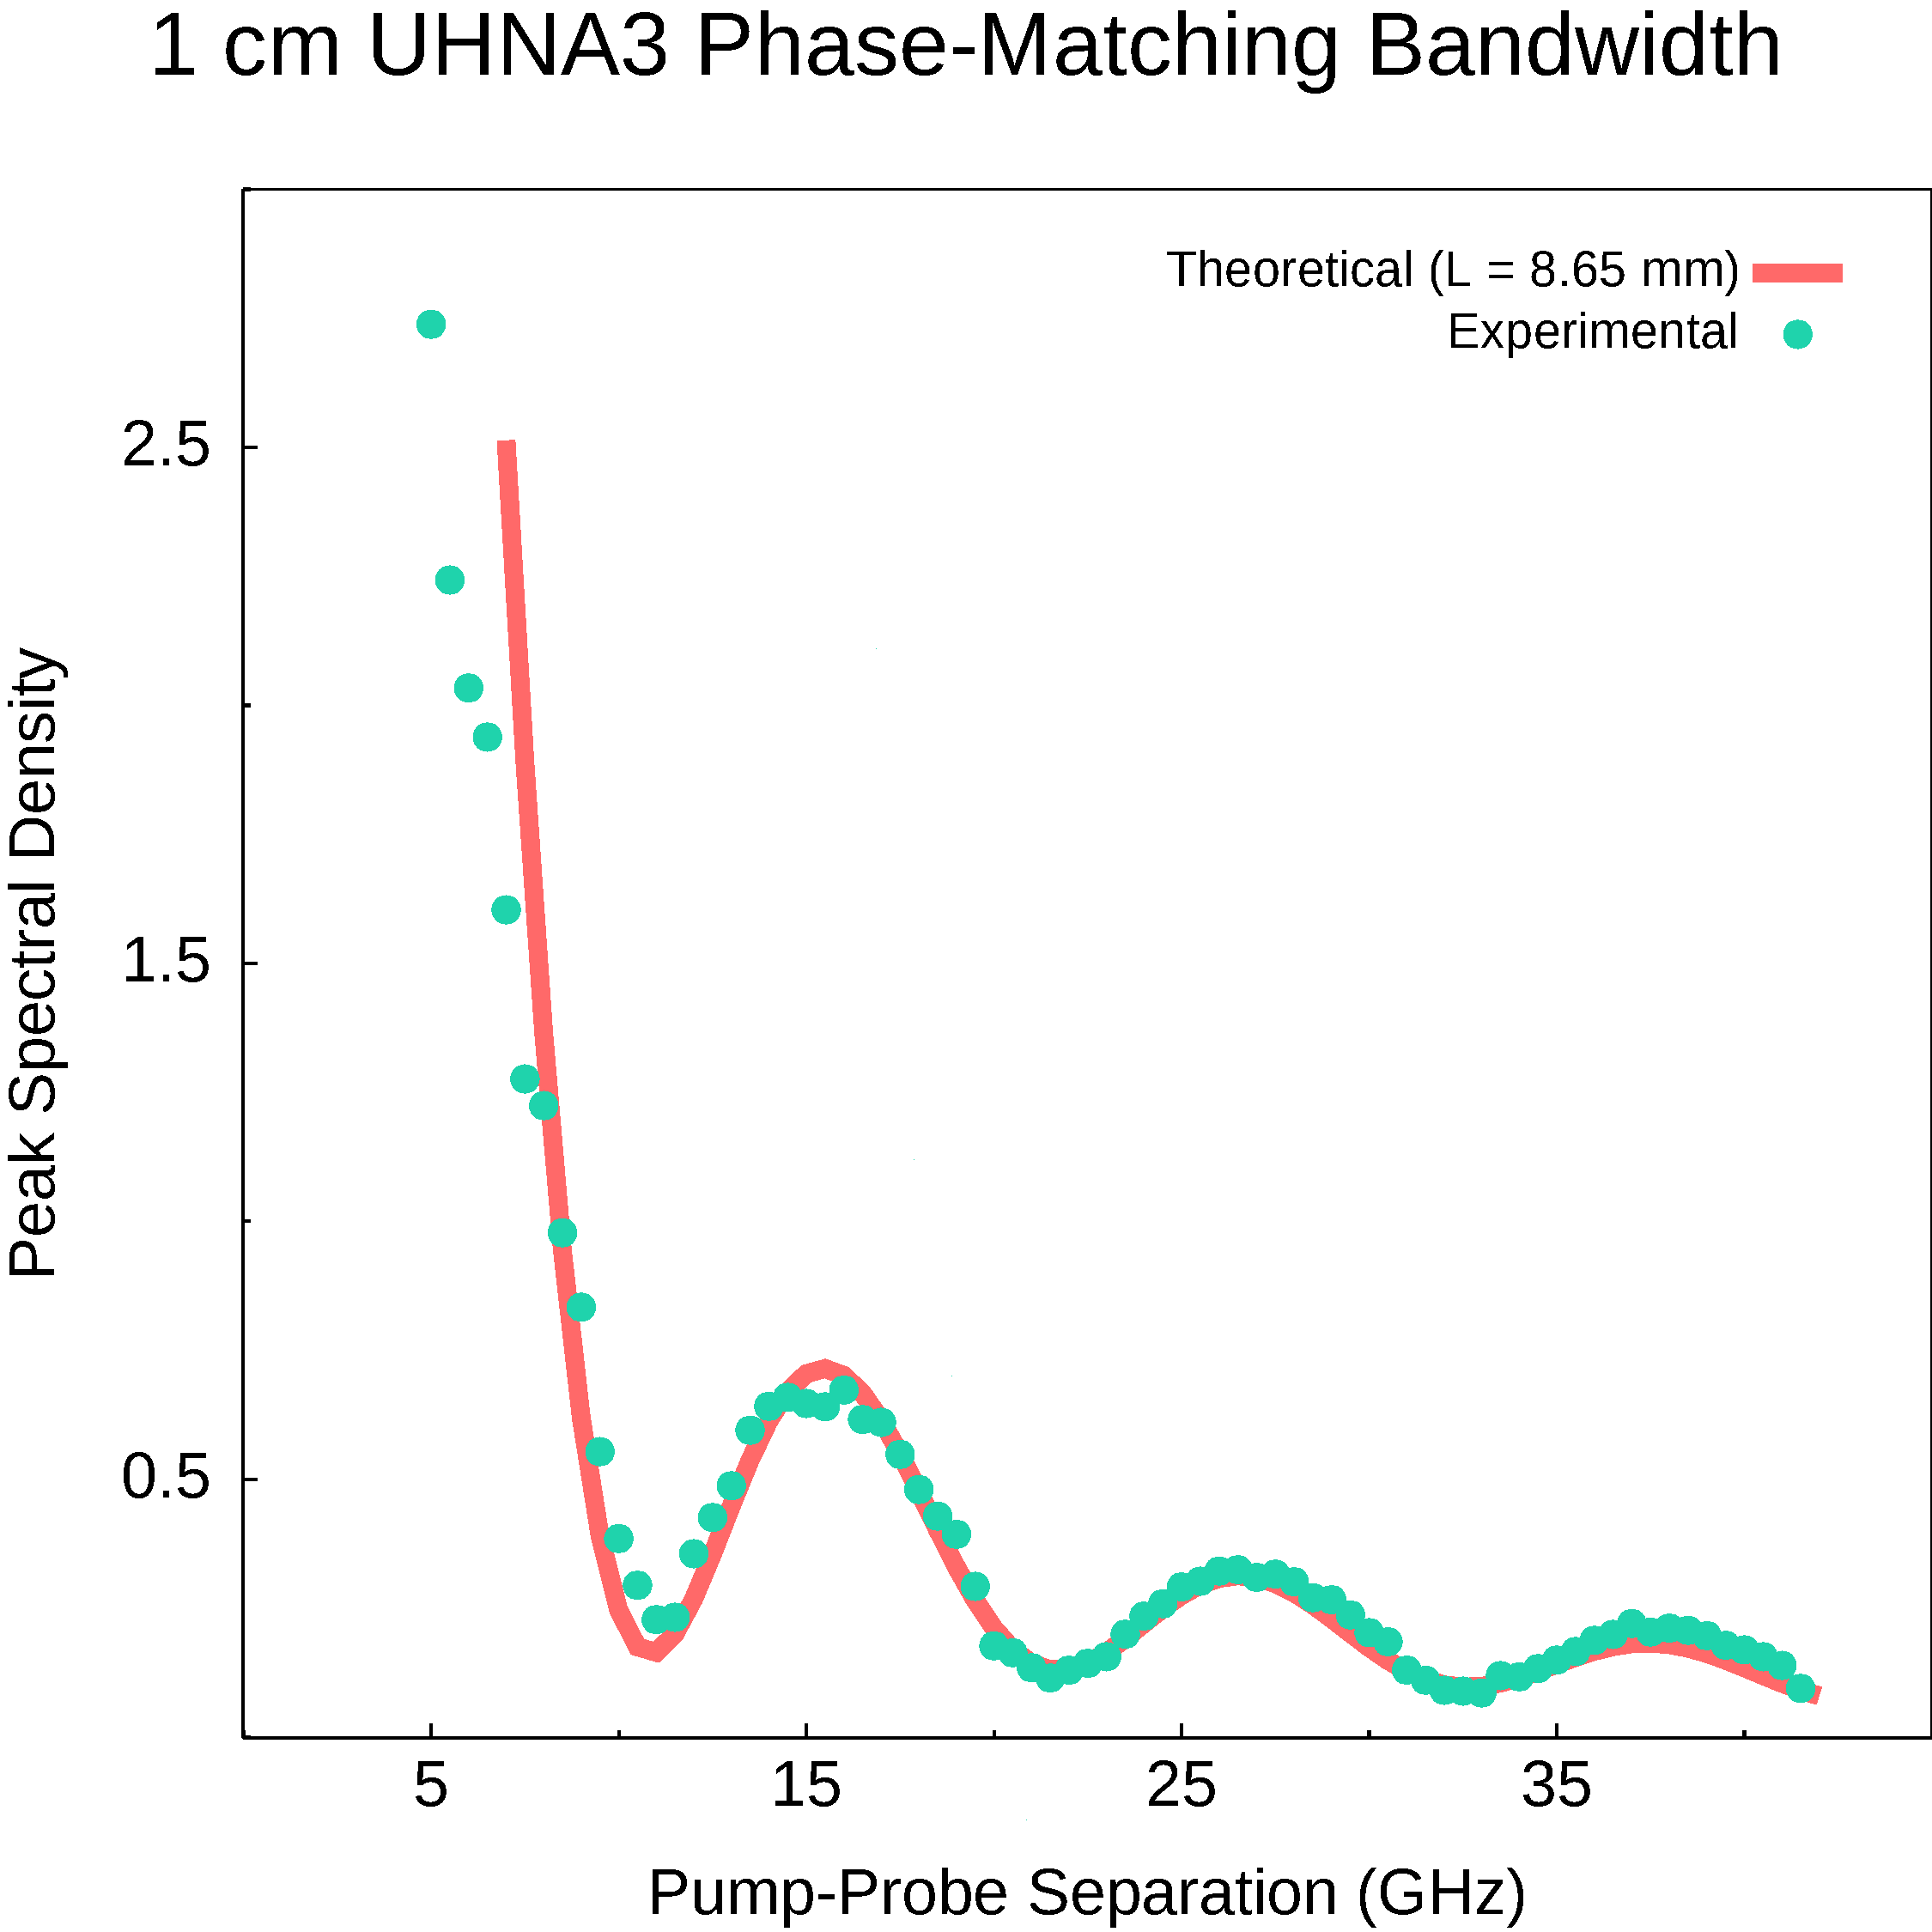
\includegraphics[width=\textwidth]{figs/4-CoBS/Phase-Match.pdf}
\caption{Phase-matching \(\mathrm{sinc^2}\) func}
\label{fig:Phase-Match}
\end{figure}

\subsection{Fano-Resonant Asymmetries at Small Signals}
\label{Results:Fano-Resonant Asymmetries at Small Signals}

Under certain conditions where the resonant Brillouin amplitude approaches the background continuum level, we observe an asymmetric, Fano‐type line-shape \cite{fano1961effects, limonov2017fano, limonov2021fano, kroner2008nonlinear}. These Fano distortions can shift the apparent peak frequency, complicate simple Lorentzian fitting, and affect the extracted linewidth in small‐signal measurements. \cite{miroshnichenko2010fano} To properly handle these occurances, it is necessary to understand when they are likely to arise with this technique and how they may be corrected for or controlled. Fano resonances arise when a discrete resonance (in our case, the Brillouin mode) interferes with a continuum background (e.g., noise floor or broad, non‐resonant scattering). When the resonance amplitude is no longer much larger than the continuum, the interference leads to an asymmetric line-shape described by the Fano formula \cite{fano1961effects},

\begin{equation}
I(\omega) \propto \frac{(q + \epsilon)^2}{1 + \epsilon^2},
\label{eq:fano}
\end{equation}

where \(\epsilon \equiv (\Omega - \Omega_{B})/(\Gamma_{B}/2)\) is the dimensionless detuning from the Brillouin peak (measured in half the spectral linewidth) and \(q\) is the Fano asymmetry parameter. The Fano asymmetry parameter captures the ratio of the resonant scattering to the background scattering amplitudes as well as the relative phase of each. It can be defined as

\begin{equation}
  q = \frac{(\mathrm{resonant amplitude})}{(\mathrm{background amplitude})}\cot{(\Delta\phi)},
\end{equation}

where \(\Delta\phi\) is the phase difference between the oscillation driven by the discrete resonant mode and that of the background continuum \cite{limonov2017fano, ko2023full, gu2020fano}.

In the event of Fano interference, the complex background amplitude often varies slowly with energy and can be seen as having a fixed phase reference, while the resonant amplitude undergoes a rapid \(\pi\) phase change as the energy passes through the resonance. \cite{limonov2017fano} When the resonant and background contributions are exactly out of phase at the resonance frequency (phase difference \(\Delta\phi = \pi/2\), meaning destructive interference), the spectral line exhibits a dib to zero (anti-resonance) at the discrete resonance frequency, corresponding to \(q=0\) in Equation~\ref{eq:fano}. If they are exactly in phase (\(\Delta\phi = 0 or \pi\), fully constructive interference at resonance), the resonance appears purely Lorentzian without asymmetry and \(|q| \to \infty\). For intermediate phase offsets, one lobe of the resonance is enhanced while the other is suppressed, yielding an asymmetric peak or dip with finite \(q\). The sign of q indicates the direction of asymmetry (which wing of the resonance is enhanced). A positive \(q\) means the discrete mode \textit{leads} the background in phase. In this case, the spectral profile has a sharp rise on the low-frequency side and a more gradual fall-off on the high-frequency side. Conversely, a negative \(q\) means the discrete mode \textit{lags} the background in phase, leading to a flipped orientation featuring a sharp rise on the \textit{high}-frequency side and a gradual fall-off on the \textit{low}-frequency side.

We first noticed this behavior appearing in our small-length \ce{CS2} data, where a small shift in probe wavelength revealed an asymmetric line-shape. For the measurements of \SI{100}{\micro\meter} \ce{CS2} (Figure~\ref{fig:100umCS2}) and \SI{1}{\centi\meter} \ac{UHNA3} fiber at low power (Figure~\ref{fig:5fWSensitivity}), the amplitude of the resonant Brillouin peak is on the order of that of the non‐resonant continuum, giving a strong chance for Fano interference. Whenever \(\tfrac{I_{\text{res}}}{I_{\text{bkg}}}\approx 1\), the parameter \(q\) as given by Equation~\ref{eq:fano} can become finite rather than \(\pm \infty\) in the limit that the background is negligible, and Fano interference arises. To explore this further, we performed a similar phase-matching experiment as was done for \SI{1}{\centi\meter} \ac{UHNA3} (see Phase Matching Bandwidth subsection), this time with \SI{1}{\milli\meter} of \ce{CS2}. Results from this experiment are presented in Appendix~\ref{Appendix:Fano} and offer examples of line shapes with pronounced asymmetry and featuring clear characteristic morphologies associated with Fano interference. These pronounced distortions in spectral line shape for small signal measurements underscore the role Fano interference in small resonant amplitudes relative to the background.

Because our instrument offers sub-\SI{10}{\femto\watt} sensitivity signal amplitudes have the potential to approach the order of the background continuum amplitude. For this reason, and because the instrument offers an advantage in measurements of samples of short length (\(<\)\SI{10}{m}) (see Appendix~\ref{appendix:comparison}), Fano effects may often arise with usage of this technique and must be handled appropriately. This includes properly fitting data with a Fano profile as opposed to a Lorentzian to ensure accurate capture of relevant parameters such as linewidth, resonant frequency, and peak amplitude. Beyond fitting and parameter extraction, it is important to be mindful that these effects are likely to occur in ambitious measurements at the limits of equipment sensitivity. Expectation and proper handling of Fano effects in measurements of this nature ensures that they may be more easily recognized and confirmed, as the data is likely to present a spectrum that deviates considerably from the standard Lorentzian. Appendix~\ref{appendix:comparison} offers a comparative analysis of two example spectra featuring highly assymetric profiles fitted with a naïve Lorentzian vs. a more appropriate Fano function.

In some cases, and of particular interest for ambitious measurements, Fano interference may even \textit{boost} the measured peak above the naïve Lorentzian amplitude—i.e., ‘amplify’ it—when \(q \neq 0\). In principle, a Fano‐type lineshape can exhibit a locally higher peak amplitude than a pure Lorentzian if the discrete Brillouin response constructively interferes with the background continuum near the resonance. Crucially, this does not represent net energy gain but rather a redistribution of intensity through interference. Although the resonance peak may appear taller, the continuum also contributes noise and can partially interfere destructively elsewhere, so the global \ac{SNR} may or may not improve. Nonetheless, our technique offers the ability to dynamically tune the phase of the Brillouin response relative to the background via adjustment of the probe laser wavelength. This interference-tuning of the continuum and discrete components allows some control over constructive or destructive interference. Moreover, we can achieve this without sacrificing independent control of the pump–probe detuning: by simultaneously shifting the pump laser in step with the probe, we can preserve the desired phase‐matching bandwidth while optimizing the relative phase for Fano interference.

In the phase‐matching bandwidth experiment on \SI{1}{\centi\meter} of \ac{UHNA3} fiber (Figure~\ref{fig:Phase-Match}), several effects—noise floor, alignment drifts, fiber dispersion, etc.—slightly distort the ideal \(\mathrm{sinc^{2}}\) response. Near the troughs of the \(\mathrm{sinc^{2}}\) function and for larger pump–probe detunings, the measured Brillouin peaks are weaker and exhibit small spectral asymmetries (see Appendix~\ref{Appendix:Fano}). This is consistent with a Fano‐type distortion in which the Brillouin amplitude and background continuum are comparable, allowing interference to skew the lineshape and shift the peak away from the naïve Lorentzian center. Consequently, a simple Lorentzian fit underestimates the true peak amplitude in these regimes. By fitting a standard Fano profile, we more accurately capture the asymmetric peak and its shifted center frequency.

\section{Conclusion}
\label{Conclusion}

In conclusion, we have introduced a coherently stimulated Brillouin spectrometer utilizing a detuned pump-probe design to achieve high sensitivity and room-temperature operation in \si{\micro\meter}-scale samples. This approach successfully overcomes the spatial resolution limitations imposed by conventional \ac{SBS} methods, demonstrating sub-\SI{10}{\femto\watt} sensitivity in \ac{UHNA3} fiber and enabling Brillouin measurements in bulk liquid carbon disulfide with unprecedented efficiency. By relaxing phase-matching constraints, this instrument opens new possibilities for characterizing nanoscale material properties and developing nano-acousto-optic devices in standard laboratory settings without the need for cryogenic environments. Moving forward, our methodology could facilitate advancements in high-resolution phonon spectroscopy and inspire further innovations in the study of material mechanics at the microscale, reinforcing the broader applicability of Brillouin-based techniques across materials science, photonics, and sensing technologies.


\setcounter{rownumber}{0}
\singlespacing
\chapter{Brillouin-Induced Raman Modes and Device Exploration}
\label{ch:Raman}
\acresetall

\doublespacing

%%%%%%%%%%%%%%%%%%%%%%%%%%%%%%%%%%%%%%%%%%%%%%%%%%%%%%%%%%%%%%%%%%%%

\section{Introduction}
\label{sec:Raman:Introduction}

This chapter explores progress towards the goal of demonstrating Brillouin-induced Raman-like modes at room temperature. We aim to show that acoustic traveling-wave phonons generated by a Brillouin scattering process in a confined medium can organize into discrete standing-wave vibrational modes. This goal represents a convergence of several themes in modern photonics: cavity optomechanics, coherent phonon control, and nonlinear light–matter interactions. Cavity optomechanics has traditionally focused on discrete mechanical resonances such as drumhead membranes or whispering-gallery (\ac{WGM}) microresonators to achieve effects like laser cooling of vibrational modes or phonon lasing. \cite{kippenberg2008cavity, chan2011laser, aspelmeyer2014cavity, vahala2009phonon} In parallel, Brillouin scattering provides a route to manipulate traveling-wave acoustic phonons in extended media, as demonstrated by our Brillouin-based laser cooling in optical fiber (a “cavity-less” system). \cite{johnson2023laser, eggleton2013inducing, bahl2012observation, otterstrom2018optomechanical} The research in this chapter aims to bridge these domains, leveraging traveling-wave Brillouin scattering in a finite-length system so that the phonons become self-confined, resembling the vibrational modes that give rise to Raman scattering.

This investigation is grounded in the broader context of controlling phonons and light at the mesoscale. High-coherence phonons are garnering interest for precision metrology and quantum information, \cite{balram2016coherent, schliesser2014cavity} spurring new strategies for phonon coherent optomechanical interactions. \cite{kippenberg2008cavity, aspelmeyer2014cavity} Earlier chapters of this dissertation advanced this frontier: Chapter 2 demonstrated the laser cooling of propagating acoustic phonons in an optical fiber, extending optomechanical control to continuous media at room temperature, \cite{johnson2023laser} and Chapter 3 introduced a novel Brillouin spectrometer which offers especially high sensitivity for short (\(<\)\SI{1}{\centi\meter}) lengths over traditional \ac{SBS}. Building on such results, the present work tackles the next challenge: inducing standing-wave acoustic modes in a bulk-like sample through Brillouin processes. Achieving this at room temperature would be significant, as to date strong acoustic mode formation has been mostly limited to cryogenic systems where phonon lifetimes are long. \cite{otterstrom2018optomechanical, galliou2013extremely} By pursuing Brillouin-induced modes under ambient conditions, we push toward practical phonon devices and new regimes of light–sound interaction without the strict need for optical cavities. \cite{pant2011chip}

%--------------------------------------------------------------------%

\section{From Traveling-Wave to Raman-Like Standing-Wave Modes}
\label{sec:Raman:FromTraveling-WavetoRaman-LikeStanding-WaveModes}

\subsection{Review of Brillouin and Raman Scattering}
\label{subsec:Raman:ReviewofBrillouinandRamanScattering}

Brillouin scattering and Raman scattering are two related light–matter interactions that involve inelastic scattering of photons by phonons, but they differ in the nature of the phonons involved. In Brillouin scattering, an incident photon exchanges energy and momentum with a long-wavelength acoustic phonon (a propagating sound wave in the medium). In contrast, Raman scattering typically involves optical phonons or molecular vibrations, which are localized oscillations (e.g. bond vibrations within a molecule or internal lattice vibrations) rather than a continuum acoustic wave. In other words, Brillouin scattering is mediated by traveling acoustic waves in a bulk material, whereas Raman scattering probes standing-wave intramolecular or lattice modes. This fundamental difference is reflected in the frequency scales: acoustic phonons have relatively low frequencies (\si{\giga\hertz} or below) and are responsible for the small Stokes/anti-Stokes shifts in Brillouin spectra, whereas optical phonons and molecular vibrations have much higher frequencies (\si{\tera\hertz}) yielding the larger shifts seen in Raman spectra (see Figure~\ref{fig:Introduction:scattering-domains}). \cite{cardona2007light} It is also reflected in momentum conservation conditions: Brillouin scattering requires phase-matching between the optical wave and an acoustic phonon of a particular wavevector, essentially picking out a traveling phonon mode with a definite momentum. Raman scattering, on the other hand, often involves phonons with near-zero wavevector (e.g. zone-center optical modes in crystals or whole-molecule vibrations) due to the selection rule of crystal momentum conservation in perfect lattices. \cite{ferraro2003introductory}

Despite these distinctions, the line between Brillouin and Raman processes can blur in certain situations. If the medium lacks long-range order or the phonon coherence length is short, the usual momentum-selection rules break down. Shuker and Gammon (1970) \cite{shuker1970raman} showed that in amorphous materials, translational symmetry is lost and essentially all vibrational modes can participate in light scattering. In such cases, even low-frequency acoustic-like modes (normally the realm of Brillouin) become “Raman-active.” This insight explained the observation of broad low-frequency Raman scattering (the so-called boson peak) in glasses by attributing it to acoustic vibrations made allowable by disorder. \cite{duval1990vibrational, winterling1975very, nemanich1977low, martin1974model, malinovsky1986nature, buchenau1986low, malinovsky1987investigation, chumakov2011equivalence} Conversely, in a small or confined system, the vibrational modes are discrete rather than forming a continuous acoustic band. In effect, they approach the molecular limit where each normal mode can scatter light akin to a Raman transition. Thus, one can view Brillouin and Raman scattering as two limits of the same fundamental interaction, distinguished by whether the phonons act as continuous waves or as localized normal modes.

Spatial confinement of acoustic waves can convert the Brillouin regime into a Raman-like regime. In an unbounded or large medium, acoustic phonons exist over a continuum of frequencies and wavevectors (a traveling-wave picture). But if the medium is bounded (e.g., a micron-scale particle or a cavity of finite length) the acoustic field must satisfy boundary conditions, leading to a set of allowed eigenmodes. Classic elasticity theory by Lamb (1882) \cite{lamb1881vibrations} provided the first analysis of this: a homogeneous elastic sphere supports only certain quantized vibration modes (classified into spheroidal and torsional families) dictated by the sphere’s finite size and free-surface boundary condition. These quantized vibration modes are true standing-wave modes confined to the sphere. Subsequent work extended Lamb’s theory to include various effects such as surface tension and clamping for small particles, \cite{} but the essential result is that a finite object has discrete acoustic eigenmodes. Experimentally, Duval et al. (1986) \cite{duval1986vibration} performed a notable demonstration by observing very-low-frequency Raman scattering from nanometer-sized microcrystals embedded in glass. The Raman spectra showed distinct peaks whose frequencies scaled inversely with the particle diameter, exactly as expected for Lamb’s vibrational modes in a sphere. Duval identified these peaks as the confined acoustic eigenmodes (“particle vibrational modes”) of the microcrystallites, which had become Raman-active. This exemplified how a Brillouin-like acoustic wave (here, a sphere’s breathing or shear wave) can become Raman-like when spatially confined. When an acoustic phonon is restricted by boundaries, it is no longer a freely propagating wave but rather a normal mode with a discrete frequency, effectively turning a Brillouin interaction into a Raman-style interaction with a set of allowed modes.

Figure~\ref{fig:Raman:BrillouinRamanTransition} offers a conceptual illustration of the transition from a traveling acoustic wave to standing-wave vibrational modes. In a bulk material (left), light scatters from a continuum of acoustic waves (Brillouin scattering), whereas in a confined medium (right), only discrete phonon modes are allowed, producing Raman-like spectral lines. Spatial confinement and acoustic reflections thus shift the scattering from the Brillouin regime toward a Raman-like regime. Contemporary research in cavity optomechanics and related fields has leveraged this wave-to-mode transition as well. For instance, Renninger et al. (2018) \cite{renninger2018bulk} showed that by shaping the geometry of a \si{\centi\meter}-scale crystal, one can support long-lived acoustic standing-waves even in a bulk solid. At low temperature, the phonon coherence length in their system exceeded the system size, and the crystal effectively behaved as a giant “phonon cavity” with high-Q (quality) acoustic modes. \cite{renninger2018bulk, maccabe2020nano} These modes were accessed via Brillouin interactions, blurring the line between traditional Brillouin and Raman: the process was Brillouin in origin (photoelastic coupling to sound waves) but the phonons were in discrete cavity modes like Raman vibrations. These studies underscore that confined acoustic phonons can take on the character of Raman modes.

\begin{figure}[t]
  \centering
  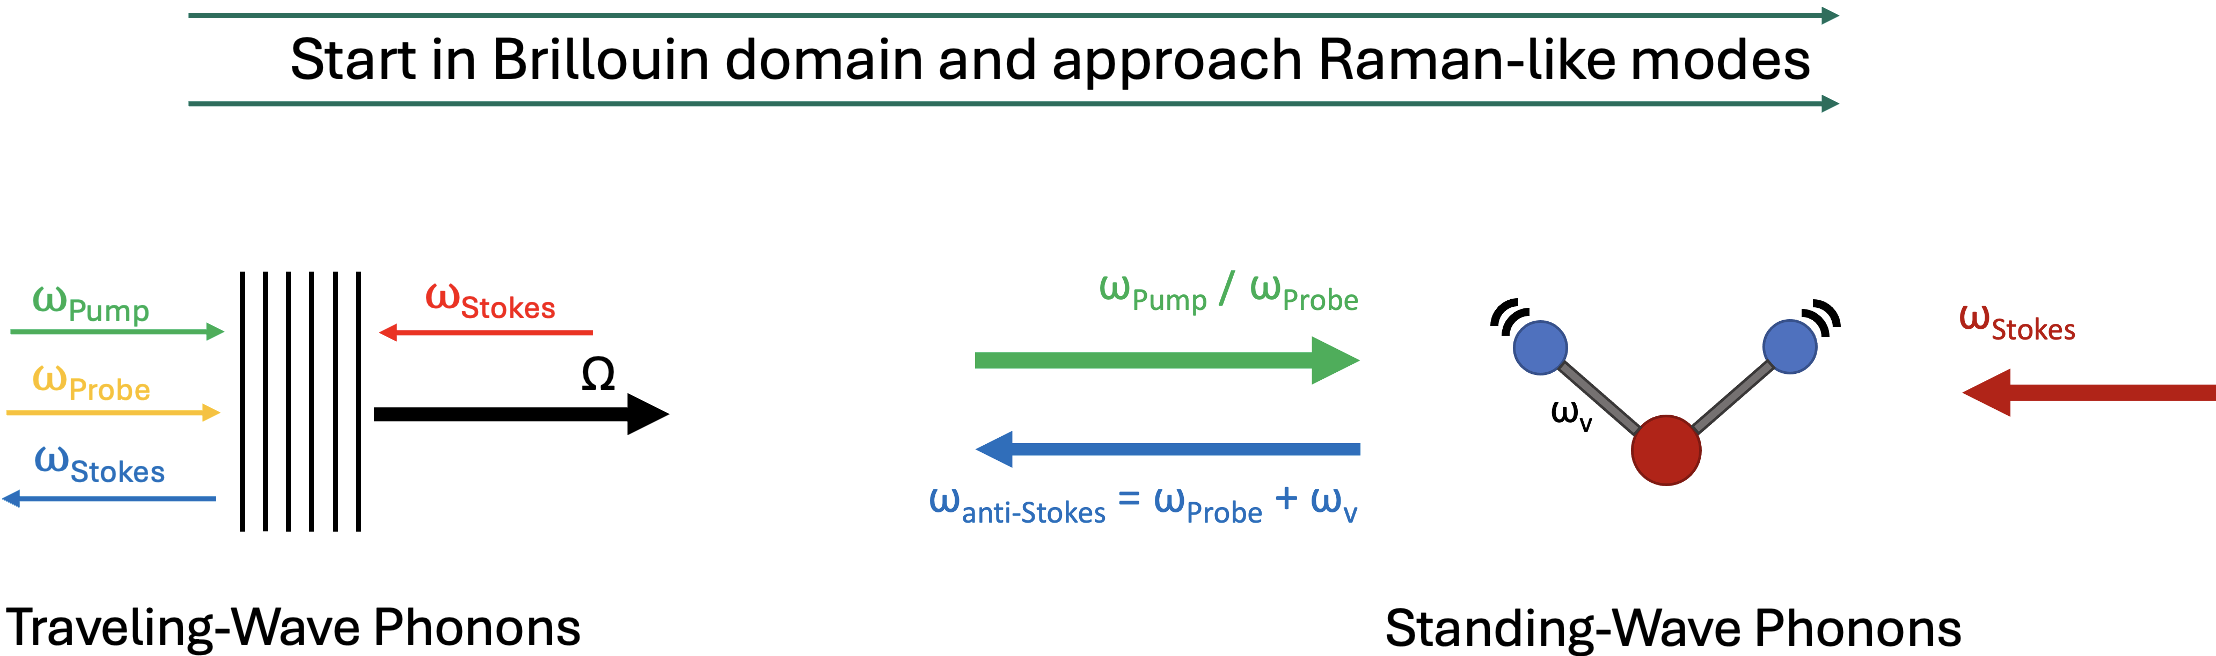
\includegraphics[width=\textwidth]{figs/4-Raman/ExploreBrillouinRamanTransition.png}
  \vspace{0.5em}
  \caption{Conceptual illustration of the transition from a traveling acoustic wave to standing-wave vibrational modes. In a bulk material (left), light scatters from a continuum of (traveling) acoustic waves (Brillouin scattering), whereas in the molecular vibrations of atomic bonds (right), only discrete (standing-wave) phonon modes are allowed. The left diagram is a conceptual visualization of the \ac{CoBS} process for a longitudinally-traveling phonon \(\Omega\) while the right diagram gives a conceptual visualization of an analogous coherently stimulated anti-Stokes Raman scattering process \ac{CARS} with the standing-vibrations \(\omega_{\rm v}\) among bonded atoms in a molecule.}
  \label{fig:Raman:BrillouinRamanTransition}
\end{figure}

\subsection{Brillouin-Induced Raman Modes}
\label{subsec:Raman:Brillouin-InducedRamanModes}

In a traditional SBS experiment, a pump laser drives an acoustic wave through electrostriction, and the scattered Stokes light is down-shifted by the acoustic frequency \(f_{\rm B}\). In an unbounded or long medium, \(f_{\rm B}\) is determined by material properties (sound speed and optical dispersion) and the acoustic wave can be thought of as a traveling grating moving through the medium. If the medium is shortened such that the acoustic wave can reflect off the sample boundaries, the traveling acoustic wave can auto-interfere with itself to form a standing-wave pattern in the medium. Under these system conditions, a phonon induced by \ac{SBS} will propagate to the sample end, reflect (assuming a high acoustic impedance mismatch at the boundary), and traverse the medium in the reverse direction. If the length \(L\) between acoustic interfaces is a half-integer number of acoustic wavelengths, the forward and backward phonon waves can interfere to form a standing wave pattern (i.e., a resonance), in essence trapping the traveling phonon in the cavity defined by the sample. This standing wave in turn acts like a stable grating, enhancing the scattering of light at well-defined frequencies corresponding to its resonances. We term these resonant phonon excitations “Brillouin-induced Raman modes” to reflect their hybrid character.

In more concrete terms, the finite-length system behaves like an acoustic Fabry–Pérot cavity. For a longitudinal acoustic mode, the condition for a standing wave is that an integer number \(n\) of half-wavelengths equals the round-trip length: \(n \cdot (\lambda_{\rm s}/2) = L\). Equivalently, the allowed acoustic frequencies are

\begin{equation}
  f_{\rm n} = \frac{n\,v_{\rm s}}{2L},
  \label{eq:Raman:f_R}
\end{equation}
\\
where \(v_{\rm s}\) is the sound velocity in the medium and \(n = 1, 2, 3, \dots\) indexes the mode order. The lowest-frequency mode (\(n = 1\)) has a fundamental frequency \(f_{\rm 1} \approx v_{\rm s}/(2L)\), and higher modes are integer multiples of this fundamental (assuming a simple one-dimensional confinement). Thus, instead of a single Brillouin shift \(f_{\rm B}\), one expects a ladder of equally spaced phonon modes in the scattering spectrum, resembling a Raman vibrational progression. The spacing \(\Delta f\) between adjacent modes is approximately \(\Delta f \approx v_{\rm s}/(2L)\), set solely by the cavity length and sound speed. Figure~\ref{fig:Raman:GeometryDeterminesFundamentalFreq} illustrates why this is so,  For example, if \(L =\) \SI{10}{\milli\meter} in a medium where \(v_{\rm s} =\) \SI{5000}{\meter\per\second}, the fundamental mode would be \(f_{\rm 1} \sim\) \SI{250}{\kilo\hertz} and overtones at \SI{500}{\kilo\hertz}, \SI{750}{\kilo\hertz}, etc. In principle, a sufficiently short and high-Q acoustic cavity could produce a comb of multiple \si{\giga\hertz}-range lines (analogous to molecular vibrational Raman lines) out of what would ordinarily be a single broad Brillouin gain peak.

\begin{figure}[t]
  \centering
  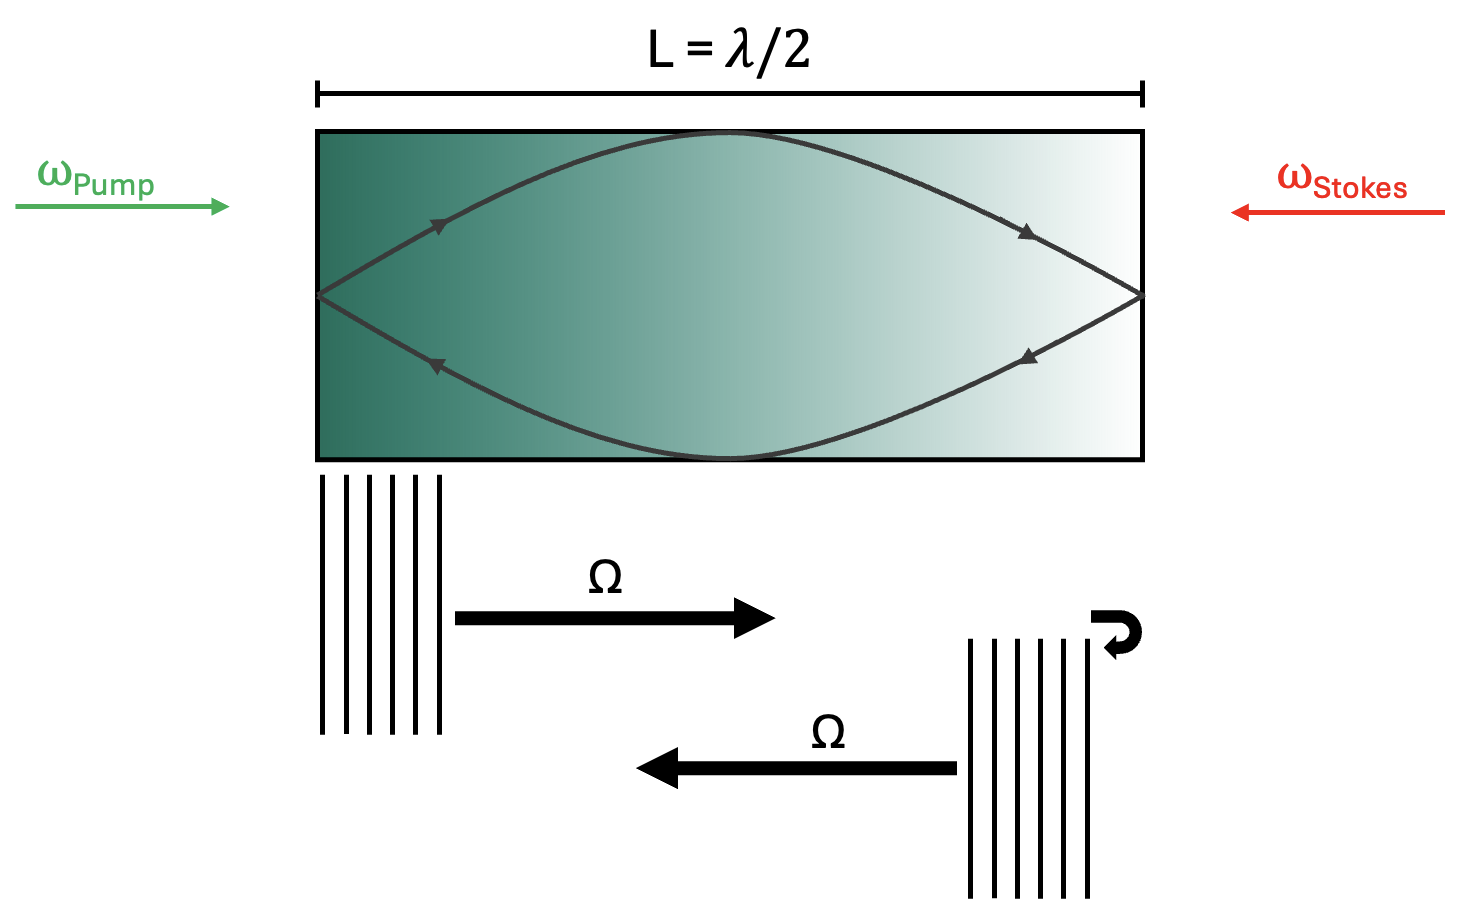
\includegraphics[width=.85\textwidth]{figs/4-Raman/GeometryDeterminesFundamentalFreq.png}
  \caption{Illustration showing how geometry and sound speed of the material determine the allowed acoustic frequencies, given by Equation~\ref{eq:Raman:f_R}. Traveling-wave phonons around the material's Brillouin frequency shift \(f_{\rm B}\) are transduced within the medium via the \ac{CoBS} process. These phonons traverse the length to reach the boundary, where a high acoustic impedance mismatch causes them to reflect at the interface and retraverse the length of the medium in the reverse direction. The spatio-temporal overlap of counterpropagating traveling-wave phonons causes them to interfere, creating an acoustic standing-wave pattern within the material at discrete frequencies determined by the length and sound speed of the material. Shown in the illustration is the half-wavelength fundamental (\(n=1\)) mode, however in general, harmonics near the material's mechanical resonance frequency \(f_{\rm B}\) would be excited in the medium.}
  \label{fig:Raman:GeometryDeterminesFundamentalFreq}
\end{figure}

These Brillouin-induced modes would manifest as distinct peaks in the spectrum of the scattered light. In addition to the usual broadened Brillouin spectrum (with width given by acoustic damping), one would see a series of sharp lines at \(f_{\rm 1}, f_{\rm 2}, f_{\rm 3}, \dots\) around the center scattered frequency. Such a spectrum would be clear evidence that the phonon field is not only a freely propagating wave but also oscillating in discrete standing patterns (i.e., an optically driven acoustic resonator within the material). This is conceptually similar to stimulated Raman scattering in a molecule, where one can get a cascade of Stokes lines corresponding to \(1\hbar\omega_{\rm vib}\), \(2\hbar\omega_{\rm vib}\), \(3\hbar\omega_{\rm vib}\) energy shifts if the pump is intense. Here the “molecular vibration” is replaced by an acoustic cavity mode. If the pump power is high enough to drive the acoustic mode into the nonlinear regime, one might even observe multiple orders of Stokes (and anti-Stokes) as the phonon population builds up in those modes.

The idea of \ac{SBS}-driven acoustic modes has parallels in prior work. In the cryogenic experiment of Renninger et al. mentioned earlier, \cite{renninger2018bulk} a bulk acoustic mode was driven via Brillouin scattering in a \si{\centi\meter}-scale quartz crystal. At low temperatures, they observed ultra-narrow acoustic resonances (indicative of discrete modes) in place of a broad Brillouin response, confirming that acoustic coherence across the entire sample can indeed produce a modal spectrum. In our case, we seek to do this at room temperature by engineering a shorter effective acoustic cavity. We aim to accomplish this by taking advantage of our Coherently Stimulated Brillouin Spectrometer (\ac{CoBS}), which offers \(\sim10^{6}\) improvement in scattered power for \(\sim\)\si{\centi\meter} lengths over traditional \ac{SBS} (see Appendix~\ref{appendix:comparison} for a comparison of scattered power across Brillouin techniques, and specifically Figure~\ref{fig:SponBSvsStimBSvsCoBS} for a comparison by effective length \(L\)).

\subsection{Key Parameters and Feasibility}
\label{subsec:Raman:KeyParametersandFeasibility}

Observing Raman-like standing-wave modes via \ac{SBS} hinges on several key parameters of the system. We identify three especially critical factors: (1) the scattered power, determined by the effective material Brillouin gain and length as well as the optical powers; (2) the acoustic dissipation in the medium, which limits the mean phonon travel distance; and (3) the acoustic boundary reflectivity, determined by impedance mismatch at interfaces, which enables the phonons to reflect and form standing-waves. These parameters together determine whether the phonon will remain a distributed traveling excitation or collapse (blur) into discrete modes. Chapter~\ref{ch:CoBS} describes the \ac{CoBS} instrument, showing that the scattered power as a result of the \ac{CoBS} process is given by Equation~\ref{Eq:Theoretical Framework:Scattered Power}, stated here again as

\begin{equation}
  P_{\rm Signal} = \frac{1}{4}(G_{\rm B}L)^{2}P_{\rm Pump}P_{\rm Stokes}P_{\rm Probe}\Phi,
  \label{eq:Raman:ScatteredPowerPhi}
\end{equation}
\\
where \(G_{\rm B}\) is the material-dependent effective (acousto-optic overlap-adjusted) Brillouin gain factor given by Equation~\ref{Eq:Effective Brillouin Gain}, \(L\) is the effective length, \(P_{\rm i}\) are the optical powers of the pump, Stokes, and probe waves, respectively, and \(0 < \Phi < 1\) is a phase-matching relaxation term (given by Equation~\ref{Eq:Phi}) that captures the pump-probe detuning on which the instrument relies. A material’s Brillouin gain coefficient \(g_{\rm 0}\) (\si{\watt\per\meter}), or overlap‐adjusted effective gain \(G_{\rm B}\) (\si{\per\watt\per\meter}), sets how strongly the phonons are driven for given pump \(P_{\rm P}\), Stokes \(P_{\rm S}\), and probe \(P_{\rm Pr}\) optical powers over an interaction length \(L\) in the \ac{CoBS} process (see Chapter~\ref{ch:CoBS}, and specifically Equation~\ref{Eq:Theoretical Framework:Scattered Power}), given here again by

\begin{equation}
  G_{\rm B} = \frac{g_{0}}{A_{\rm eff}}\frac{\left(\frac{\Gamma_{\rm B}}{2}\right)^{2}}{\left(\Omega - \Omega_{\rm B}\right)^{2} + \left(\frac{\Gamma_{\rm B}}{2}\right)^{2}}.
  \label{eq:Raman:GB}
\end{equation}
\\
Here, \(\Gamma_{\rm B}\) is the angular Brillouin linewidth, \(\Omega\) (\(\Omega_{\rm B}\)) is the (resonant) angular acoustic frequency, \(A_{\rm eff}\) is the effective area (acousto-optic mode overlap), and \(g_{0}\) is the Brillouin gain coefficient given by

\begin{equation}
  g_{0} = \frac{\gamma_{\rm e}^{2}\omega^{2}}{nv_{\rm s}c^{3}\rho_{0}\Gamma_{\rm B}},
  \label{eq:Raman:g0}
\end{equation}
\\
where \(\gamma_{\rm e}\) is the electrostrictive constant, \(\omega\) is the angular optical frequency, \(n\) is the refractive index, \(v_{\rm s}\) is the speed of sound in the material, \(c\) is the speed of light, and \(\rho_{0}\) is the mean density of the material. Short samples demand very high effective Brillouin gain to achieve significant scattered power in a small \(L\). Certain tellurium‐based materials, for instance, can offer gains orders of magnitude higher than silica, \cite{sanghera2010nonlinear, abedin2005observation} allowing measureable scattered power in sub‐\si{\milli\meter} cavities.

Even if phonons are driven strongly, they must live long enough (i.e., have a low enough dissipation rate, or high enough acoustic Q) to form a standing wave. At room temperature, intrinsic damping can limit phonon \(Q_{\rm s}\) to \(\sim10^{3}\)–\(10^{4}\) in many solids, \cite{heiman1979brillouin, bucaro1974high} implying attenuation lengths of \si{\milli\meter} to \si{\centi\meter} for \si{\giga\hertz} frequencies. Ideally, the sample length \(L\) should be comparable to or less than half the attenuation length so that phonons undergo multiple round trips. This is considerably more difficult at room temperature than at cryogenic temperatures, where \(Q_{\rm s}\) can exceed \(10^{7}\). \cite{maris1990phonon, renninger2018bulk} Finally, the phonon must reflect rather than escape at the boundaries. A large acoustic impedance mismatch (e.g., a free surface with air on one side) can approach nearly 100\% reflection. \cite{galliou2013extremely, auld1973acoustic} Designing the sample with two opposing highly acoustically reflective boundaries is essential to generating a Raman-like standing-wave mode in the medium. In practice, however, partial reflections at each (or even just one) end can suffice so long as the net round‐trip reflectivity is high enough to sustain a mode.

In short, we want to create a high-\(Q\) acoustic resonator inside a Brillouin-active medium at room temperature: strong enough acousto-optic driving to excite the phonons, low enough damping to maintain them, and robust boundary reflections to confine them. Meeting all of these conditions can be challenging. However, the high (\(\sim\)\SI{5}{\femto\watt}) sensitivity and unique short path length advantage of our \ac{CoBS} instrument (described in Chapter~\ref{ch:CoBS} and Section~\ref{appendix:comparison}) sparks new motivation, as it provides a new technique tailored for observing small-scale scattering phenomenon. Feasibility estimates and initial \ac{CoBS} measurements indicate that by utilizing ultra-high-gain media such as \ce{Te} \cite{sanghera2010nonlinear, abedin2005observation} or liquid \ce{CS2} \cite{boyd2020nonlinear}, and ensuring at least one boundary is acoustically reflective, one can push toward Brillouin-induced Raman modes even under ambient conditions.

The sensitivity of our instrument, representing the minimum scattered power that may be detected, has been measured at \(P_{\rm Signal}\approx\) \SI{5}{\femto\watt} (see Section~\ref{Results:Instrument sensitivity}, and specifically Table~\ref{tab:CoBS:5fWSensitivity} together with Equation~\ref{Eq:Theoretical Framework:Scattered Power} and Figure~\ref{fig:CoBS:5fWSensitivity} for validation of this claim). Using this sensitivity value for \(P_{\rm Signal}\) we can rearrange Equation~\ref{eq:Raman:ScatteredPowerPhi} to solve for the minimum length \(L\) we can expect to observe scattering within for given optical powers, material gain, and pump-probe detuning:

\begin{equation}
  L = \frac{2}{G_{\rm B}}\sqrt{\frac{P_{\rm Signal}}{P_{\rm Pump}P_{\rm Stokes}P_{\rm Probe}\Phi}},
  \label{eq:Raman:minimumL}
\end{equation}
\\
where \(0 < \Phi < 1\) and increases for smaller \(L\). For \(P_{\rm Signal}\approx\)\SI{5}{\femto\watt} sensitivity and maximum optical powers \(P_{\rm Pump}P_{\rm Stokes}P_{\rm Probe}=\) \SI{0.25}{\cubic\watt} under typical conditions, Equation~\ref{eq:Raman:minimumL} predicts, for example, the ability to observe scattering within \(\sim\)\SI{500}{\nano\meter} of \ac{UHNA3} fiber (\(G_{\rm B,\,UHNA3}=\) \SI{0.6}{\per\watt\per\meter}). Equation~\ref{eq:Raman:minimumL} makes clear that minimizing the observable scattering length is accomplished by any of: bumping optical powers, improving instrument sensitivity, or choosing a higher gain scattering medium.

In what follows, we detail the experimental platforms and theoretical modeling that guided our attempts to observe discrete phonon modes in high-gain materials. Although a conclusive demonstration proved elusive, the conceptual framework is robust and provides a foundation for ongoing efforts. By shrinking the acoustic path length, maximizing phonon reflectivity, and exploiting strong \ac{CoBS} gain, one can approach the regime where traveling-wave Brillouin scattering morphs into Raman-like standing-wave modes. This pursuit effectively unifies the traveling-wave and standing-wave paradigms of light-sound interaction, providing new opportunities in cavity-free phononics, resonant optomechanics, and coherent phonon devices at room temperature.

\begin{figure}[t]
  \centering
  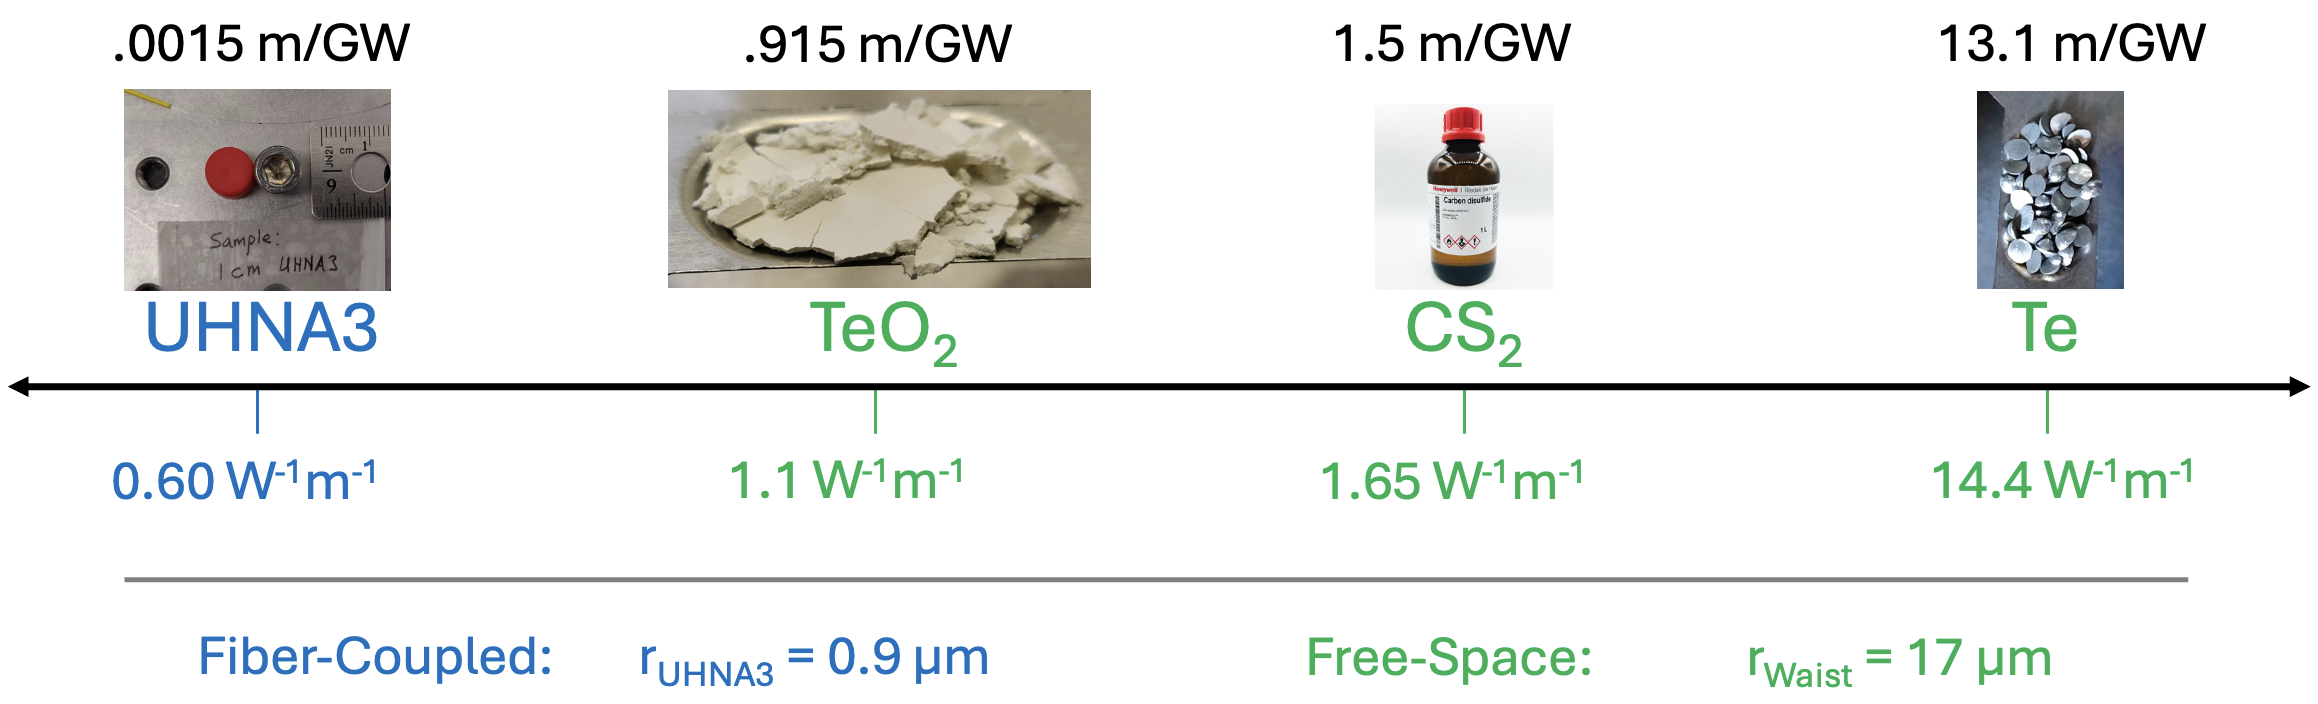
\includegraphics[width=\textwidth]{figs/4-Raman/GainOfRelevantMaterials.png}
  \caption{Gain of relevant materials.}
  \label{fig:Raman:GainOfRelevantMaterials}
\end{figure}

%--------------------------------------------------------------------%

\section{Results}
\label{sec:Raman:Results}

Plots
\begin{itemize}
  \item UHNA3 - 1cm, 1mm
  \item CS2 vial - 4mm, 2mm
  \item TeO2 films - 1um, 500nm
  \item CS2 - 1mm, 100um, (10um not quite)
  \item chip waveguide - chip/nochip, holes
\end{itemize}

\subsection{Germanium-Doped Optical Fiber}
\label{subsec:Raman:Target:UHNA3}

\begin{itemize}
  \item 1cm, 1mm
\end{itemize}

\begin{figure}[t]
    \centering
    \begin{subfigure}[b]{0.49\textwidth}
        \centering
        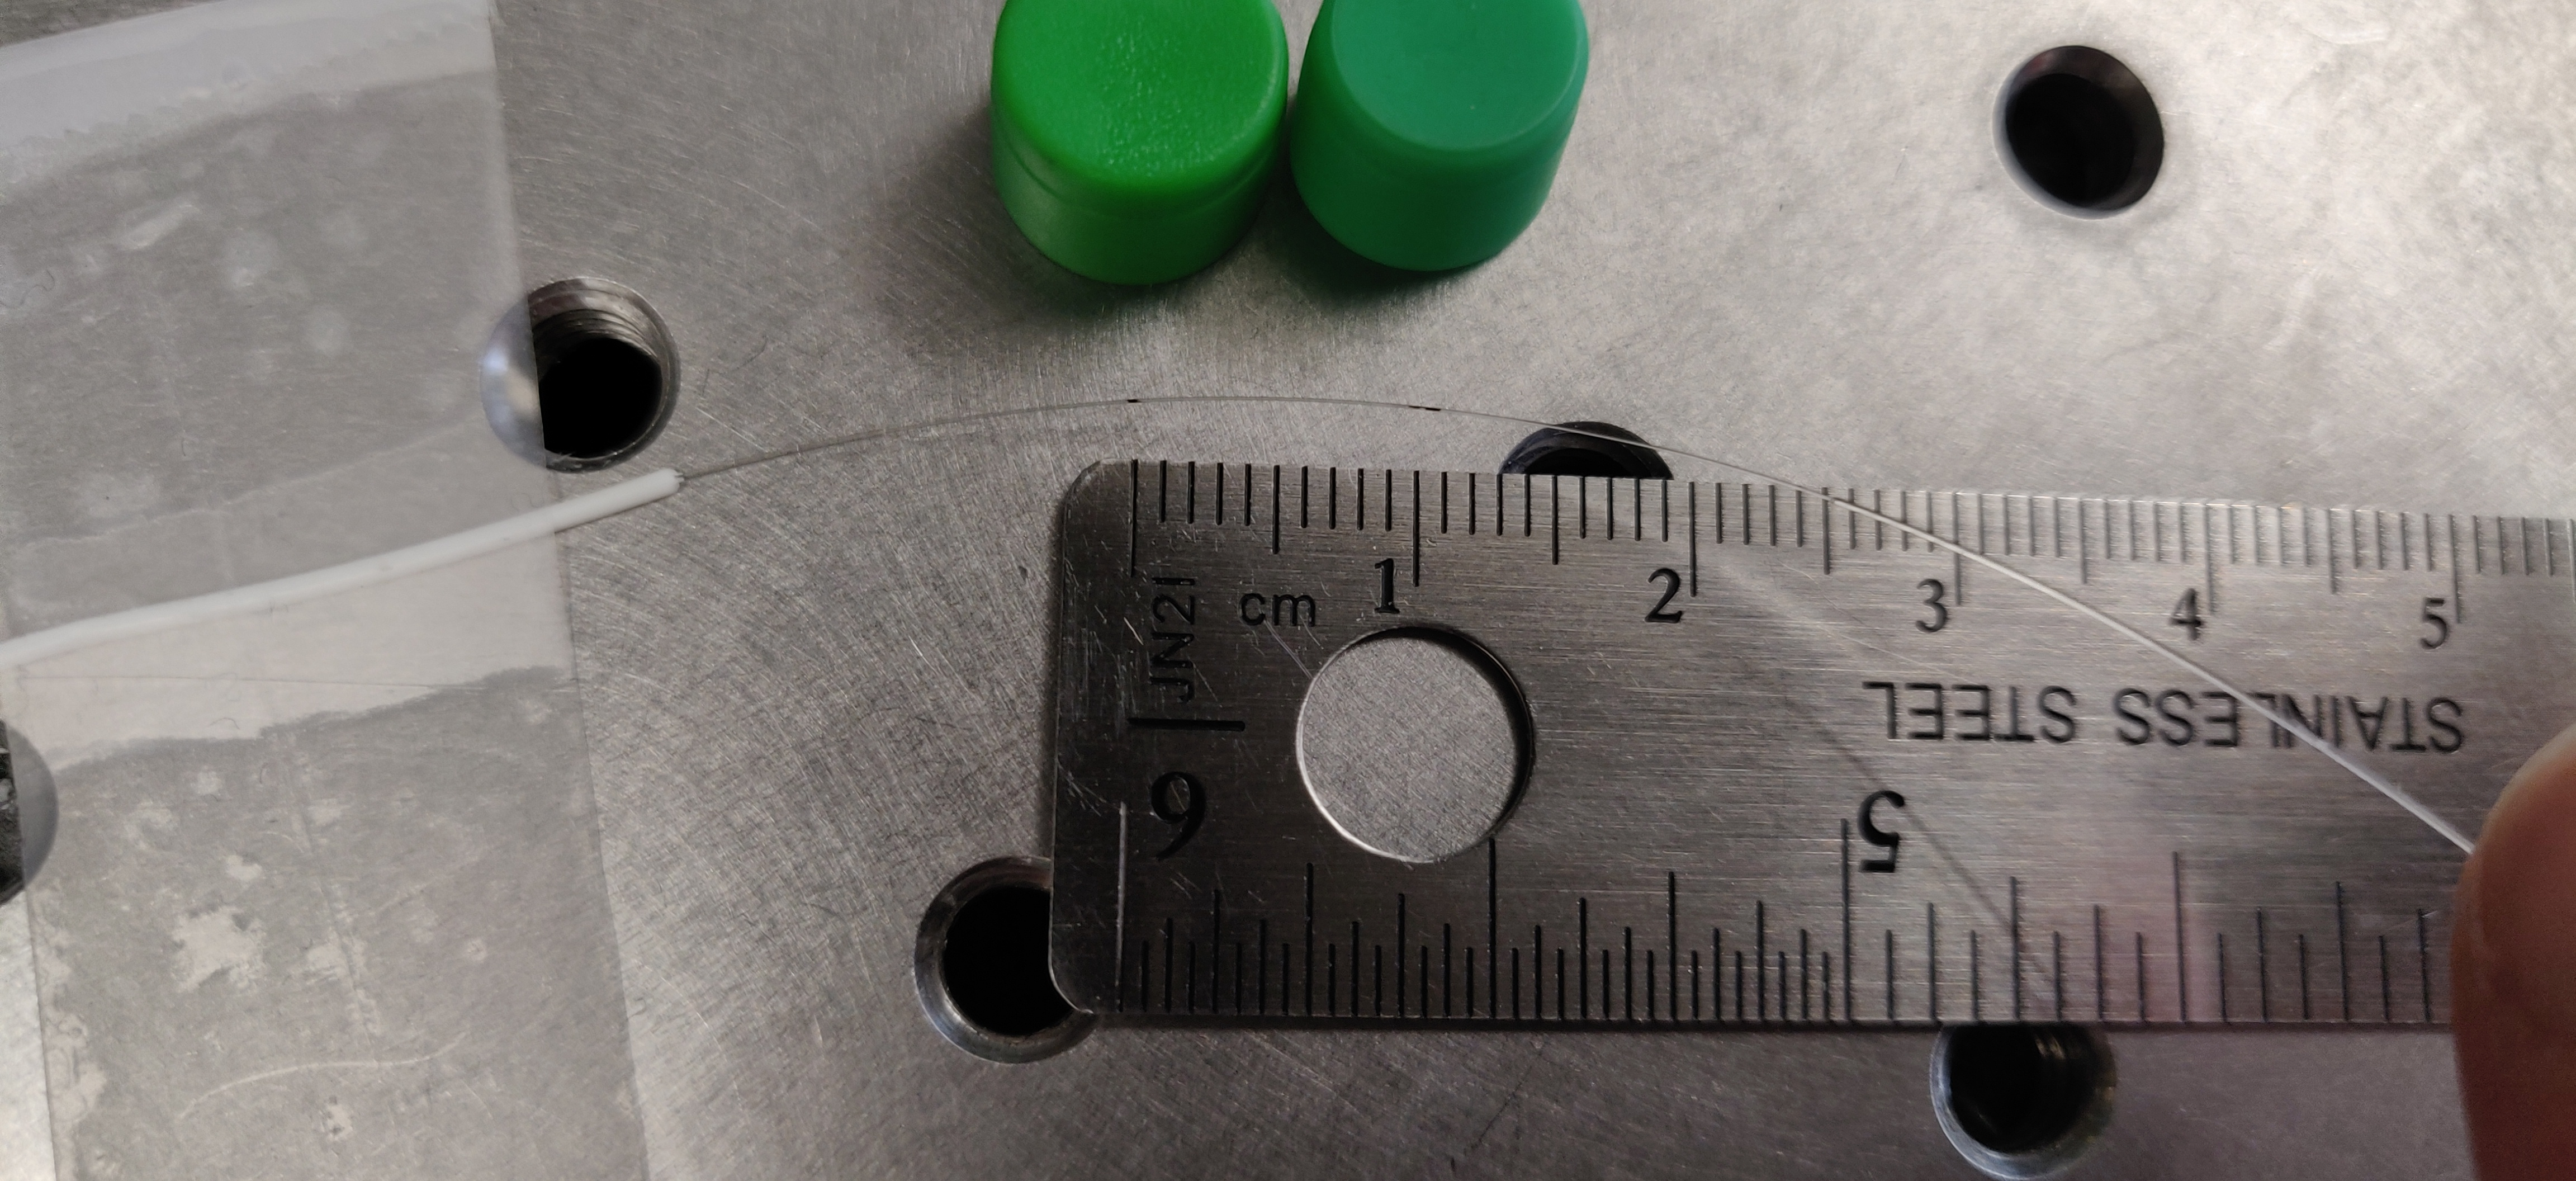
\includegraphics[width=\textwidth]{figs/4-Raman/1cm UHNA3.jpeg}
        \caption{}
        \label{fig:Raman:1cmUHNA3pic}
    \end{subfigure}
    \hfill
    \begin{subfigure}[b]{0.49\textwidth}
        \centering
        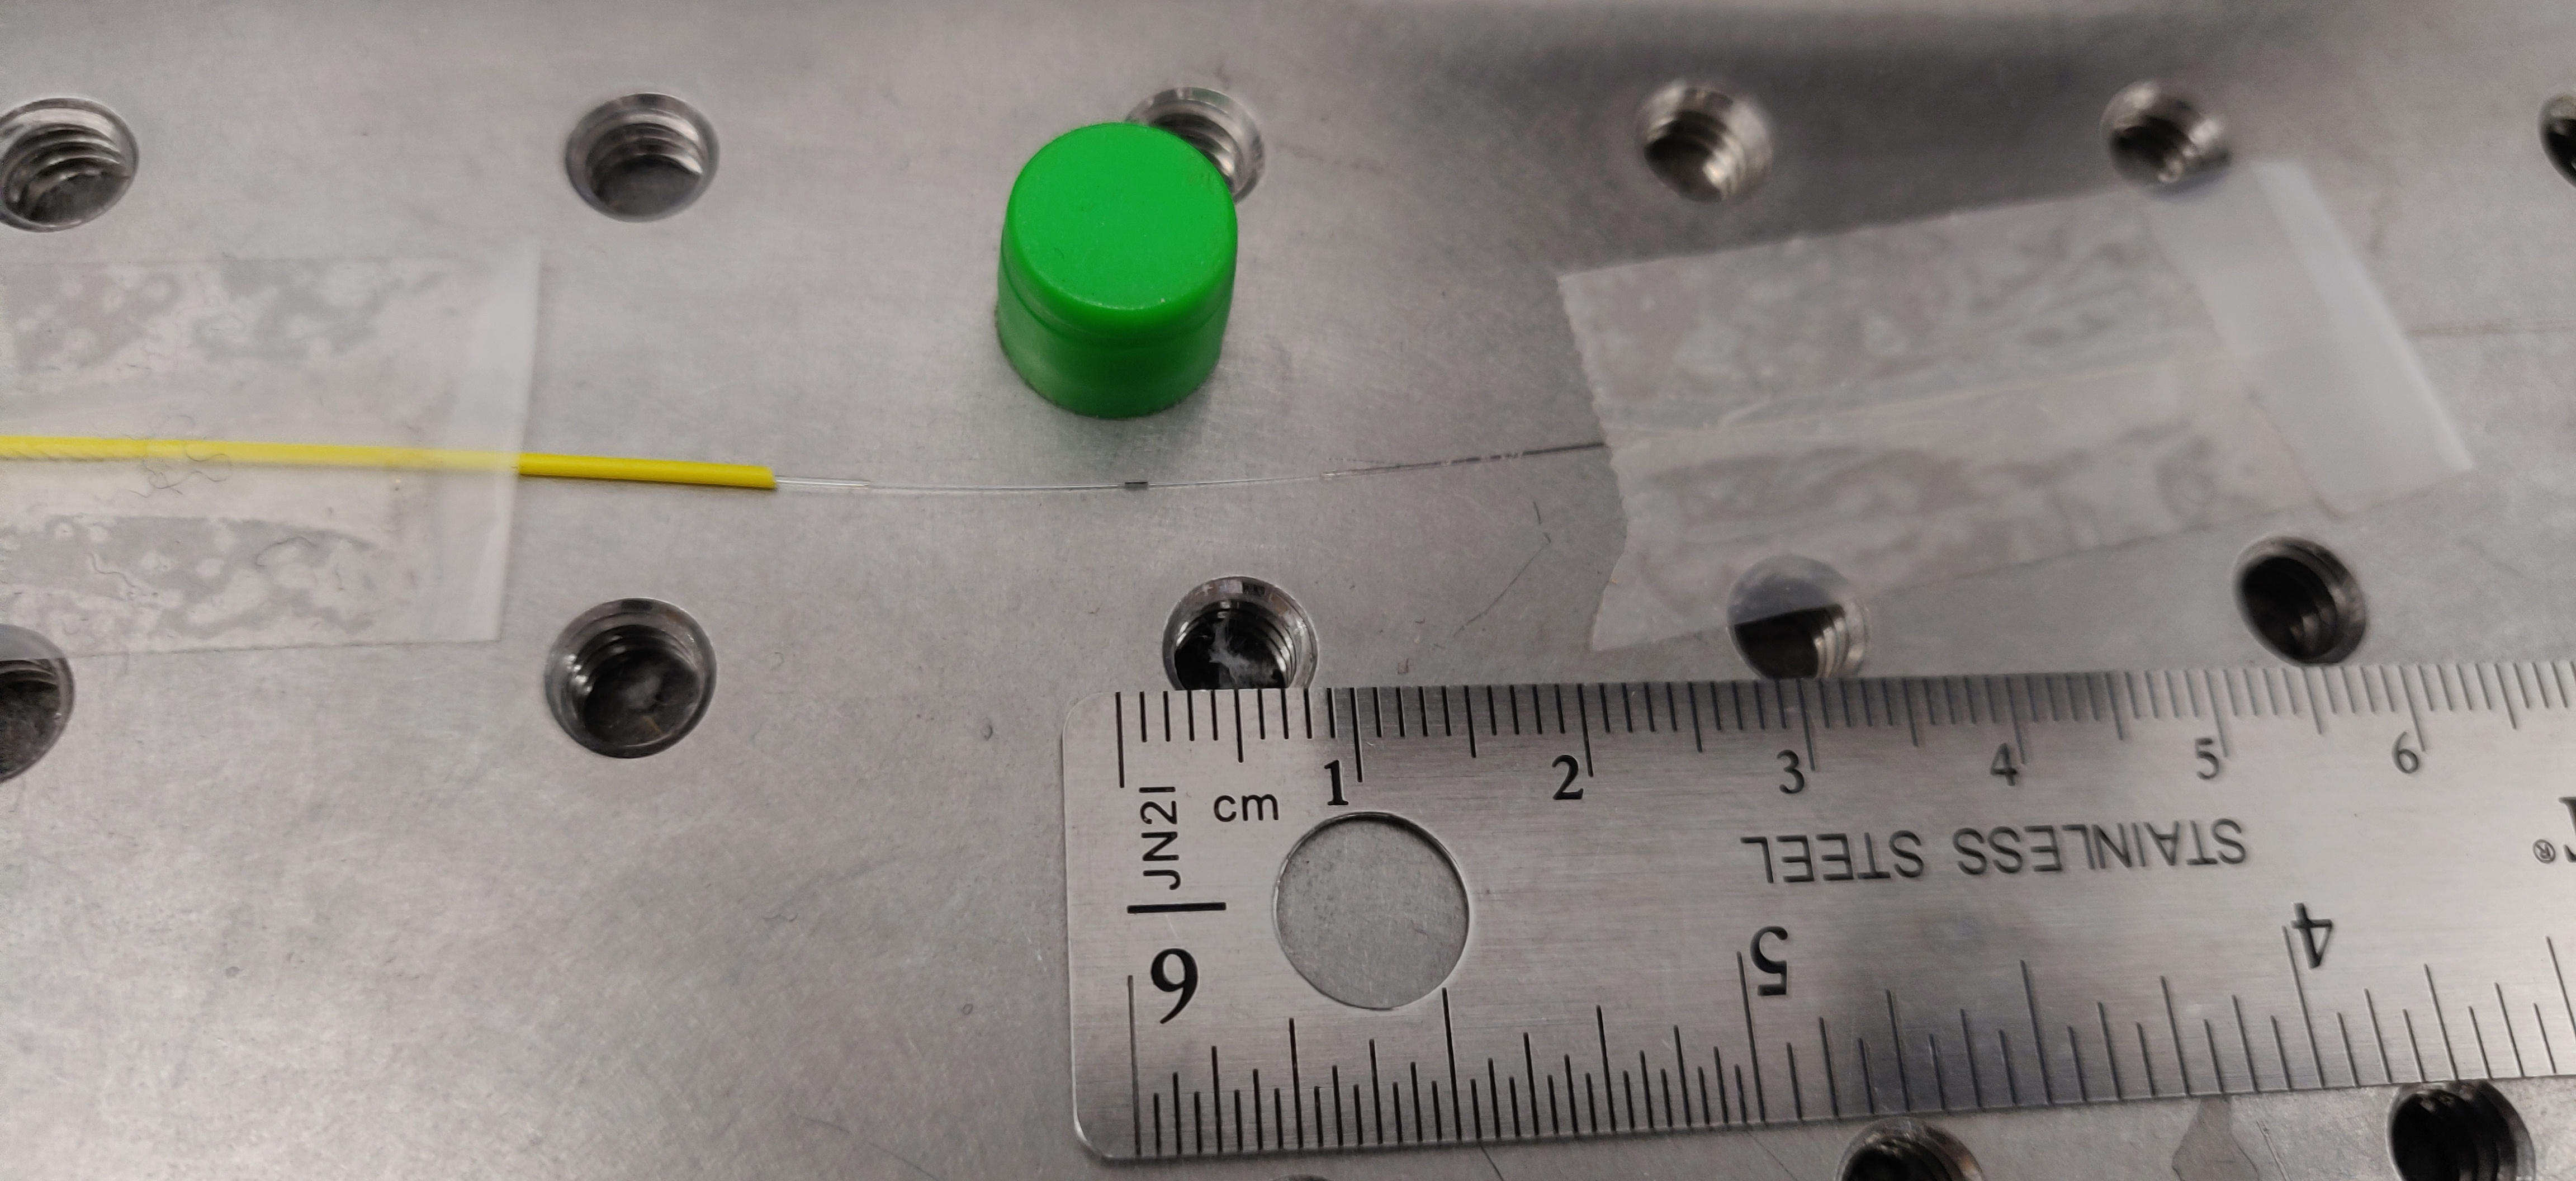
\includegraphics[width=\textwidth]{figs/4-Raman/1mm UHNA3 in apparatus.jpeg}
        \caption{}
        \label{fig:Raman:1mmUHNA3pic}
    \end{subfigure}
    \caption{\SI{1}{\centi\meter} (\ref{fig:Raman:1cmUHNA3pic}) and \SI{1}{\milli\meter} (\ref{fig:Raman:1mmUHNA3pic}) \ac{UHNA3}.}
    \label{fig:Raman:UHNA3}
\end{figure}

\subsection{Free-Space Optics with Liquid Carbon Disulfide}
\label{subsec:Raman:Target:CS2Vial}

\begin{itemize}
  \item Free space with vial
\end{itemize}

\begin{figure}[t]
    \centering
    \begin{subfigure}[b]{0.49\textwidth}
        \centering
        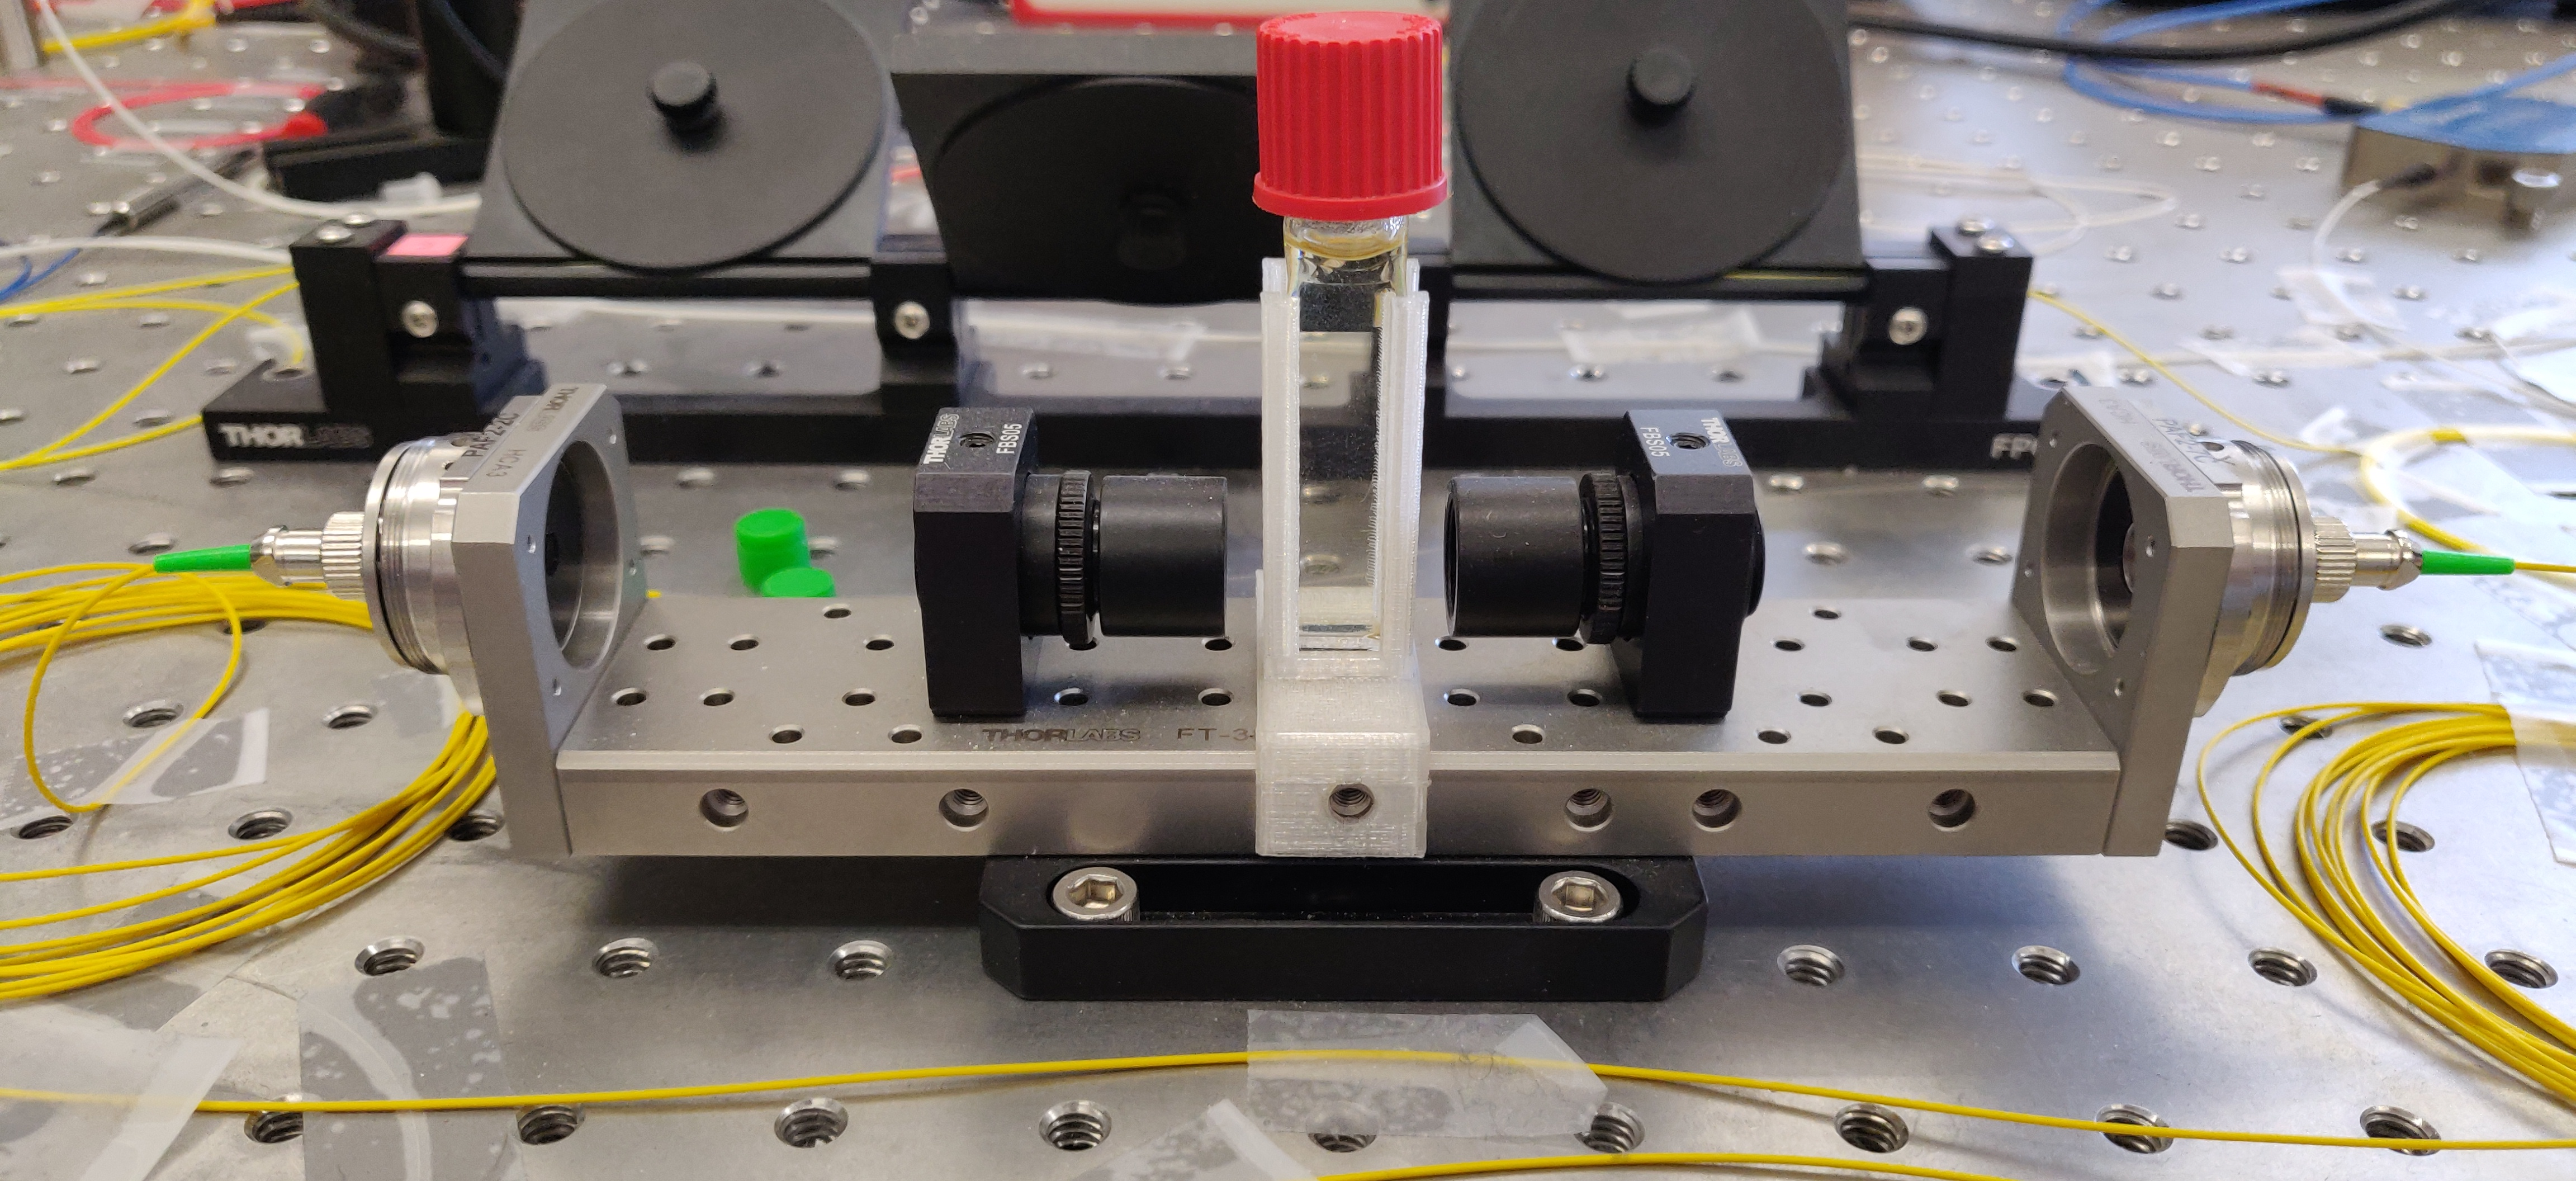
\includegraphics[width=\textwidth]{figs/4-Raman/1cmCS2.jpeg}
        \caption{}
        \label{fig:Raman:1cmCS2}
    \end{subfigure}
    \hfill
    \begin{subfigure}[b]{0.49\textwidth}
        \centering
        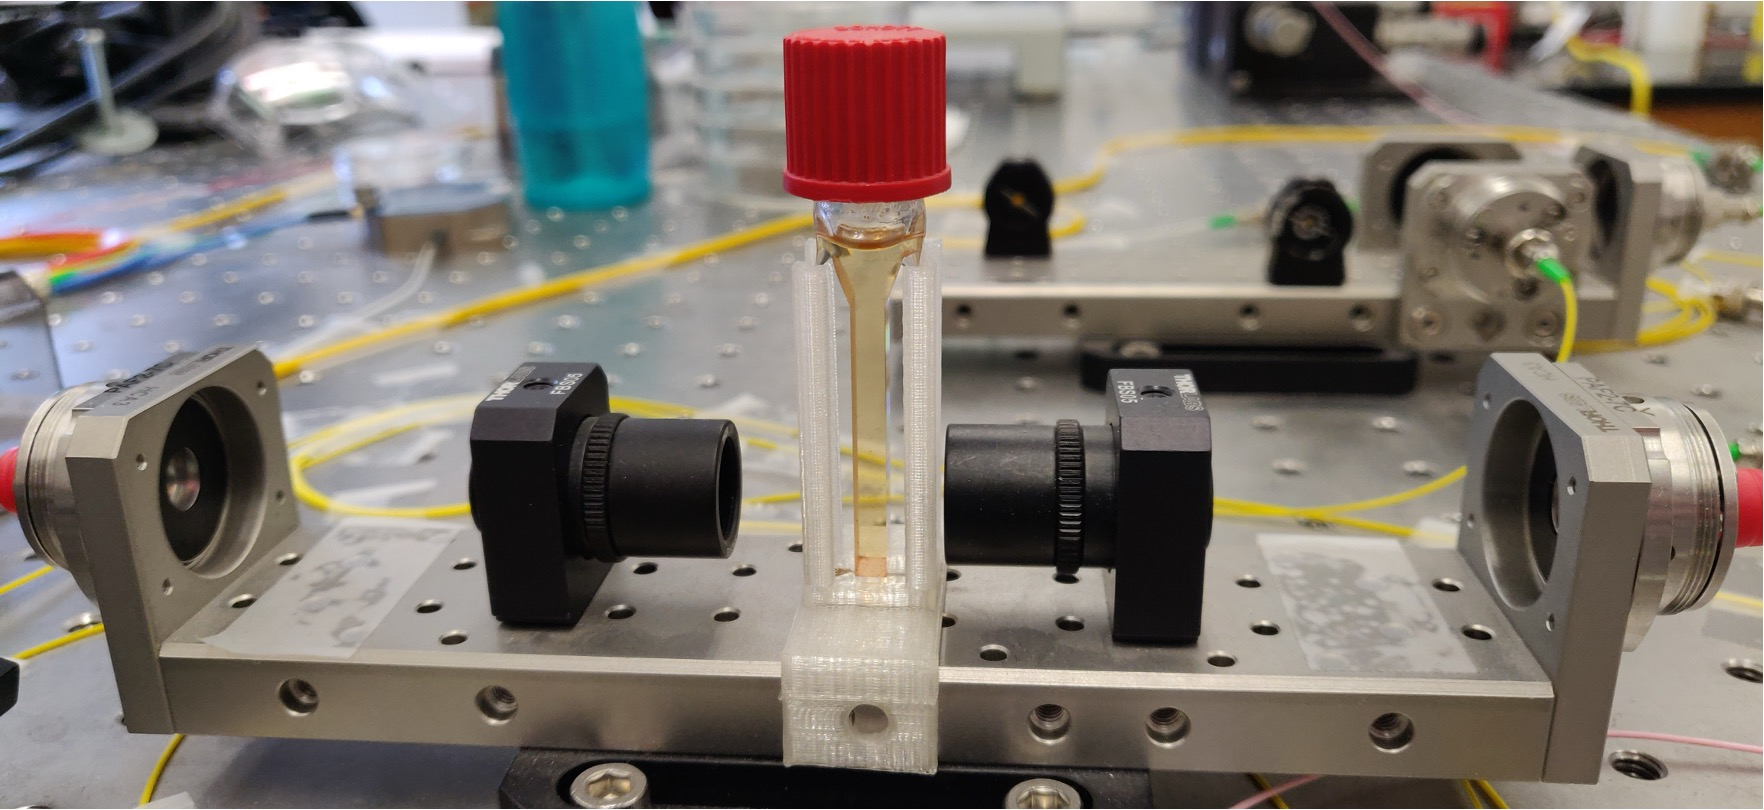
\includegraphics[width=\textwidth]{figs/4-Raman/4mmCS2.jpg}
        \caption{}
        \label{fig:Raman:4mmCS2}
    \end{subfigure}
    \caption{\SI{1}{\centi\meter} (\ref{fig:Raman:1cmCS2}) and \SI{4}{\milli\meter} (\ref{fig:Raman:4mmCS2}) liquid \ce{CS2}.}
    \label{fig:Raman:CS2Cuvet}
\end{figure}

\subsection{Tellurium Dioxide Thin Film}
\label{subsec:Raman:Target:TeO2}

\begin{itemize}
  \item Gibbs collab
  \item deposit Te, oxidize into TeO2
  \item table of relevant TeO2 parameters
\end{itemize}

\subsection{Tellurium Thin Film}
\label{subsec:Raman:Target:Te}

\begin{itemize}
  \item Gibbs collab and CINT collab
  \item oxidizes to TeO2
  \item table of relevant Te parameters
\end{itemize}

\begin{figure}[t]
  \centering
  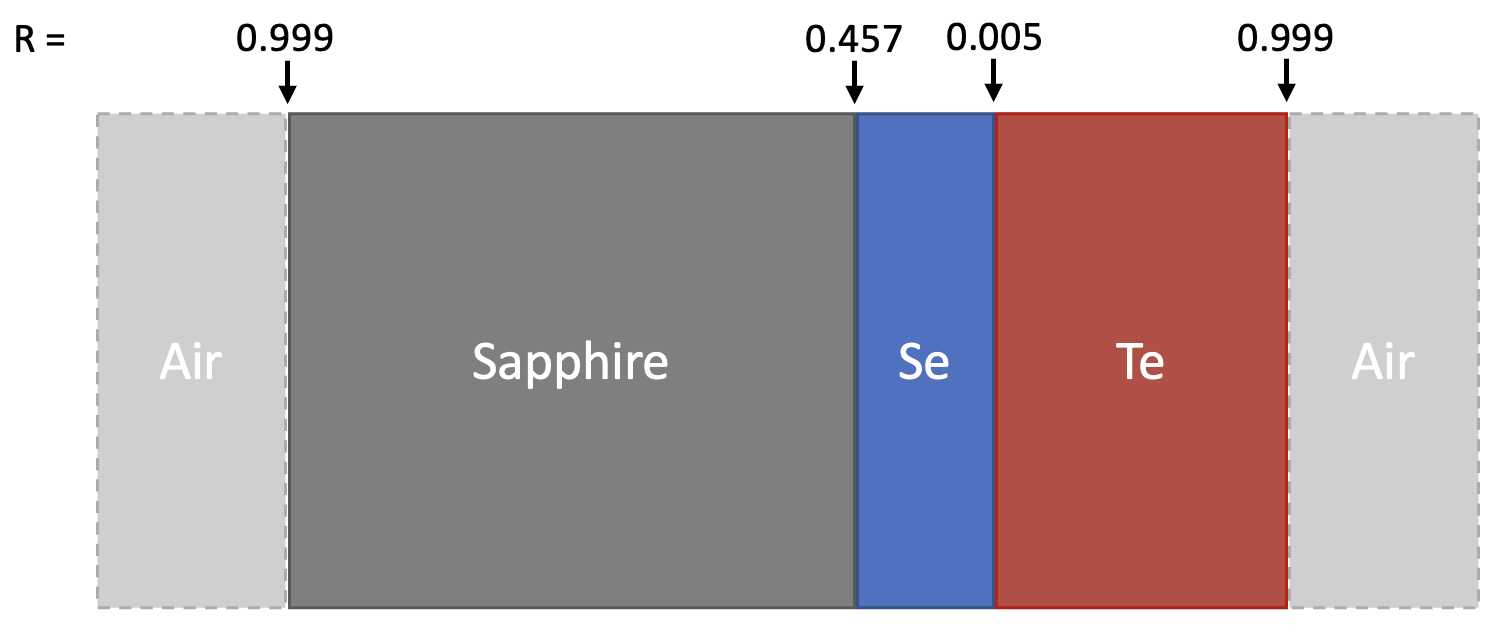
\includegraphics[width=.8\textwidth]{figs/4-Raman/AcousticImpedance.png}
  \caption{Acoustic impedance.}
  \label{fig:Raman:AcousticImpedance}
\end{figure}

\subsection{Carbon Disulfide Micrometer Cell}
\label{subsec:Raman:Target:CS2Cells}

\begin{itemize}
  \item table of relevant CS2 parameters
  \item cells, 1 W amp, bubble test
\end{itemize}

\begin{figure}[t]
    \centering
    \begin{subfigure}[b]{0.3\textwidth}
        \centering
        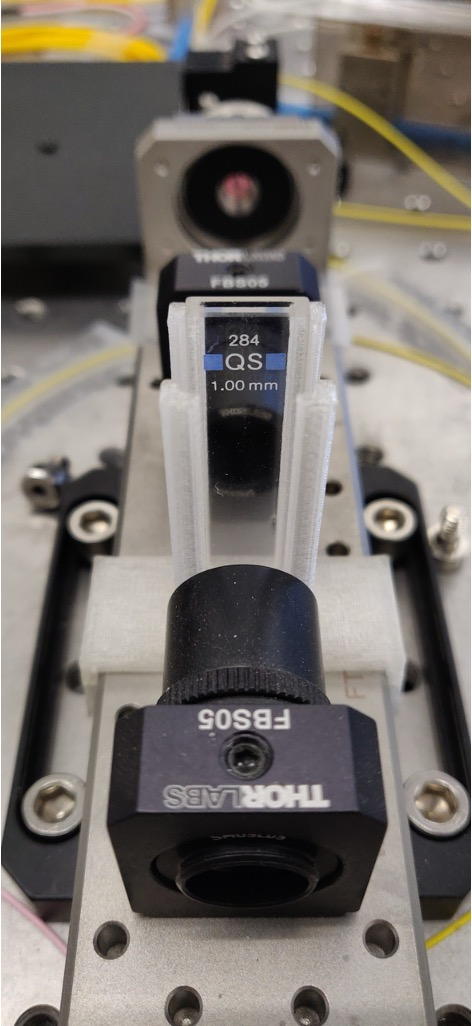
\includegraphics[width=\textwidth]{figs/4-Raman/1mmCS2.jpg}
        \label{fig:Raman:1mmCS2}
    \end{subfigure}
    \hfill
    \begin{subfigure}[b]{0.3\textwidth}
        \centering
        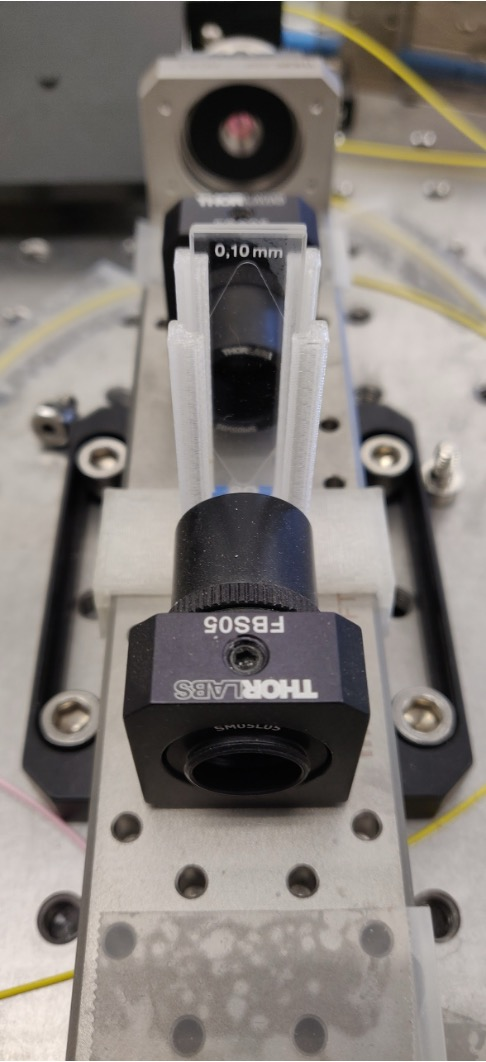
\includegraphics[width=\textwidth]{figs/4-Raman/100umCS2.jpg}
        \label{fig:Raman:100umCS2}
    \end{subfigure}
    \hfill
    \begin{subfigure}[b]{0.3\textwidth}
        \centering
        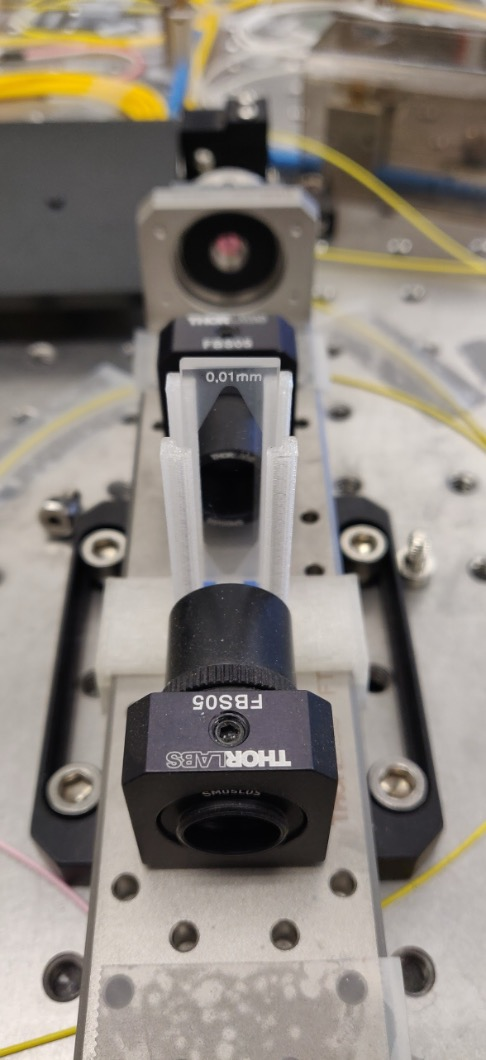
\includegraphics[width=\textwidth]{figs/4-Raman/10umCS2.jpg}
        \label{fig:Raman:10umCS2}
    \end{subfigure}
    %
    \caption{Three \ce{CS2} cells of different path lengths (\SI{1}{\milli\meter}, \SI{100}{\micro\meter}, and \SI{10}{\micro\meter}) secured in the beam path of the \acl{CoBS}.}
    \label{fig:Raman:CS2Comparison}
\end{figure}

\subsection{Suspended Silica Rib Waveguide}
\label{subsec:Raman:Target:Waveguide}

\begin{itemize}
  \item BYU collab
  \item If we can couple chip waveguide into CoBS fiber-chip-fiber, then we have access to a playground of materials and geometries
  \item initial test took 9 months to learn and measure
\end{itemize}

\subsection{Elastically-Suspended Photonic-Phononic Waveguide}
\label{subsec:Raman:Target:WigglyWaveguide}

Figure~\ref{fig:Raman:wigglyCoBSspectra} plots the spectra collected from a \ac{CoBS} measurement of backward Brillouin scattering in the elastically-suspended silica rib of the photonic-phononic waveguide. In this section, we present theoretical estimates of the key mechanical modes and optomechanical couplings predicted for the elastically-suspended photonic-phononic waveguide under development. The structure under consideration consists of a polymeric (SU-8) membrane that is tensioned during high-temperature curing and supports a rib waveguide above it. This combined membrane-and-rib geometry gives rise to multiple distinct mechanical resonances that can be excited and probed optically via the \ac{CoBS} instrument operating in the forwards scattering configuration. We summarize below the principal modes, referred to as ``drumhead'' modes for the membrane and ``breathing'' modes for the rib, and estimate rough frequency ranges in which they are expected to appear.

\begin{figure}[t]
  \centering
  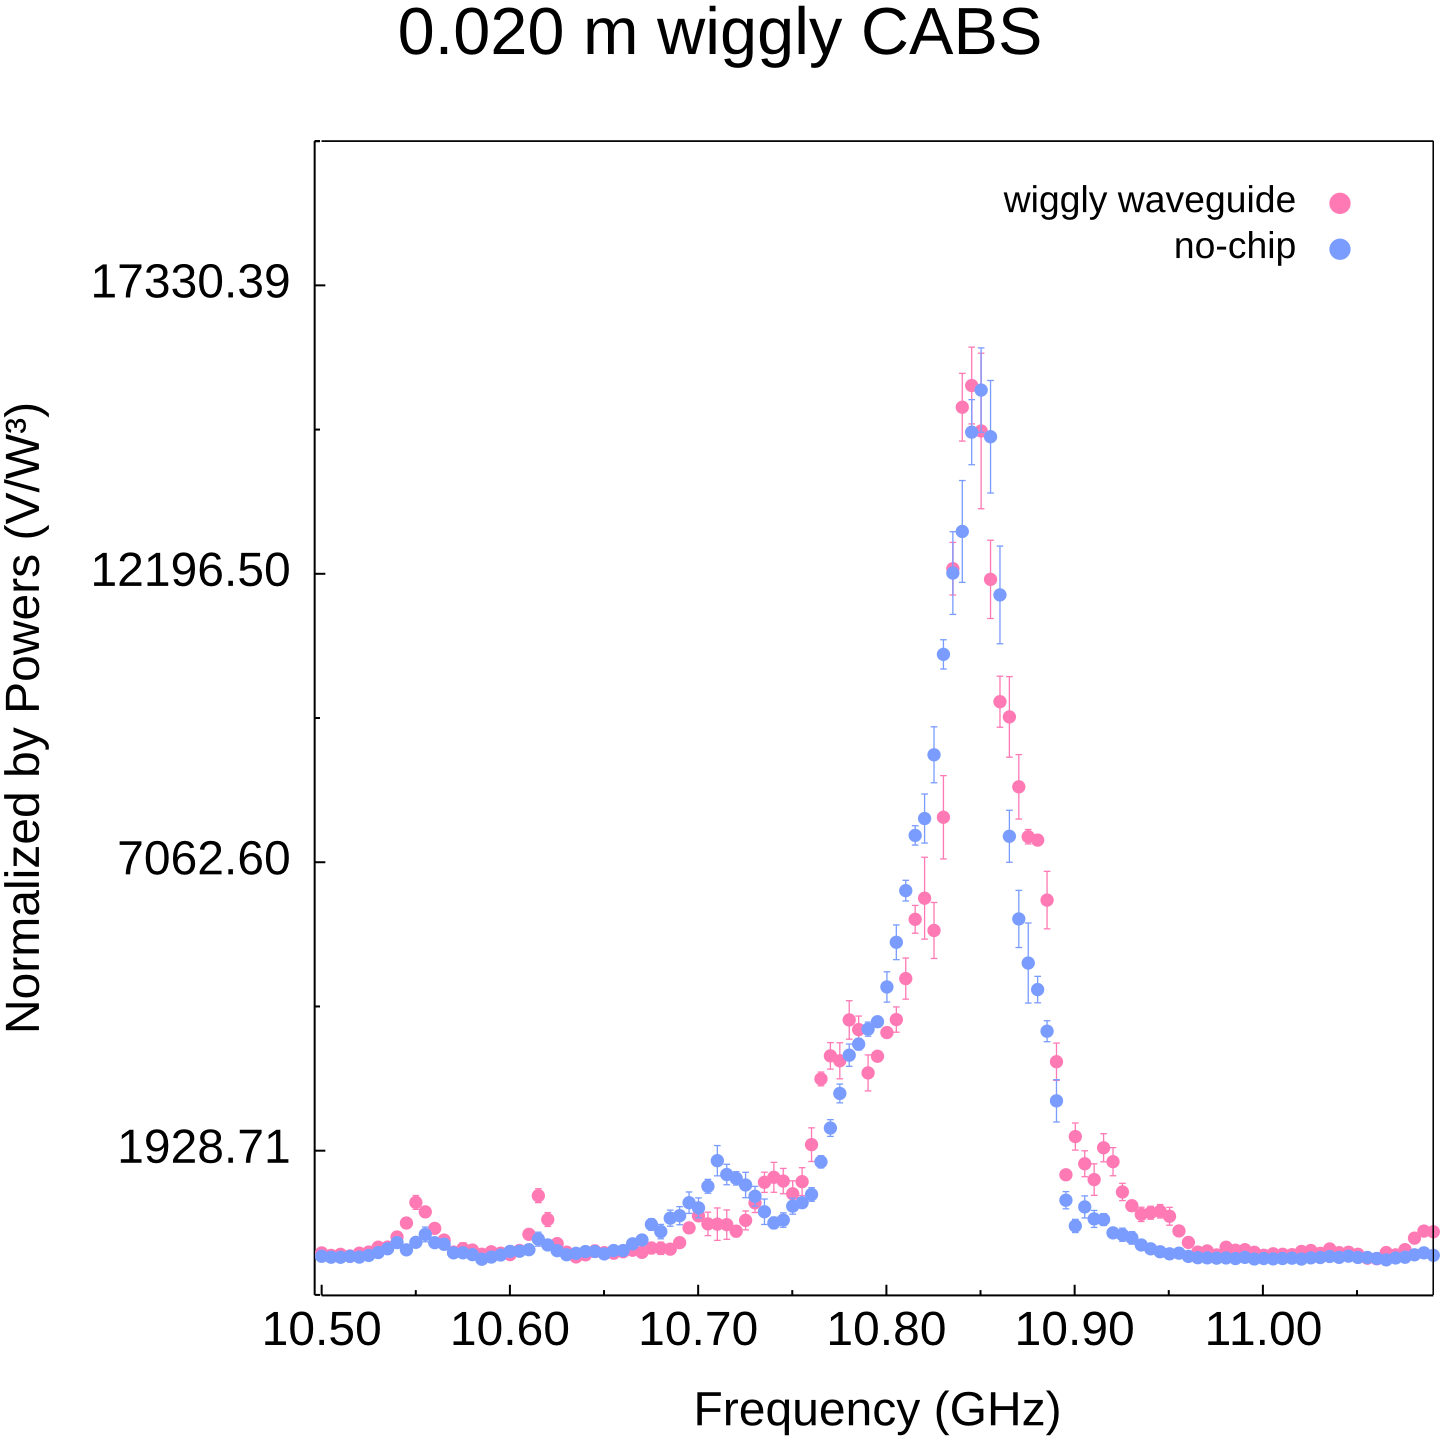
\includegraphics[width=\textwidth]{figs/4-Raman/wigglyWaveguideMeasurement.png}
  \caption{\ac{CoBS} measurement of the elastically-suspended photonic-phononic waveguide for a backward scattering process. A subsequent measurement with the chip waveguide removed reveals a similar spectral profile, as expected from the identical resonant frequency response of the \ac{SMF-28} which comprises much of the apparatus, especially in the sample region of the instrument where all three optical powers overlap. In obtaining the spectra, five repeated measurements of both the signal and background (probe off) were collected at a \SI{100}{\hertz} \ac{RBW}, dwelling for \SI{1}{\second} at each \SI{5}{\mega\hertz} frequency step. Plotted is the resulting background-subtracted spectrum. Uncertainties represent 1\(\sigma\) standard error of the mean.}
  \label{fig:Raman:wigglyCoBSspectra}
\end{figure}

We first consider the rib portion of the waveguide, having characteristic lateral width and thickness of \SI{4}{\centi\meter} and \SI{6}{\centi\meter}, respectively. One can treat the smallest cross-sectional dimension, denoted \(d\), as setting the approximate half-wavelength condition for its fundamental breathing mode. The simplest estimate for such a half-wavelength mechanical resonance is given by

\begin{equation}
f_{\rm rib,breathe} \approx \frac{v_{\rm s}}{2d},
\end{equation}
\\
where \(v_{\rm s}\) is the speed of sound in the silica rib and \(d\) is the lateral width. Taking the rib to be \SI{6}{\micro\meter} wide and assuming a speed of sound in the range \SI{5}{\kilo\meter\per\second} to \SI{6}{\kilo\meter\per\second}, this places the fundamental rib breathing mode near several hundred \si{\mega\hertz} (estimates range from \SI{400}{\mega\hertz} to \SI{500}{\mega\hertz}). Higher-order modes can arise (integer multiples of the half-wavelength condition), and so in practice one expects a series of possible breathing modes in the 100s of \si{\mega\hertz} to low-\si{\giga\hertz} range.

In principle, when optically excited via the \ac{CoBS} process, the rib breathing mode can couple to and drive displacement of the underlying membrane. Conversely, membrane motion at or near the rib’s breathing-frequency range can stimulate the rib's motion. Indeed, the waveguide design permits either the drumhead mode of the membrane or the rib breathing mode to be excited off-resonance and potentially induce mechanical vibration in the other. Beneath the rib, the polymer membrane is suspended over an open region which has been etched away, and is anchored on either side. We thus expect a classical drumhead family of modes in which the membrane oscillates out-of-plane. The tension provided by the fabrication curing process (on the order of a few tens of \si{\mega\pascal}) indicates that the membrane is tension-dominated. For a square membrane of length and width \(L\), under tension \(T\) and with mass density \(\rho\) and thickness \(h\), the fundamental frequency (1,1) can be approximated by

\begin{equation}
  f_{\rm membrane,\,drumhead\,(1,1)} \approx \frac{v_{\rm s}}{\sqrt{2}L},
  \label{eq:Raman:SquareMembrane}
\end{equation}
\\
where \(v_{\rm s}\) is the \emph{transverse} sound speed of the membrane, given by

\begin{equation}
  v_{\rm s} = \sqrt{\frac{T}{\rho h}} = \sqrt{\frac{\sigma h}{\rho h}} = \sqrt{\frac{\sigma}{\rho}},
  \label{eq:Raman:TransverseSoundSpeed}
\end{equation}
\\
where \(\sigma\) is the stress (\si{\pascal}) corresponding to the tension per membrane thickness (\(\sigma = T/h\)).

Modeling the polymer membrane as a square membrane, we can estimate the fundamental membrane drumhead mode using a mean density of SU8 (\(\rho=\)\SI{1190}{\kilo\gram\per\cubic\meter}) \cite{roch2003fabrication} and needle profilometer tension measurements performed on the membrane. Figure~\ref{fig:Raman:profilometer} plots deflection for various stylus force values applied to the membrane. The inverse of the slope of these data (taken to be linear, \(m\sim\)\SI{300}{\newton\per\meter}) allows for the membrane's approximate tension to be found via \(T=\frac{L}{4}m\sim\)\SI{2}{\milli\newton\per\meter}. For a \SI{2}{\micro\meter}-thickness with Equation~\ref{eq:Raman:TransverseSoundSpeed}, this gives an approximate transverse sound speed of a very low \(v_{\rm s}\sim\)\SI{1}{\meter\per\second}. Inserting this into Equation~\ref{eq:Raman:SquareMembrane} with length \(L\approx\)\SI{25}{\micro\meter}, we anticipate the fundamental drumhead mode resonant frequency of the SU8 membrane to lie around \SI{30}{\kilo\hertz}. Meanwhile, the rib breathing mode are predicted to lie around the mid-100s of \si{\mega\hertz}. Given this 4-order-of-magnitude discrepancy in resonant frequencies, the two mechanical modes are not expected to exhibit mechanical coupling, even when accounting for the possibility of off-resonant driving. To have the two resonances approach each other, one might alter the fabrication parameters to try significantly increasing the resulting tension of the membrane, perhaps by experimenting with different bake times or temperatures and membrane thicknesses. Alternatively, or additionally, shortening the length \(L\) across which the membrane spans from clamp-to-clamp would minimally nudge its resonant frequency higher.

\begin{figure}[t]
  \centering
  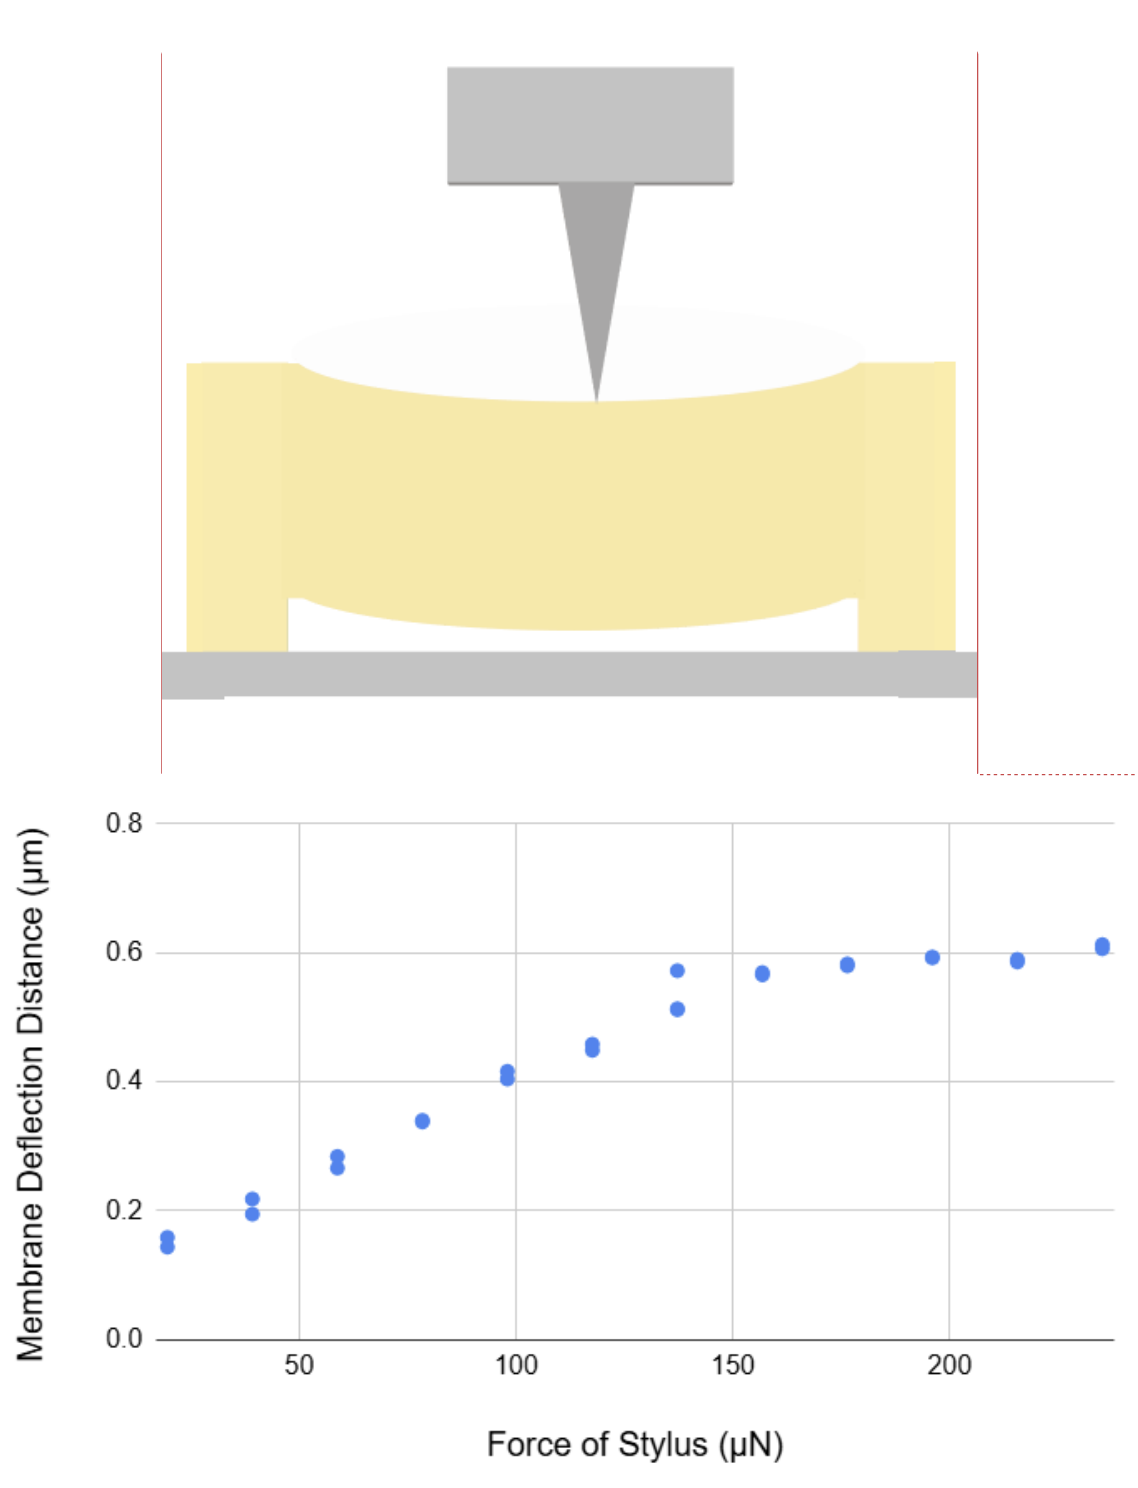
\includegraphics[width=0.7\textwidth]{figs/4-Raman/profilometer.png}
  \caption{Needle profilometer force-deflection measurements (illustrated above) performed on the suspended polymer membrane of the photonic-phononic waveguide. The inverse slope of the data (taken to be linear) is proportional to the tension of the membrane (\(m\propto T\)). Using \(m\sim\)\SI{300}{\newton\per\meter}, we estimate the tension of the membrane to be \(T\sim\)\SI{2}{\milli\newton\per\meter}, giving a very slow transverse sound speed \(v_{\rm s}\sim\)\SI{1}{\meter\per\second} via Equation~\ref{eq:Raman:TransverseSoundSpeed}.}
  \label{fig:Raman:profilometer}
\end{figure}

\begin{figure}[t]
  \centering
  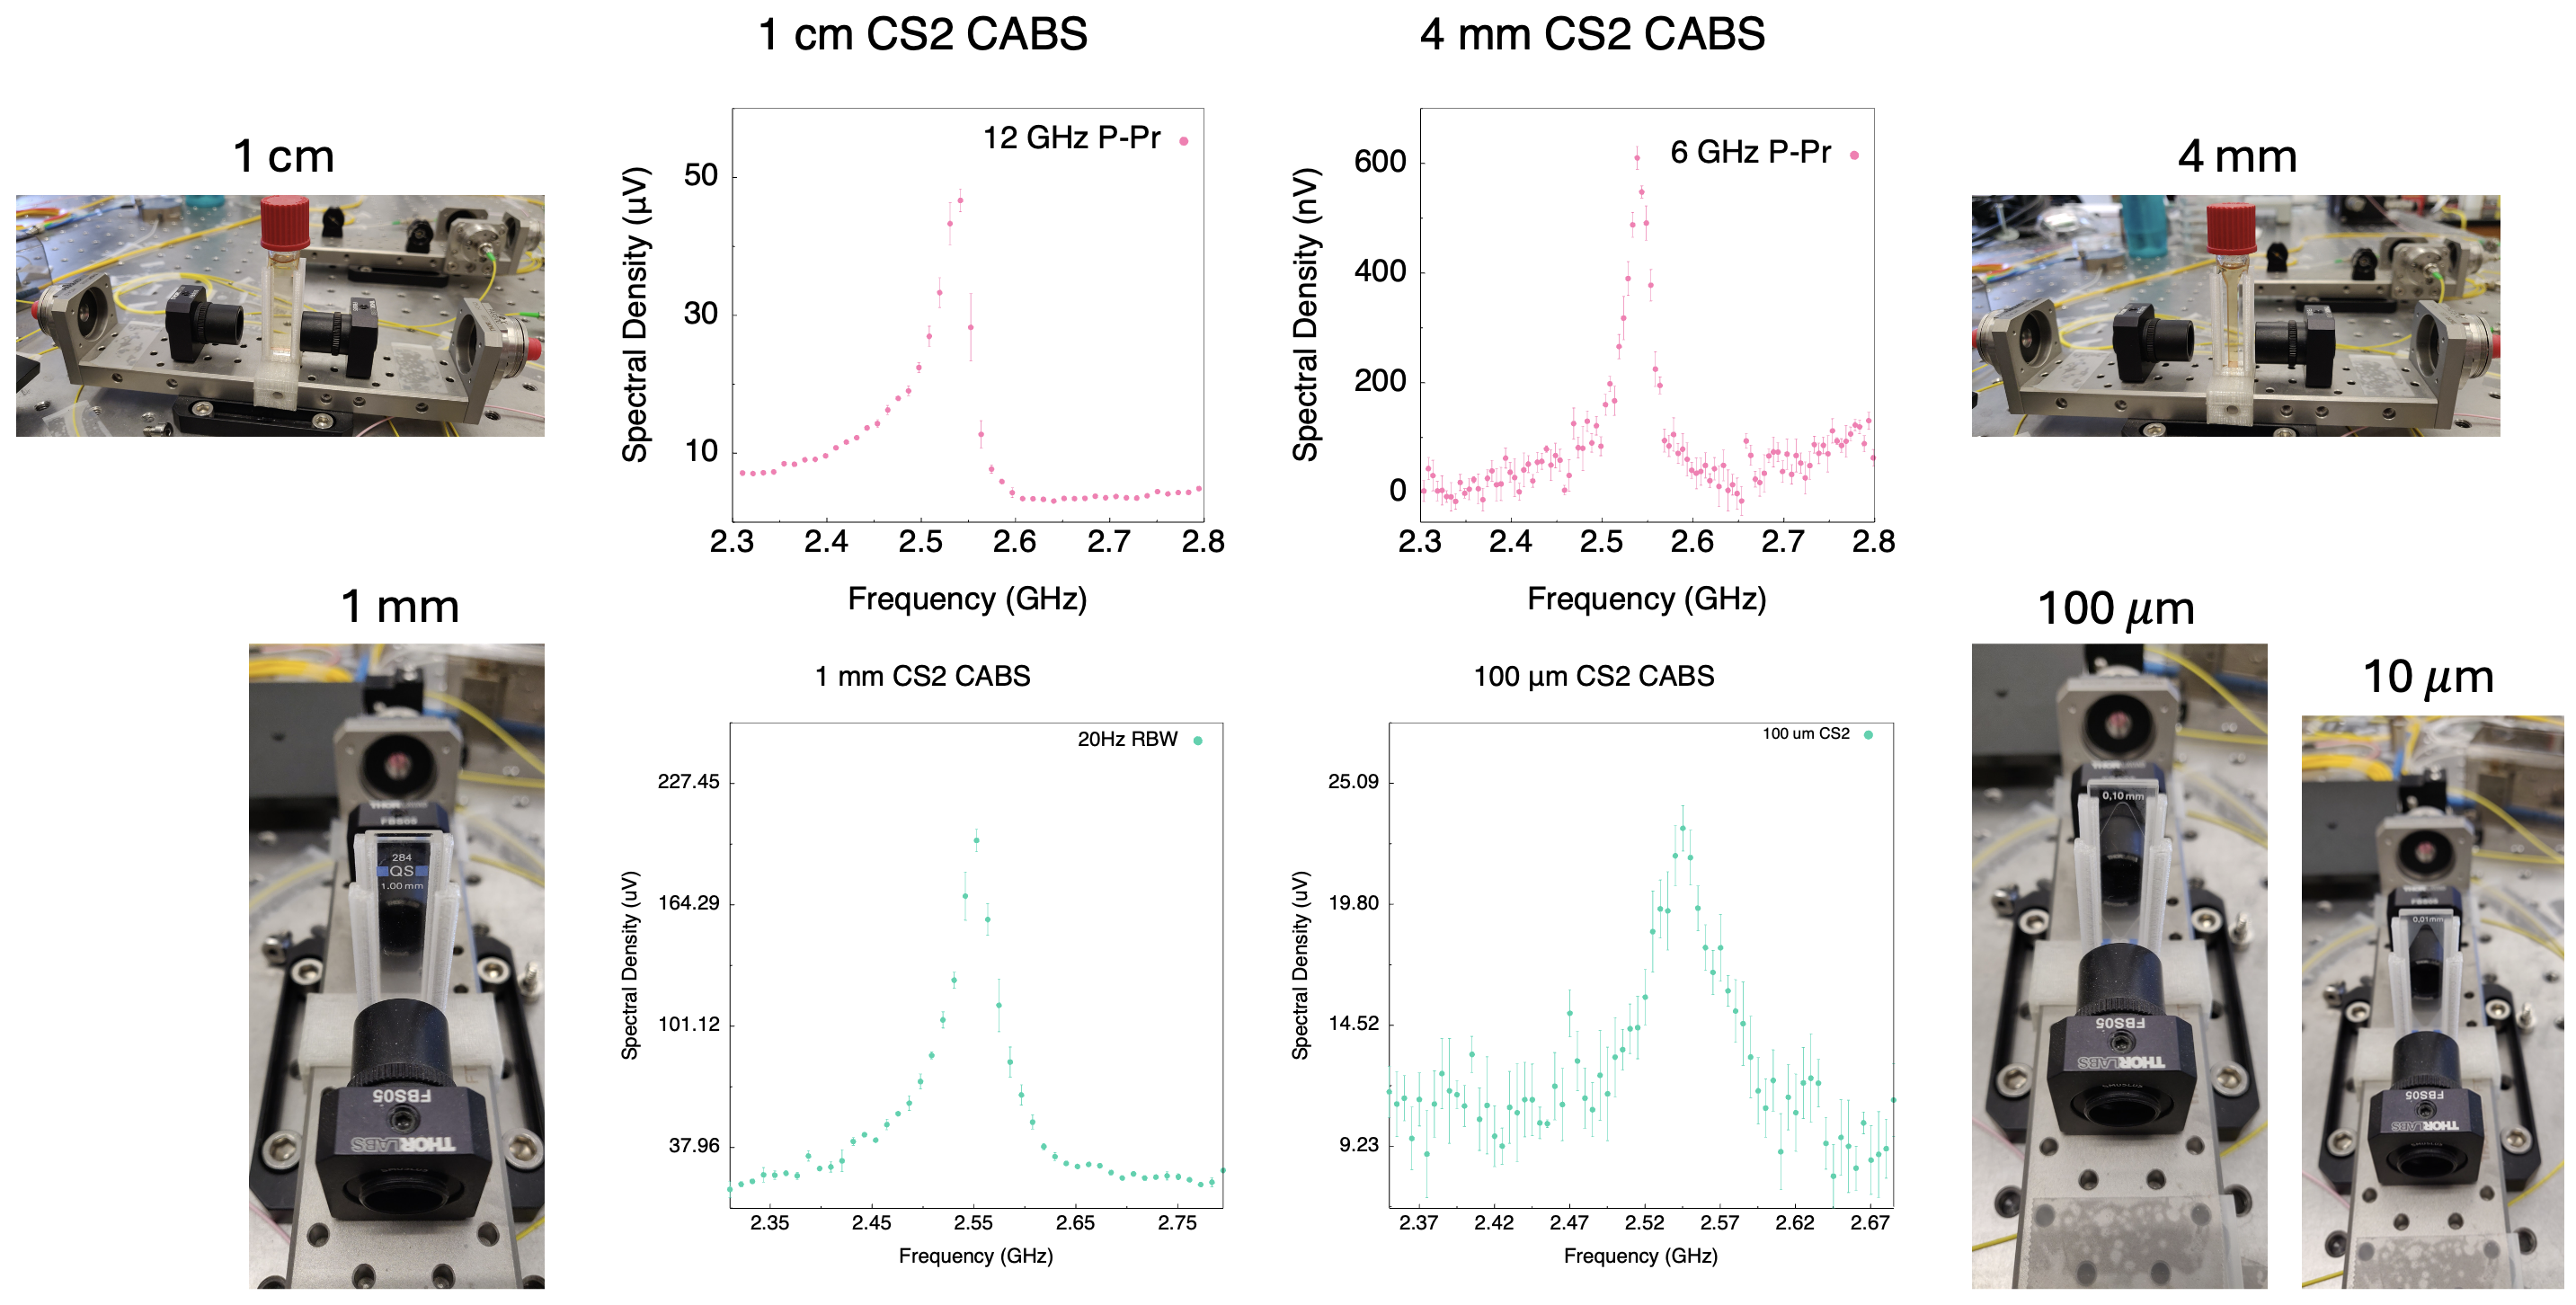
\includegraphics[width=\textwidth]{figs/4-Raman/StartBigApproachSmall.png}
  \caption{Start big, approach small.}
  \label{fig:StartBigApproachSmall}
\end{figure}

\begin{figure}[t]
  \centering
  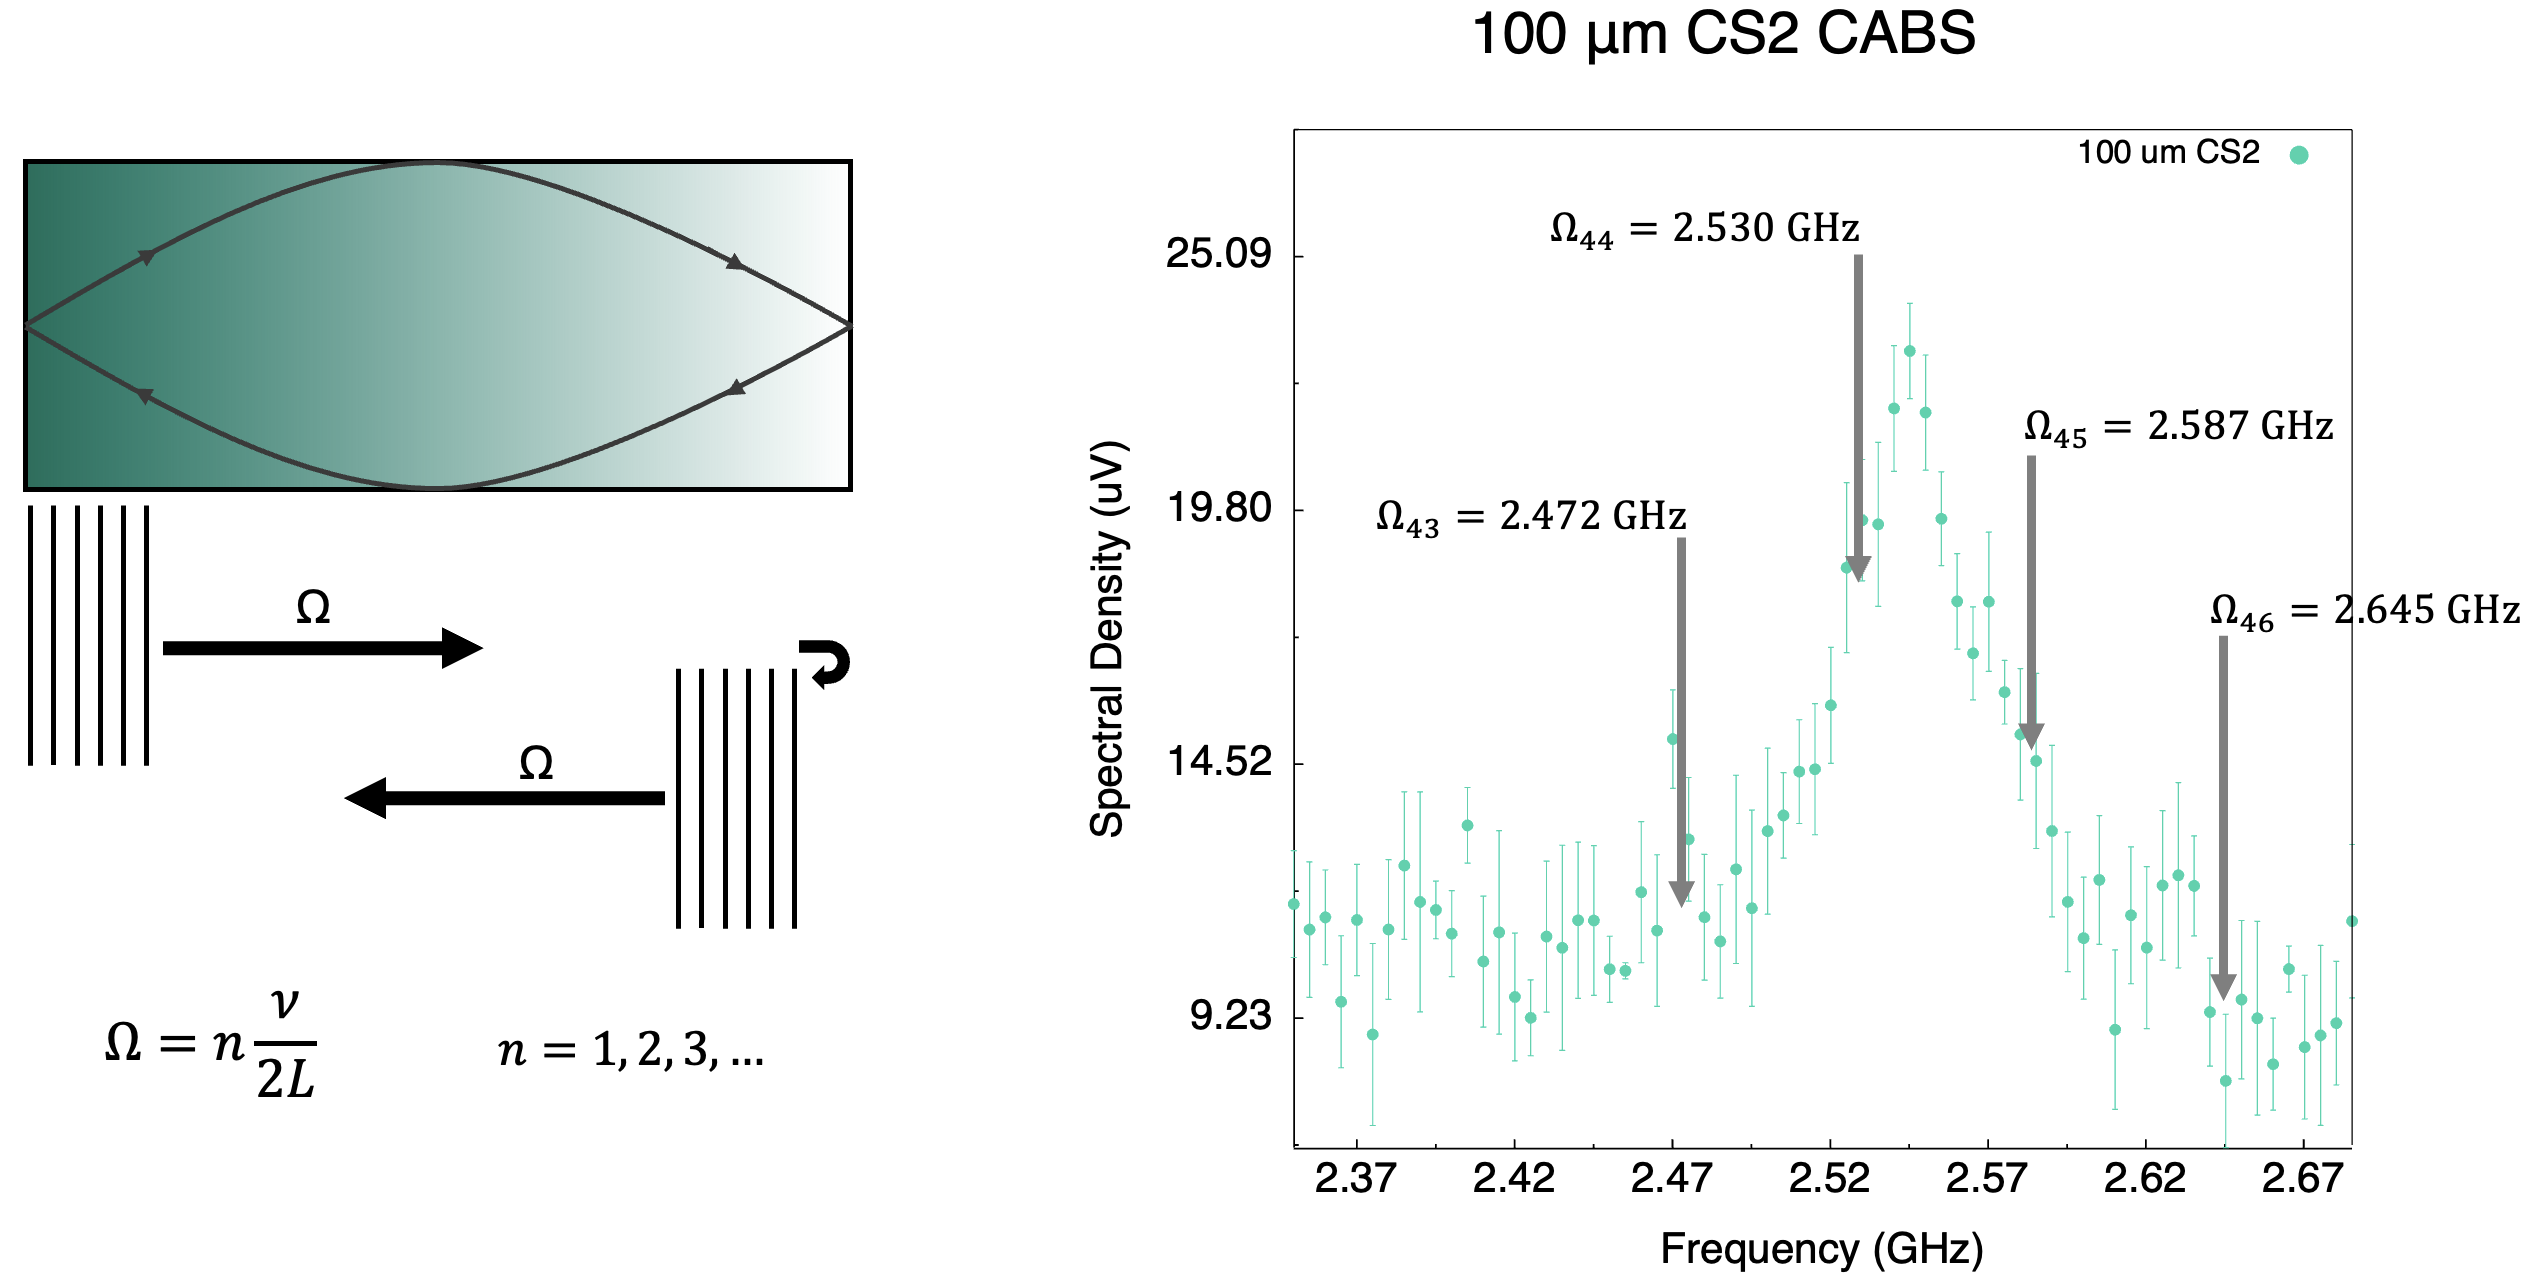
\includegraphics[width=\textwidth]{figs/4-Raman/HowWouldRamanModesAppear.png}
  \caption{How would Raman modes appear.}
  \label{fig:HowWouldRamanModesAppear}
\end{figure}

%--------------------------------------------------------------------%

\section{Discussion}
\label{sec:Raman:Discussion}

\subsection{Pathways to Brillouin-Induced Raman Modes}
\label{subsec:Raman:Pathways}

Ideal platforms by category
\begin{itemize}
  \item waveguide - long TeO2 rib, evenly spaced square holes
  \item TeO2 thin film/crystal - dissolve only small area of substrate for beam spot
  \item CS2 cell - 5um
  \item Fiber - notched, acoustic fiber Bragg grating
\end{itemize}

\subsection{Conclusion}
\label{subsec:Raman:Conclusion}

Connection to Dissertation Theme
\begin{itemize}
  \item Relate back to the broader aims of controlling phonons at room temperature, highlighting how these efforts extend exploration of optomechanical interactions.
\end{itemize}

\clearpage
\thispagestyle{empty}
\null
\newpage


%\setcounter{rownumber}{0}
\singlespacing
\chapter{Manuscript IV: Nanoscale Brillouin scattering}
\label{chap:chapterIV}
\acresetall

%  Copy this file for each main chapter, make sure to add it to main.tex

% Example author list with footnote style affiliations
%
% Christian J. Tai Udovicic\footnote{\label{spweather:nau}\ac{NAU}, \ac{DAPS}, PO Box 6010, Flagstaff, AZ 86011, USA}, Emily S. Costello\footnote{University of Hawai'i at Manoa, Honolulu, HI, USA}, Rebecca R. Ghent\footnote{Planetary Science Institute, Tucson, AZ, USA}, Christopher S. Edwards$^\mathrm{\ref{spweather:nau}}$

%  Extra copyright disclaimer to be safe
%
% \textit{This is the Accepted Manuscript version of an article accepted for publication in \ac{GRL}. Wiley Inc is not responsible for any errors or omissions in this version of the manuscript or any version derived from it. The Version of Record is available online at} \url{https://doi.org/10.1029/2020GL092198}\textit{.}

\doublespacing

%%%%%%%%%%%%%%%%%%%%%%%%%%%%%%%%%%%%%%%%%%%%%%%%%%%%%%%%%%%%%%%%%%%%
%  Chapter contents here

\section{Abstract}
\lipsum[2]


\section{Introduction}
\lipsum[2]

\begin{table}[htb]
\caption{Table caption.}
\centering
\begin{tabular}{l l c l}
\hline
& Parameter & Value & Description  \\
\hline
\multirow{5}{6em}{Lookup Variables}
 & lat  & -85$\degree$--85$\degree$ & Latitude (35 bins in 5$\degree$ increments)  \\
 & ALBEDO  & 0.05--0.225 & Bolometric albedo (6 bins in 0.035 increments)  \\
 & SLOPE  & 0$\degree$--90$\degree$ & Surface slope (19 bins in 5$\degree$ increments)   \\
 & SLOAZI  & 0$\degree$--360$\degree$ & Surface azimuth (19 bins in 20$\degree$ increments)   \\
 & DELLS  & 4$\degree$ & $L_s$ step size (90 bins spanning 0$\degree$--360$\degree$) \\
\hline
\multirow{8}{6em}{Thermal Parameters}
 & EMISS  & 0.96 & Emissivity  \\
 & thick  & 0.05 & Upper layer thickness [m] \\
 & DENSITY  & 1100 & Upper layer density [kg/m$^3$]  \\
 & DENS2  & 1800 & Lower layer density [kg/m$^3$]  \\
 & lbound  & 18 & Interior heat flow [mW/m$^2$]   \\
 & \multirow{3}{*}{PhotoFunc}  & \multirow{3}{*}{0.045/albedo} & \multirow{3}{20em}{Photometric function (Keihm-style)} \\
 & & & \\
 & & & \\
\hline
\multirow{12}{6em}{Temperature-dependent parameters}
 & SphUp0/SphLo0  & 602.88098583 & \multirow{4}{20em}{Specific heat capacity expressed as 4th-order polynomial ($\rm c0 + c1 \cdot T + c2 \cdot T^2 + c3 \cdot T^3$)} \\
 & SphUp1/SphLo1  & 235.98988249 &  \\
 & SphUp2/SphLo2  & -29.59742178 &  \\
 & SphUp3/SphLo3  & -3.78707193  & \\
 \\
 & ConUp0  & 0.00133644 &  \multirow{4}{20em}{Upper layer conductivity expressed as 4th-order polynomial ($\rm c0 + c1 \cdot T + c2 \cdot T^2 + c3 \cdot T^3$)} \\
 & ConUp1  & 0.00073150 &  \\
 & ConUp2  & 0.00033250 &  \\
 & ConUp3  & 0.00005038 &  \\
 \\
 & ConLo0  & 0.00634807 &  \multirow{4}{20em}{Lower layer conductivity expressed as 4th-order polynomial ($\rm c0 + c1 \cdot T + c2 \cdot T^2 + c3 \cdot T^3$)} \\
 & ConLo1  & 0.00347464 &  \\
 & ConLo2  & 0.00157938 &  \\
 & ConLo3  & 0.00023930 &  \\
\hline
\multirow{8}{6em}{Model Setup Parameters}
 & body  & Moon & Target body  \\
 & k\_style  & Moon & Conductivity style (Moon for airless bodies)  \\
 & LKofT  & T & Temperature-dependent conductivity  \\
 & FLAY  & 0.01 & First layer thickness [m]  \\
 & RLAY  & 1.3 & Layer thickness multiplier    \\
 & N1  & 26 & Number of layers  \\
 & N24  & 288 & Timesteps per day (5 min steps)  \\
 & DJUL  & 0 & Start date  \\
\hline
\end{tabular}
\label{stab:parametersIV}
\end{table}

\lipsum[2]


%%%%%%%%%%%%%%%%%%%% CONCLUSION %%%%%%%%%%%%%%%%%%%%%%%%%%%%%%%%%%%%%%%%%%

\chapter{Conclusion}
\label{ch:Conclusion}
\acresetall

Throughout this dissertation, we have explored how Brillouin-based optomechanics can be harnessed for both practical device applications and fundamental studies of light–matter interactions. Specifically, we demonstrated that traveling-wave phonons in an extended medium, such as a liquid-core optical fiber, can be cooled significantly through the anti-Stokes Brillouin scattering process. This result marks an important step in transitioning from the established model of discrete cavity modes toward the more general case of continuous-waveguide phonons, showing that key regimes of laser cooling can be accessed without relying on highly engineered photonic microstructures.

In tandem, this dissertation introduced the concept of a coherently stimulated Brillouin spectrometer (CoBS), which relaxes traditional phase-matching constraints and dramatically increases measurement sensitivity for short-length or low-gain samples. By incorporating a four-wave mixing scheme—pump, probe, driven Stokes, and backscattered signal—the spectrometer opens new avenues for measuring the mechanical modes of thin films, microscale liquid volumes, and emerging photonic–phononic waveguides. This flexibility is crucial for advancing applications ranging from precision material characterization to integrated acousto-optic devices.

Beyond traveling-wave phonons, we also proposed how Brillouin-induced Raman-like modes might be generated and observed at room temperature, potentially bridging the gap between conventional Raman spectroscopy and Brillouin acoustics. Although direct experimental realizations of these room temperature hybrid modes remain unobserved, the theoretical groundwork and device prototypes described here highlight the promise of such approaches for both fundamental and applied research. Ultimately, these efforts underscore the rich variety of phononic phenomena accessible when one leverages strong acousto-optic interactions in engineered media.

Looking ahead, an important direction will be to pursue net phonon cooling in waveguides by minimizing or routing away the unwanted Stokes contributions. Achieving such deep cooling could open pathways to ground-state phonon occupancy, enabling quantum acoustic memory and photon–phonon entanglement protocols. In tandem, refining the CoBS method to push detection limits and spatial resolution even further may help unlock additional device architectures across the fields of quantum information, ultralow-noise photonics, and advanced sensing. In this way, the work presented herein lays the foundation for continued innovation at the intersection of photonics, phononics, and materials science.

\clearpage
\thispagestyle{empty}
\null
\newpage


%%%%%%%%%%%%%%%%%%% APPENDICES %%%%%%%%%%%%%%%%%%%%%%%%%%%%%%%%%%%%%%%%%%%

\appendix
\singlespacing

\doublespacing
\chapter{Supplementary Information for Chapter~\ref{ch:Cooling}}
\label{Cooling:Appendix}
\acresetall

\section{Fabrication of \texorpdfstring{$CS_{2}$}{CS2}-Filled Liquid-Core Optical Fiber}
\label{Cooling:Appendix:sec:FabricationofCS2FilledLCOF}

Fabrication of the \ac{LCOF} followed the methods described by Kieu et al. (2012) \cite{kieu2012integrated}. The fabrication process involved several key steps for each of the two ends: splicing \ac{SMF-28} to \ac{UHNA7} fiber, preparing and angle-cleaving fibers, cutting and preparing a protective glass vial, and finally securing the assembly on a microscope slide. Figure \ref{fig:LCOF diagram} in the main text illustrates the overall schematic of the fiber fusion strategy, showing how \ac{SMF-28} and \ac{UHNA7} fibers flank the hollow core. The following sections detail each step in the splicing, assembly, and filling processes in fabricating the \ce{CS2}-filled \ac{LCOF}.

\subsection{Splicing}
\label{Cooling:Appendix:subsec:Splicing}

Before integrating the hollow-core segment, a segment of Corning \ac{SMF-28} was spliced to Thorlabs \ac{UHNA7} fiber. This transition was necessary to gradually match the mode fields and reduce losses at the interface with the hollow-core region.

To begin, a short length (\SI{0.5}{\meter}) of \ac{SMF-28} was stripped, cleaved flat, and arc-spliced to 5–\SI{10}{\centi\meter} of similarly prepared \ac{UHNA7} fiber. The \ac{UHNA7} fiber was fully stripped of its coating prior to arc-splicing. This was done to prevent up-and-down bending of the fiber end in subsequent horizontal alignment with the Vytran fusion splicer. The initial splice was performed with standard parameters, but the arc was then repeated four to five times in order to produce a “tapering” effect which helped narrow the \ac{SMF-28} core (\SI{9.2}{\micro\meter} diameter) where it contacted the smaller \ac{UHNA7} core (\SI{2.4}{\micro\meter} diameter), improving coupling efficiency. Prior to and following the splice, optical transmission measurements were taken to assess the splice quality and ensure maximum transmission was preserved.

After the preliminary \ac{SMF-28}–\ac{UHNA7} splice, the \ac{UHNA7} fiber needed to be angle-cleaved to ensure a gap remained for \ce{CS2} to be able to enter the hollow-core fiber after fusion-splicing the two fiber segments. An angle-cleaver with an adjustable torque and tension mechanism was used for this process. The angle-cleaved \ac{SMF-28}-\ac{UHNA7} segment was then loaded into the Vytran fusion splicing system:

\begin{enumerate}
	\item Equipment Setup: The Vytran fusion splicing station and its vacuum pump were turned on, and the system’s dedicated software interface was opened. Approximately two minutes was allowed for the vacuum level to stabilize.
	\item Fiber Positioning: The left fiber clamp block was pivoted fully to the left, and the \ac{UHNA7} fiber was placed so that its freshly cleaved tip was centered over the reference circle at the splice head.
	\item Alignment: While the vacuum held the fiber in place, the system’s camera view was used to rotate the fiber such that the sharpest angle of the \ac{UHNA7}’s end face was in the camera's view. A small “flag”—a piece of unstripped fiber with a small tape handle on one end—was used as needed to help the clamp grip the bare \ac{UHNA7} fiber securely.
	\item Pivot and Support: The left block was pivoted back and forth until the \ac{UHNA7} tip was near the correct horizontal position. A folded piece of support paper and two boxes of Kimtech Kimwipes on the benchtop were used to prevent the fiber from drooping and to minimize the risk of breakage during handling.
\end{enumerate}

\begin{figure}[t]
  \centering
  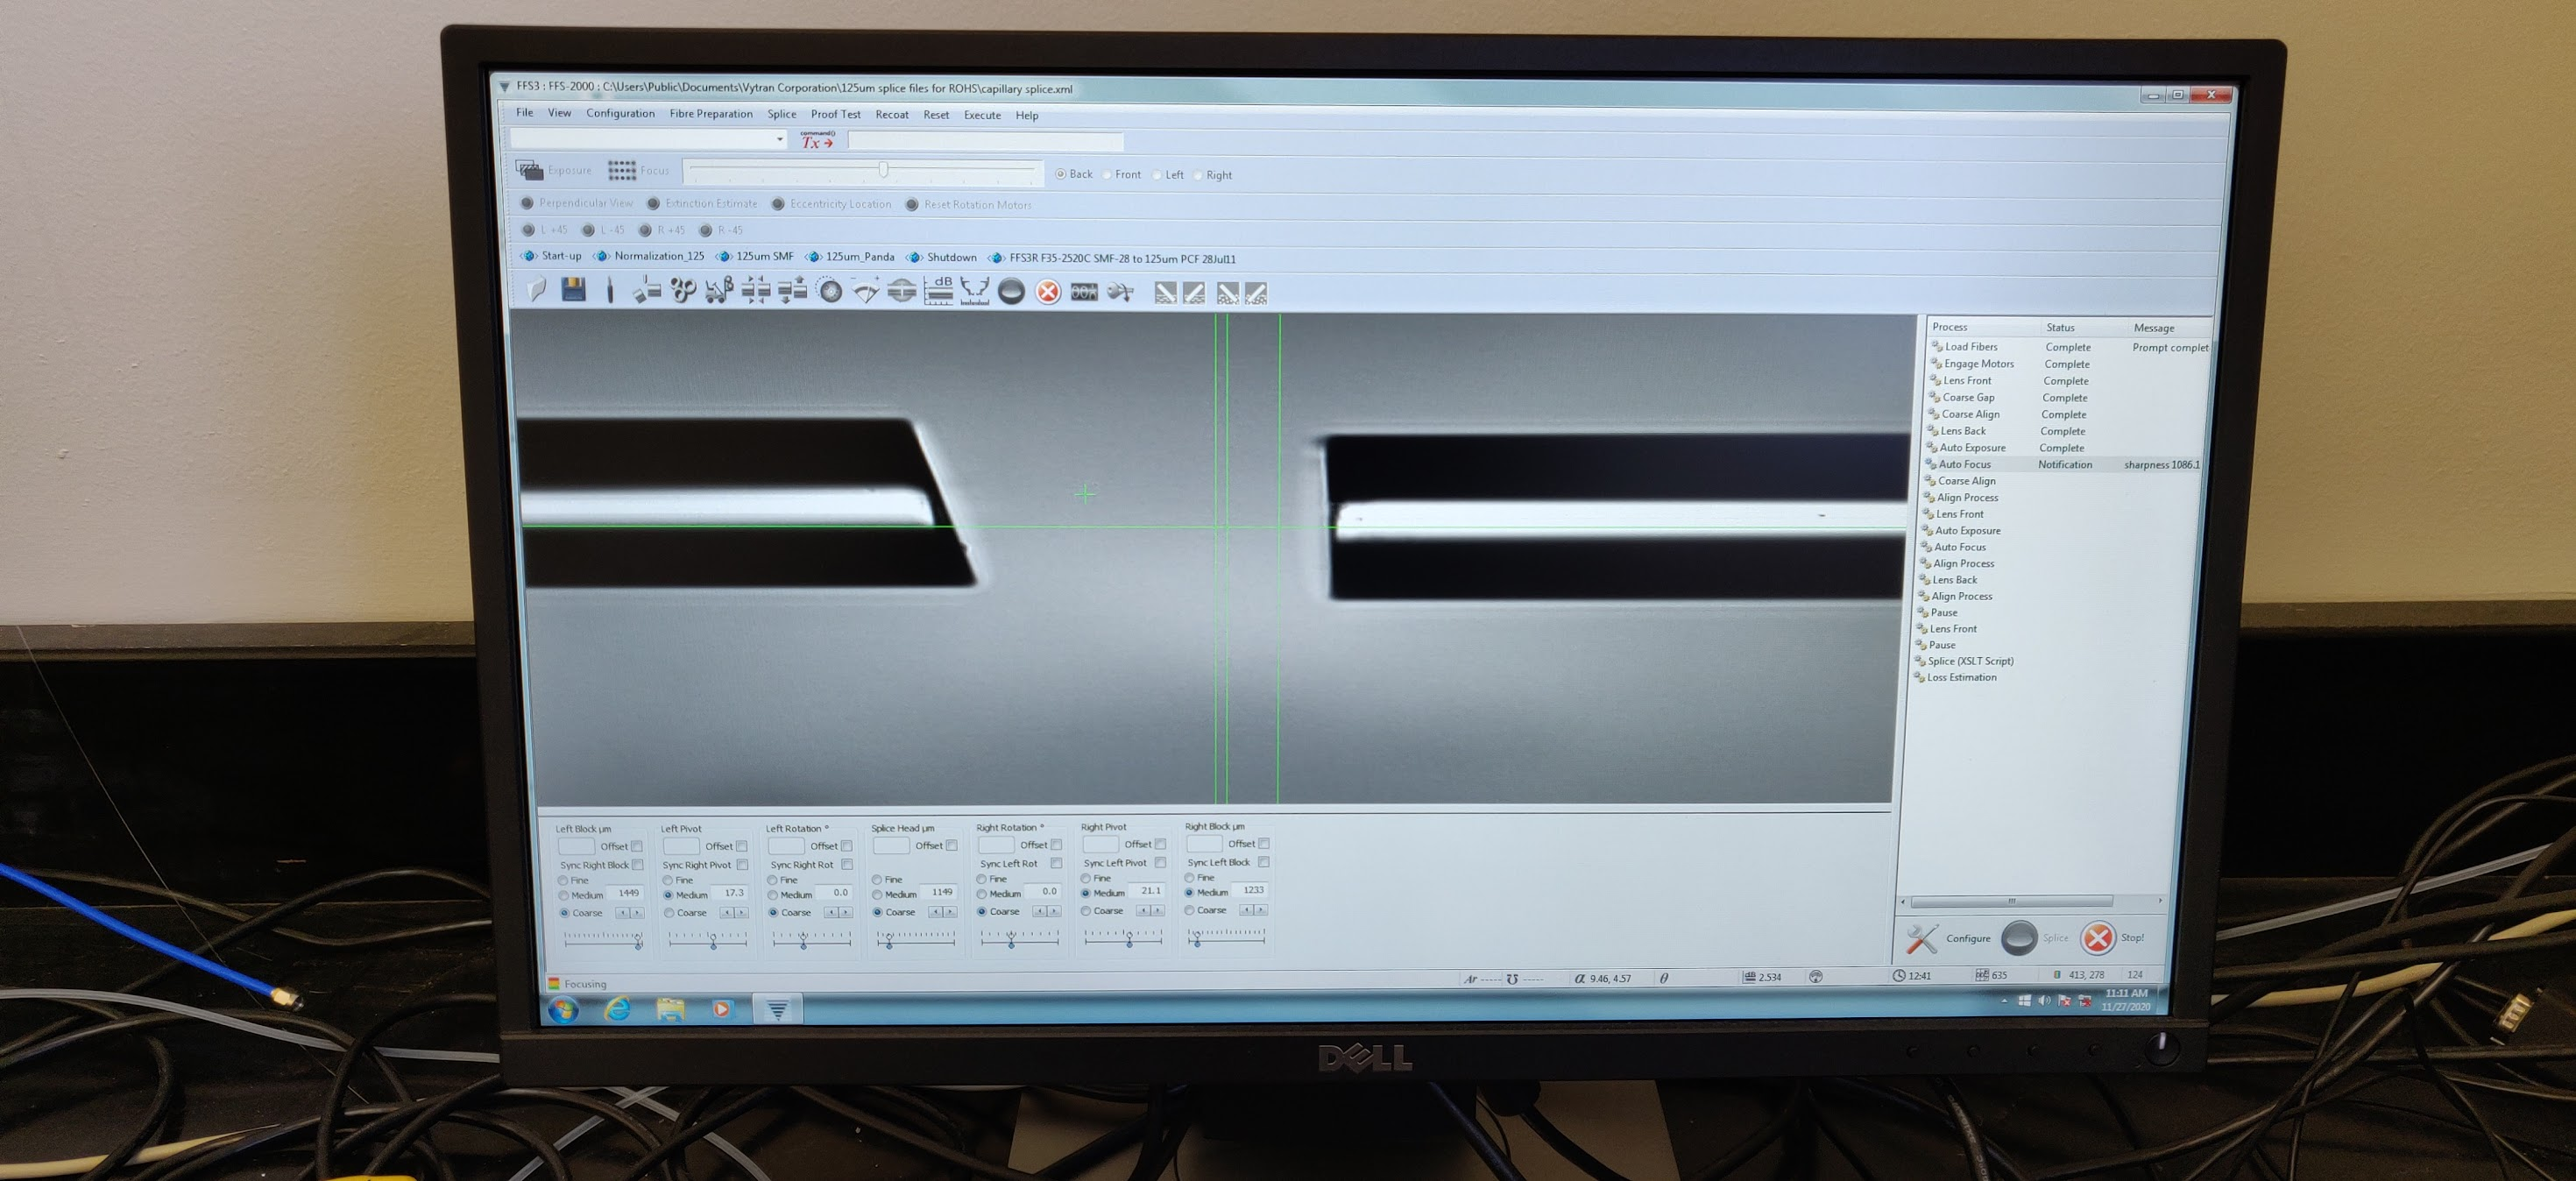
\includegraphics[width=\textwidth]{figs/2-Cooling/vytranCameraPreSplice.jpg}
  \caption{Picture of Vytran software interface camera imaging system showing a microscope view of the two fiber ends pre-splice (Section~\ref{Cooling:Appendix:subsec:Splicing}). The left angle-cleaved fiber is the \ac{UHNA7} fiber. The right flat-cleaved fiber is the hollow-core fiber. Subsequent alignment processes, first automatic then manual fine-tuning, align the fibers in xy space for optimal fusion-splicing and optical transmission once filled.}
  \label{fig:vytran camera pre splice}
\end{figure}

\begin{figure}[t!]
    \centering
    \begin{subfigure}[b]{\textwidth}
        \centering
        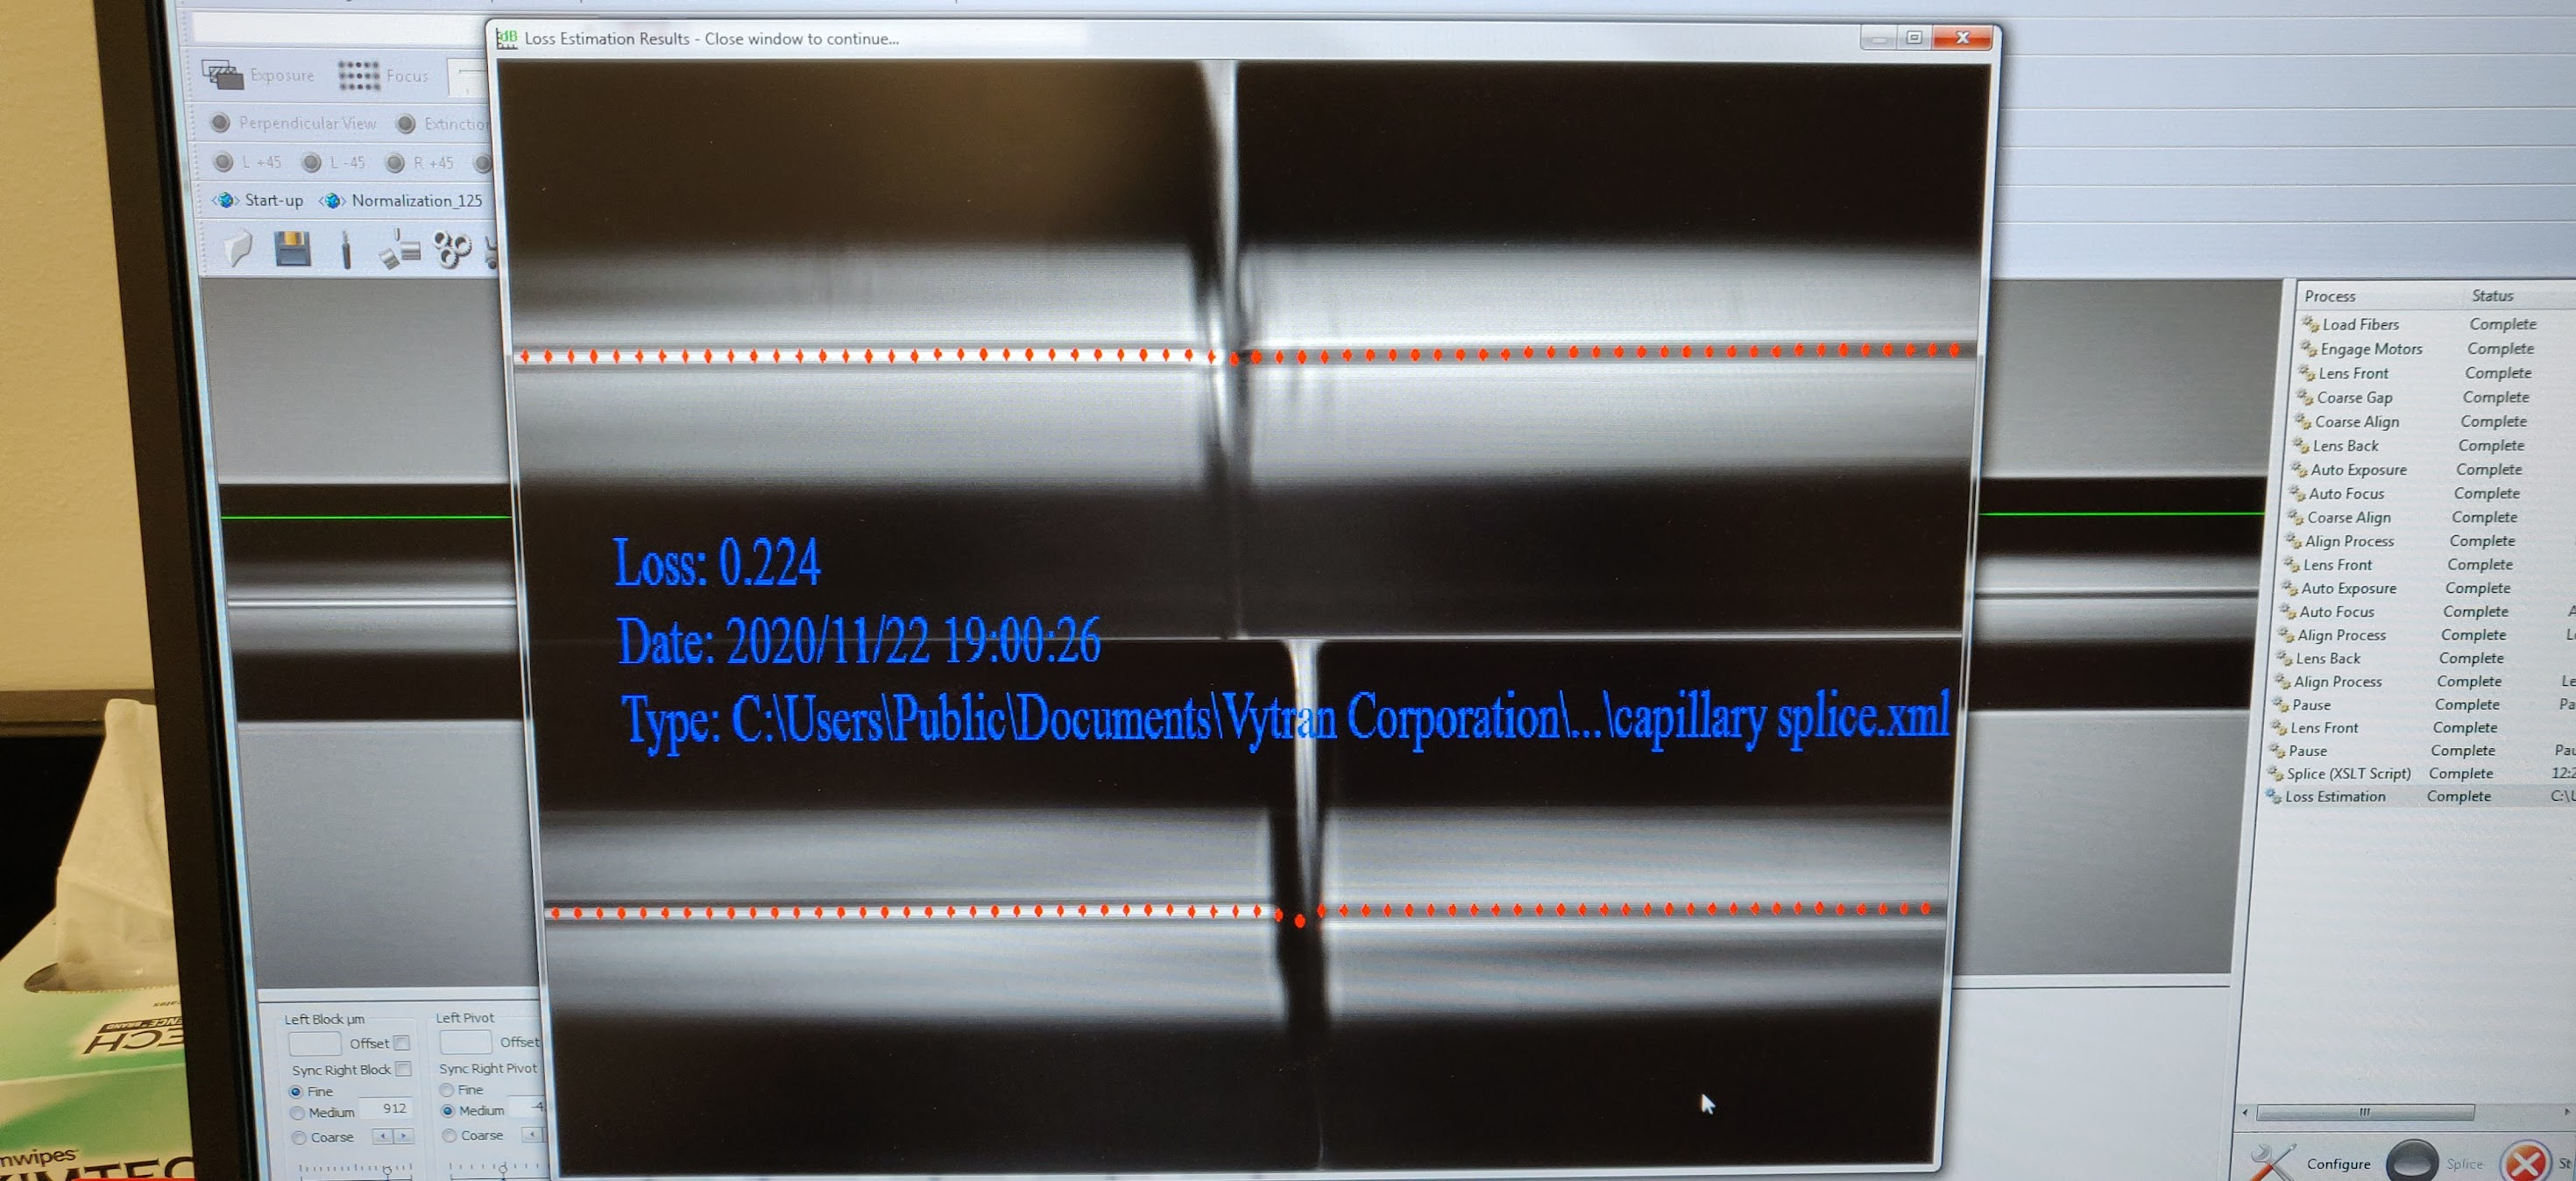
\includegraphics[width=\textwidth]{figs/2-Cooling/bigGapSplice.jpg}
        \caption{}
        \label{fig:Cooling:big gap splice}
    \end{subfigure}
    \vspace{0.5cm}
    \begin{subfigure}[b]{\textwidth}
        \centering
        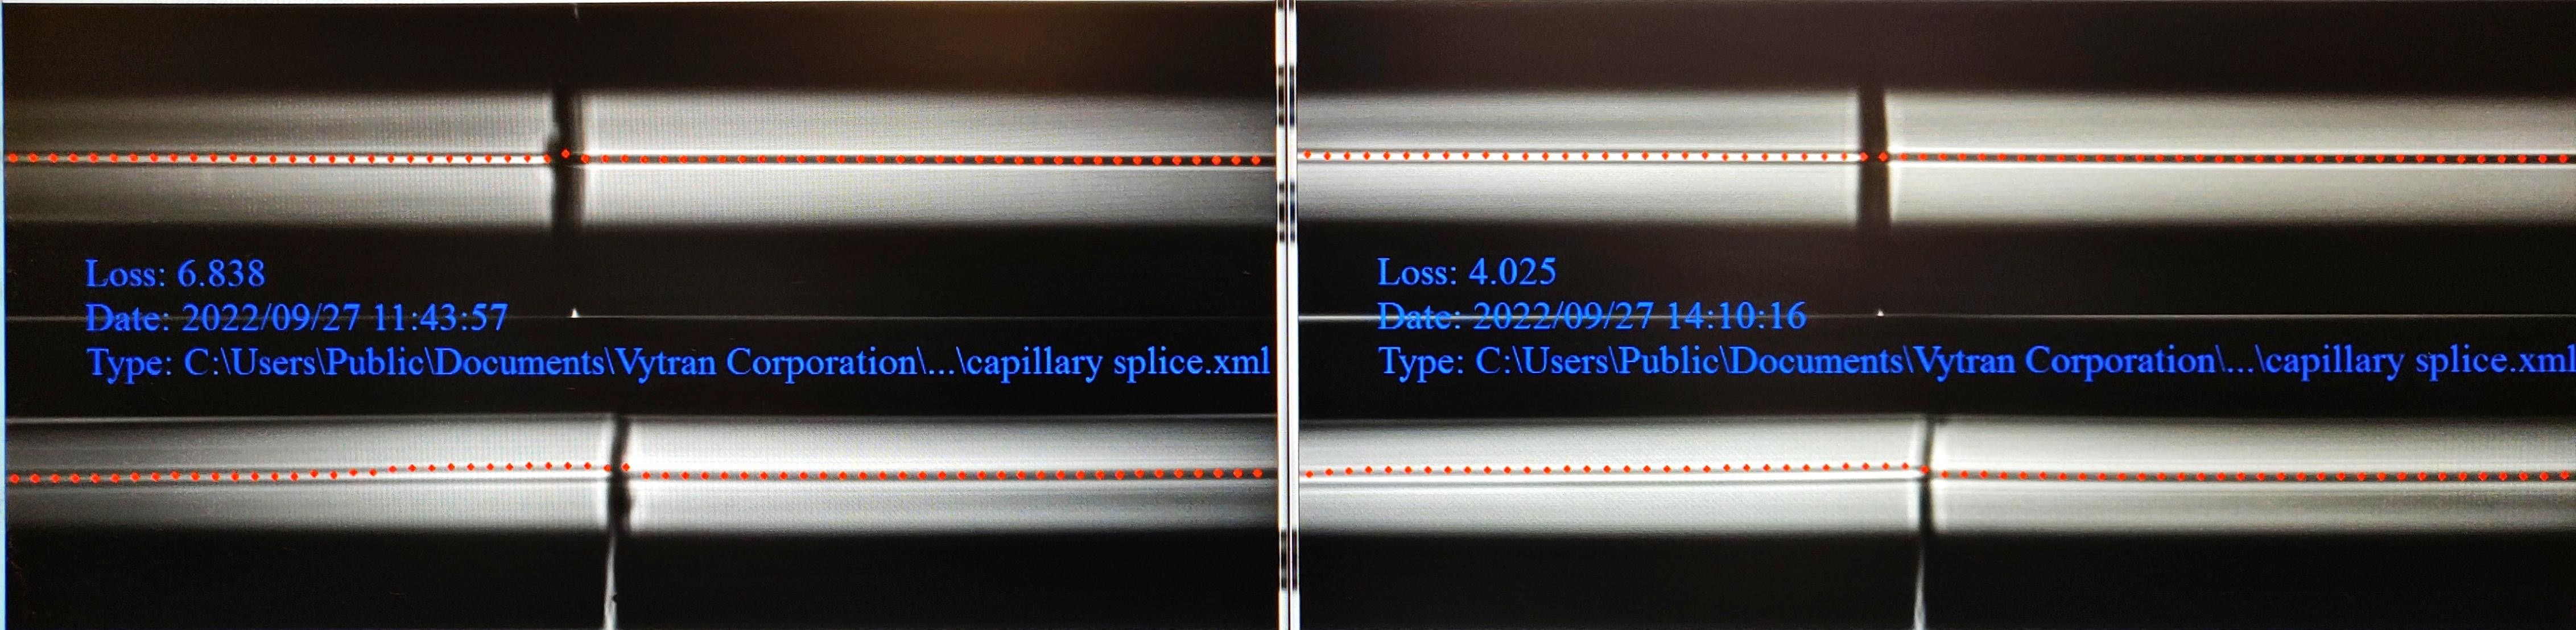
\includegraphics[width=\textwidth]{figs/2-Cooling/finalSampleVytranSplice.jpeg}
        \caption{}
        \label{fig:Cooling:final splice used for data}
    \end{subfigure}
    \caption{Example images of \ac{LCOF} splices (Section~\ref{Cooling:Appendix:subsec:Splicing}). Figure (a) shows an earlier example of a splice which featured a large visible wedge-shaped gap for liquid to enter the hollow-core fiber. While gaps of this size were sometimes successfully transferred onto a slide, further investigation showed gaps of this scale to reduce optical transmission through the splice. This fact became critical later for collecting the data for the pump-probe experiment. Figure (b) shows images of the two splices featured on the ultimate sample which was used to gather final data for publication.}
    \label{fig:Cooling:example splice images}
\end{figure}

Once the \ac{UHNA7} fiber was properly angle-cleaved, the hollow-core fiber segment was prepared for splicing:

\begin{enumerate}
	\item Stripping and Cleaving: The hollow-core fiber coating was gently dissolved in acetone and wiped away to expose the bare glass. It was then cleaved flat rather than at an angle.
	\item Positioning on the Vytran fusion splicer: The right clamp block was pivoted to its stop position, and the hollow-core fiber was placed so its end was centered over the splice head’s circle, ensuring no physical contact with the \ac{UHNA7} fiber.
	\item Flag and Alignment: As with the \ac{UHNA7}, a flag of unstripped fiber was placed above the hollow-core fiber to facilitate stable clamping. The right clamp block was slowly pivoted toward the center until the fiber tips were close but still not touching. Like before, the fiber was supported with folded paper and Kimwipe boxes to prevent bending.
\end{enumerate}

\begin{figure}[t]
  \centering
  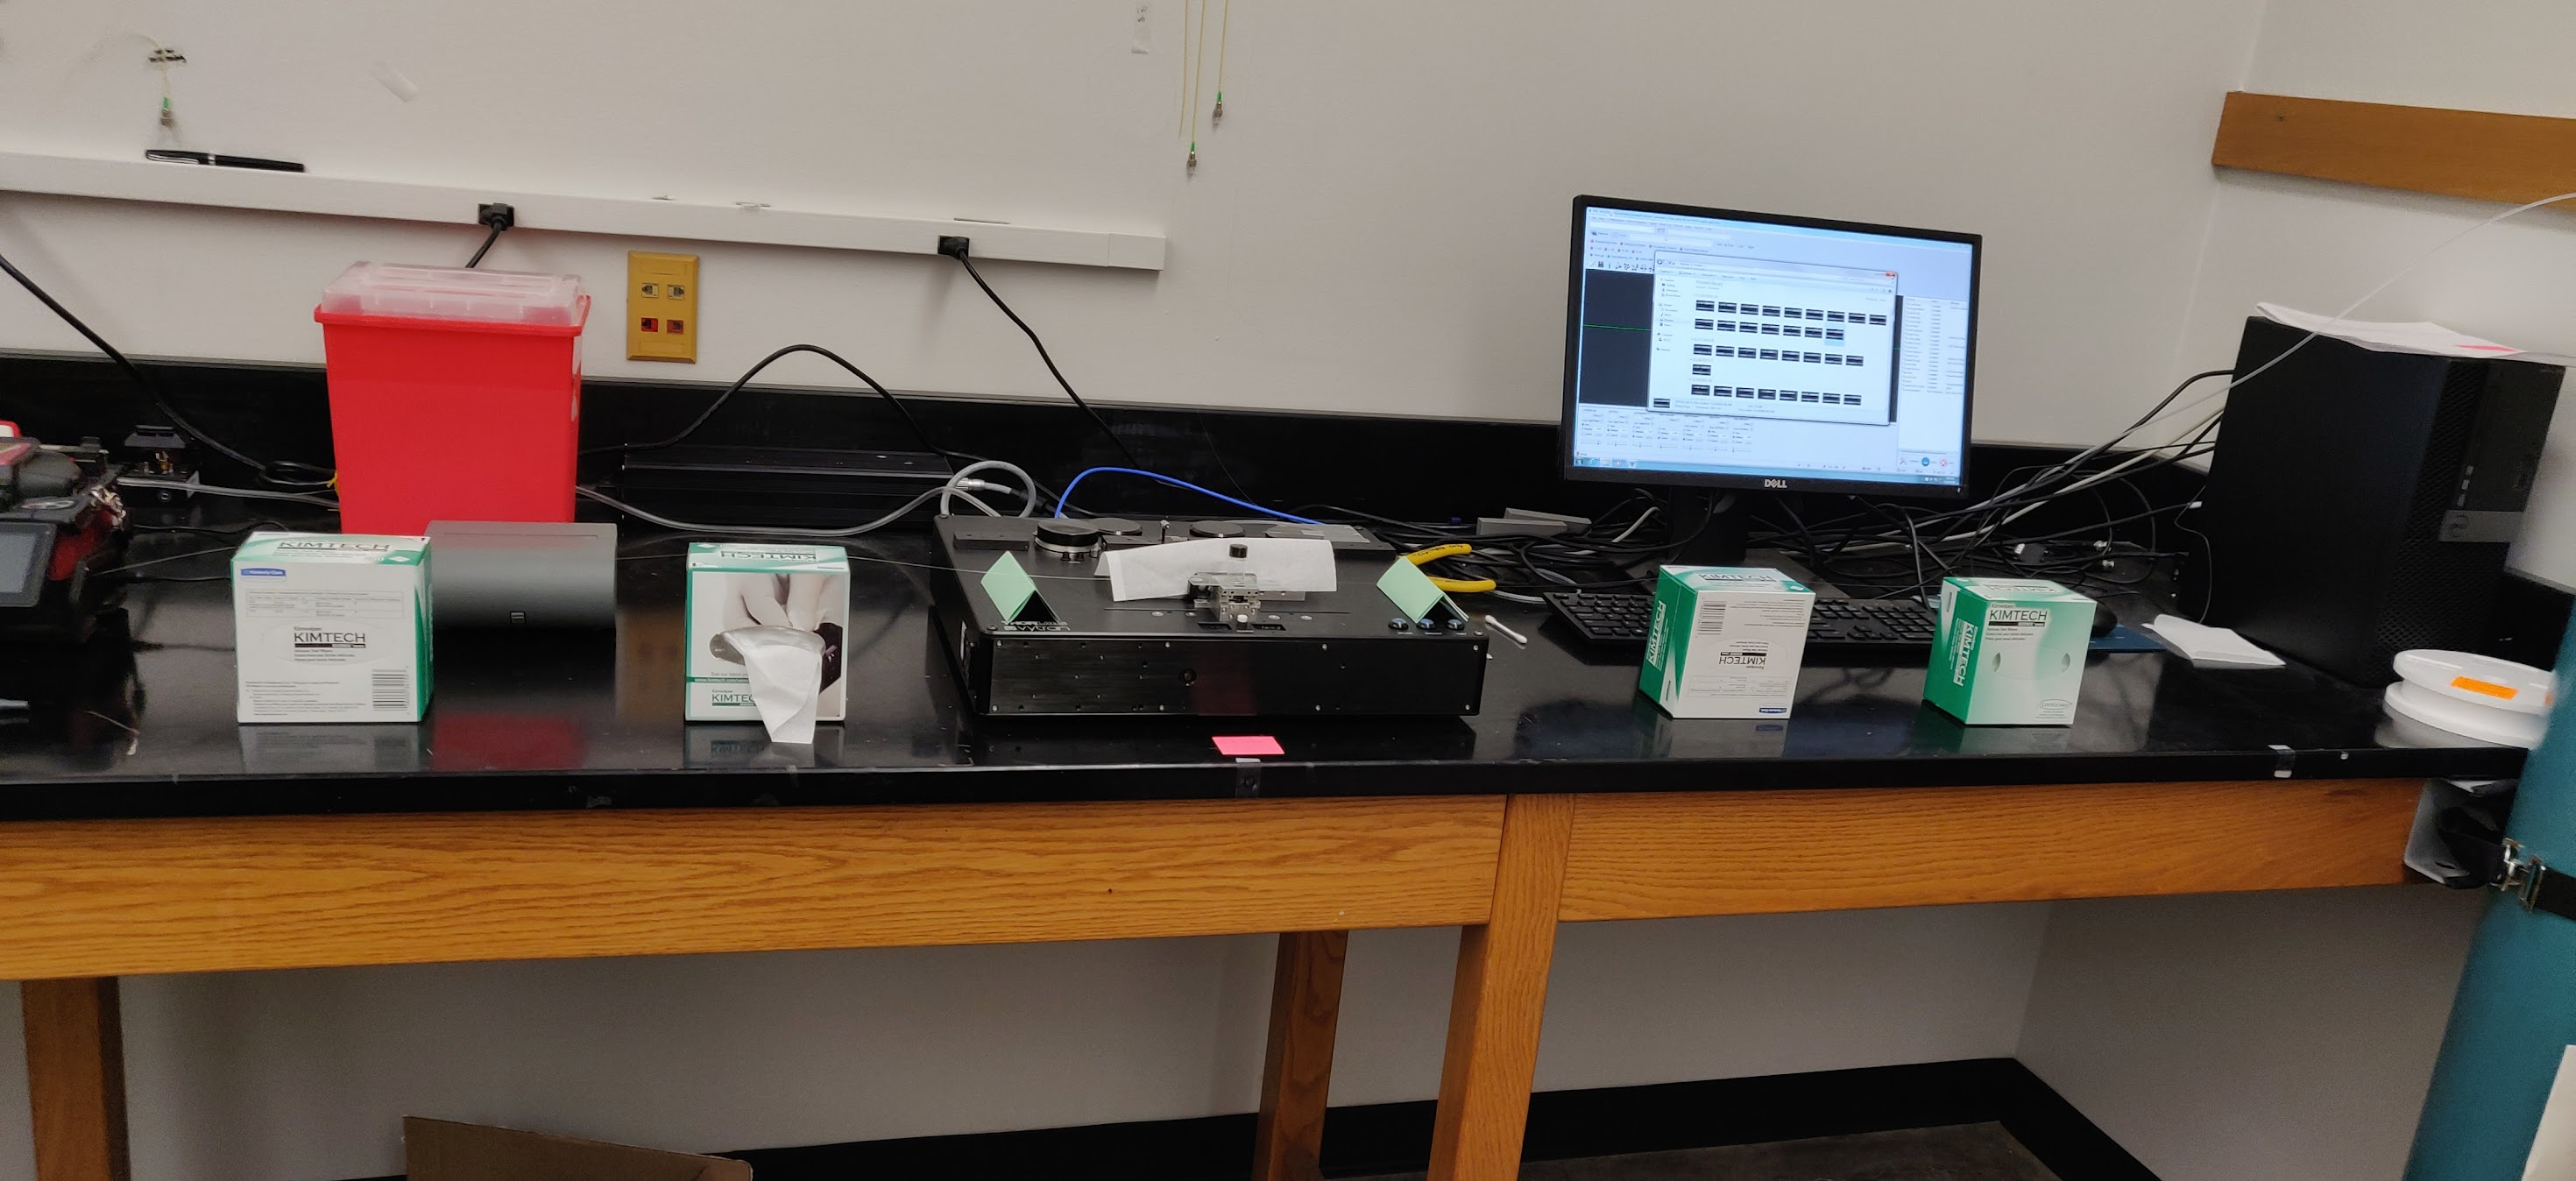
\includegraphics[width=\textwidth]{figs/2-Cooling/doubleBoxBracedSplice.jpg}
  \caption{Picture of both lengths of fiber braced by folded paper and two Kimwipe boxes on either side to prevent bending and flexing while transferring the delicate splice onto a glass slide (Section~\ref{Cooling:Appendix:subsec:Splicing}).}
  \label{fig:double box braced splice}
\end{figure}

The next step was to form the final fusion splice between the \ac{UHNA7} fiber and the hollow-core segment within the fusion splicer:

\begin{enumerate}
	\item Positioning and Auto-Alignment: With both fibers supported and extending naturally from opposite blocks, the splicer’s auto-alignment was initiated. The system brought the fibers within viewing distance so the operator could adjust vertical and horizontal positioning.
	\item Core Alignment: Using the splicer’s camera interface, the UHNA7 core was lined up with the hollow-core’s central region. Small vertical and horizontal translations ensured good overlap.
	\item Fiber Touch-Off: The left fiber (\ac{UHNA7} side) was carefully advanced until the tips touched, then retracted two clicks for optimal separation during splicing. Precise final positioning of the fiber ends ensured that a small gap remained in the hollow core to accommodate liquid infiltration during the filling process. Simultaneously, this same fiber end positioning ensured the cladding regions were fused sufficiently to preserve splice integrity under the delicate handling steps that followed.
	\item Argon Gas Flow and Fusion: An argon flow was introduced to shield the fusion region from contaminants, and the fusion filament heating was applied. Images were taken at each step to verify the splice quality. If alignment or splicing was inadequate, the fibers were separated, re-cleaved if necessary, and the procedure repeated. After confirming a good splice, the argon was turned off and the splicer was shut down.
\end{enumerate}

\begin{figure}[t]
  \centering
  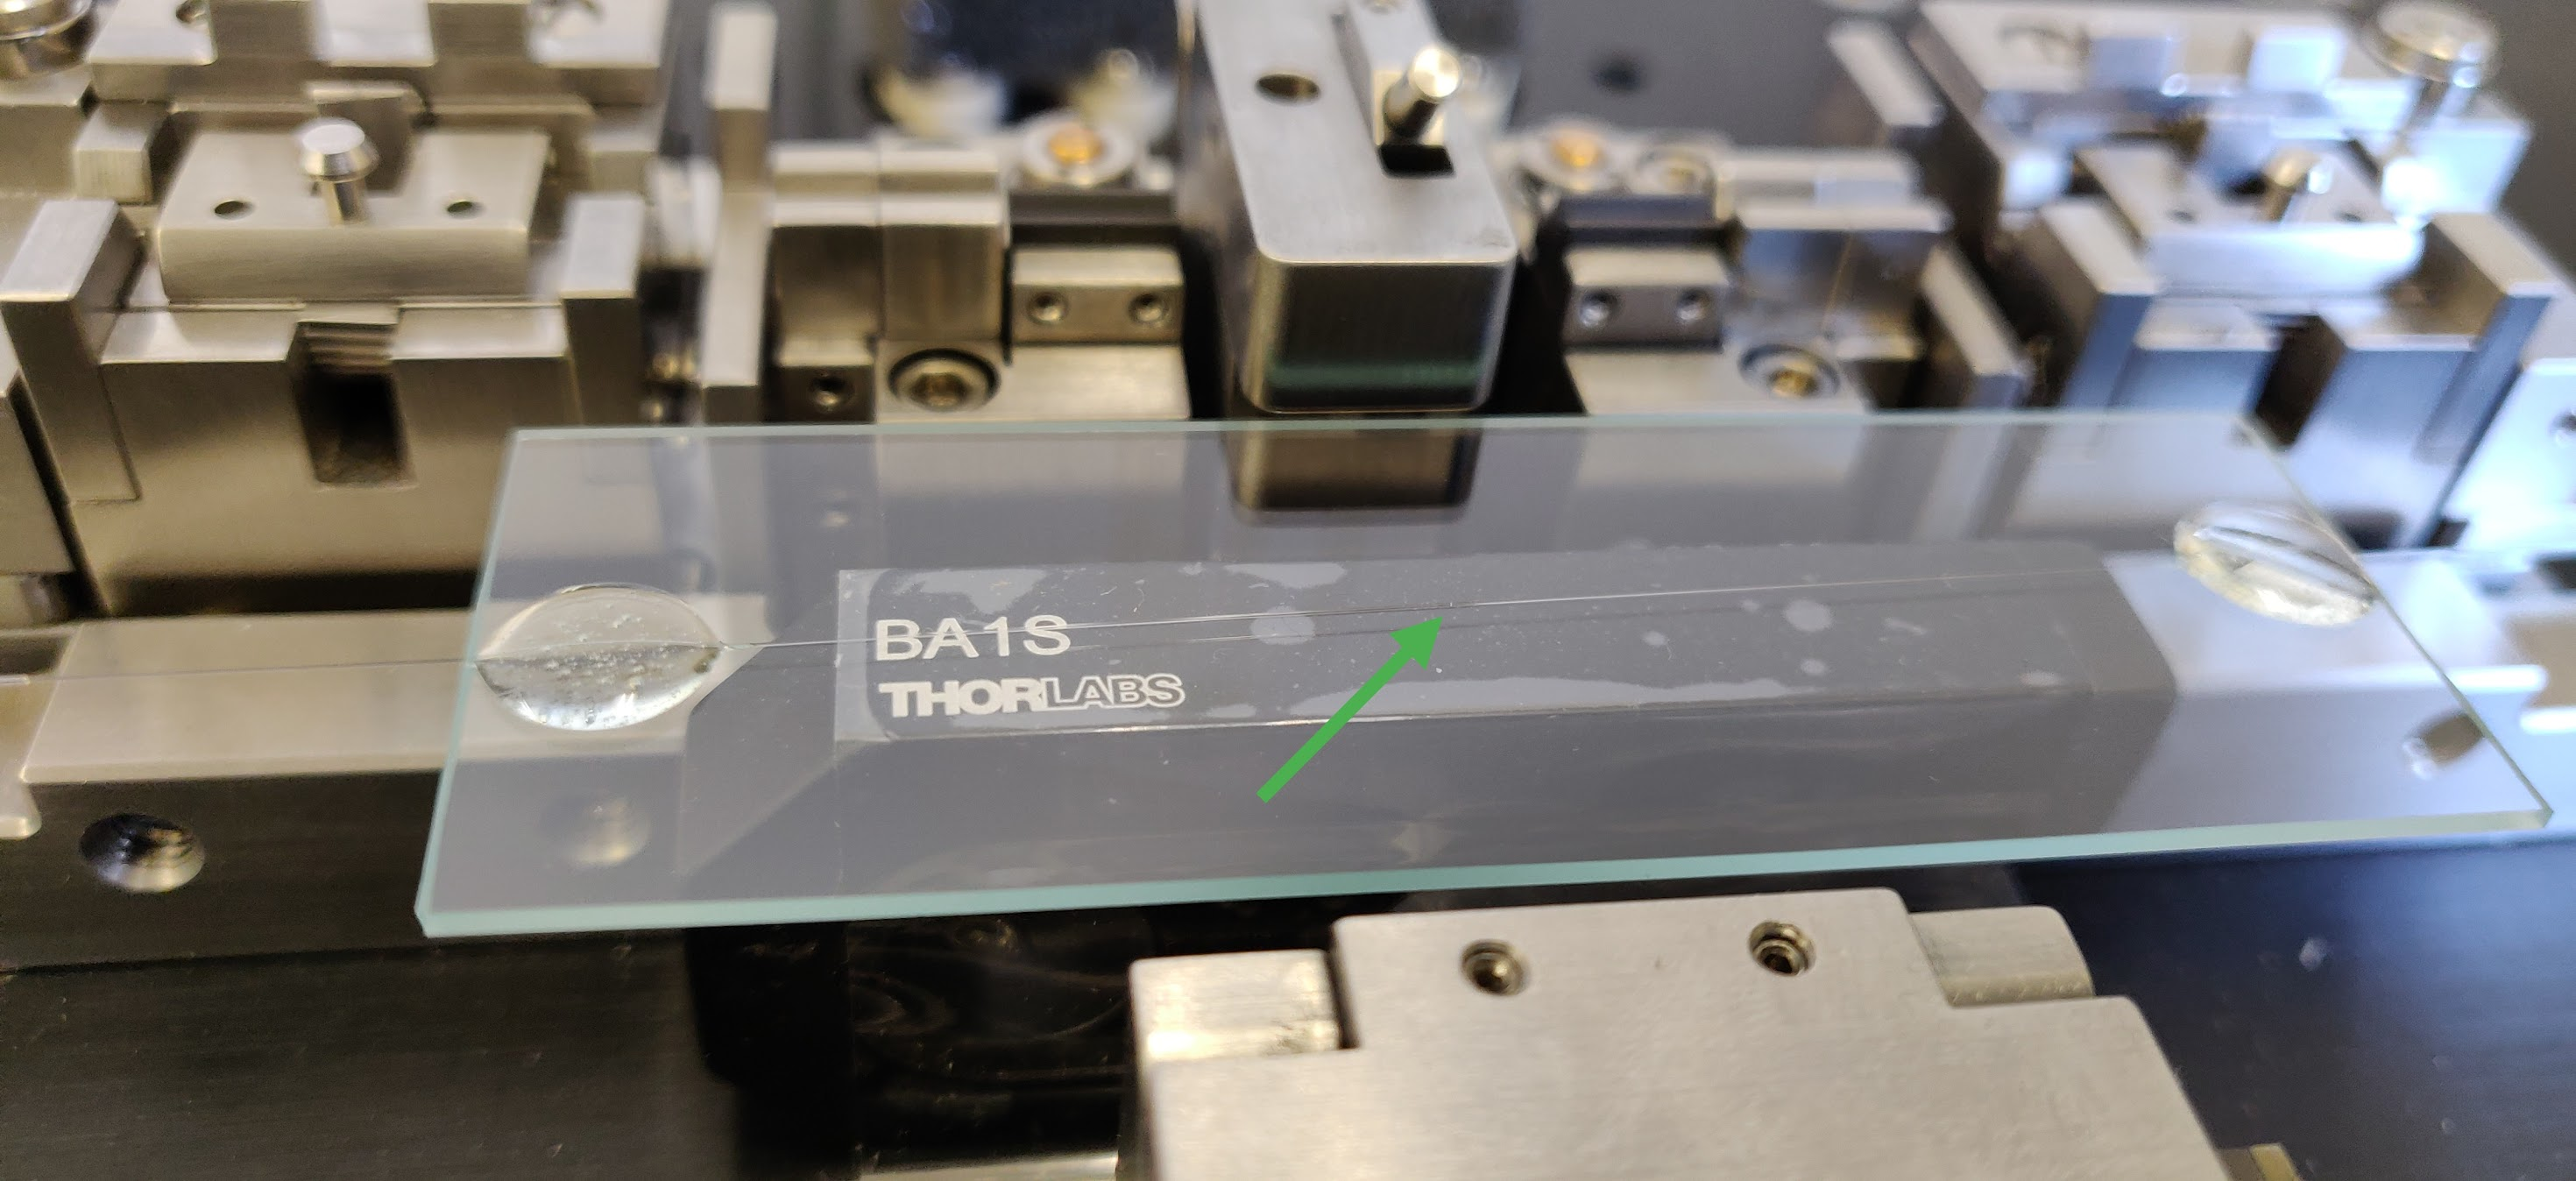
\includegraphics[width=\textwidth]{figs/2-Cooling/tackedSpliceWithArrow.jpg}
  \caption{Picture of splice successfully transferred onto a glass slide and tacked on either side with drops of epoxy (Section~\ref{Cooling:Appendix:subsec:Splicing}). An arrow points to the location of the critical splice between the angle-cleaved \ac{UHNA7} fiber and the flat-cleaved hollow-core fiber.}
  \label{fig:tacked splice with arrow}
\end{figure}

\subsection{Reservoir Assembly}
\label{Cooling:Appendix:subsec:Reservoir Assembly}

Because the final splice assembly must be encapsulated for protection, it was mounted on a clean microscope slide. The slide was scrubbed with soap and a soft toothbrush under running hot water, then thoroughly rinsed and dried with an air gun. Clean handling was crucial, so the slide was placed inside a folded Kimwipe for safekeeping until needed.

A small glass vial was used to form a protective enclosure over the splice region and allow liquid to fill the hollow core.

\begin{enumerate}
	\item Cutting the Vial: Wearing gloves and safety glasses, a new glass vial was secured carefully by hand and cut at low rotational speed on a saw. The cut removed only the bottom portion of the vial so that the main body of the vial remained relatively long.
	\item Flattening and Notching: The cut edge was smoothed and flattened with a file block, and two shallow, wide straddle-gaps were added on opposite sides of the new opening. These gaps would later accommodate the fiber on the slide.
	\item Cleaning: Finally, the vial was scrubbed with dish soap and a pipe cleaner, rinsed, dried with compressed air, and recapped until needed.
\end{enumerate}

\begin{figure}[t]
  \centering
  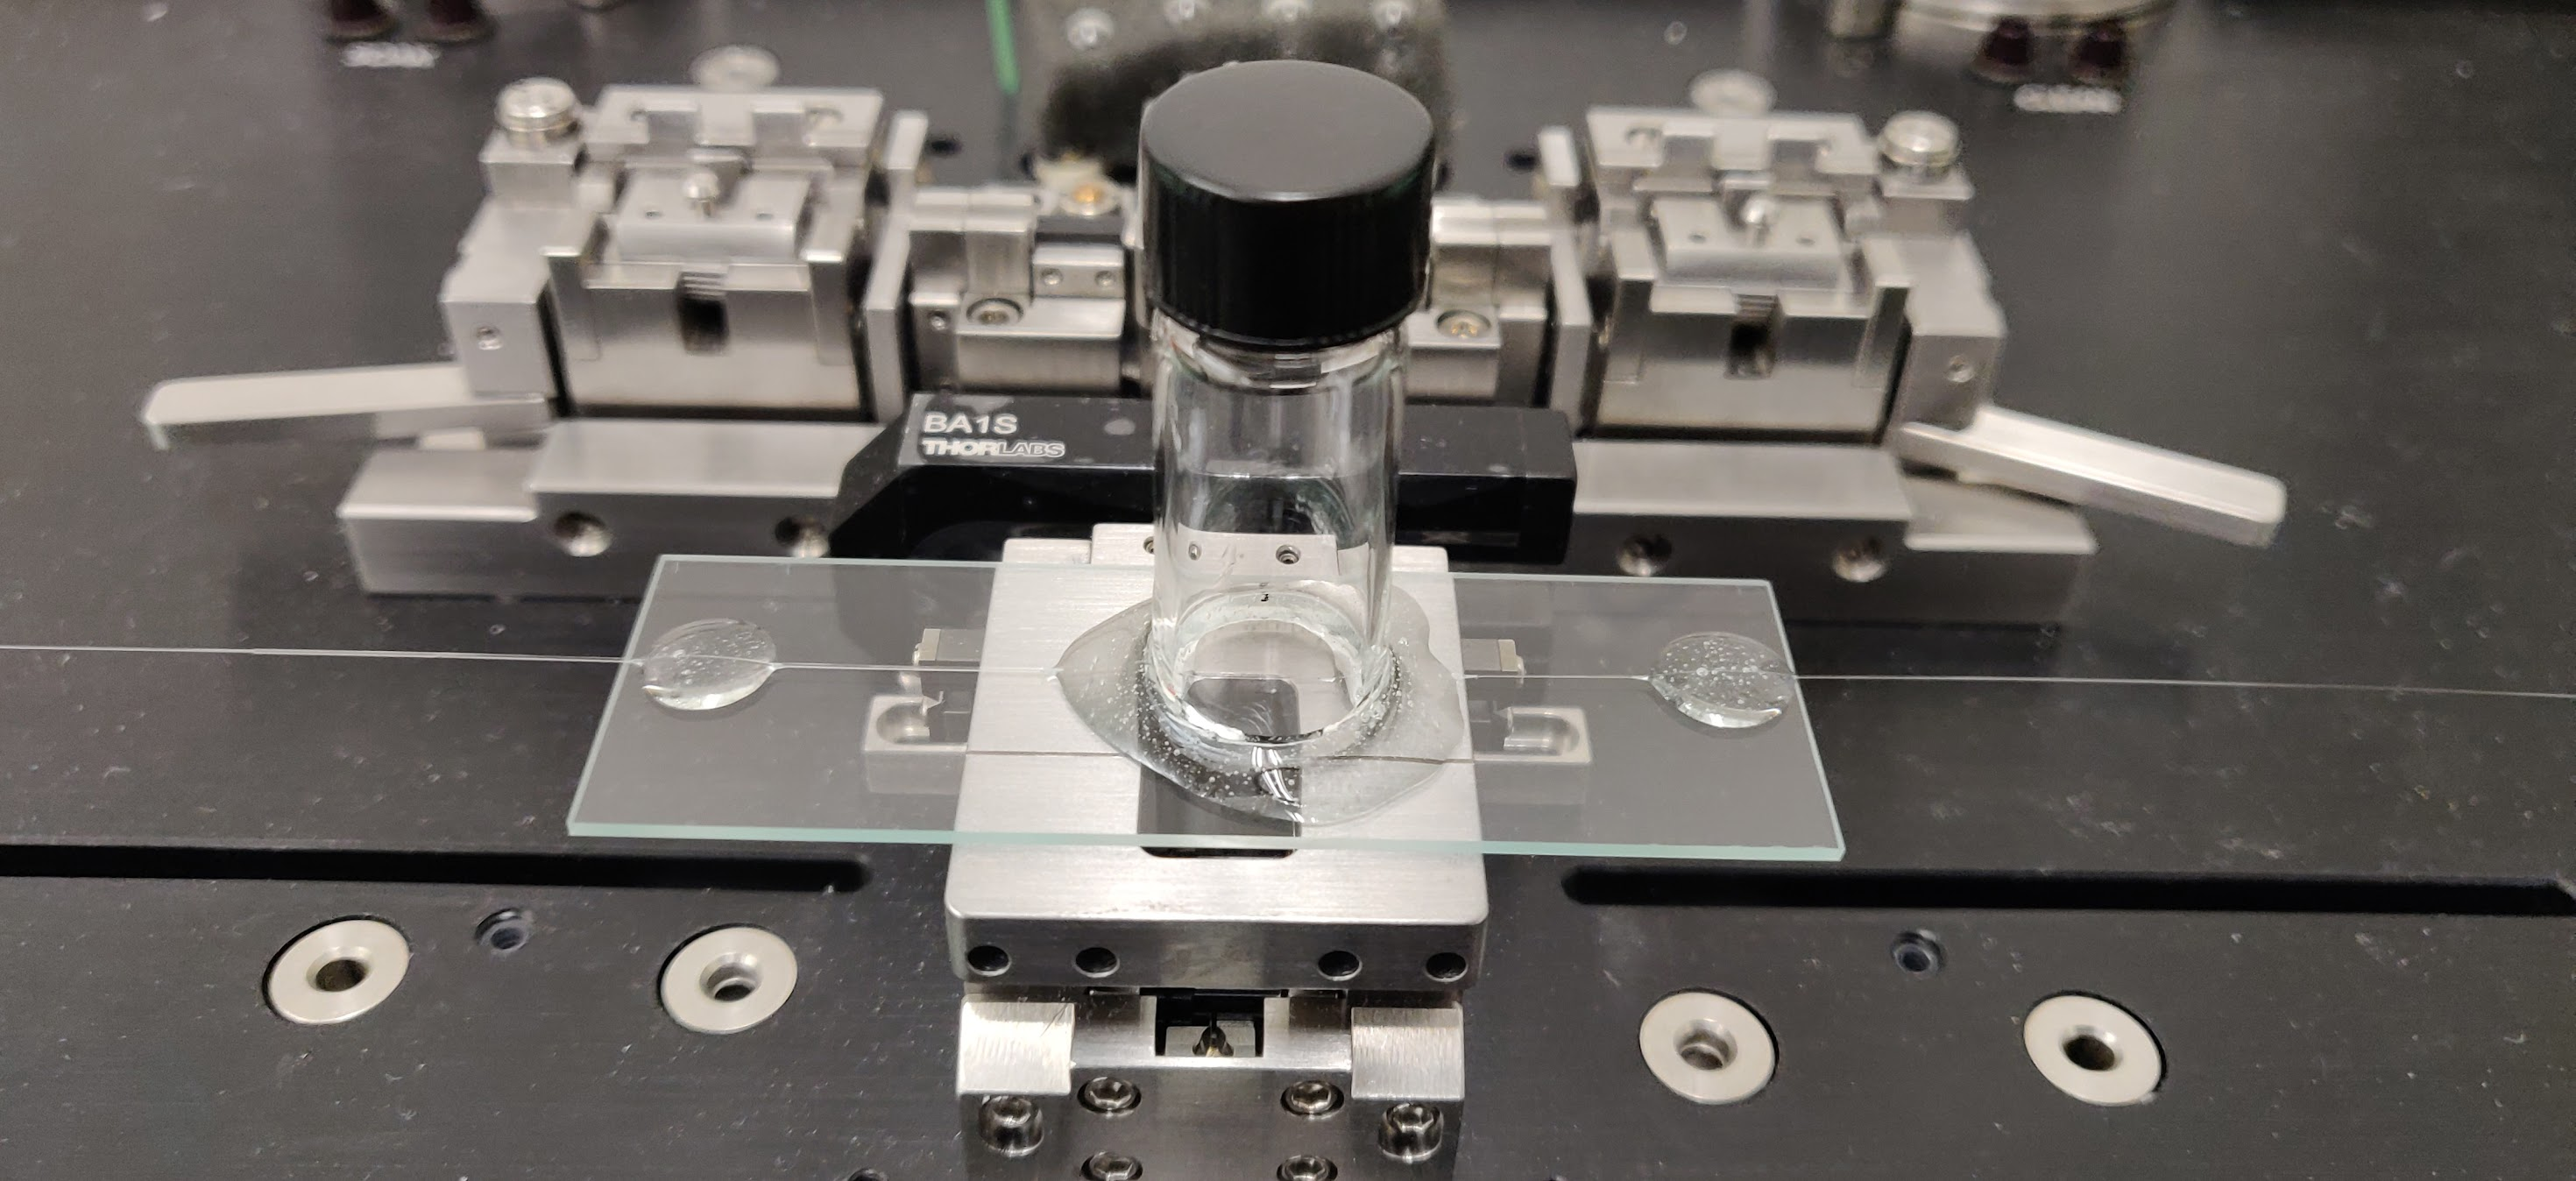
\includegraphics[width=\textwidth]{figs/2-Cooling/successfullyBuiltSplice.jpg}
  \caption{Picture of a complete splice assembly (Section~\ref{Cooling:Appendix:subsec:Reservoir Assembly}). The hardened epoxy around the base of the vial securely holds the cut and notched vial onto the slide, forming a sealed reservoire around the critical splice. The reservoire is later filled with liquid \ce{CS2} by easy removal of the screw-off cap in order to submerge the critical splice and begin the filling process of the hollow-core fiber via capilary action.}
  \label{fig:successfully build splice}
\end{figure}

Upon completing the angle splice, the fiber assembly needed to be moved gently off the splicer onto the prepared microscope slide:

\begin{enumerate}
	\item Release and Stabilization: With the splicer’s vacuum pump still on to hold the splice securely, the magnetic latches clamping the fiber on either side of the splice to the translation/rotation stages were carefully lifted. Tweezers were used to remove any fiber “flags,” and wooden craft sticks helped lift the fibers from the block grooves to free the fiber from any stuck position within the grooves.
  \item Vacuum Shut-Off: The splicer's vacuum pump was switched off and the vacuum seal securing the fibers on either end of the splice was allowed to gradually release as air slowly equilibrated the pressure differential. The splice head and camera assembly remained overtop the splice for monitoring the camera feed on the computer screen. After approximately five minutes the camera feed would show the splice quickly move out of focus, indicating that the entire length of fiber was free and ready to be handled.
	\item Placement on the Slide: With the splice head lifted, the slide was positioned directly in front of the splice and the fiber was transferred carefully in a smooth motion. Two small drops of epoxy were placed on each side of the splice region to tack the fiber down. This was allowed to cure for at least five minutes.
\end{enumerate}

\begin{figure}[t]
  \centering
  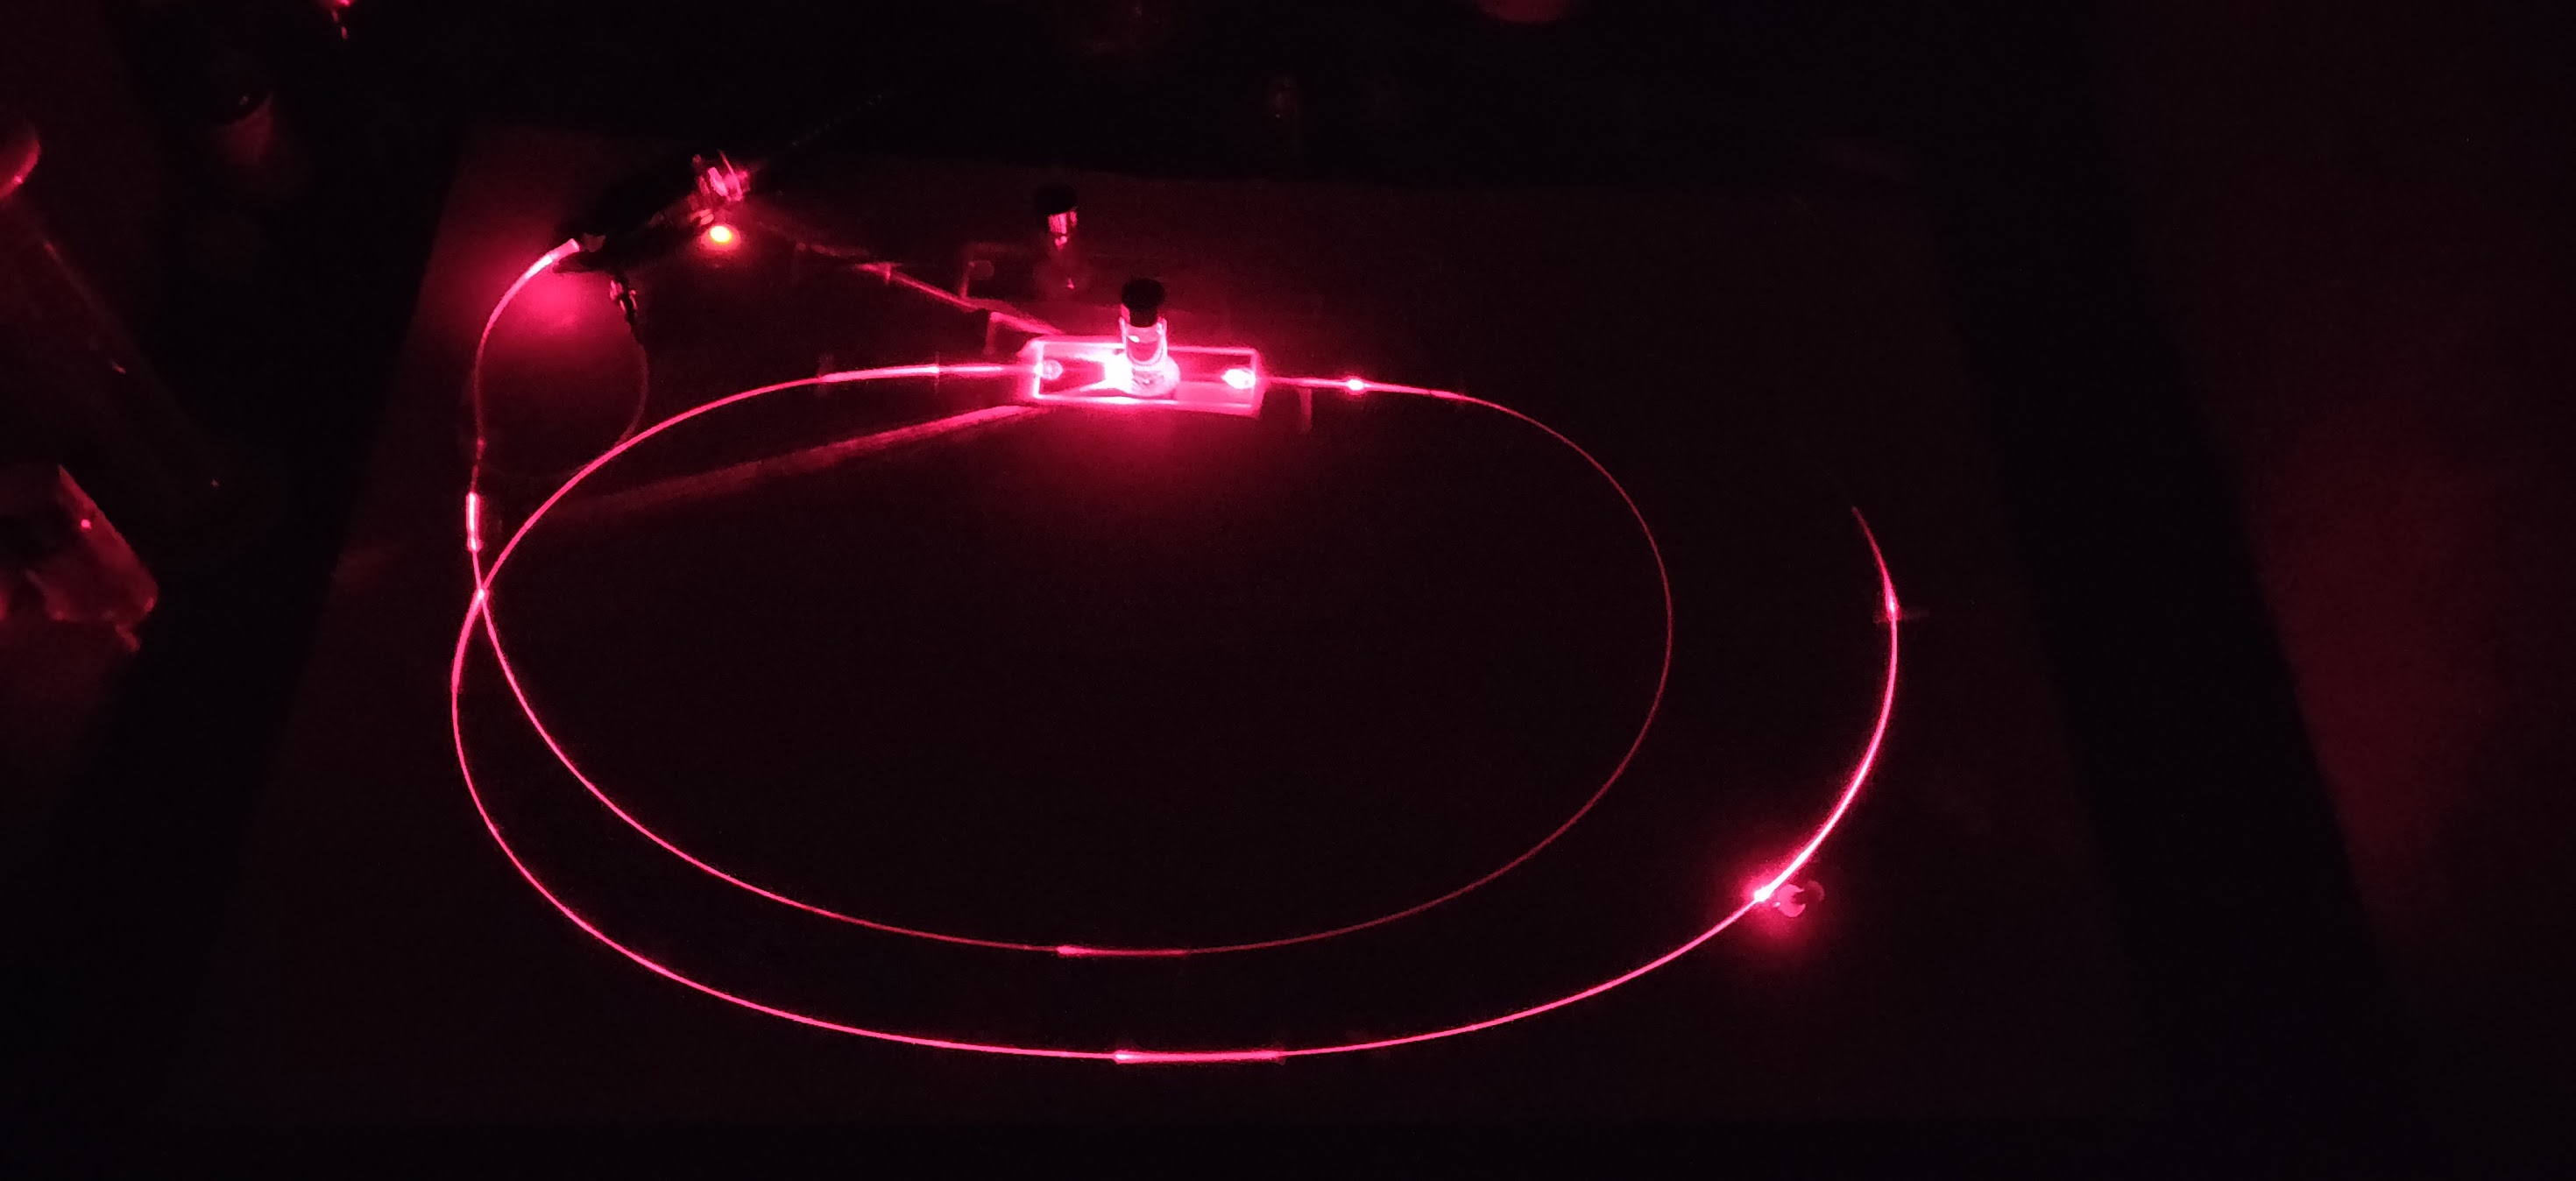
\includegraphics[width=\textwidth]{figs/2-Cooling/redLightWithThumbTackWholeSample.jpg}
  \caption{Picture of a complete sample under the fume hood with lights dimmed and red laser light injected into the end of the sample for monitoring (Section~\ref{Cooling:Appendix:subsec:Filling with CS2}). The red light is partially guided along the length of fiber which has filled with liquid \ce{CS2} and a thumb tack marks the progress of the \ce{CS2}-air interface.}
  \label{fig:red Light with Thumb Tack Whole Sample}
\end{figure}

The splice region was enclosed in a glass vial to protect the hollow-core’s interior and to facilitate later filling with liquid:

\begin{enumerate}
	\item Positioning the Vial: The prepared vial was placed over the splice region by sliding one straddle-gap around the fiber first, then tilting it so the second gap aligned. Gloves were worn to prevent transferring skin oils onto the vial.
	\item Epoxy Sealing: A fresh mixture of two-part epoxy was prepared in roughly equal proportions and thoroughly mixed for 10–15 seconds to ensure a uniform bond. Generous epoxy was applied around the vial’s perimeter where it contacted the slide. Care was taken to avoid epoxy wicking into the splice itself. The assembly was then left undisturbed for at least five minutes to cure.
\end{enumerate}

\begin{figure}[t]
    \centering
    \begin{subfigure}[b]{0.49\textwidth}
        \centering
        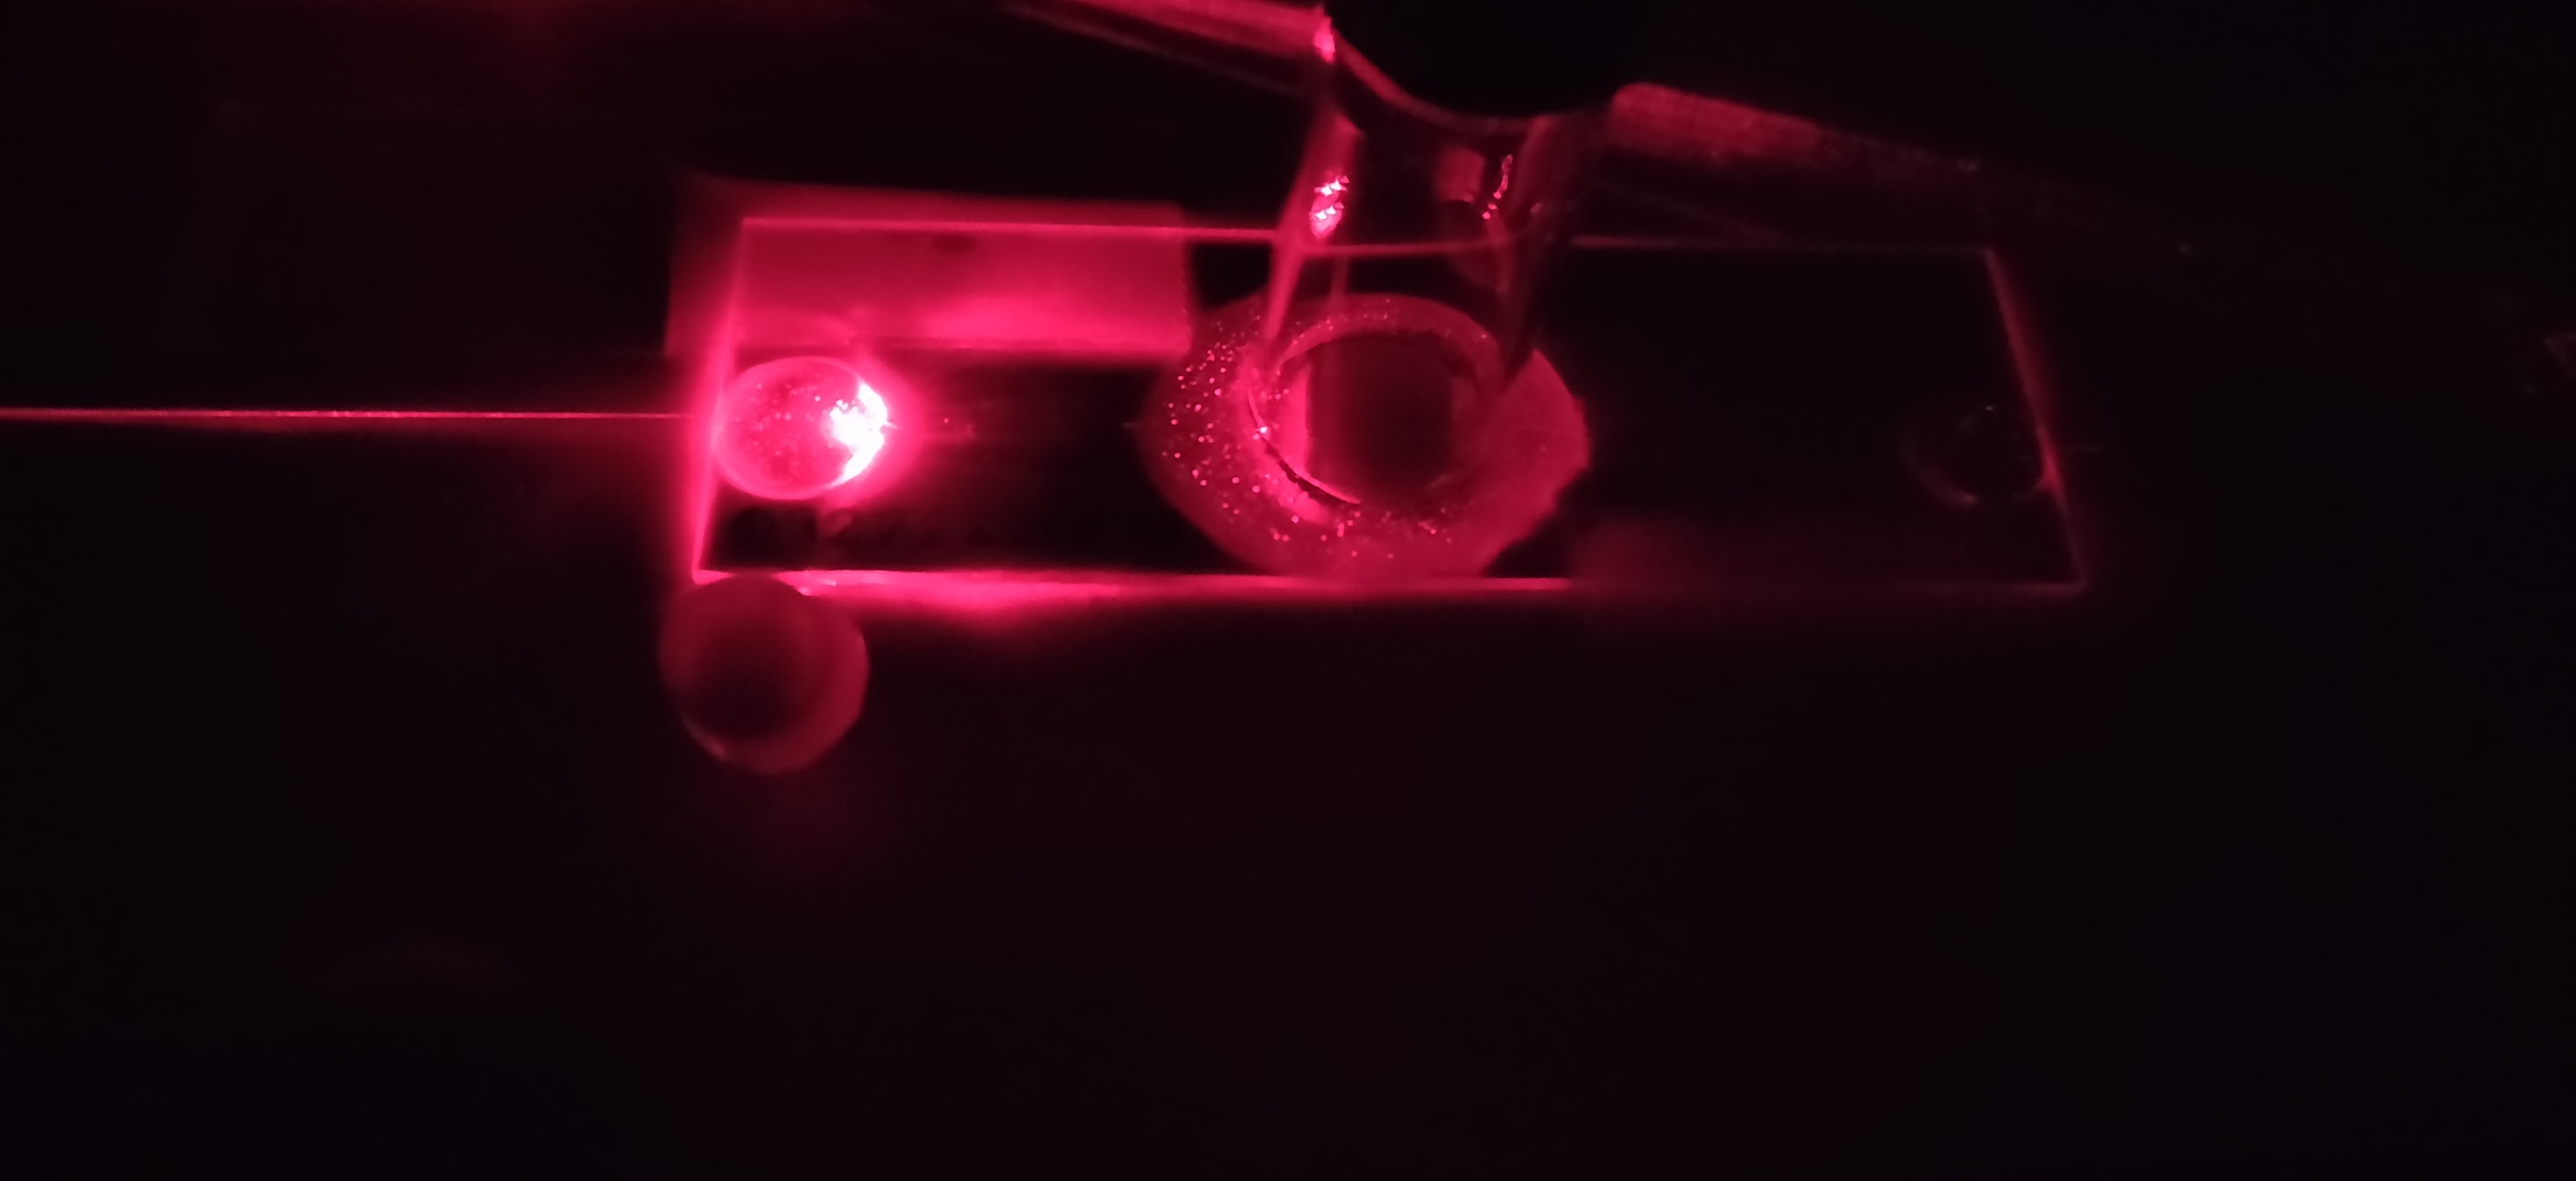
\includegraphics[width=\textwidth]{figs/2-Cooling/CS2NearlyReached.jpg}
        \caption{}
        \label{fig:Cooling:CS2 Nearly Reached}
    \end{subfigure}
    \hfill
    \begin{subfigure}[b]{0.49\textwidth}
        \centering
        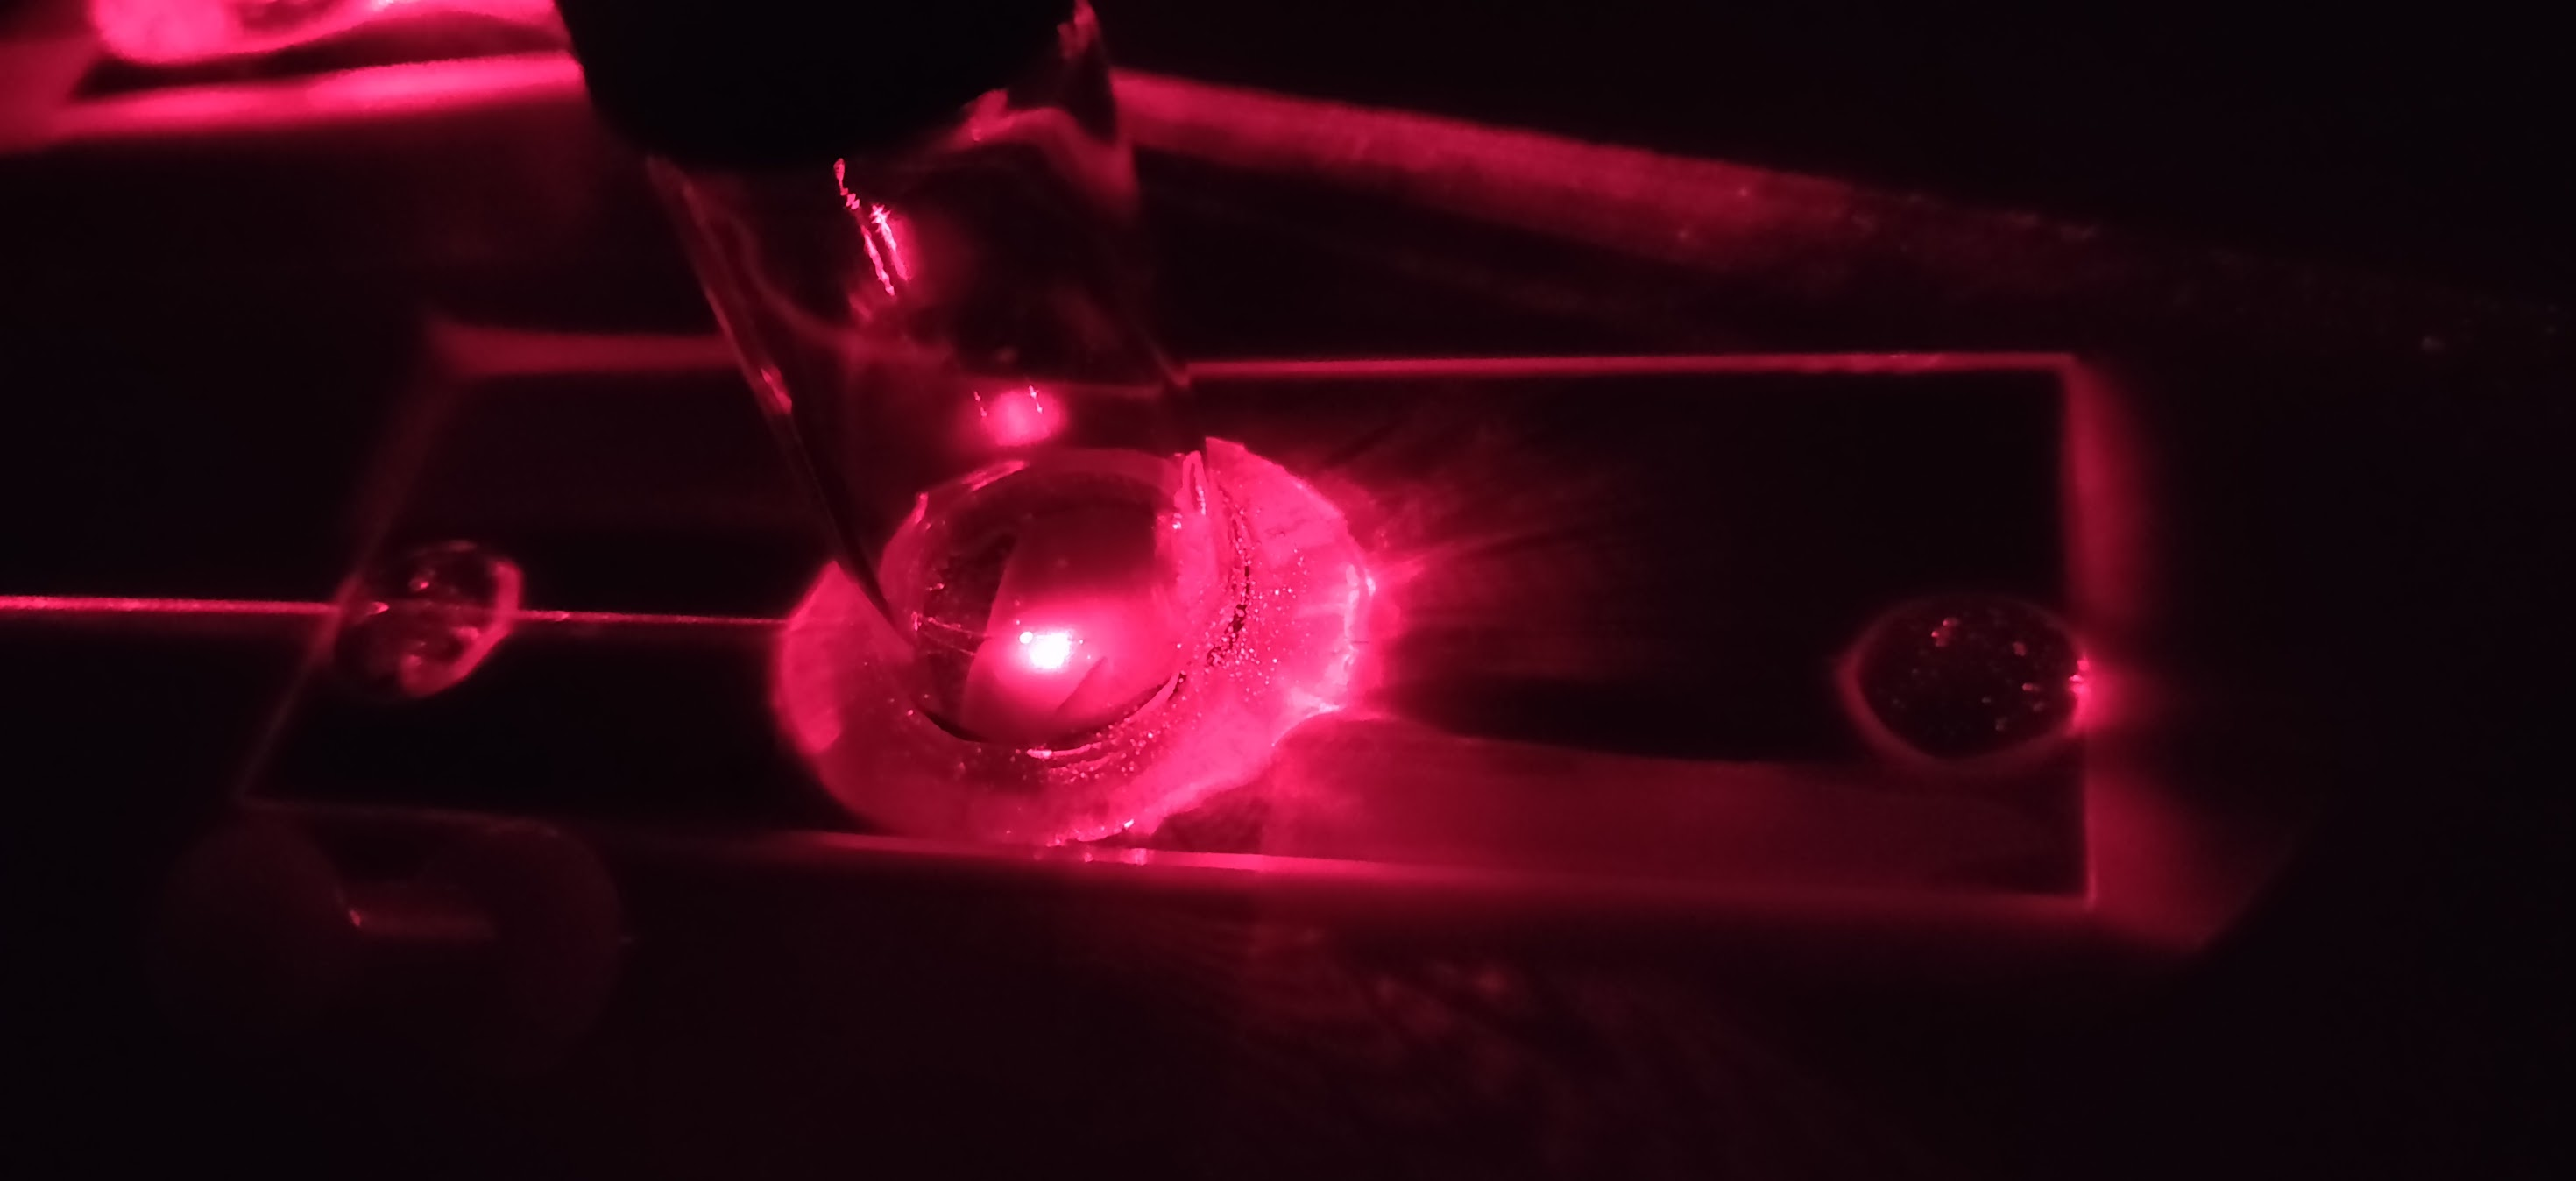
\includegraphics[width=\textwidth]{figs/2-Cooling/CS2Reached.jpg}
        \caption{}
        \label{fig:Cooling:CS2 Reached}
    \end{subfigure}
    \caption{Images of an \ac{LCOF} sample in the filling process (Section~\ref{Cooling:Appendix:subsec:Filling with CS2}). Figure (a) shows the \ce{CS2}-air interface a few centimeters from the end of the length hollow-core fiber, indicated by the red dot of scattered light just underneath the epoxy tack. From this position, the meniscus will typically reach the exit splice in approximately 4 hours. Figure (b) shows evidence of a fully-filled \ac{LCOF} sample, indicated by the red dot of scattered light having reached the exit splice. If the pictured reservoire were to be filled prematurely, an air bubble would be locked in, reducing full transmission through the sample to nearly 0\%.}
    \label{fig:Cooling:red dot monitoring near the end}
\end{figure}

Once the epoxy had set, the slide was labeled with the date, splice reference, and relevant notes using a marker. For long-term handling, the slide and its fibers were taped to a poster board to facilitate transport and prevent accidental breakage from jostling. This procedure ensured a robust, low-loss transition from \ac{SMF-28} to \ac{UHNA7} to the hollow-core fiber. The careful cleaning steps, controlled splicing environment with argon shielding, and meticulous handling minimized the risk of fiber breakage and guaranteed a clean optical interface. Encapsulating the splice with a modified glass vial on a microscope slide allowed easy manipulation of the hollow core’s environment, which was crucial for subsequent liquid filling and optical characterization experiments.

Finally, this entire procedure was repeated on the opposite side of the hollow-core fiber to complete the \ac{LCOF} assembly. Each splice was carefully optimized to be robust enough to guide light but also unfused enough to allow \ce{CS2} to enter the hollow core via capillary action.

\subsection{Filling with Carbon Disulfide}
\label{Cooling:Appendix:subsec:Filling with CS2}

Once both ends of the hollow-core fiber were successfully spliced to their respective fiber pigtails, the next critical step involved filling the hollow core with carbon disulfide. Because \ce{CS2} is highly volatile and poses health risks if inhaled, all operations were carried out in a fume hood with proper protective equipment.

The prepared \ac{LCOF} sample, securely taped to a poster board, was transferred to the fume hood. A small red laser source was connected to the input pigtail; this red beam served as an in situ indicator of the fluid-filling front. The vial on the input side was uncapped, and the vial on the opposite side was loosened to prevent pressure buildup within the fiber. This arrangement ensured that as \ce{CS2} entered the hollow core, displaced air could escape through the opposite vial, allowing continuous capillary flow.

To deliver the \ce{CS2}, a syringe was first used to extract an adequate volume from a sealed supply bottle. The needle tip was then removed and replaced with a micron-level particulate filter, thereby minimizing the introduction of debris that could obstruct the hollow core. By gently angling the syringe, \ce{CS2} was dispensed along the interior wall of the vial rather than dripping directly onto the delicate splice region. This careful approach reduced mechanical shocks, which could otherwise fracture or misalign the newly formed splice. Once the vial was filled, it was recapped promptly to prevent evaporation.

If a given splice was imperfect—fully sealed at the fiber core rather than partially open—it prevented \ce{CS2} from flowing in. Under these circumstances, no visible progression of the fluid meniscus would appear in the red laser beam path, confirming an unsuccessful splice. In contrast, if the splice was partially open, capillary action would begin immediately, typically drawing \ce{CS2} several centimeters into the hollow core within seconds. The interface between the \ce{CS2} and the air still occupying the rest of the fiber showed up as a faintly scattering “dot” in the path of the red beam. By darkening the room, this dot could be easily observed and tracked. Once the fiber was fully filled, the second vial was also filled with filtered \ce{CS2}, then capped. If the second reservoir was filled prematurely, an air bubble would be trapped in the final short length of hollow-core fiber and the resulting transmission through the full length of the \ac{LCOF} would be reduced to nearly 0\%.

\begin{figure}[t]
    \centering
    \begin{subfigure}[b]{0.49\textwidth}
        \centering
        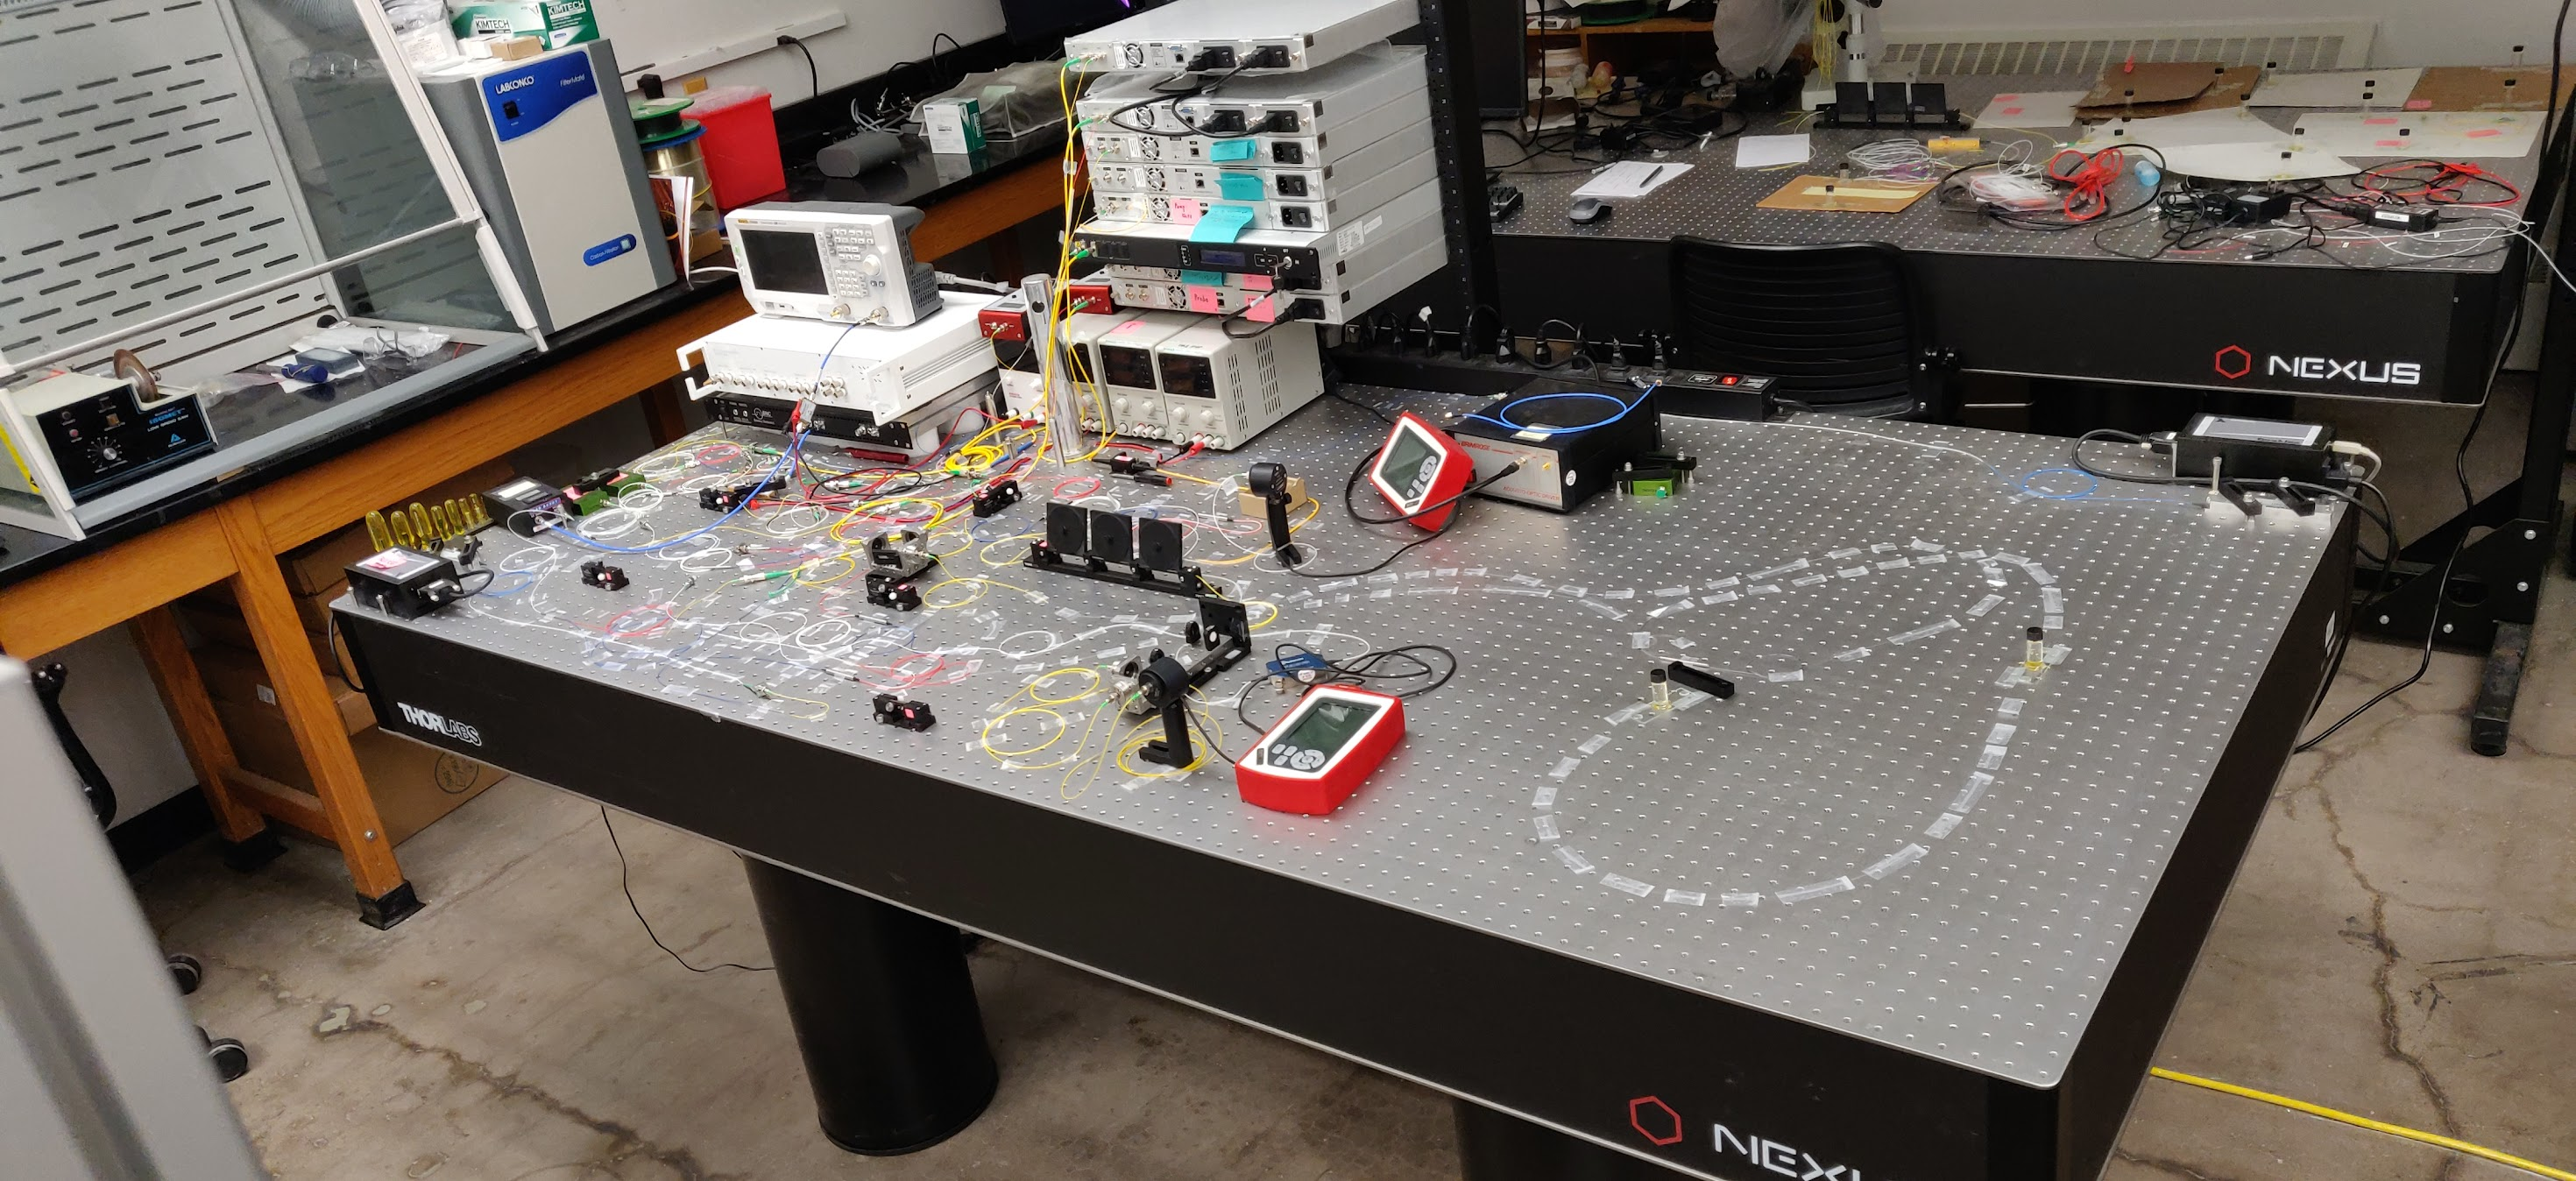
\includegraphics[width=\textwidth]{figs/2-Cooling/fullSampleTapedToOpticalTable.jpg}
        \caption{}
        \label{fig:Cooling:Full Sample Taped on Table}
    \end{subfigure}
    \hfill
    \begin{subfigure}[b]{0.49\textwidth}
        \centering
        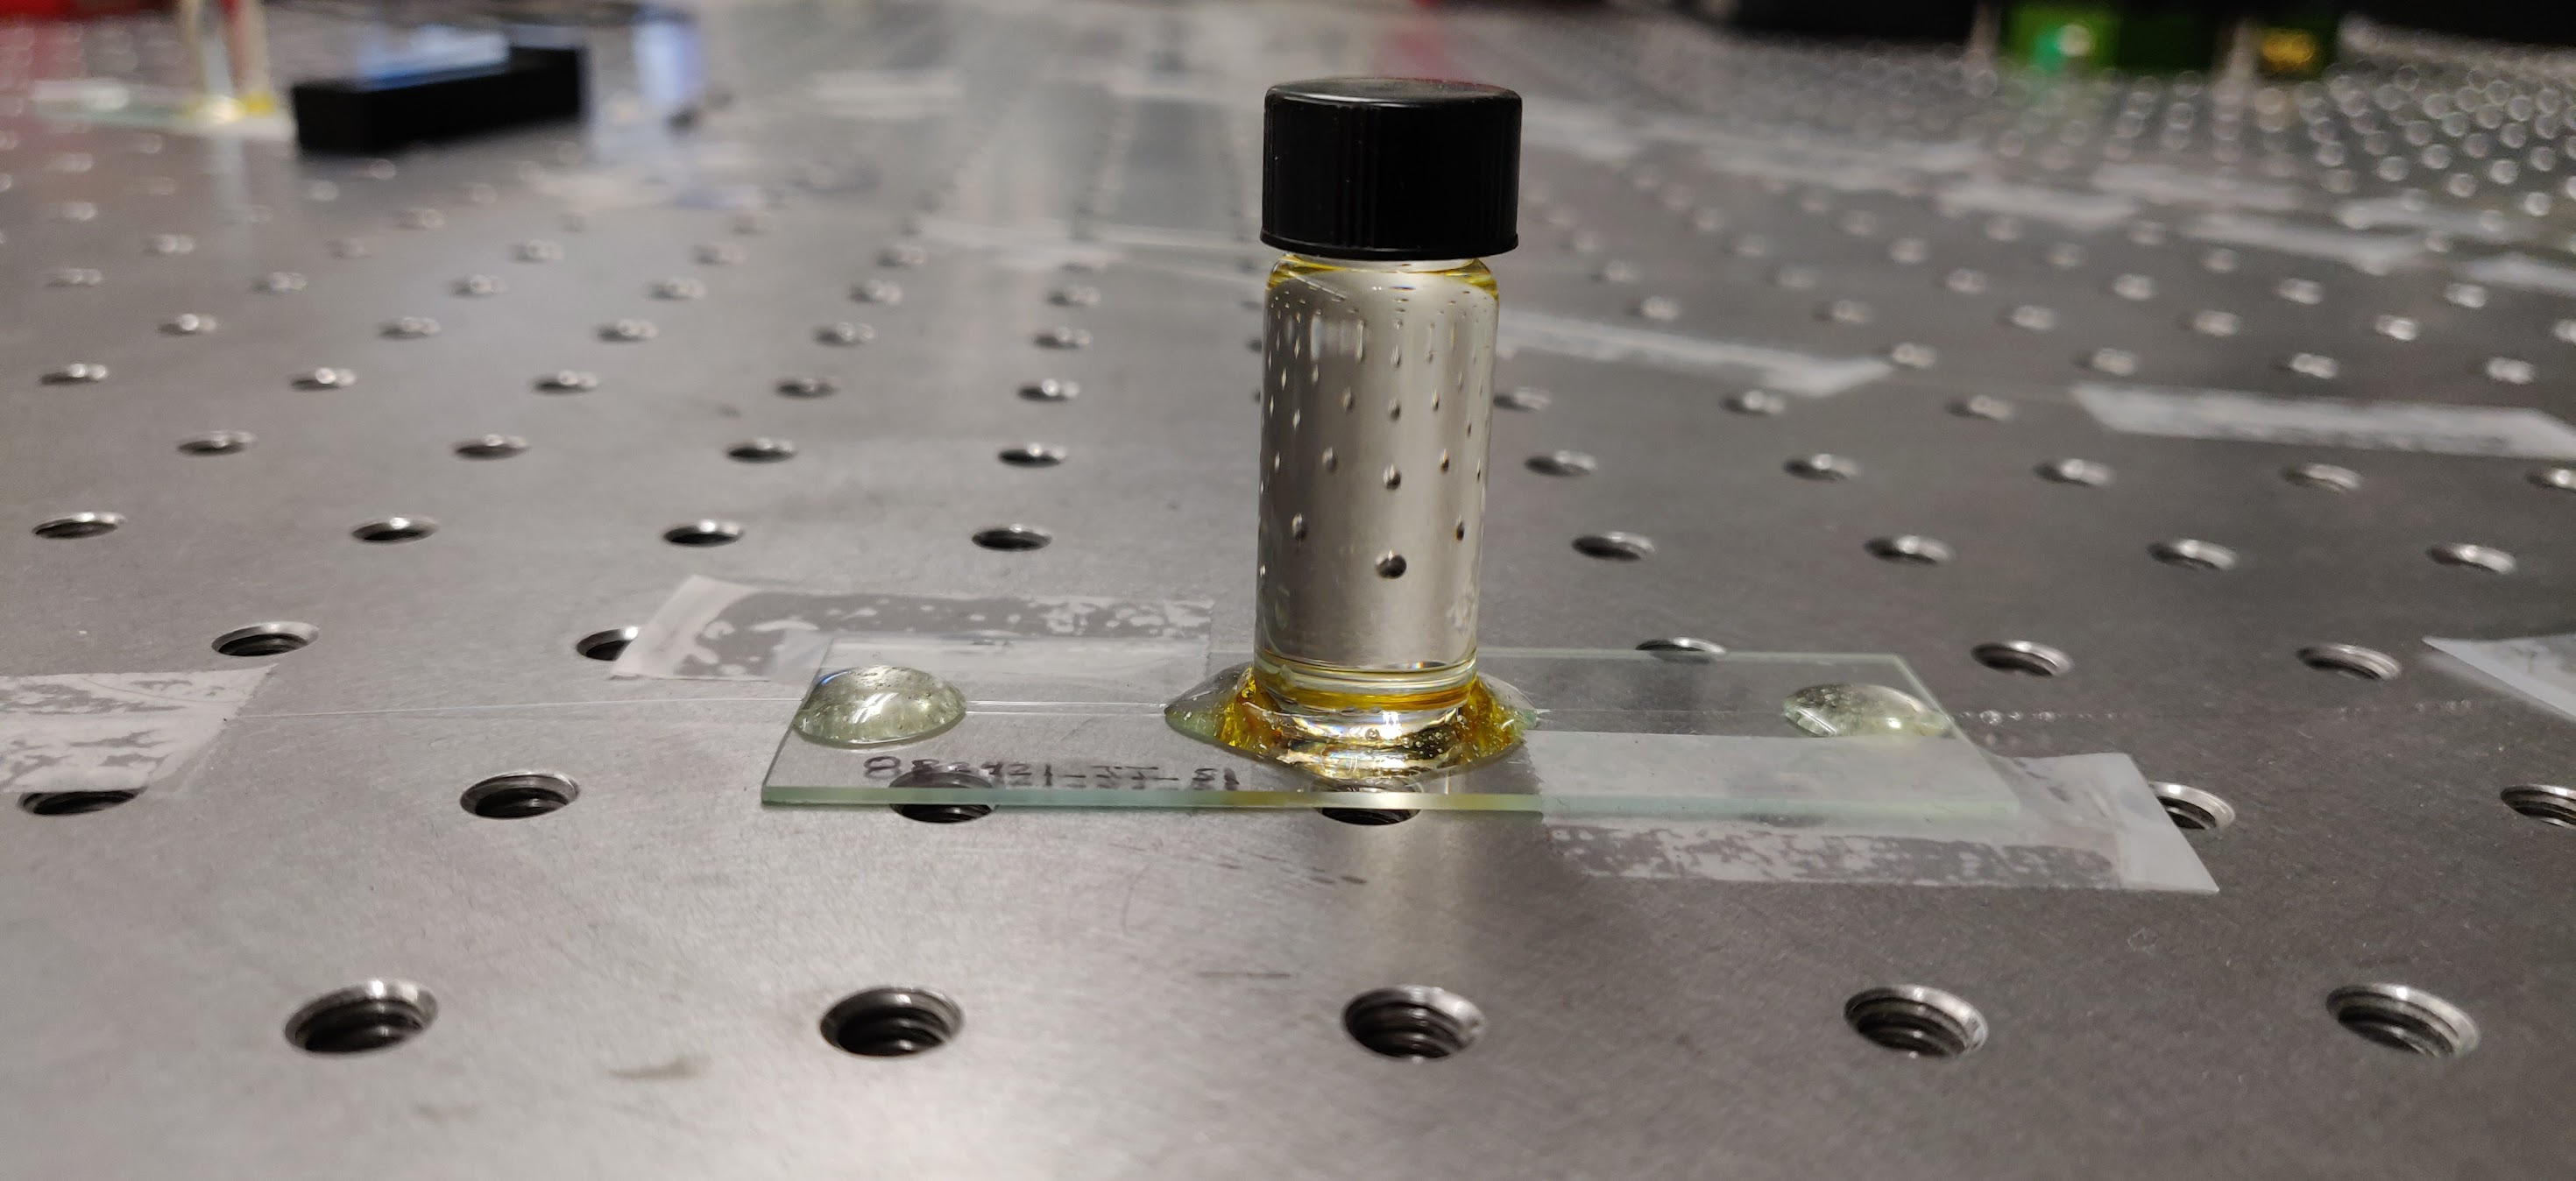
\includegraphics[width=\textwidth]{figs/2-Cooling/spliceTapedDirectlyOnOpticalTable.jpg}
        \caption{}
        \label{fig:Cooling:Splice Taped on Table}
    \end{subfigure}
    \caption{Images of a fully finished \ce{CS2}-\ac{LCOF} sample (Section~\ref{Cooling:Appendix:subsec:Typical Optical Performance}). Figure (a) shows a sample secured with tape to an optical table and integrated into an optical setup. Liberal use of tape ensured the safety of the sample as well as reduced vibrations and minimized changes in the polarization of light travelling through the sample. Figure (b) shows one splice assembly secured directly to the optical table via tape. Transfer of all parts of the sample from the poster board directly onto the optical table proved critical for eliminating noise and polarization drift issues with the pump-probe experiment.}
    \label{fig:Cooling:LCOF Taped on Table}
\end{figure}

Figure~\ref{fig:red Light with Thumb Tack Whole Sample} shows a picture of a sample in the process of filling with \ce{CS2}. Progress is marked by a thumbtack next to the \ce{CS2}-air interface. With the lights turned off, the dot of scattered light at this interface was a reliable visible indicator. Figures~\ref{fig:Cooling:CS2 Nearly Reached} and \ref{fig:Cooling:CS2 Reached} show images of a sample that has nearly finished and fully finished filling, respectively. The filling state captured by Figure~\ref{fig:Cooling:CS2 Nearly Reached} indicates a likely time to finish filling of approximately 4 hours.

\subsection{Typical Optical Performance}
\label{Cooling:Appendix:subsec:Typical Optical Performance}

Optical transmission at each splice typically ranged from 5–25\%. The final \ac{LCOF} used to gather the experimental results published in the paper associated with this chapter achieved full throughput transmission of about 17\%. This suggests each splice individually offered an average of approximately 41\% transmission of the incident light, assuming each splice provided equal transmission. In the demonstration of optomechanical cooling of traveling-wave phonons in this \ac{LCOF}, the light collected at the detector is backscattered within the sample and thus passes back through the same splice that the incident pump light enters through. This round-trip backscattered \ac{LCOF} transmission was treated as approximately equal to the full throughput transmission monitored to be exiting the sample, as light passes through two splices of assumed equal transmission in each case.

Figure~\ref{fig:Cooling:LCOF Taped on Table} shows two images of a complete \ac{LCOF} secured to an optical table with Scotch tape and integrated into an optical setup. In later stages of experimentation if was discovered that a large amount of noise and changes in polarization of the light passing through the sample would be incurred if the \ac{LCOF} were left attached to the poster board used in fabrication and transport. Despite taping all edges of the poster board securely down onto the optical table, minor flexing of the board from small temperature and humidity changes or air drafts in the room caused sufficient instability in the signal to delay successful data collection for the pump-probe experiment (Section~\ref{Cooling:subsec:ExperimentBResults}).

Over periods of days, some evaporation was inevitable; replenishing the vials every two to three days extended the operational lifetime of the sample. Despite occasional epoxy degradation at the splice site, which might reduce forward transmission, the backscattering experiments remained unaffected except for a loss of forward transmission monitoring. In most cases, weeks-long sample preservation and continued experimentation was feasible with proper maintenance.

\section{Improvements in Yield and Efficiency of \acs{LCOF} Samples}
\label{Cooling:Appendix:sec:ImprovementsinYieldandEfficiencyofLCOFSamples}

A key refinement that greatly improved sample fabrication success rates was the adoption of extremely careful post-splice handling. Previously, standard procedure was to lift the newly spliced fiber assembly without ensuring that each side was completely free of the splicer’s grooves. This led to abrupt bending or sudden “snapping” out of the clamp grooves, which almost invariably broke delicate splices that were only partially fused. The implementation of several measures helped to avoid this failure mode. First, folded-paper “sawhorses” and two small Kimwipe boxes on each side of the splice were placed to support the fibers and reduce vibration or flexing. Before switching off the vacuum seal, the clamp latches were gently lifted and small wooden sticks were used to ease the fibers out of the translation/rotation block grooves, ensuring there was no latent twisting or bending. Throughout these steps, the fibers were kept as close as possible to their natural resting position, minimizing stress that would be transferred to the just-completed splice. This careful approach not only reduced the chance of breakage but also allowed for the feasibility of splices that remained sufficiently “open” for \ce{CS2} to enter the hollow core, substantially increasing the proportion of successfully filled samples.

In using the slow-rotation saw to cut and form notches in the glass vial, simple improvements in notch geometry greatly reduced breakage of splices while placing the vial on the slide overtop the delicate splice, and straddling the fibers on either side. Cutting notches to be \(\sim\SI{1}{\centi\meter}\) (10-20 times the width of the fiber) reduced the risk of inadvertently contacting the fibers and breaking the delicate splice during vial placement. Additionally, cutting the notches to be shallow (approximately 5 times the width of the fiber) prevented epoxy from running through the notch and sealing the splice. Previous standard procedure were opposite to this geometry as a natural result of the narrow width of the saw blade and the depth to which it could easily be allowed to cut.

A key innovation in the filling procedure was performing a long observation of the filling process for one sample. Previous standard procedure was to stop monitoring after 8 or 12 hours, assuming the fill process had ceased or completed but subsequently reversed if the fluid had not reached the far end by that time. Through extended trials, it was discovered that in successful splices, the fill front progresses at a nonlinear, steadily decreasing rate, and that a one-meter fiber segment migh take more than 24 hours to completely fill. In one particularly instructive case, continuous monitoring for 27 hours without leaving the room as a sample filled confirmed that the \ce{CS2} front never reversed; it merely advanced extremely slowly in the final length to reach the other end. Alarms were set for inspection every 90 minutes throughout the night in the final hours of monitoring the sample under the fume hood. Having observed and documented this behavior, the standard practice became allowing the sample to sit undisturbed for at least a full day or more, ensuring the fiber was completely saturated before concluding success or failure. This observation effort and resulting insight halted the regular production of significant waste of both material and time in the fabrication process of \ac{LCOF} samples.

A final insight that improved the yield of successfully filled samples and mitigation of wasted materials was selecting the “less certain” end of a prepared sample for filling with \ce{CS2}. If that splice was sealed, only that end would need to be re-fabricated. Collectively, these simple method improvements in sample fabrication led to significantly shorter fabrication times and dramatically reduced material waste. Hollow-core fibers, which cost on the order of ten dollar per meter, were previously scrapped in large quantities when deemed “dead.” By implementing patient monitoring, careful handling, and mindful filling procedures each length of fiber was used more efficiently, saving significant time and expense while producing more effective samples.

\newpage

\section{Tabulated Fit and Uncertainty Values Derived from the Experimental Data}
\label{Cooling:Appendix:sec:Tabulated Fit and Uncertainty Values Derived From the Experimental Data}

\subsection{Experiment~A Tabulated Values}
\label{Cooling:Appendix:subsec:Experiment A Tabulated Values}

%======================================================================
% Anti-Stokes Table
%======================================================================
\begin{table}[h!]
  \centering
  \caption{Measured anti-Stokes parameters for Experiment~A. Here \(P_{\mathrm{P}}\) is the nominal pump power, measured via a 1\% tap just prior to launching into the LCOF, and \(P_{\mathrm{Intra}}\) is the power actually guided within the fiber. Amplitude, Linewidth, Center, and Offset are the peak spectral density, FWHM linewidth, center frequency, and vertical baseline offset, respectively, obtained from a Lorentzian fit of the data. Uncertainties are 1\(\sigma\).}
  \label{tab:Cooling:Experiment A anti-Stokes}
  \begin{tabular}{
      S[table-align-uncertainty]   % Pump Power
      S[table-align-uncertainty]   % Intrafiber
      S[table-align-uncertainty]   % Amplitude
      S[table-align-uncertainty]   % Linewidth
      S[table-align-uncertainty]   % Center
      S[table-align-uncertainty]   % Offset
    }
    \toprule
		\multicolumn{1}{c}{\(\mathbf{P}_{\mathrm{\textbf{P}}}\)} &
    \multicolumn{1}{c}{\(\mathbf{P}_{\mathrm{\textbf{Intra}}}\)} &
    \multicolumn{1}{c}{\textbf{Amplitude}} &
    \multicolumn{1}{c}{\textbf{Linewidth}} &
    \multicolumn{1}{c}{\textbf{Center}} &
    \multicolumn{1}{c}{\textbf{Offset}} \\
    \multicolumn{1}{c}{(\si{\milli\watt})} &
    \multicolumn{1}{c}{(\si{\milli\watt})} &
    \multicolumn{1}{c}{(\si{\micro\volt})} &
    \multicolumn{1}{c}{(\si{\mega\hertz})} &
    \multicolumn{1}{c}{(\si{\giga\hertz})} &
    \multicolumn{1}{c}{(\si{\micro\volt})} \\
    \midrule

		\num{10.00} & \num{4.12} & \num{3.015(0.0043)} & \num{97.315(0.119)} & \num{2.2690(0.0001)} & \num{-0.006(0.0017)} \\
    \num{30.00} & \num{12.37} & \num{8.747(0.0061)} & \num{99.097(0.0547)} & \num{2.2690(0.0000)} & \num{0.015(0.0019)} \\
    \num{50.00} & \num{20.62} & \num{14.224(0.0097)} & \num{99.793(0.0449)} & \num{2.2690(0.0000)} & \num{0.032(0.0021)} \\
    \num{70.00} & \num{28.86} & \num{19.123(0.0167)} & \num{101.147(0.0508)} & \num{2.2690(0.0000)} & \num{0.015(0.0027)} \\
    \num{90.00} & \num{37.11} & \num{24.919(0.0116)} & \num{100.907(0.0315)} & \num{2.2680(0.0000)} & \num{0.039(0.0025)} \\
    \num{110.00} & \num{45.35} & \num{31.265(0.0174)} & \num{102.325(0.0334)} & \num{2.2690(0.0000)} & \num{0.029(0.0028)} \\
    \num{130.00} & \num{53.60} & \num{36.061(0.0178)} & \num{102.454(0.0290)} & \num{2.2690(0.0000)} & \num{0.016(0.0027)} \\
    \num{150.00} & \num{61.85} & \num{41.590(0.0219)} & \num{102.547(0.0313)} & \num{2.2690(0.0000)} & \num{0.118(0.0033)} \\
    \num{170.00} & \num{70.09} & \num{46.782(0.0220)} & \num{103.267(0.0287)} & \num{2.2690(0.0000)} & \num{0.086(0.0034)} \\
    \num{190.00} & \num{78.34} & \num{51.855(0.0273)} & \num{105.023(0.0314)} & \num{2.2690(0.0000)} & \num{-0.071(0.0038)} \\
    \num{210.00} & \num{86.59} & \num{57.035(0.0236)} & \num{105.131(0.0255)} & \num{2.2690(0.0000)} & \num{0.058(0.0037)} \\
    \num{230.00} & \num{94.83} & \num{61.421(0.0260)} & \num{105.634(0.0268)} & \num{2.2690(0.0000)} & \num{0.093(0.0040)} \\
    \num{250.00} & \num{103.08} & \num{66.638(0.0378)} & \num{105.825(0.0328)} & \num{2.2690(0.0000)} & \num{0.148(0.0049)} \\
    \num{270.00} & \num{111.32} & \num{70.627(0.0439)} & \num{106.417(0.0363)} & \num{2.2690(0.0000)} & \num{0.205(0.0059)} \\
    \num{290.00} & \num{119.57} & \num{74.680(0.0403)} & \num{106.315(0.0333)} & \num{2.2690(0.0000)} & \num{0.314(0.0062)} \\

    \bottomrule
  \end{tabular}
\end{table}

%======================================================================
% Stokes Table
%======================================================================
\begin{table}[h!]
  \centering
  \caption{Measured Stokes parameters for Experiment~A, in the same format as Table~\ref{tab:Cooling:Experiment A anti-Stokes}.}
  \label{tab:Cooling:Experiment A Stokes}
  \begin{tabular}{
			S   % Pump Power
			S   % Intrafiber
			S[table-align-uncertainty]   % Amplitude
			S[table-align-uncertainty]   % Linewidth
			S[table-align-uncertainty]   % Center
			S[table-align-uncertainty]   % Offset
    }
    \toprule
		\multicolumn{1}{c}{\(\mathbf{P}_{\mathrm{\textbf{P}}}\)} &
    \multicolumn{1}{c}{\(\mathbf{P}_{\mathrm{\textbf{Intra}}}\)} &
    \multicolumn{1}{c}{\textbf{Amplitude}} &
    \multicolumn{1}{c}{\textbf{Linewidth}} &
    \multicolumn{1}{c}{\textbf{Center}} &
    \multicolumn{1}{c}{\textbf{Offset}} \\
    \multicolumn{1}{c}{(\si{\milli\watt})} &
    \multicolumn{1}{c}{(\si{\milli\watt})} &
    \multicolumn{1}{c}{(\si{\micro\volt})} &
    \multicolumn{1}{c}{(\si{\mega\hertz})} &
    \multicolumn{1}{c}{(\si{\giga\hertz})} &
    \multicolumn{1}{c}{(\si{\micro\volt})} \\
    \midrule

    \num{10.00} & \num{4.12} & \num{3.203(0.0046)} & \num{97.252(0.1140)} & \num{2.2690(0.0001)} & \num{0.020(0.0017)} \\
    \num{30.00} & \num{12.37} & \num{9.686(0.0063)} & \num{96.817(0.0491)} & \num{2.2680(0.0000)} & \num{0.046(0.0020)} \\
    \num{50.00} & \num{20.62} & \num{15.874(0.0093)} & \num{96.837(0.0383)} & \num{2.2680(0.0000)} & \num{0.073(0.0021)} \\
    \num{70.00} & \num{28.86} & \num{21.872(0.0136)} & \num{96.943(0.0375)} & \num{2.2680(0.0000)} & \num{0.066(0.0024)} \\
    \num{90.00 } & \num{37.11} & \num{28.466(0.0141)} & \num{96.396(0.0292)} & \num{2.2680(0.0000)} & \num{0.102(0.0024)} \\
    \num{110.00} & \num{45.35} & \num{37.461(0.0191)} & \num{96.199(0.0308)} & \num{2.2680(0.0000)} & \num{0.084(0.0031)} \\
    \num{130.00} & \num{53.60} & \num{43.357(0.0259)} & \num{96.367(0.0295)} & \num{2.2680(0.0000)} & \num{0.023(0.0030)} \\
    \num{150.00} & \num{61.85} & \num{50.962(0.0218)} & \num{95.043(0.0237)} & \num{2.2680(0.0000)} & \num{0.174(0.0031)} \\
    \num{170.00} & \num{70.09} & \num{57.936(0.0287)} & \num{95.608(0.0237)} & \num{2.2680(0.0000)} & \num{0.058(0.0031)} \\
    \num{190.00} & \num{78.34} & \num{65.463(0.0358)} & \num{95.434(0.0281)} & \num{2.2680(0.0000)} & \num{0.029(0.0041)} \\
    \num{210.00} & \num{86.59} & \num{73.487(0.0351)} & \num{94.588(0.0224)} & \num{2.2680(0.0000)} & \num{0.166(0.0034)} \\
    \num{230.00} & \num{94.83} & \num{81.561(0.0431)} & \num{94.099(0.0245)} & \num{2.2680(0.0000)} & \num{0.170(0.0040)} \\
    \num{250.00} & \num{103.08} & \num{90.642(0.0559)} & \num{92.982(0.0290)} & \num{2.2680(0.0000)} & \num{0.272(0.0050)} \\
    \num{270.00} & \num{111.32} & \num{98.221(0.0433)} & \num{92.670(0.0212)} & \num{2.2680(0.0000)} & \num{0.316(0.0042)} \\
    \num{290.00} & \num{119.57} & \num{107.040(0.0543)} & \num{91.035(0.0242)} & \num{2.2680(0.0000)} & \num{0.557(0.0057)} \\

    \bottomrule
  \end{tabular}
\end{table}

\newpage

\subsection{Experiment~B Tabulated Values}
\label{Cooling:Appendix:subsec:Experiment B Tabulated Values}

%======================================================================
% Experiment B Table
%======================================================================
\begin{table}[h!]
  \centering
  \caption{Measured anti-Stokes parameters for Experiment~B. Here \(P_{\mathrm{P}}\) is the nominal pump power, measured via a 1\% tap just prior to launching into the LCOF, \(P_{\mathrm{Intra}}\) is the power actually guided within the fiber, and \(P_{\mathrm{Pr}}\) is the probe power, also measured just prior to launching into the \ac{LCOF}. Amplitude, Linewidth, Center, and Offset are the peak spectral density, FWHM linewidth, center frequency, and vertical baseline offset, respectively, obtained from a Lorentzian fit of the data. Uncertainties are 1\(\sigma\).}
  \label{tab:Cooling:Experiment B}
  \begin{tabular}{
      S[table-align-uncertainty]   % Pump Power
      S[table-align-uncertainty]   % Intrafiber
			S[table-align-uncertainty]	 % Probe Power
      S[table-align-uncertainty]   % Amplitude
      S[table-align-uncertainty]   % Linewidth
      S[table-align-uncertainty]   % Center
      S[table-align-uncertainty]   % Offset
    }
    \toprule
		\multicolumn{1}{c}{\(\mathbf{P}_{\mathrm{\textbf{P}}}\)} &
    \multicolumn{1}{c}{\(\mathbf{P}_{\mathrm{\textbf{Intra}}}\)} &
		\multicolumn{1}{c}{\(\mathbf{P}_{\mathrm{\textbf{Pr}}}\)} &
    \multicolumn{1}{c}{\textbf{Amplitude}} &
    \multicolumn{1}{c}{\textbf{Linewidth}} &
    \multicolumn{1}{c}{\textbf{Center}} &
    \multicolumn{1}{c}{\textbf{Offset}} \\
    \multicolumn{1}{c}{(\si{\milli\watt})} &
    \multicolumn{1}{c}{(\si{\milli\watt})} &
		\multicolumn{1}{c}{(\si{\milli\watt})} &
    \multicolumn{1}{c}{(\si{\micro\volt})} &
    \multicolumn{1}{c}{(\si{\mega\hertz})} &
    \multicolumn{1}{c}{(\si{\giga\hertz})} &
    \multicolumn{1}{c}{(\si{\micro\volt})} \\
    \midrule

		\num{0.00} & \num{0.00} & \num{10.00} & \num{1.849(0.0021)} & \num{96.599(0.1912)} & \num{2.270(0.0000)} & \num{0.023(0.0009)} \\
    \num{55.00} & \num{22.68} & \num{10.00} & \num{1.640(0.0068)} & \num{104.001(0.5147)} & \num{2.271(0.0001)} & \num{0.019(0.0012)} \\
    \num{110.00} & \num{45.35} & \num{10.00} & \num{1.526(0.0100)} & \num{106.850(0.7711)} & \num{2.271(0.0002)} & \num{0.020(0.0015)} \\

    \num{165.00} & \num{68.03} & \num{10.00} & \num{1.426(0.0111)} & \num{109.967(0.9950)} & \num{2.270(0.0003)} & \num{0.028(0.0017)} \\

    \bottomrule
  \end{tabular}
\end{table}


\doublespacing
\chapter{Supplementary Information for Chapter~\ref{ch:CoBS}}
\label{appendix: CoBS}
\acresetall


\section{Coupled-Wave Equations}
\label{Appendix:Coupled-Wave Equations}

Here we derive the coupled wave equations that describe coherent stimulated Brillouin scattering involving a pump, Stokes, probe, and backscattered optical field given respectively by
\\
\begin{equation}
    \tilde{E}_{P}(z,t) = A_{P}e^{i(k_{P}z - \omega_{P}t)} + c.c.,
    \label{eq:Pump optical field}
\end{equation}
\\
\begin{equation}
    \tilde{E}_{S}(z,t) = A_{S}e^{i(-k_{S}z - \omega_{S}t)} + c.c.,
    \label{eq:Stokes optical field}
\end{equation}
\\
\begin{equation}
    \tilde{E}_{Pr}(z,t) = A_{Pr}e^{i(k_{Pr}z - \omega_{Pr}t)} + c.c.,
    \label{eq:Probe optical field}
\end{equation}
\\
\begin{equation}
    \tilde{E}_{Sig}(z,t) = A_{Sig}e^{i(-k_{Sig}z - \omega_{Sig}t)} + c.c.,
    \label{eq:Signal optical field}
\end{equation}
\\
\noindent and a common acoustic field given by
\\
\begin{equation}
    \tilde{\rho}(z,t) = \rho_{0} + \rho(z,t)e^{i(qz - \Omega t)} + c.c.,
    \label{eq:acoustic field}
\end{equation}
\\
\noindent where \(\Omega = \omega_{P} - \omega_{S}\) and \(q = k_{P} - k_{S} \approx 2k_{P}\).


\subsection{Acoustic Field}
\label{Coupled-Wave Equations:Acoustic Field}

As in the case of SBS\cite{boyd2020nonlinear}, we start by assuming that the material obeys the acoustic wave equation,
\\
\begin{equation}
    \frac{\partial^{2}\tilde{\rho}}{\partial t^{2}} - \Gamma^{\prime}\nabla^{2}\frac{\partial\tilde{\rho}}{\partial t} - v_{s}^{2}\nabla^{2}\tilde{\rho} = \nabla\cdot\vec{f},
    \label{eq:acoustic wave equation}
\end{equation}
\\
\noindent where \(v_{s}\) is the sound speed in the material and \(\Gamma^{\prime}\) is a damping parameter given by
\\
\begin{equation}
    \Gamma^{\prime} = \frac{1}{\rho}\left[\frac{4}{3}\eta_{s} + \eta_{b} + \frac{\kappa}{C_{p}}(\gamma - 1)\right],
\end{equation}
\\
\noindent where \(\eta_{s}\) and \(\eta_{b}\) are the shear and bulk viscosity coefficients of the material, respectively. The source term on the right side of Equation~\ref{eq:acoustic wave equation} is the divergence of the electrostrictive force:
\\
\begin{equation}
    \vec{f} = \nabla p_{st} = \nabla \cdot \Bigg[-\frac{1}{2}\epsilon_{0}\gamma_{e}\Big(\langle\tilde{E}_{P} \cdot \tilde{E}_{S}\rangle + \langle\tilde{E}_{Pr} \cdot \tilde{E}_{Sig}\rangle\Big)\Bigg],
\end{equation}
\\
which yields, assuming the acoustic wave varies slowly in time,
\\
\begin{equation}
    \nabla\cdot\vec{f} = \epsilon_{0}\gamma_{e}q^{2}(A_{P}A_{S}^{*} + A_{Pr}A_{Sig}^{*})e^{i\Delta kz},
    \label{eq:electrostrictive force term}
\end{equation}
\\
where \(\Delta k = (k_{Pr} - k_{Sig}) - (k_{P} - k_{S})\) is the phase mismatch between the four optical fields. Only two electrostrictive terms survive after accounting for the orthogonal polarization of the pump and Stokes fields with respect to that of the probe and backscattered signal. Inserting this electrostrictive force term (Equation~\ref{eq:electrostrictive force term}) and the acoustic field (Equation~\ref{eq:acoustic field}) into the acoustic wave equation (Equation~\ref{eq:acoustic wave equation}), we find
\\
\begin{equation}
    -2i\Omega\frac{\partial\rho}{\partial t} - \Gamma^{\prime}2iq^{2}\Omega\rho - 2iqv_{s}^{2}\frac{\partial\rho}{\partial z} = \epsilon_{0}\gamma_{e}q^{2}(A_{P}A_{S}^{*} + A_{Pr}A_{Sig}^{*})e^{i\Delta kz},
\end{equation}
\\
which can be restated in terms of the Brillouin linewidth, \(\Gamma_{B} = q^{2}\Gamma^{\prime}\), as
\\
\begin{equation}
    -2i\Omega\frac{\partial\rho}{\partial t} - 2i\Omega\Gamma_{B}\rho - 2iqv_{s}^{2}\frac{\partial\rho}{\partial z} = \epsilon_{0}\gamma_{e}q^{2}(A_{P}A_{S}^{*} + A_{Pr}A_{Sig}^{*})e^{i\Delta kz}.
    \label{eq:in terms of Brillouin linewidth}
\end{equation}
\\
Given the phonon dispersion relations \(\Omega_{B} = |q_{B}|v_{s}\) and \(\Omega^{2} = q^{2}\left(v_{s}^{2} - i\Omega\Gamma^{\prime}\right)\), Equation~\ref{eq:in terms of Brillouin linewidth} can be rewritten as
\\
\begin{equation}
    -2i\Omega\frac{\partial\rho}{\partial t} + \left(\Omega_{B}^{2} - \Omega^{2} - i\Omega\Gamma_{B}\right)\rho - 2iqv_{s}^{2}\frac{\partial\rho}{\partial z} = \epsilon_{0}\gamma_{e}q^{2}(A_{P}A_{S}^{*} + A_{Pr}A_{Sig}^{*})e^{i\Delta kz}.
    \label{eq:in terms of Omega_B}
\end{equation}
\\
We take the common assumption that the phonon propagation distance is small compared to the distance over which the source term varies significantly, which allows the spatial derivative term in Equation~\ref{eq:in terms of Omega_B} to be dropped. We further assume steady-state conditions such that the time derivative term also vanishes, leaving
\\
\begin{equation}
    (\Omega^{2}_{B} - \Omega^{2} - i\Omega\Gamma_{B})\rho = \epsilon_{0}\gamma_{e}q^{2}(A_{P}A_{S}^{*} + A_{Pr}A_{Sig}^{*})e^{i\Delta kz}.
\end{equation}
\\
We thus find the acoustic field amplitude to be
\\
\begin{equation}
    \rho(z,t) = \epsilon_{0}\gamma_{e}q^{2}\frac{(A_{P}A_{S}^{*} + A_{Pr}A_{Sig}^{*})e^{i\Delta kz}}{\Omega_{B}^{2} - \Omega^{2} - i\Omega\Gamma_{B}}.
    \label{eq:Acoustic field amplitude}
\end{equation}


\subsection{Optical Fields}
\label{Coupled-Wave Equations:Optical Fields}

We now turn to the spatial evolution of the optical fields, described by the wave equation,
\\
\begin{equation}
    \frac{\partial^{2}\tilde{E}_{i}}{\partial z^{2}} - \frac{n^{2}}{c^{2}}\frac{\partial^{2}\tilde{E}_{i}}{\partial t^{2}} = \frac{1}{\epsilon_{0}c^{2}}\frac{\partial^{2}\tilde{P}_{i}}{\partial t^{2}},
    \label{eq:Wave equation}
\end{equation}
\\
where \(i\) denotes the four optical fields, namely: pump, Stokes, probe, and the backscattered signal. The total nonlinear polarization that gives rise to the source term in the wave Equation~is given by
\\
\begin{equation}
    \tilde{P} = \epsilon_{0}\Delta\chi\tilde{E} = \epsilon_{0}\Delta\epsilon\tilde{E} = \epsilon_{0}\rho^{-1}\gamma_{e}\tilde{\rho}\tilde{E}.
\end{equation}
\\
The parts of \(\tilde{P}\) that can act as phase-matched source terms for the optical fields are
\\
\begin{equation}
    \tilde{P}_{P} = p_{P}e^{i(k_{P}z - \omega_{P} t)} + c.c. = \frac{1}{2}\epsilon_{0}\rho_{0}^{-1}\gamma_{e}\rho A_{S}e^{i(k_{P}z - \omega_{P} t)},
    \label{eq:Pump phase-matched source term}
\end{equation}
\\
\begin{equation}
    \tilde{P}_{S} = p_{S}e^{i(-k_{S}z - \omega_{S} t)} + c.c. = \frac{1}{2}\epsilon_{0}\rho_{0}^{-1}\gamma_{e}\rho^{*} A_{P}e^{i(-k_{S}z - \omega_{S} t)},
    \label{eq:Stokes phase-matched source term}
\end{equation}
\\
\begin{equation}
    \tilde{P}_{Pr} = p_{Pr}e^{i(k_{Pr}z - \omega_{Pr} t)} + c.c. = \frac{1}{2}\epsilon_{0}\rho_{0}^{-1}\gamma_{e}\rho A_{Sig}e^{i(k_{Pr}z - \omega_{Pr} t)}e^{i\Delta kz},
    \label{eq:Probe phase-matched source term}
\end{equation}
\\
\begin{equation}
    \tilde{P}_{Sig} = p_{Sig}e^{i(-k_{Sig}z - \omega_{Sig} t)} + c.c. = \frac{1}{2}\epsilon_{0}\rho_{0}^{-1}\gamma_{e}\rho^{*} A_{Pr}e^{i(-k_{Sig}z - \omega_{Sig} t)}e^{-i\Delta kz}.
    \label{eq:Signal phase-matched source term}
\end{equation}
\\
Inserting the optical fields (Equations~\ref{eq:Pump optical field}-\ref{eq:Signal optical field}) and phase-matched source terms (Equations~\ref{eq:Pump phase-matched source term}-\ref{eq:Signal phase-matched source term}) into Equation~\ref{eq:Wave equation}, we obtain
\\
\begin{equation}
    \frac{\partial A_{P}}{\partial z} + \frac{n}{c}\frac{\partial A_{P}}{\partial t} = \frac{i\omega_{P}\gamma_{e}}{2nc\rho_{0}}\rho A_{2},
\end{equation}
\\
\begin{equation}
    -\frac{\partial A_{S}}{\partial z} + \frac{n}{c}\frac{\partial A_{S}}{\partial t} = \frac{i\omega_{S}\gamma_{e}}{2nc\rho_{0}}\rho^{*}A_{P},
\end{equation}
\\
\begin{equation}
    \frac{\partial A_{Pr}}{\partial z} + \frac{n}{c}\frac{\partial A_{Pr}}{\partial t} = \frac{i\omega_{Pr}\gamma_{e}}{2nc\rho_{0}}\rho A_{Sig},
\end{equation}
\\
\begin{equation}
    -\frac{\partial A_{Sig}}{\partial z} + \frac{n}{c}\frac{\partial A_{Sig}}{\partial t} = \frac{i\omega_{Sig}\gamma_{e}}{2nc\rho_{0}}\rho^{*}A_{Pr},
\end{equation}
\\
We again assume steady-state conditions, allowing the time derivative term to be dropped. Plugging in the acoustic field amplitude (Equation~\ref{eq:Acoustic field amplitude}), we arrive at the coupled-amplitude wave equations for the optical fields,
\\
\begin{equation}
    \frac{\partial A_{P}}{\partial z} = \frac{i\epsilon_{0}\omega_{P} q^{2}\gamma_{e}^{2}}{2nc\rho_{0}}\frac{(A_{P}|A_{S}|^{2} + A_{Pr}A_{Sig}^{*}A_{S})e^{i\Delta kz}}{\Omega_{B}^{2} - \Omega^{2} - i\Omega\Gamma_{B}},
    \label{eq:Pump coupled-amplitude wave equation}
\end{equation}
\\
\begin{equation}
    \frac{\partial A_{S}}{\partial z} = -\frac{i\epsilon_{0}\omega_{S} q^{2}\gamma_{e}^{2}}{2nc\rho_{0}}\frac{(|A_{P}|^{2}A_{S}^{*} + A_{Pr}A_{Sig}^{*}A_{P})e^{-i\Delta kz}}{\Omega_{B}^{2} - \Omega^{2} + i\Omega\Gamma_{B}},
\end{equation}
\\
\begin{equation}
    \frac{\partial A_{Pr}}{\partial z} = \frac{i\epsilon_{0}\omega_{Pr} q^{2}\gamma_{e}^{2}}{2nc\rho_{0}}\frac{(A_{P}A_{S}^{*}A_{Sig} + A_{Pr}|A_{Sig}|^{2})e^{i\Delta kz}}{\Omega_{B}^{2} - \Omega^{2} - i\Omega\Gamma_{B}},
\end{equation}
\\
\begin{equation}
    \frac{\partial A_{Sig}}{\partial z} = -\frac{i\epsilon_{0}\omega_{Sig} q^{2}\gamma_{e}^{2}}{2nc\rho_{0}}\frac{(A_{P}A_{S}^{*}A_{Pr} + |A_{Pr}|^{2}A_{Sig}^{*})e^{-i\Delta kz}}{\Omega_{B}^{2} - \Omega^{2} + i\Omega\Gamma_{B}}.
    \label{eq:Signal coupled-amplitude wave equation}
\end{equation}
\\
We drop the very small signal amplitude terms on the right side of Equations~\ref{eq:Pump coupled-amplitude wave equation}-\ref{eq:Signal coupled-amplitude wave equation} and integrate each along the effective length to get the amplitudes,
\\
\begin{equation}
  A_{P} = \frac{i\epsilon_{0}\omega_{P}q^{2}\gamma_{e}^{2}}{2nc\rho_{0}}\frac{A_{P}|A_{S}|^{2}}{\Omega_{B}^{2} - \Omega^{2} - i\Omega\Gamma_{B}} \frac{e^{i\Delta kL} - 1}{i\Delta k},
\end{equation}
\\
\begin{equation}
  A_{S} = -\frac{i\epsilon_{0}\omega_{S}q^{2}\gamma_{e}^{2}}{2nc\rho_{0}}\frac{|A_{P}|^{2}A_{S}^{*}}{\Omega_{B}^{2} - \Omega^{2} + i\Omega\Gamma_{B}} \frac{e^{-i\Delta kL} - 1}{-i\Delta k},
\end{equation}
\\
\begin{equation}
  A_{Pr} = \frac{i\epsilon_{0}\omega_{Pr}q^{2}\gamma_{e}^{2}}{2nc\rho_{0}}\frac{A_{P}A_{S}^{*}A_{Sig}}{\Omega_{B}^{2} - \Omega^{2} - i\Omega\Gamma_{B}} \frac{e^{i\Delta kL} - 1}{i\Delta k},
\end{equation}
\\
\begin{equation}
  A_{Sig} = -\frac{i\epsilon_{0}\omega_{Sig}q^{2}\gamma_{e}^{2}}{2nc\rho_{0}}\frac{A_{P}A_{S}^{*}A_{Pr}}{\Omega_{B}^{2} - \Omega^{2} + i\Omega\Gamma_{B}} \frac{e^{-i\Delta kL} - 1}{-i\Delta k}.
  \label{eq:Signal amplitude}
\end{equation}
\\
We focus on the signal amplitude given by Equation~\ref{eq:Signal amplitude}, noting that close to resonance, the denomenator of the middle term containing \(\Omega\) can be approximated as,
\\
\begin{equation}
\Omega_{B}^{2} - \Omega^{2} + i\Omega\Gamma_{B} \approx \Omega_{B}(\Omega - \Omega_{B} + i\Gamma_{B}),
\end{equation}
\\
giving
\\
\begin{equation}
  A_{Sig} = -\frac{i\epsilon_{0}\omega_{Sig}q^{2}\gamma_{e}^{2}}{2nc\rho_{0}}\frac{A_{P}A_{S}^{*}A_{Pr}}{\Omega_{B}(\Omega - \Omega_{B} + i\Gamma_{B})} \frac{e^{-i\Delta kL} - 1}{-i\Delta k},
  \label{eq:resonance}
\end{equation}
\\
and in fact on resonance the expression reduces to
\\
\begin{equation}
  A_{Sig} = -\frac{i\epsilon_{0}\omega_{Sig}q^{2}\gamma_{e}^{2}}{2nc\rho_{0}}\frac{A_{P}A_{S}^{*}A_{Pr}}{\Omega_{B}i\Gamma_{B}} \frac{e^{-i\Delta kL} - 1}{-i\Delta k}.
\end{equation}
\\
Using \(q = 2k_{P} = 2\omega n/c\) and \(q = \Omega_{B}/v_{s}\), we can express the leading terms as
\\
\begin{equation}
  A_{Sig} = -\frac{\epsilon_{0}\omega^{2}\gamma_{e}^{2}}{c^{2}v_{s}\rho_{0}\Gamma_{B}}A_{P}A_{S}^{*}A_{Pr} \frac{e^{-i\Delta kL} - 1}{-i\Delta k},
\end{equation}
\\
where we have dropped the signal designator on \(\omega\). Defining the Brillouin gain factor, \(g_{0}\), as Boyd does,
\\
\begin{equation}
  g_{0} = \frac{\gamma_{e}^{2}\omega^{2}}{nv_{s}c^{3}\rho_{0}\Gamma_{B}},
\end{equation}
reduces this expression to
\\
\begin{equation}
  A_{Sig} = -\epsilon_{0}ncg_{0}A_{P}A_{S}^{*}A_{Pr} \frac{e^{-i\Delta kL} - 1}{-i\Delta k}.
\end{equation}
\\
The intensity of the backscattered signal is given by the magnitude of the time-averaged Poynting vector, given by
\\
\begin{equation}
  I_{i} = 2n\epsilon_{0}c|A_{i}|^{2}, \qquad i = 1,2,3,...
\end{equation}
\\
which produces for the signal intensity
\\
\begin{equation}
  I_{Sig} = 2\epsilon_{0}nc(\epsilon_{0}ncg_{0})^{2}|A_{P}|^{2}|A_{S}^{*}|^{2}|A_{Pr}|^{2}\left|\frac{e^{-e\Delta kL} - 1}{-i\Delta k}\right|^{2}
  = 2\epsilon_{0}^{3}\epsilon_{0}n^{3}c^{3}g_{0}^{2}\frac{I_{P}}{2\epsilon_{0}nc}\frac{I_{S}}{2\epsilon_{0}nc}\frac{I_{Pr}}{2\epsilon_{0}nc}\left|\frac{e^{-e\Delta kL} - 1}{-i\Delta k}\right|^{2}.
\end{equation}
\\
The squared modulus term containing \(\Delta k\) can be reduced as
\\
\begin{gather}
  \bigg|\frac{e^{-i\Delta kL} - 1}{-i\Delta k}\bigg|^{2} = \frac{(e^{-i\Delta kL} - 1)(e^{i\Delta kL} - 1)}{(\Delta k)^{2}} = \frac{L^{2}}{(\Delta kL)^{2}}\Bigg[ 2 - 2\Bigg(\frac{e^{i\Delta kL} + e^{-1\Delta kL}}{2}\Bigg)\Bigg] \notag \\ \notag \\
  = \frac{2L^{2}(1 - cos\Delta kL)}{(\Delta kL)^{2}} = \frac{4L^{2}sin^{2}\big(\frac{\Delta kL}{2}\big)}{\big(\Delta kL\big)^{2}} = \frac{L^{2}sin^{2}\big(\frac{\Delta kL}{2}\big)}{\big(\frac{\Delta kL}{2}\big)^{2}} = L^{2}sinc^{2}\bigg(\frac{\Delta kL}{2}\bigg),
\end{gather}
\\
giving as a final expression for backscattered signal intensity,
\\
\begin{equation}
I_{Sig} = \frac{1}{4}(g_{0}L)^{2}I_{P}I_{S}I_{Pr}sinc^{2}\left(\frac{\Delta kL}{2}\right).
\end{equation}
\\

To find the power of the backscattered signal, we would integrate this intensity over the effective area. For a uniform area \(A_{eff}\), this gives
\\
\begin{equation}
  P_{Sig} = I_{Sig}A_{eff} = \frac{1}{4}(g_{0}L)^{2}\frac{A_{eff}}{A_{eff}}I_{P}\frac{A_{eff}}{A_{eff}}I_{S}\frac{A_{eff}}{A_{eff}}I_{Pr}sinc^{2}\left(\frac{\Delta kL}{2}\right)A_{eff},
\end{equation}
\\
or,
\\
\begin{equation}
  P_{Sig} = \frac{1}{4}(G_{B}L)^{2}P_{P}P_{S}P_{Pr}sinc^{2}\left(\frac{\Delta kL}{2}\right),
\end{equation}
\\
where,
\\
\begin{equation}
  G_{B} = \frac{g_{0}}{A_{eff}}.
\end{equation}
\\
It can be seen that off resonance, the \(\Omega\) term from Equation~\ref{eq:resonance} goes to a lorentzian form after taking the squared modulus for intensity.

\newpage

%------------------------------------------------------------------------------%

\section{Scattered Power Comparison to Traditional Brillouin Scattering Processes}
\label{appendix:comparison}

This appendix provides a comparative analysis of the scattered power produced by our instrument to that of standard Brillouin scattering processes-that is, spontaneous and stimulated Brillouin scattering. The difference in behavior of our instrumdent from the traditional techniques arises due to the coherent stimulation of the acoustic mode by the pump and Stokes fields, producing a 4-wave-coupled-amplitude interaction that yields much higher scattered powers in smaller lengths. While our instrument is particularly well suited to small interaction lengths due to enhanced phase-matching relaxation, it maintains production of a significant amount of scatterd power at greater lengths as well (greater than 1 meter). This is because the reduction in scattered power from the breakdown of phase-matching relaxation at greater lengths is perfectly counter-balanced by the quadradic dependence on length in the overall scatterd power, as seen in Equation~\ref{Eq:Theoretical Framework:Scattered Power}. At very large lengths (greater than 1 km), the instrument is ultimately limited by the coherence length of the lasers employed, as the process relies on the coherent stimulation of the phonon mode and thus the mutual coherence of the pump and Stokes fields over the interaction length. Here we offer an exploration into the respective performance of each technique across the entire meaningful length scale, from nanometers to kilometers.

Despite shared dependence on basic Brillouin scattering principles, the three techniques compared here (spontaneous-, stimulated-, and coherently stimulated Brillouin scattering) yield significantly different scattered power for identical experimental paramters. At small lengths, the high-gain threshold for optical stimulation of the material fluctuations is often not achievable without the use of extremely large optical powers. This prevents the system from entering a process of exponential growth of the scattered Stokes light indicative of stimulated Brillouin scattering.\cite{boyd2020nonlinear} In this low-gain regime, any scattered Stokes light is spontanously scattered from thermal fluctuations of the material, or from quantum-mechanical fluctuations of materials at the ground state. The low-gain regime is defined by an overall process gain factor, denoted by $G = G_{P}P_{P}L$, which is much less than unity ($G \ll 1$). Here, $G_{B}$ is the effective Brillouin gain in $W^{-1}m^{-1}$ ($G_{B} = \frac{g}{A_{eff}}$), $P_{P}$ is the pump power, and $L$ is the effective length. This spontaneous scattering process follows a linear growth trend described by Boyd et al in 1990\cite{boyd1990noise} as

\begin{equation}
  R = \frac{\langle|E_{S}|^{2}\rangle}{\langle|E_{P}|^{2}\rangle} = (\bar{n} + 1)g\hbar\omega_{S}\Gamma_{B}\frac{L}{4A_{eff}},
\end{equation}

where R is the reflectivity, or the ratio of scattered Stokes intensity to incident pump intensity, and $\bar{n} = (e^{\frac{\hbar\Omega_{B}}{k_{b}T}} - 1)^{-1}$ is the mean number of phonons occupying the mode due to thermal fluctuations of the material. Rearranging this Equation~and converting to effective Brillouin gain, $G_{B}$, and power by applying the effective area, we arrive at the scattered power of the Stokes spontaneous Brillouin scattering process,

\begin{equation}
  P_S = \frac{1}{4}G_{B}P_{P}L\hbar\omega_{S}\Gamma_{B}(\bar{n} + 1).
  \label{eq:SponBSnbar}
\end{equation}

At room temperature and typical Brillouin frequencies in the GHz range, the quantity $k_{b}T \gg \hbar\Omega_{B}$, allowing

\begin{equation}
e^{\frac{\hbar\Omega_{B}}{k_{b}T}} \approx 1 + \frac{\hbar\Omega_{B}}{k_{b}T}
\end{equation}

to be a good approximation. We thus find that

\begin{equation}
(\bar{n} + 1) \approx \bar{n} \approx \frac{k_{b}T}{\hbar\Omega_{B}}.
\end{equation}

Inserting this reduced quantity into Equation~\ref{eq:SponBSnbar}, we arrive at a convenient expression for the scattered power of the Stokes spontaneous Brillouin scattering process,

\begin{equation}
  P_{S, \,\textit{SponBS}} = \frac{G_{B}P_{P}L\omega_{S}\Gamma_{B}k_{b}T}{4\Omega_{B}}.
  \label{eq:sponBSscatteredPower}
\end{equation}

It may be noted that the derived expression for the low-gain spontaneous regime here matches the form reported by Kharel et al. in 2016 \cite{kharel2016noise} for the complementary forward scattering process. While the two scenarios—our backward scattering geometry versus the forward scattering geometry discussed by Kharel et al.—differ in directionality, the underlying physics of light coupling to thermally excited acoustic modes is the same and reflects the fundamental similarity in how thermal phonons mediate the interaction between optical fields in the low-gain (spontaneous) regime.

Next we turn to the high-gain regime leading to a stimulated Brillouin scattering process. This regime is defined by an overall process gain factor, $G = G_{P}P_{P}L$, that is much greater than unity ($G \gg 1$). For organic liquids, this crossover threshold from spontaneous to stimulated regimes occurs in the range of $20 < G < 25,$\cite{boyd1990noise} whereas for typical lengths of single mode fiber it can be lower\cite{ippen1972stimulated} owing to the small effective area compared to longer effective lengths of fiber typically used.

The reflectivity of a stimulated Brillouin scattering process in the high-gain regime is given by \cite{boyd1990noise}

\begin{equation}
  R = \frac{\langle|E_{S}|^{2}\rangle}{\langle|E_{P}|^{2}\rangle} = \frac{Y}{\sqrt{\pi}}\frac{e^{G}}{G^{\frac{3}{2}}},
\end{equation}

where $Y$ is the reflectivity of the low-gain (spontaneous) regime given above and $G$ is the overall process gain factor, $G = G_{P}P_{P}L$. Again, converting to the effective Brillouin gain, $G_{B}$, and power by applying the effective area, we solve for the scattered power of the Stokes field,

\begin{equation}
  P_{S, \,\textit{StimBS}} = \frac{G_{B}P_{P}L\omega_{S}\Gamma_{B}k_{b}T}{4\sqrt{\pi}\Omega_{B}}\frac{e^{G}}{G^{\frac{3}{2}}}
  \label{eq:StimBSUndepletedPump}
\end{equation}

This expression captures the exponential growth in scattered power as any parameter within the overall process gain factor, $G = G_{B}P_{P}L$, increases. However, this exponential growth can only continue while the pump is not significantly undepleted. Once the scattered power described by Equation~\ref{eq:StimBSUndepletedPump} grows to a significant fraction of the driving pump power, the exponential increase in scattered Stokes power asymptotically approaches the pump power. For very large $G$, virtually all of the pump energy is converted to scattered Stokes energy in a complete transfer process.\cite{boyd2020nonlinear} To account for pump depletion, we numerically solve the transendental Equation~derived in Boyd's Nonlinear Optics which describes the effects of pump depletion, given here in terms of power as

\begin{equation}
  P_S(L) = \frac{P_S(0)x(1 - x)}{e^{G_{B}P_{P}(0)L(1 - x)} - x},
\end{equation}

where $x = P_S(0)/P_P(0)$, or the ratio of the unknown Stokes power at the end of its journey through the medium ($z=0$) to the known pump power at the beginning (also $z=0$). This solution for $x$, specific to system parameters such as length, offers via its definition the solution to the unknown power of the scattered Stokes light at the end of its traversal through the effective length, given as

\begin{equation}
  P_S(0) = xP_{P}(0).
\end{equation}

The solution to this numeric approach to scattered power in the high-gain (stimulated) Brillouin scattering regime with pump depletion effects at large $G$ is plotted for varying effective lengths in Figure~\ref{fig:SponBSvsStimBSvsCoBS}, along with the analytical solutions derived previously for the low-gain (spontaneous) regime and our coherently stimulated Brillouin spectrometer given by Equation~\ref{Eq:Theoretical Framework:Scattered Power}. System parameters used to generate the plot for each of the three processes are provided in Tables \ref{tab:CoBS Parameters} and \ref{tab:SBS Parameters}. Wherever possible, the parameters shared by all three Brillouin scattering processes were kept consistent, while quantities unique to each process were assigned their respective values.

\begin{table}[ht]
  \centering
  \textbf{Coherently Stimulated Brillouin Scattering Process Model System Parameters}
  \caption{Parameters relevant to the coherently stimulated backward Brillouin scattering process for the example UHNA3 fiber. $G_{B}$ is the effective Brillouin gain, $P_{P}$ is the pump power, $P_{S}$ is the Stokes power, $P_{Pr}$ is the probe power, and $\Delta\lambda$ is the wavelength detuning of the probe from the pump.}
  \renewcommand{\arraystretch}{1.2}
  \begin{tabular}{c c c c c}
    \toprule
    \multicolumn{1}{c}{\(\mathbf{G_{\mathrm{\textbf{B}}}}\)} &
    \multicolumn{1}{c}{\(\mathbf{P_{\mathrm{\textbf{P}}}}\)} &
    \multicolumn{1}{c}{\(\mathbf{P_{\mathrm{\textbf{S}}}}\)} &
    \multicolumn{1}{c}{\(\mathbf{P_{\mathrm{\textbf{Pr}}}}\)} &
    \multicolumn{1}{c}{\(\mathbf{\Delta\lambda}\)} \\
    \multicolumn{1}{c}{(\si{\per\watt\per\meter})} &
    \multicolumn{1}{c}{(\si{\watt})} &
    \multicolumn{1}{c}{(\si{\watt})} &
    \multicolumn{1}{c}{(\si{\watt})} &
    \multicolumn{1}{c}{(\si{\pico\meter})} \\

    \midrule
    0.6 & 1 & 1 & 1 & 20 \\
    \bottomrule
  \end{tabular}
  \label{tab:CoBS Parameters}
\end{table}

\begin{table}[ht]
  \centering
  \textbf{Spontaneous and Stimulated Scattering Process Model System Parameters}
  \caption{Parameters relevant to the spontaneous and/or stimulated backward Brillouin scattering processes for the example UHNA3 fiber. $G_{B}$ is the Brillouin gain coefficient, $P_{P}$ is the pump power, $\omega$ is the optical angular frequency, $\Gamma_{B}$ is the acoustic damping rate, $k_{B}$ is Boltzmann's constant, $T$ is the temperature, and $\Omega_{B}$ is the acoustic angular frequency.}
  \renewcommand{\arraystretch}{1.2}
  \begin{tabular}{c c c c c c c c c}
    \toprule
    \(\mathbf{G_{\mathrm{\textbf{B}}}}\) &
    \(\mathbf{P_{\mathrm{\textbf{P}}}}\) &
    \(\mathbf{P_{\mathrm{\textbf{S,seed}}}}\) &
    \(\mathbf{n}\) &
    \(\mathbf{\lambda_{\mathrm{\textbf{P}}}}\) &
    \(\mathbf{\Gamma_{\mathrm{\textbf{B}}}}\) &
    \(\mathbf{k_{\mathrm{\textbf{B}}}}\) &
    \(\mathbf{T}\) &
    \(\mathbf{\Omega_{\mathrm{\textbf{B}}}}\) \\

    \midrule
    0.6 $W^{-1} m^{-1}$ & 1 $W$ & $1$ pW & 1.48 & $1549$ nm & $2\pi \cdot 80$ MHz & $1.38 \times 10^{-23}$ J/K & 295 K & $2\pi \cdot 9.18$ GHz \\
    \bottomrule
  \end{tabular}
  \label{tab:SBS Parameters}
\end{table}

At lengths beyond a centimeter, the phase-matching relaxation of the coherently stimulated process begins to break down, and the specific choice in pump and probe detuning becomes critical. This corresponds to a narrowing of the $sinc^{2}$ function given in Equation~\ref{Eq:Phi}. The scattered power beyond this length rises and falls according to the oscillations of the $sinc^{2}$ function far from the origin. As length increases continuously beyond 1 meter, the scattered power oscillates with increasing frequency and ceases to offer practical significance. To better visualize the scattered power offered by the instrument in this region, we have computed the envelope of scattered power. In a laboratory setting, the appropriate pump and probe detuning would be selected for the specific sample length being measured such that the scattered power function lies on a local peak of the $sinc^{2}$ function.

\begin{figure}[ht]
\centering
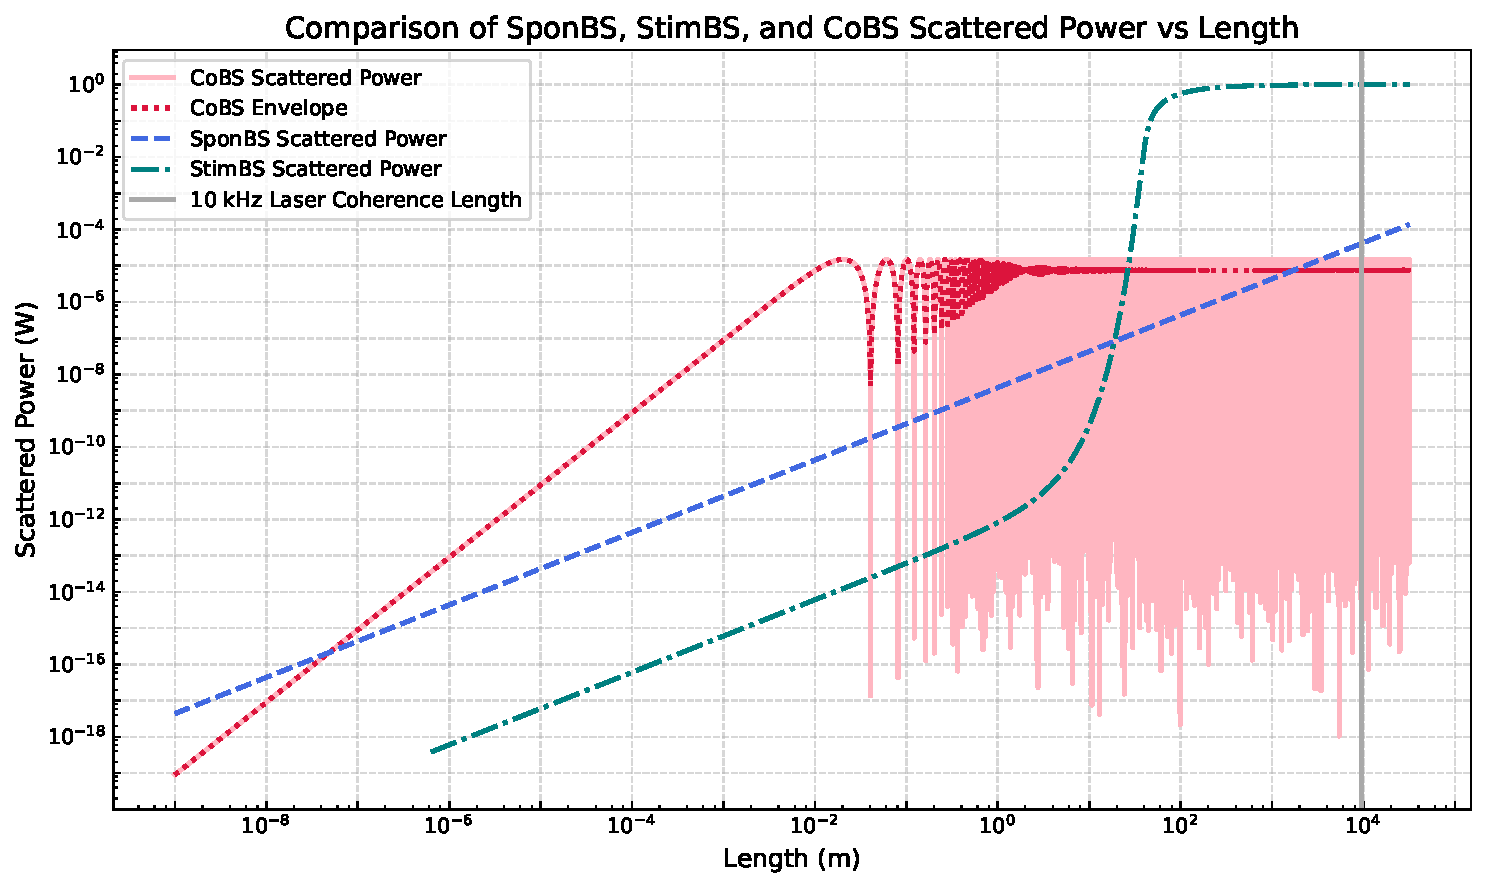
\includegraphics[width=\textwidth]{figs/4-CoBS/SponBSvsStimBSvsCoBS.pdf}
\caption{Comparison of scattered power from a spontaneous Brillouin scattering process and our coherently stimulated Brillouin spectrometer.}
\label{fig:SponBSvsStimBSvsCoBS}
\end{figure}

Figure~\ref{fig:SponBSvsStimBSvsCoBS} shows the advantage that our coherently stimulated Brillouin spectrometer offers compared to the traditional Brillouin processes for the example medium of UHNA3 fiber. For lengths up to about 50 meters and down to as low as 100 nanometers, the coherently stimulated process employed by our instrument offers superior scattered power, with the relative advantage peaking for a length just under 1 cm. At this length, the gain factor $G$ places the traditional process within the low-gain (spontaneous) regime, and thus the scattered power generated is only on the order of 10s of picoWatts. In contrast, the scattered power for the same system offered by our instrument is on the order of 10s of microWatts, exceeding that of the spontenous process by a factor of a million. This is, of course, the most ideal case for this system, however it can be seen from Figure~\ref{fig:SponBSvsStimBSvsCoBS} that the coherently stimulated process offers orders of magnitude more scattered power than either traditional process through a wide range of lengths.

\newpage

%--------------------------------------------------------------------%

\section{Observance of Fano-Resonant Asymmetries at Small Signals}
\label{Appendix:Fano}

In \textit{Fano-Resonant Asymmetries at Small Signals} (Section~\ref{Results:Fano-Resonant Asymmetries at Small Signals} in the main text), we discussed how Fano-type interference can distort Brillouin line shapes in situations where the resonant Brillouin amplitude becomes comparable to the background continuum. We focus here on two experiments (A and B) that reveal these Fano asymmetries especially clearly. Experiment~A is a measurement series using the same \SI{1}{\centi\meter} UHNA3 fiber referenced in the main discussion, for which the main text showed only the fitted amplitudes (Figure~\ref{fig:Phase-Match}). Here we show the full spectra, illustrating the emergence of asymmetries at lower amplitude conditions. Experiment~B is a distinct measurement involving a short (\(\sim\)\SI{1}{\milli\meter}) bulk liquid sample of carbon disulfide (\ce{CS2}) that we briefly mentioned in Section~\ref{Results:Fano-Resonant Asymmetries at Small Signals} but did not detail. This experiment was performed specifically to further probe the unexpected Fano-like distortions observed in Experiment~A. In each case, we outline the experimental setup, present the spectra, and highlight the appearance of Fano resonances. These observations corroborate the theoretical discussion of Fano line shapes (Section~\ref{Results:Fano-Resonant Asymmetries at Small Signals}) and provide insight into when and why they are most prominent.

\subsection{Experiment A: Extended \SI{1}{\centi\meter} UHNA3 Fiber Spectra}
\label{Appendix:Fano:Experiment A}

In Section~\ref{Results} of the main text, we introduced a phase-matching experiment on \SI{1}{\centi\meter} of UHNA3 fiber in which the pump--probe detuning was varied from \SI{5}{\giga\hertz} to \SI{42}{\giga\hertz} in \SI{0.5}{\giga\hertz} increments. There, we reported only the resulting peak amplitudes, showing how they follow a \(\mathrm{sinc^{2}}\) dependence on detuning (Figure~\ref{fig:Phase-Match} in the main text). However, each measurement in that scan also yields a full Brillouin spectrum—75 in total. Here, we present all 75 spectra to illustrate how the line shape transitions from nearly Lorentzian (when the Brillouin peak amplitude greatly exceeds the background continuum) to distinctly Fano-like (when the two amplitudes are comparable). We used the same setup and procedure described in \textit{Phase Matching Characterization} in Section~\ref{Results} of the main text. As the pump-probe detuning increases, the phase-matching term \(\mathrm{sinc^{2}(\Delta kL/2)}\) oscillates through peaks and troughs, causing the Brillouin peak amplitude to rise and fall. When the amplitude is sufficiently large, the Brillouin mode dominates the continuum and the spectrum appears nearly Lorentzian; when it drops to the order of the background amplitude, strong interference skews the line shape into a Fano-like profile.

Figure~\ref{fig:Joy Division UHNA3} highlights the progressive shift from Lorentzian to asymmetric line shapes. Near \SI{5}{\giga\hertz} detuning (top spectra), the resonant amplitude is large relative to the background, giving a classic Lorentzian peak (\(|q| \to \infty\)) at the resonance frequency (\(\sim\)\SI{9.17}{\giga\hertz}). By contrast, at detunings between \(\sim\)15-\SI{20}{\giga\hertz}, where the \(\mathrm{sinc^{2}}\) factor is near a local minimum, the peak amplitude falls to roughly the same level as the continuum, and Fano interference is observed. Interestingly, as the detuning is increased further, and the amplitude rises again on a subsequent “lobe” of the \(\mathrm{sinc^{2}}\) function, the spectra partly recover a Lorentzian shape. This cyclical behavior persists, with each local maximum yielding a near-Lorentzian profile and each local minimum reintroducing a strong Fano distortion. These observations confirm the relationship between Brillouin peak amplitude and continuum interference described in \textit{Fano-Resonant Asymmetries at Small Signals} in Section~\ref{Results}. When the Brillouin amplitude significantly exceeds the background, the discrete phonon resonance dominates, resulting in little or no asymmetry (\(|q| \to \infty\)). Once the two amplitudes become comparable, Fano interference skews the line shape, shifting the apparent peak frequency slightly and altering the slope on either side of the resonance. Analyzing selected spectra with both Lorentzian and Fano fits indicates that ignoring these distortions can lead to up to a 5–10\% misestimation of peak amplitude in the “trough” (low-amplitude) sets. This underscores the importance of employing a Fano model in small-signal measurements where the Brillouin peak may not tower over the background. A comparative analysis of a Lorentzian vs. Fano fit function applied to highly assymetric spectra is explored in the following section, for data gathered from Experiment~B.

\begin{figure}[ht]
\centering
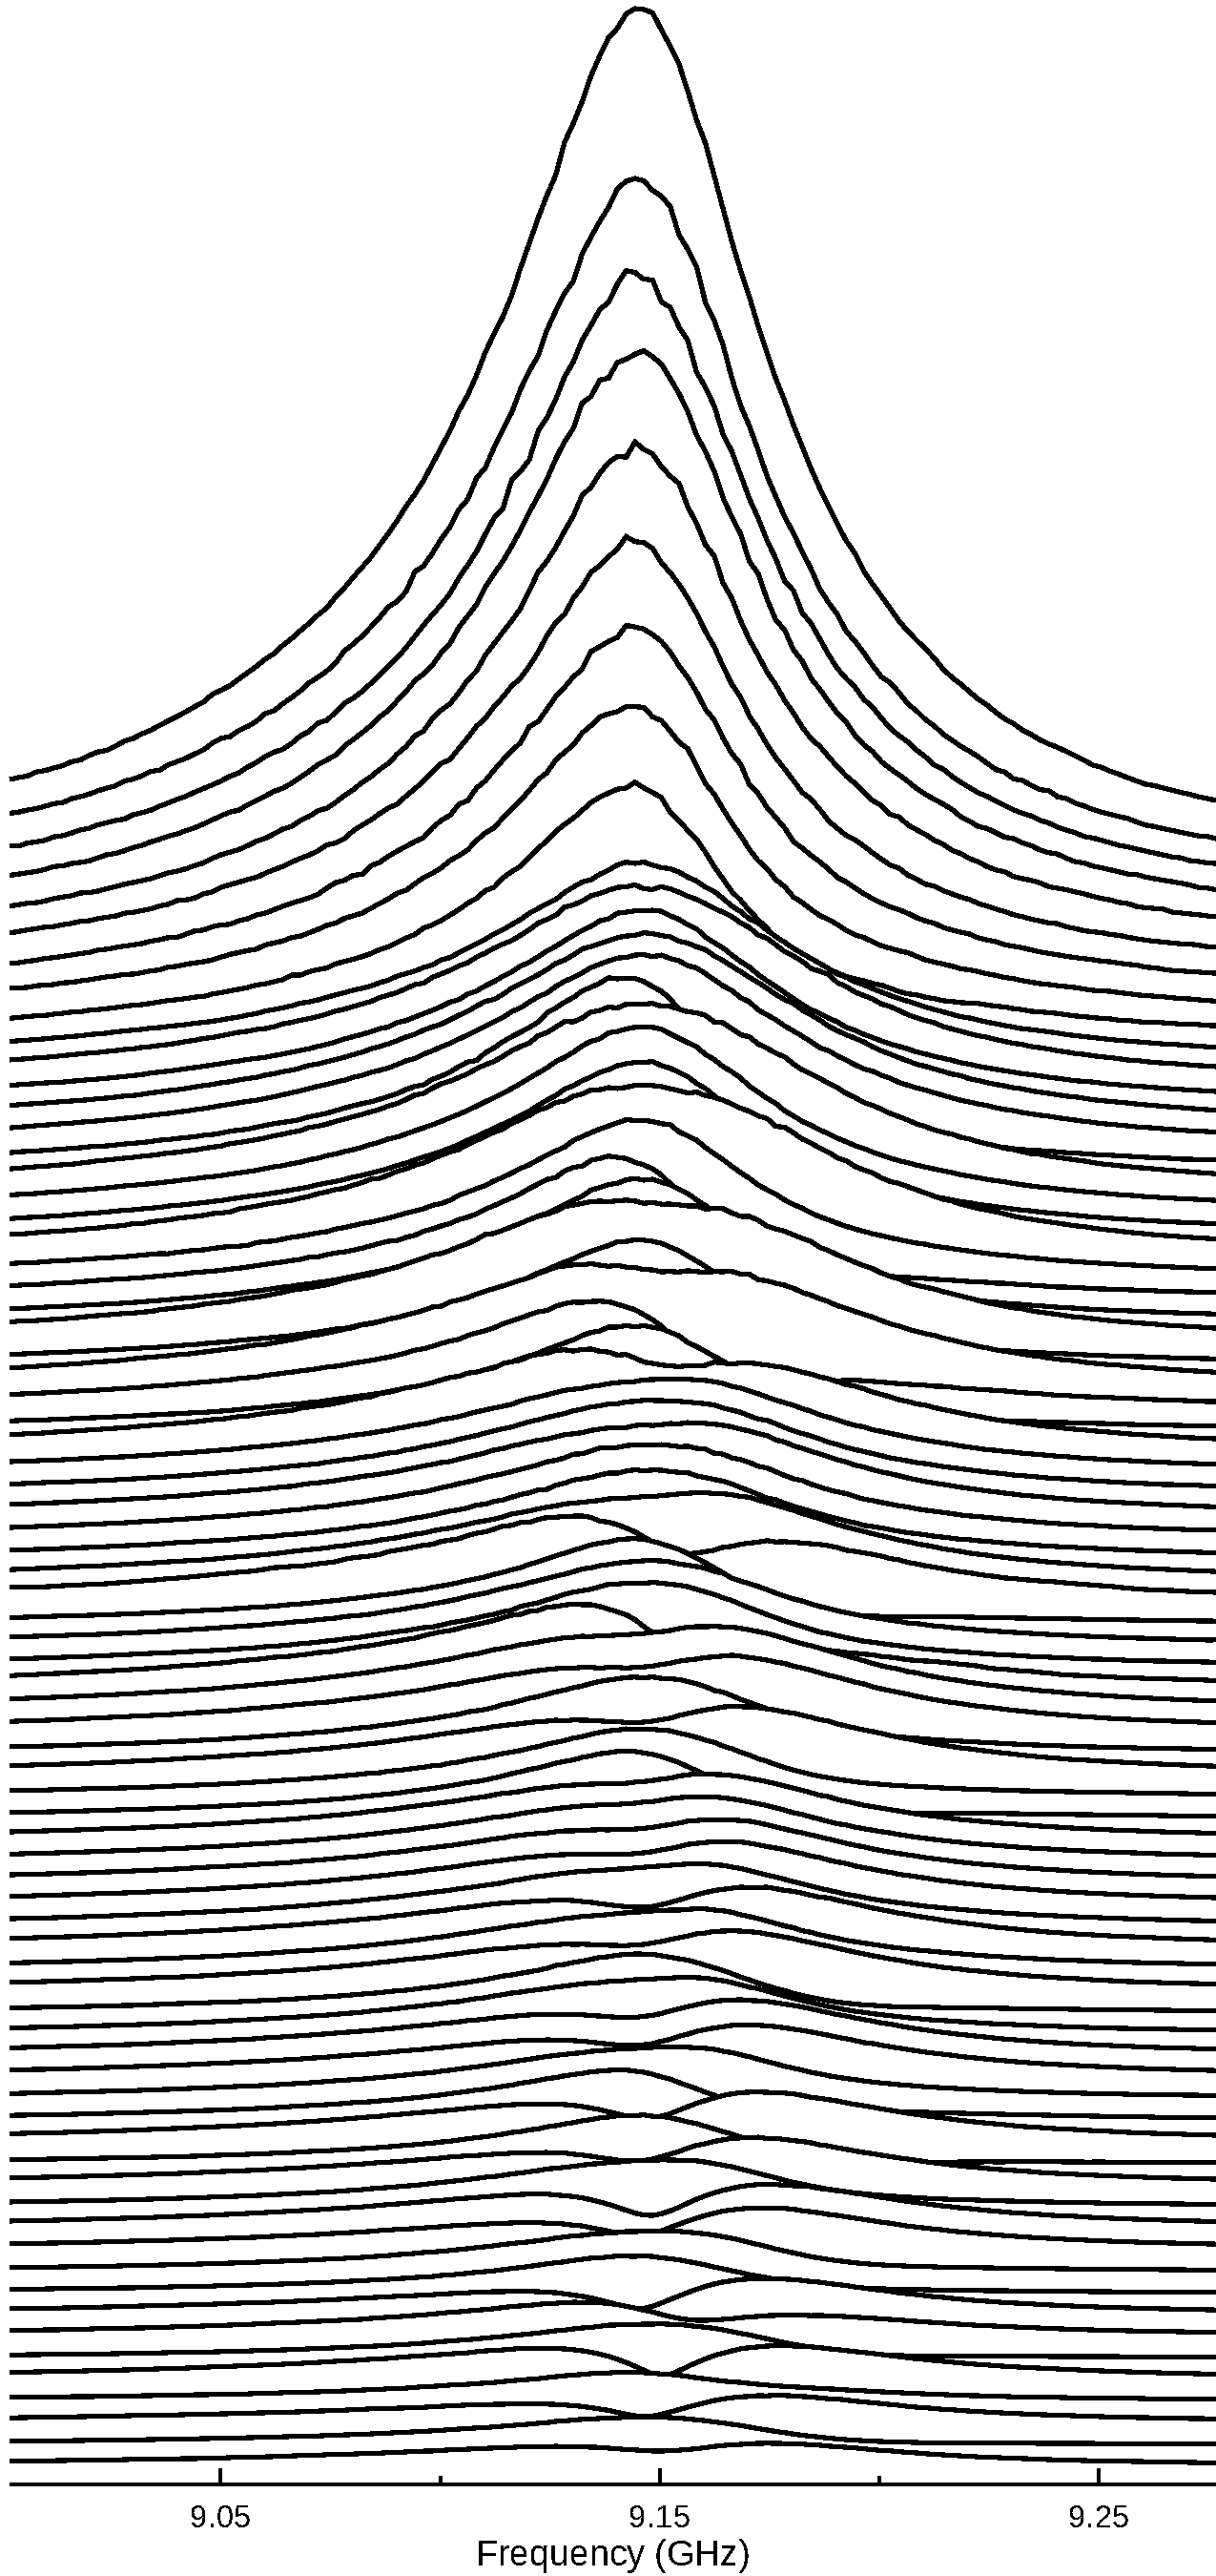
\includegraphics[height=0.90\textheight]{figs/4-CoBS/JoyDivisionCoBSUHNA3.pdf}
\caption{All measured Brillouin spectra for \SI{1}{\centi\meter}~UHNA3 at detuning steps of \SI{0.5}{\giga\hertz} from \SI{5}{\giga\hertz} (top spectrum) to \SI{42}{\giga\hertz} (bottom spectrum). Each trace is offset for clarity. The resulting asymmetries highlight the characteristic Fano-resonant behavior under low signal conditions.}
\label{fig:Joy Division UHNA3}
\end{figure}

\FloatBarrier

\subsection{Experiment B: \SI{1}{\milli\meter} \texorpdfstring{\ce{CS2}}{CS2} Spectra and Fano Distortions}
\label{Appendix:Fano:Experiment B}

We now turn to measurements on a \SI{1}{\milli\meter}-thick cell of \ce{CS2} in a free-space geometry, complementing the \SI{1}{\centi\meter} UHNA3 fiber results (Experiment~A). Both experiments used comparable sub-Watt optical powers (on the order of \(\sim\)60–\SI{70}{\milli\watt} pump, \(\sim\)25–\SI{30}{\milli\watt} Stokes, and \(\sim\)40–\SI{50}{\milli\watt} probe). However, unlike Experiment~A, which probed a \SI{1}{\centi\meter} fiber with \SI{0.5}{\giga\hertz} detuning increments from \SI{5}{\giga\hertz} to \SI{42}{\giga\hertz}, here the detuning is stepped in \SI{0.25}{\giga\hertz} increments between \SI{10}{\giga\hertz} and \SI{14}{\giga\hertz}. Because the \ce{CS2} sample is an order of magnitude shorter (\SI{1}{\milli\meter} vs.\ \SI{1}{\centi\meter}), its phase-matching bandwidth (\(\mathrm{sinc}^{2}\) profile) is roughly ten times wider, making these \SI{0.25}{\giga\hertz} steps effectively twenty times finer than the \SI{0.5}{\giga\hertz} steps used in the fiber experiment. This reduced range of detunings within a broader \(\mathrm{sinc^2}\) profile produce measured peaks all of similar amplitude to one another, as opposed to the dynamic evolution of peaks in the \SI{1}{\centi\meter} UHNA3 fiber data.

Figure~\ref{fig:Joy Division CS2} shows all 17 spectra obtained at detuning increments of \SI{0.25}{\giga\hertz}, presented in order of increasing detuning from top spectrum to bottom spectrum. Each trace is offset vertically for clarity, with the topmost spectrum corresponding to \SI{10}{\giga\hertz} and the bottom spectrum corresponding to \SI{14}{\giga\hertz} detuning of the pump and the probe. A change in the detuning of the pump and probe via adjustment of the probe laser wavelength produces a change in phase of the resonant Brillouin signal. This changing resonant Brillouin phase relative to the background continuum produces spectra with different Fano-resonant distortions corresponding to specific values of the Fano parameter, \(q\), as discussed in \textit{Fano-Resonant Asymmetries at Small Signals} in the main text (Section~\ref{Results:Fano-Resonant Asymmetries at Small Signals}). Fano-resonant asymmetries are seen in nearly every spectrum of this liquid experiment, indicating that the background continuum is competing strongly with the Brillouin amplitude in all measurements.

The Brillouin amplitudes featured in this experiment are an order of magnitude lower compared to the highest amplitudes seen in Experiment~A. This is caused by the order of magnitude shorter sample length of \ce{CS2} (\SI{1}{\milli\meter}) as compared to the \SI{1}{\centi\meter} length of UHNA3 fiber used in Experiment~A. The \(\sim\)1000 times higher Brillouin gain offered by the \ce{CS2} (\SI{1.5}{\meter\per\giga\watt}) is discounted significantly by the \(\sim\)350 times larger effective area offered by the beam waist in the free-space optical setup compared to the core of UHNA3 fiber used in Experiment~A (\(\sim\)\SI{17}{\micro\meter} radius beam waist vs. \(\sim\)\SI{0.9}{\micro\meter} radius core of UHNA3). The effective Brillouin gain of the \ce{CS2} used in Experiment~B is thus a net \(\sim\)3 times greater than that of the UHNA3 fiber. From Equations~\ref{Eq:Theoretical Framework:Scattered Power} and \ref{Eq:Effective Brillouin Gain} in the main text, scattered power scales with the square of both the length and the effective Brillouin gain of the sample (\(P_{Sig} \propto L^{2}G_{B}^{2}\)). Cumulatively, this makes for an approximate order-of-magnitude signal reduction for similar optical powers and pump-probe detuning.

However, both experiments (A and B) feature a sweep through a range of pump-probe detunings, with Experiment~B featuring a step size effectively 25 times finer than that of Experiment~A. This further corroborates these two data sets, as the signal reduction from near-center peak to a side trough of the \(\mathrm{sinc^{2}}\) profile is also on the order of a 10 times reduction (Figure~\ref{fig:Phase-Match}). This places the signal amplitudes of the \ce{CS2} spectra from Experiment~B (all near \textit{peak-center} of its \(\mathrm{sinc^{2}}\) profile) on the same order as the signal amplitudes near the \textit{troughs} of the UHNA3 fiber spectra from Experiment~A. These spectra all share strong Fano asymmetries, indicating as they should that they all sit in a similar signal amplitude range: small enough that the background continuum competes but does not dominate over the signal.

\begin{figure}[ht]
  \centering
  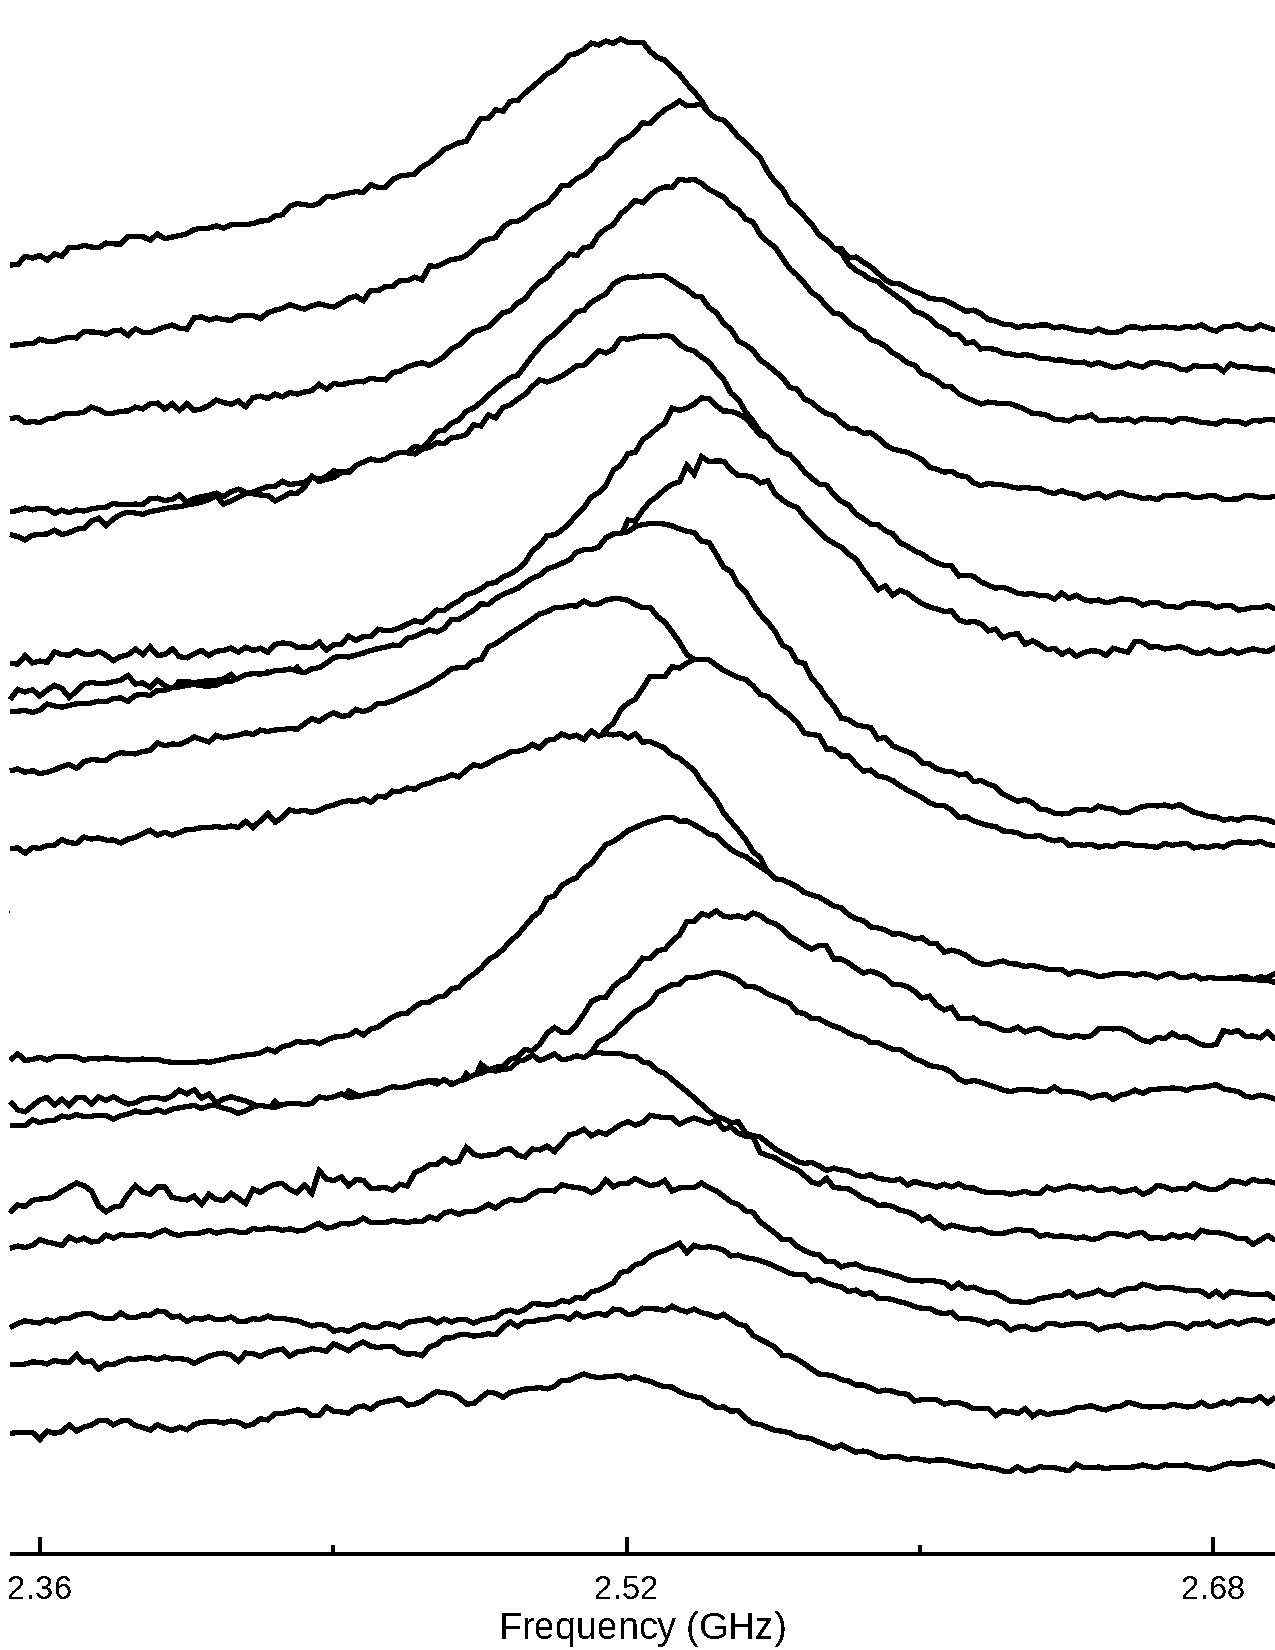
\includegraphics[width=0.7\textwidth]{figs/4-CoBS/JoyDivisionCoBSCS2.pdf}
  \caption{All measured Brillouin spectra for \SI{1}{\milli\meter}~\ce{CS2} at detuning steps of \SI{0.25}{\giga\hertz} from \SI{10}{\giga\hertz} (top spectrum) to \SI{14}{\giga\hertz} (bottom spectrum). Each trace is offset for clarity.}
  \label{fig:Joy Division CS2}
\end{figure}

\FloatBarrier

To illustrate the strong distinction in line-shape of a spectra resulting from a positive vs. negative \(q\) value, we focus on two particular detunings that yielded notably skewed line shapes: \SI{11}{\giga\hertz} and \SI{13}{\giga\hertz}. Figures~\ref{fig:CS2FanoCompare} and \ref{fig:CS2LorentzCompare} compare the spectra for these two detunings normalized relative to the slightly larger peak amplitude of the \SI{11}{\giga\hertz} spectra. The line-shape of the \SI{11}{\giga\hertz} spectrum exhibits a sharper rise on the higher-frequency side and a gentler roll-off on the lower-frequency side, indicative of \(q<0\), whereas that of the \SI{13}{\giga\hertz} spectrum is skewed oppositely, featuring a sharper low-frequency side and a softer high-frequency roll-off, suggesting \(q>0\). Figure~\ref{fig:CS2FanoCompare} shows these two spectra with uncertainty-weighted Fano function fits applied, with the corresponding reduced \(\chi^{2}\) values reported in the legend. The Fano fits yield reduced \(\chi^{2}\) values of 2.45 and 8.41 for the \SI{11}{\giga\hertz} and \SI{13}{\giga\hertz} spectra, respectively (reduced \(\chi^{2}\) values near unity indicate a good fit to the data). Figure~\ref{fig:CS2LorentzCompare} shows these same spectra with naïve Lorentz function fits applied and their corresponding reduced \(\chi^{2}\) evaluations of goodness-of-fit. These Lorentzian fits yield reduced \(\chi^{2}\) values of 39.45 and 146.5 for the \SI{11}{\giga\hertz} and \SI{13}{\giga\hertz} spectra, respectively, indicating that the Lorentzian function is a very poor fit to the data.. The poor fit of the Lorentzian function is due to its inherent symmetry, whereas the underlying data exhibit strongly asymmetric lineshapes. These results clearly demonstrate the superiority of the Fano model in capturing the asymmetry of small signals produced by the instrument due to Fano interference with the background continuum. This, in turn, emphasizes the importance of applying a Fano fit function when asymmetries arise to accurately extract valuable spectra parameters such as peak amplitude, center frequency, and linewidth from the data.

% Notably, in the negative-\(q\) case (\SI{11}{\giga\hertz}), the line’s peak amplitude appears slightly higher than what would be inferred from a Lorentzian fit—sometimes referred to as a “peak boost.” As discussed in \textit{Fano-Resonant Asymmetries at Small Signals} (Section~\ref{Results}), this can be beneficial for detecting weaker signals, provided the background is not too noisy, and in principle, one could choose a phase relationship that maximizes this constructive interference near resonance. Conversely, a positive-\(q\) scenario can suppress or broaden the peak on one side, which may be less desirable for line-shape analysis but could be exploited if one aims to shape the response profile in a particular way.

Notably, in the \(\SI{11}{\giga\hertz}\) case, our Fano fit reveals a local amplitude slightly higher than what the Lorentzian fit suggests, sometimes referred to as a “peak boost.” In essence, partial \emph{constructive} interference between the discrete Brillouin response and the broad continuum locally raises the amplitude, although it does not imply any net energy gain. As mentioned in \textit{Fano-Resonant Asymmetries at Small Signals} (Section~\ref{Results}), this effect can aid in detecting weak resonances if the background is not too noisy. One could, in principle, tune the phase relationship to maximize this interference near the resonance, possibly producing a sharper or taller peak for certain values of \(q\) than would be achieved without interference with the background. This Fano interference-tuning of the discrete mode relative to the background can be done dynamically via adjustment of the probe laser wavelength and, critically, can be adjusted independently from the phase-matching bandwidth tuning (pump-probe detuning). This is ability to dynamically adjust the discrete-continuum interference is an elegant and notable feature, as in typical systems this is adjusted via changes in physical geometry or material doping of the sample.\cite{ko2023full, gu2020fano, rieger2023fano}

\begin{figure}[ht]
  \centering
  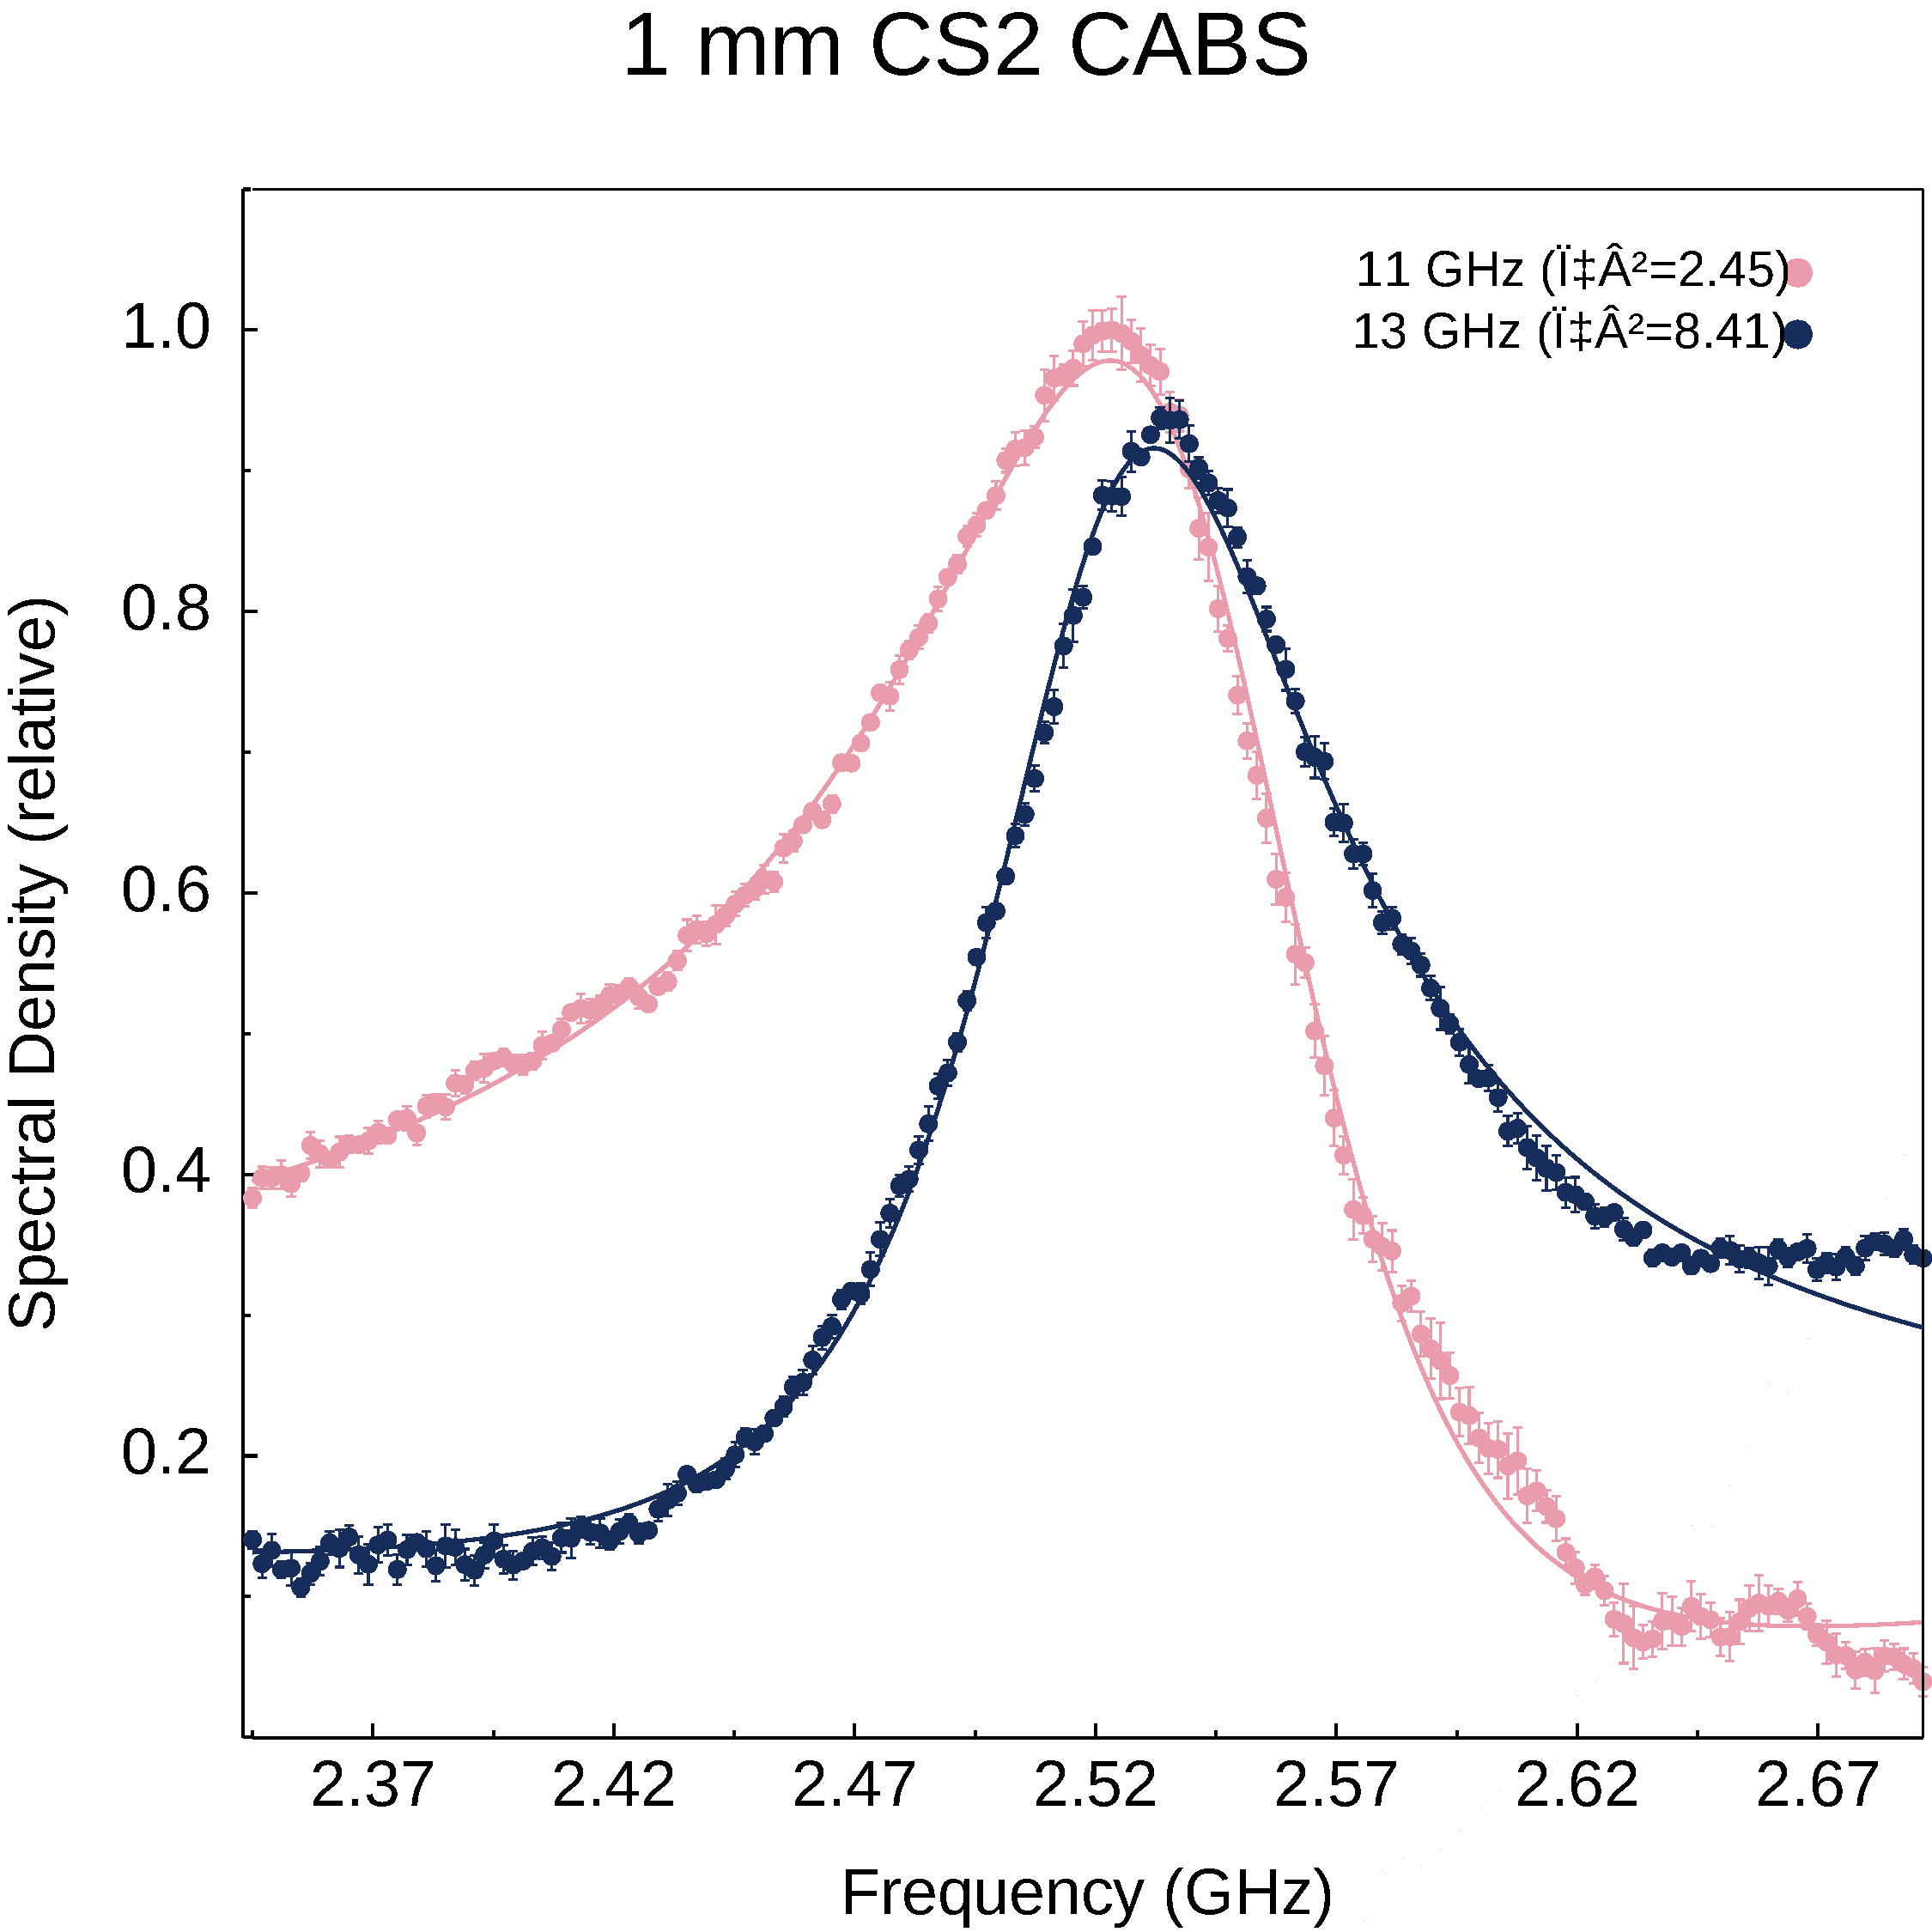
\includegraphics[width=\textwidth]{figs/4-CoBS/CS2FanoCompare.pdf}
  \caption{Comparison of representative spectra at \SI{11}{\giga\hertz} and \SI{13}{\giga\hertz}, showing the positive vs. negative \(q\) asymmetry in \SI{1}{\milli\meter} \ce{CS2}. A Fano function fit has been applied to each spectra, with \(\chi^{2}\) value for each fit listed in the plot legend.}
  \label{fig:CS2FanoCompare}
\end{figure}

\begin{figure}[ht]
  \centering
  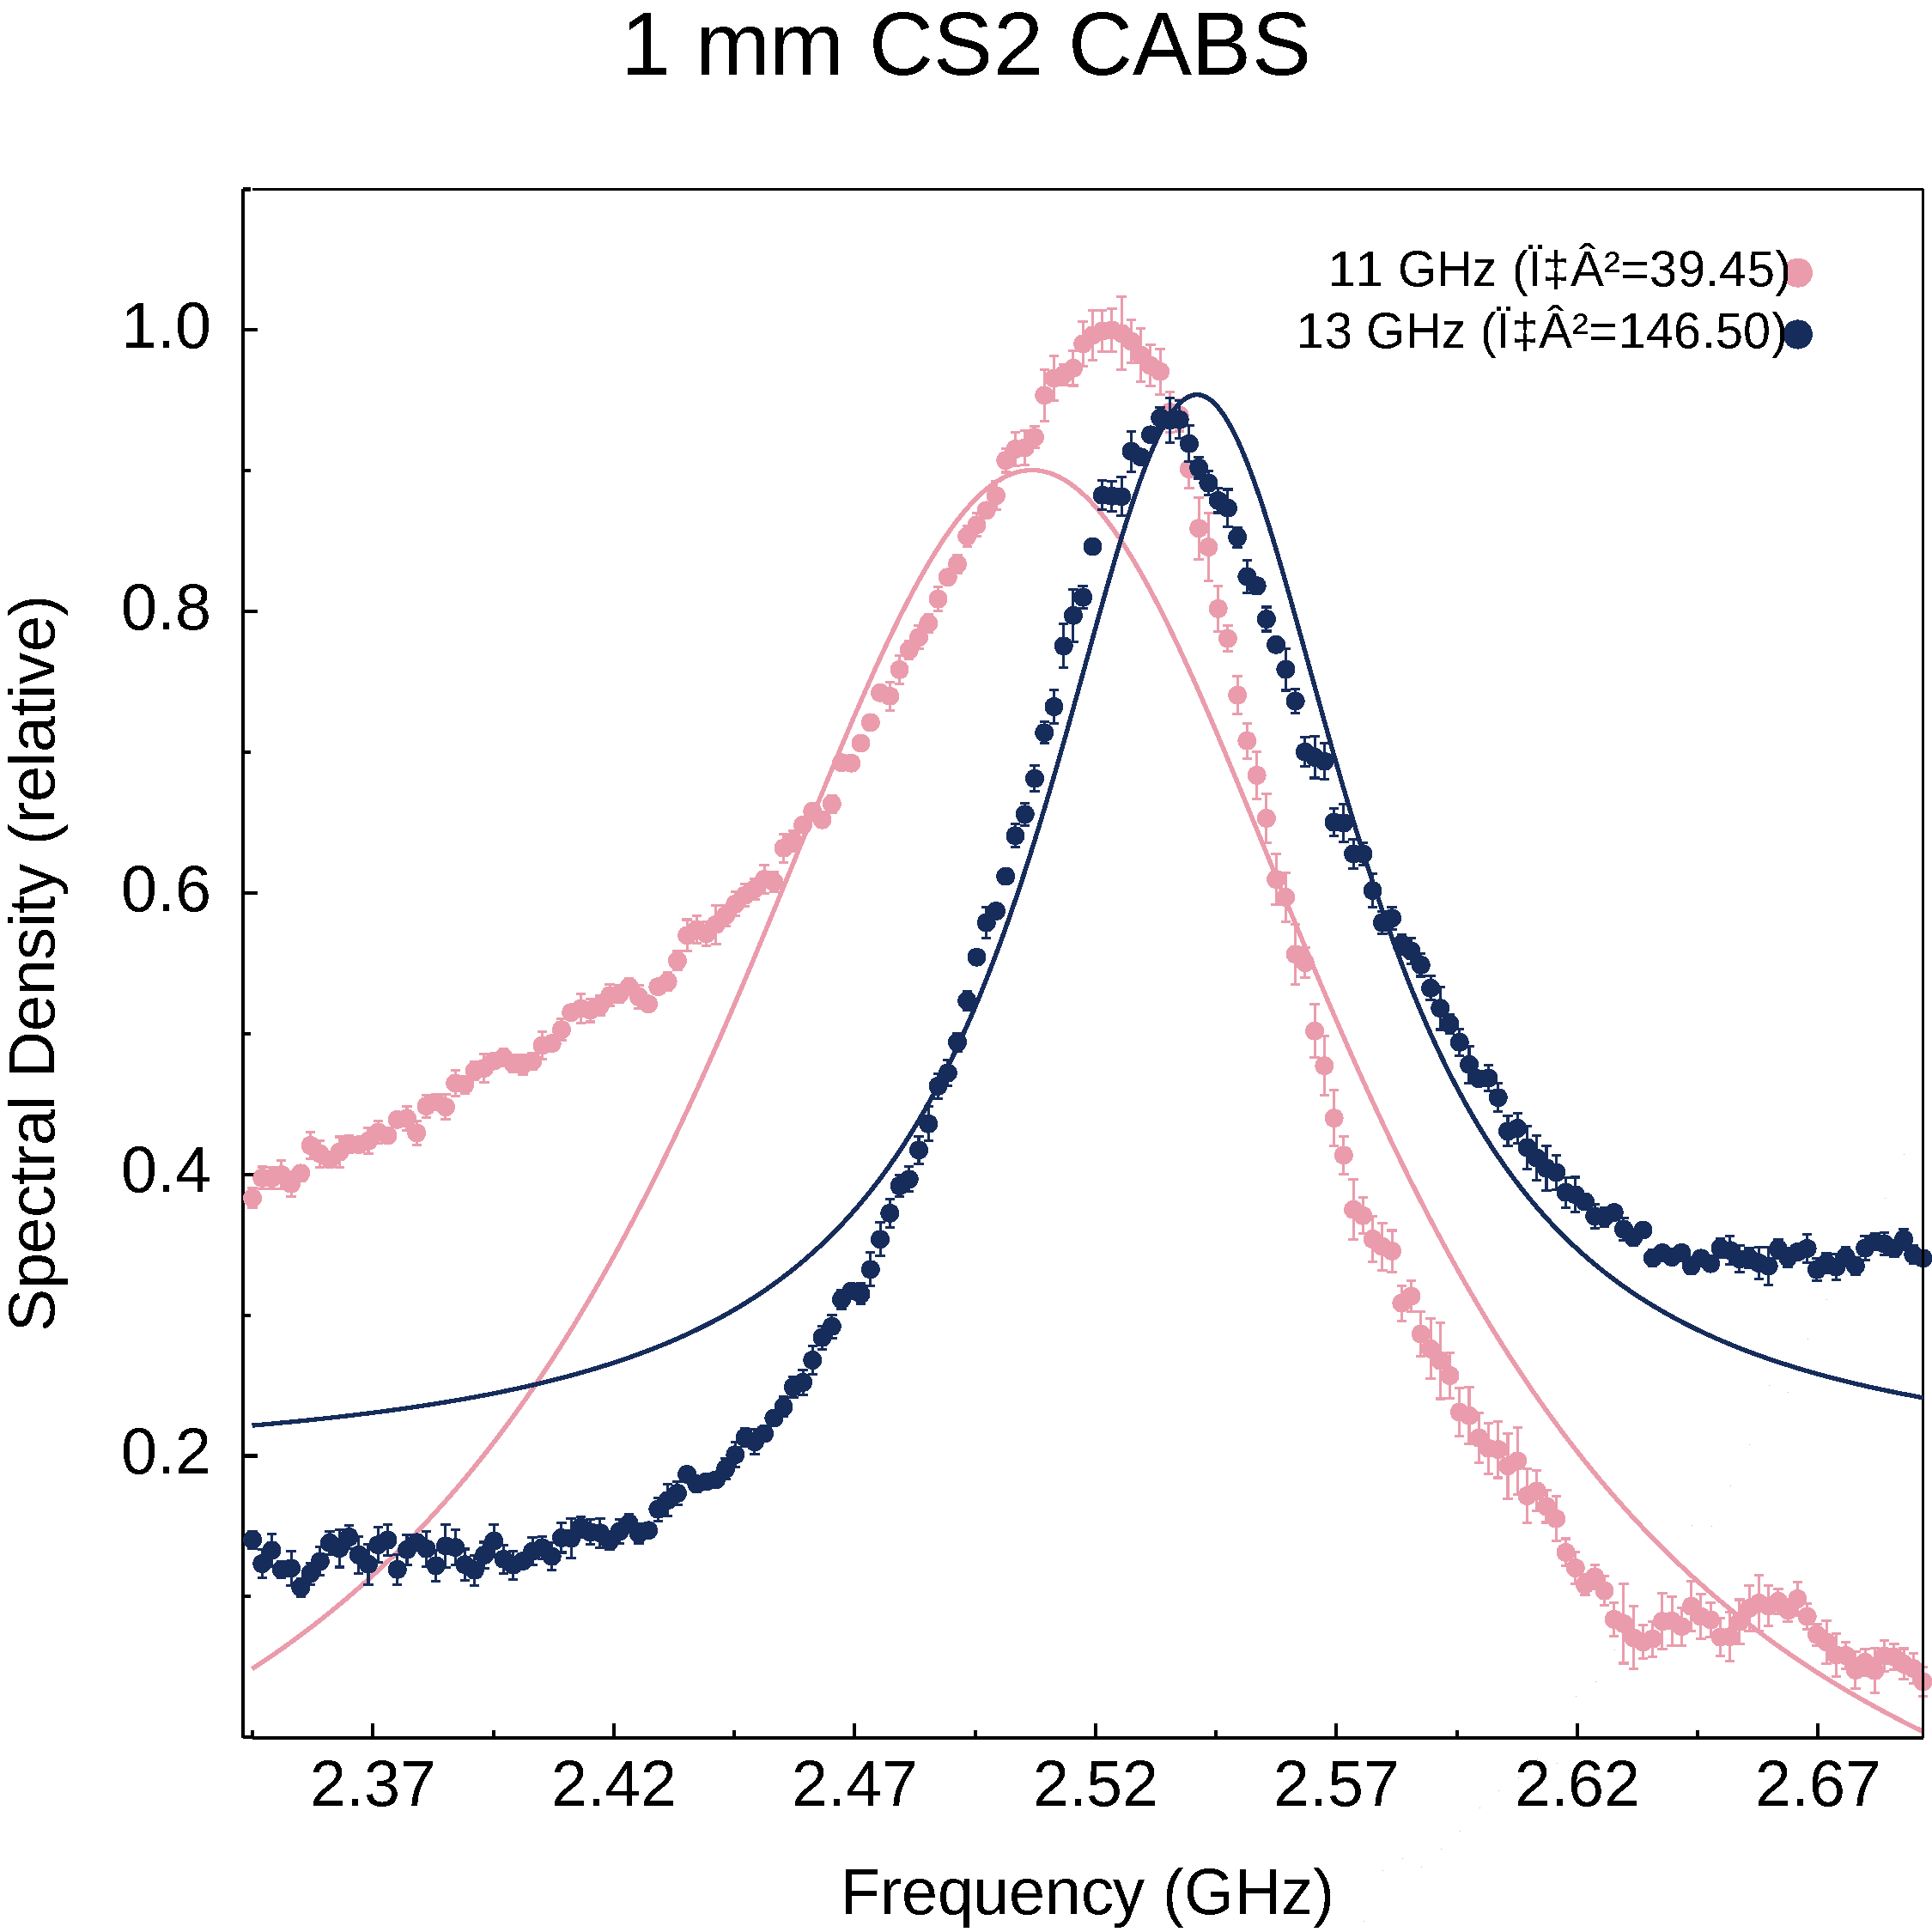
\includegraphics[width=\textwidth]{figs/4-CoBS/CS2LorentzCompare.pdf}
  \caption{Comparison of representative spectra at \SI{11}{\giga\hertz} and \SI{13}{\giga\hertz}, showing the positive vs.\ negative \(q\) asymmetry in \SI{1}{\milli\meter} \ce{CS2}. Here, a naïve Lorentz function fit has been applied to each spectra, with \(\chi^{2}\) value for each fit listed in the plot legend. These spectra show strong Fano-resonant asymmetry and thus the standard Lorentz function offers a poor fit for these spectra, quantified by the \(\chi^{2}\) evaluation metric for goodness of fit as compared to the same evaluation of the Fano function fit.}
  \label{fig:CS2LorentzCompare}
\end{figure}

\FloatBarrier

To better convey the cyclical evolution of the 75 measured UHNA3 spectra from Experiment~A, several animated GIFs have been generated. The following is a link to the GitHub repository which hosts these files, along with all raw data, measurement logs, and plots generated in support of this work (see See Appendix~\ref{appendix:CodeandDataAvailability}):

\hfill

\begin{center}
  \url{https://github.com/HamletTheHamster/Plotting-Data-in-Go}
\end{center}

\hfill

The reader will find several GIFs which step through each spectrum in ascending pump--probe detuning at various frame rates. Readers are encouraged to view them for an animated perspective on how the spectra evolve with increasing pump--probe detuning, with special attention to transitions between Lorentzian and Fano-distorted line shapes.

\newpage

%------------------------------------------------------------------------------%

\section{Mini Experiment: Equal Contribution of Pump, Stokes, and Probe}

Equation~\ref{Eq:Theoretical Framework:Scattered Power} gives the somewhat unintuitive result that the powers of the Pump, Stokes, and Probe waves contribute equally to the resulting scattered power of the Signal and invites verification with a miniexperiment. Initially, this experiment was motivated by a practical consideration: determination of whether the placement of a high power amplifier on any specific line of the setup (Pump, Stokes, or Probe) would offer any advantage over another.

To test this, we conducted a controlled experiment with a 1 mm carbon disulfide ($CS_{2}$) sample. For each measurement, one of the three source powers (Pump, Stokes, or Probe) was systematically reduced by 75\% while holding the others constant and ensuring consistent experimental conditions across trials. Table~\ref{tab:PSPr-Contribute-Equally} shows the respective powers for each source during the three measurements, along with the multiplicative total contribution of the three powers for each measurement towards the generation of scattered power of the Signal.

\begin{table}[ht]
  \centering
  \renewcommand{\arraystretch}{1.2}
  \begin{tabular}{|>{\centering\arraybackslash}m{2.5cm}|>{\centering\arraybackslash}m{2.5cm}|>{\centering\arraybackslash}m{2.5cm}|>{\centering\arraybackslash}m{2.5cm}|>{\centering\arraybackslash}m{2.5cm}|}
    \hline
    \shortstack{\rule{0pt}{2.5mm} \\ \textbf{Measurement} \\ \rule{0pt}{2.5mm}} &
    \shortstack{\textbf{Pump Power} \\ \textbf{(mW)}} &
    \shortstack{\textbf{Stokes Power} \\ \textbf{(mW)}} &
    \shortstack{\textbf{Probe Power} \\ \textbf{(mW)}} &
    \shortstack{\textbf{Total} \\ \textbf{(mW$^{3}$)}} \\
    \hline
    Pump Lower & 19.190 & 32.210 & 54.560 & 3.372 $\times 10^{4}$ \\
    Stokes Lower & 76.600 & 8.020 & 54.650 & 3.359 $\times 10^{4}$ \\
    Probe Lower & 76.600 & 32.530 & 13.480 & 3.359 $\times 10^{4}$ \\
    \hline
  \end{tabular}
    \caption{Power values for each source (Pump, Stokes, Probe) across the three measurements, with the multiplicative total power for each setup.}
    \label{tab:PSPr-Contribute-Equally}
\end{table}

Figure~\ref{fig:PSPr-Contribute-Equally} displays the average results from these three measurements, plotted with error bars representing one standard deviation of the mean. For increased certainty, Figure~\ref{fig:PSPr-Contribute-Equally-2sigma} presents the same data with error bars extended to two standard deviations, providing additional confidence in the reproducibility of the results. This experiment confirms that the scattered Signal power indeed depends equally on each of the three contributing wave powers, as expected from the theoretical framework. Consequently, boosting the power of any of the three sources affects the Signal power equally, allowing flexibility in pragmatic design across any of the three lines. Ultimately, this result reinforces the reliability of Equation~\ref{Eq:Theoretical Framework:Scattered Power} for predicting Signal power across a range of power distributions within practical settings.

\begin{figure}[ht]
  \centering
  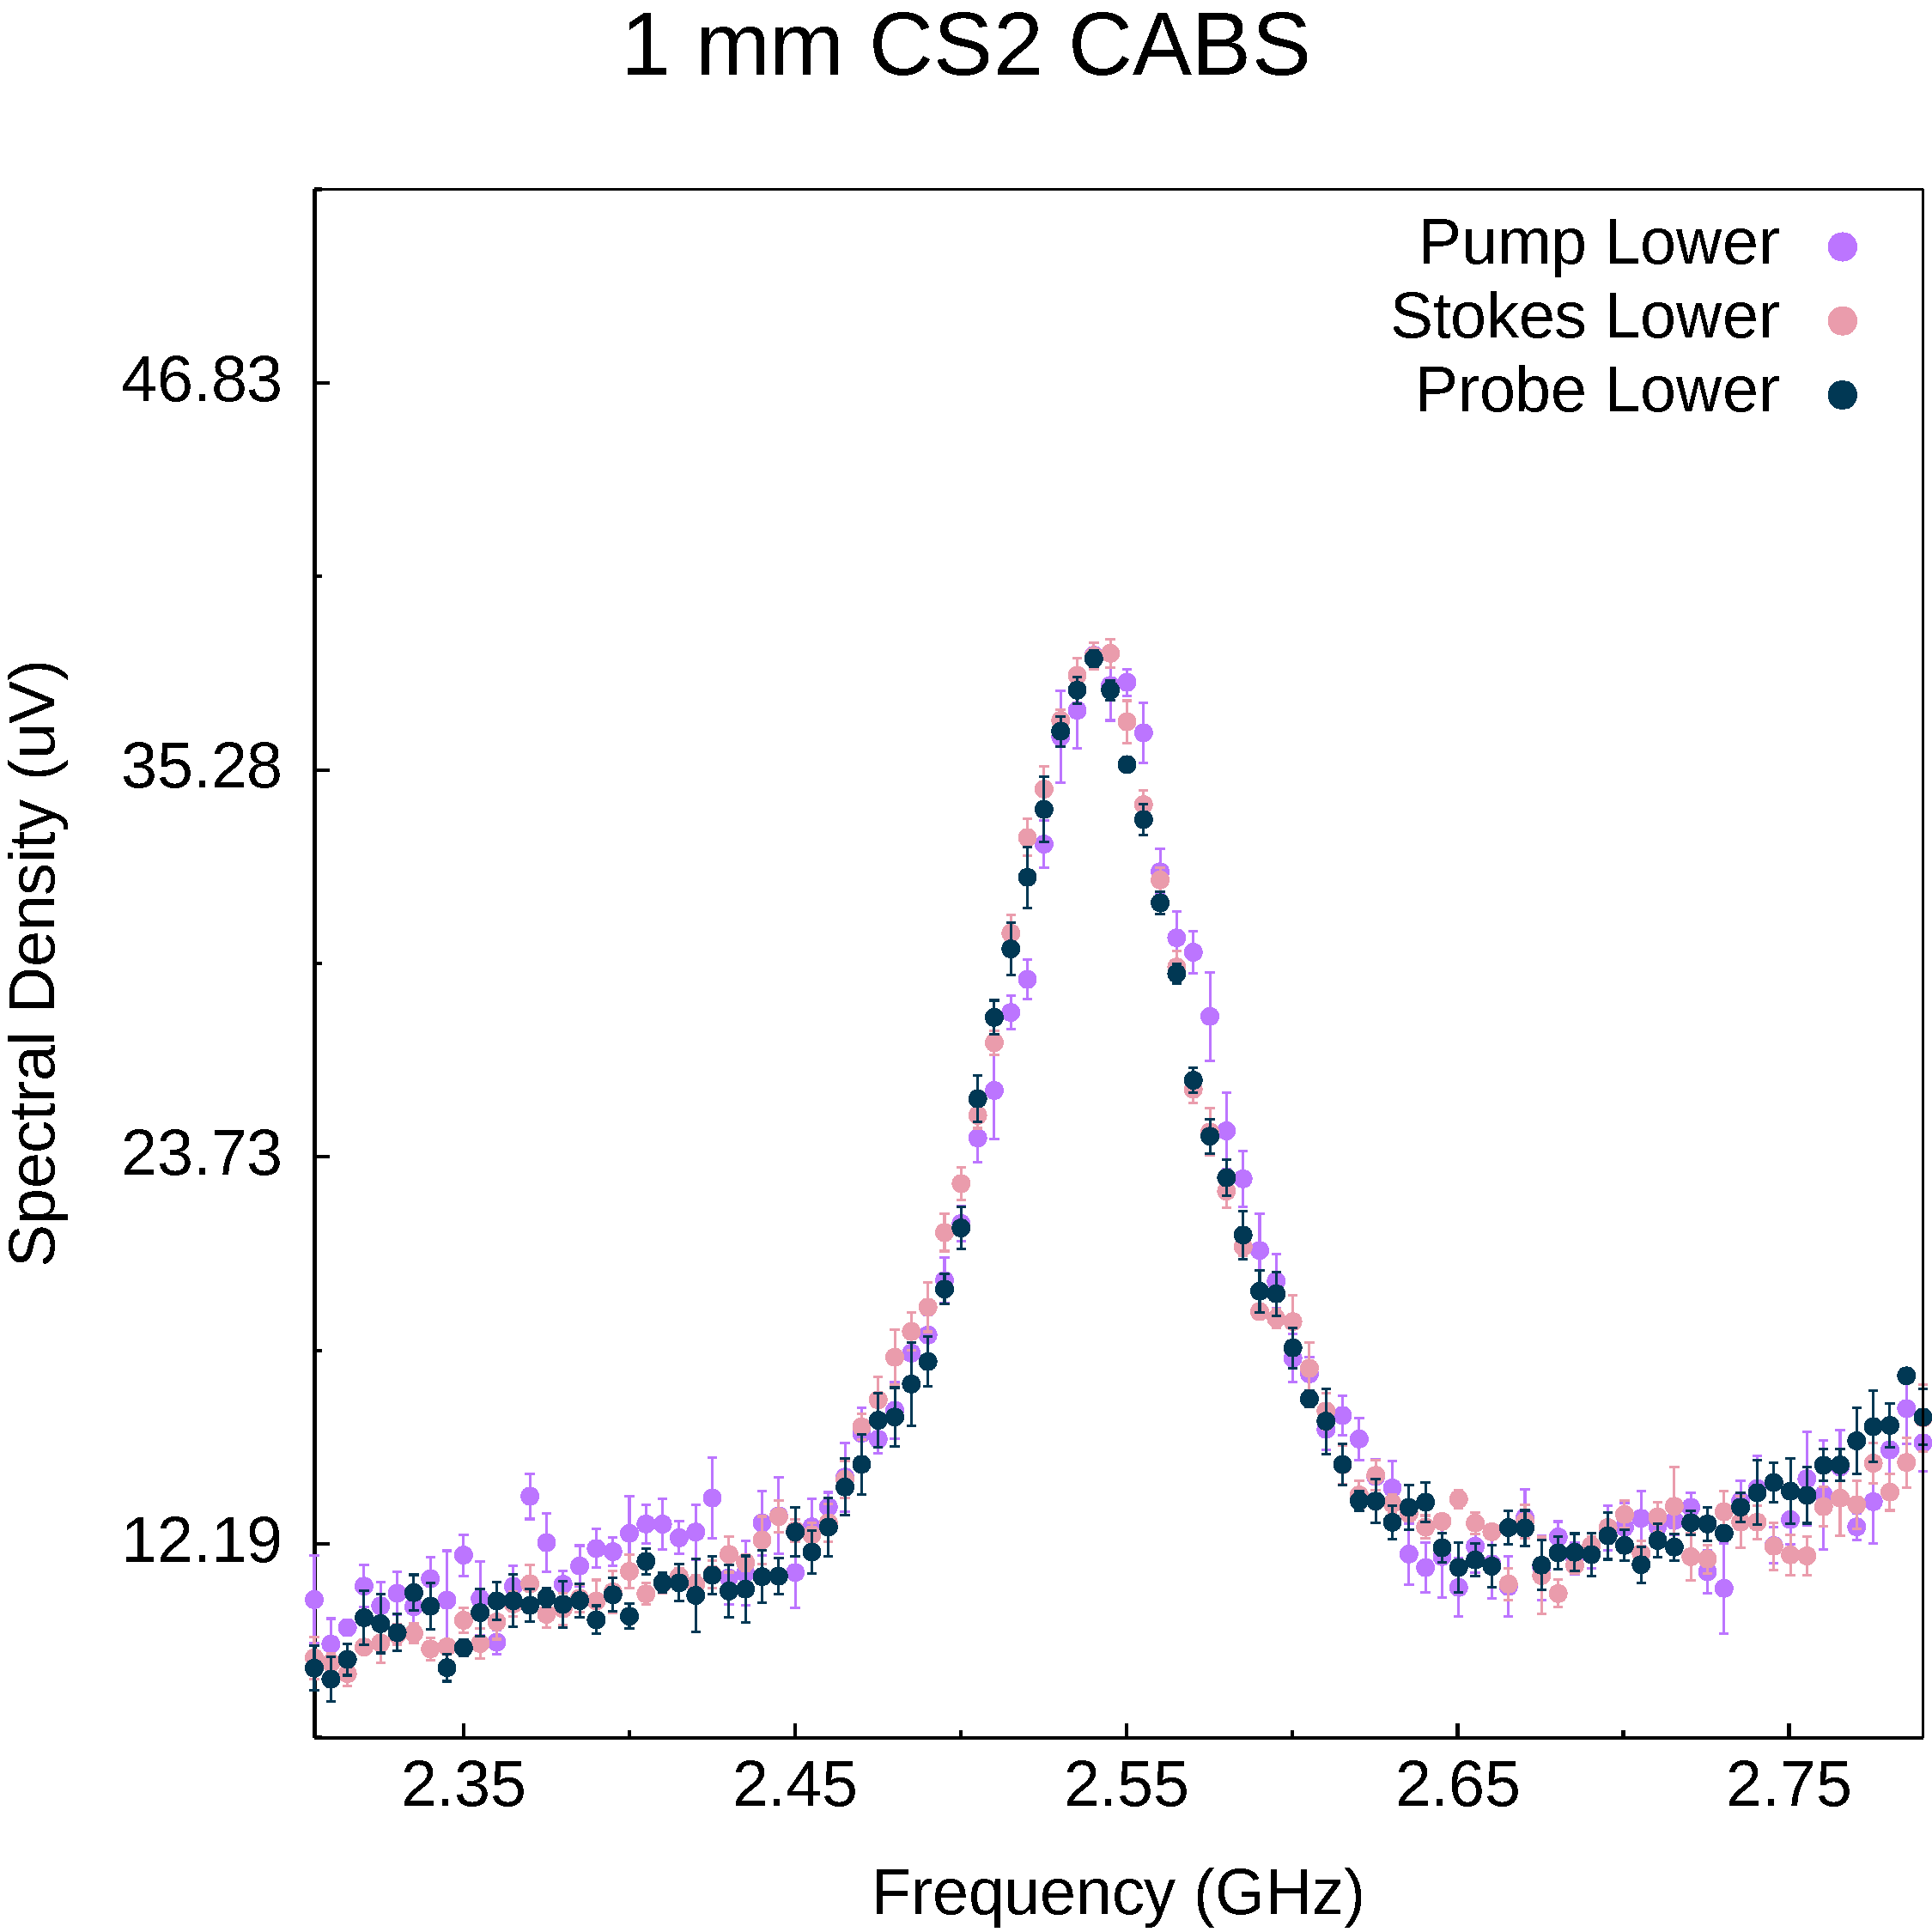
\includegraphics[width=\textwidth]{figs/4-CoBS/PSPr-Contribute-Equally.pdf}
  \caption{Signal power contributions with error bars representing one standard deviation of the mean for each measurement.}
  \label{fig:PSPr-Contribute-Equally}
\end{figure}

\begin{figure}[ht]
  \centering
  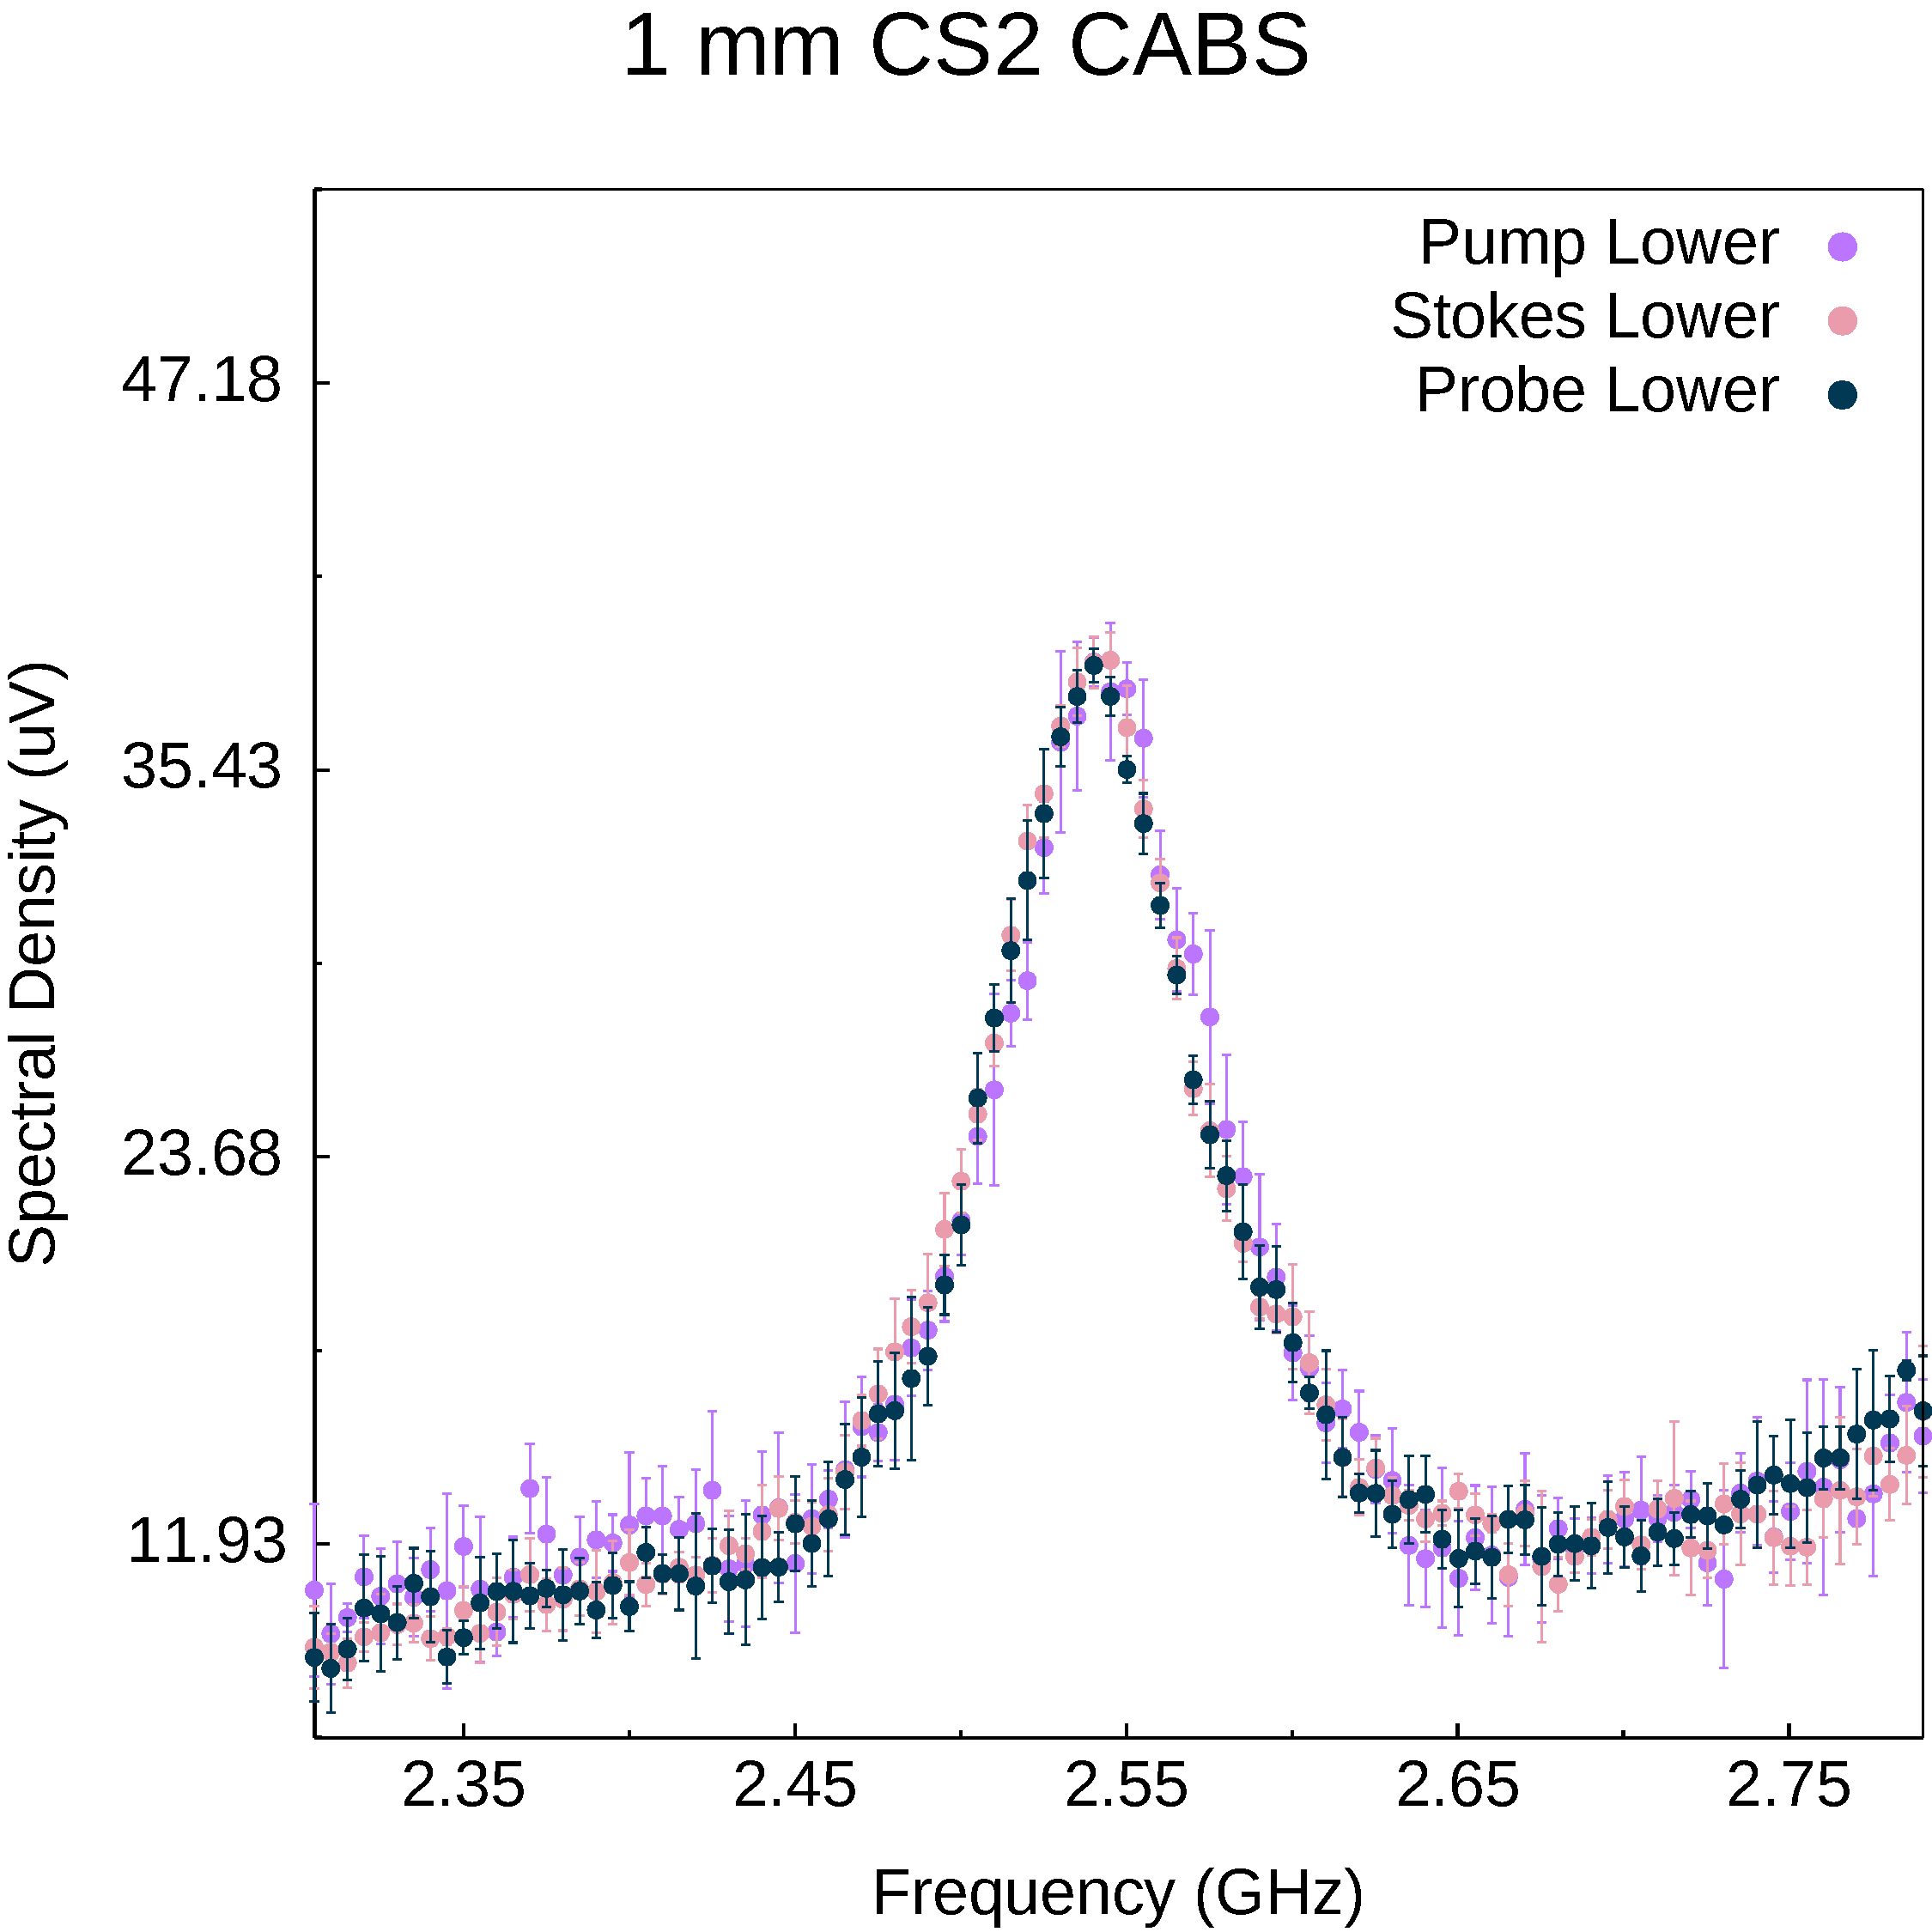
\includegraphics[width=\textwidth]{figs/4-CoBS/PSPr-Contribute-Equally-2sigma.pdf}
  \caption{Signal power contributions with error bars extended to two standard deviations of the mean for each measurement.}
  \label{fig:PSPr-Contribute-Equally-2sigma}
\end{figure}

\FloatBarrier

\newpage

\section{Data}


%\chapter{Supplementary Information for Chapter~\ref{ch:Raman}}
\label{appendix: Raman}
\acresetall

\section{Thin Film Fabrication via Physical Vapor Deposition}
\label{Raman:Appendix:sec:ThinFilmFabricationViaPVD}

Se adhesion layer
like rolling a ball down the outside of a cylinder
custom circuit to reduce thermal evaporation rate - course, fine

\begin{figure}[t]
  \centering
  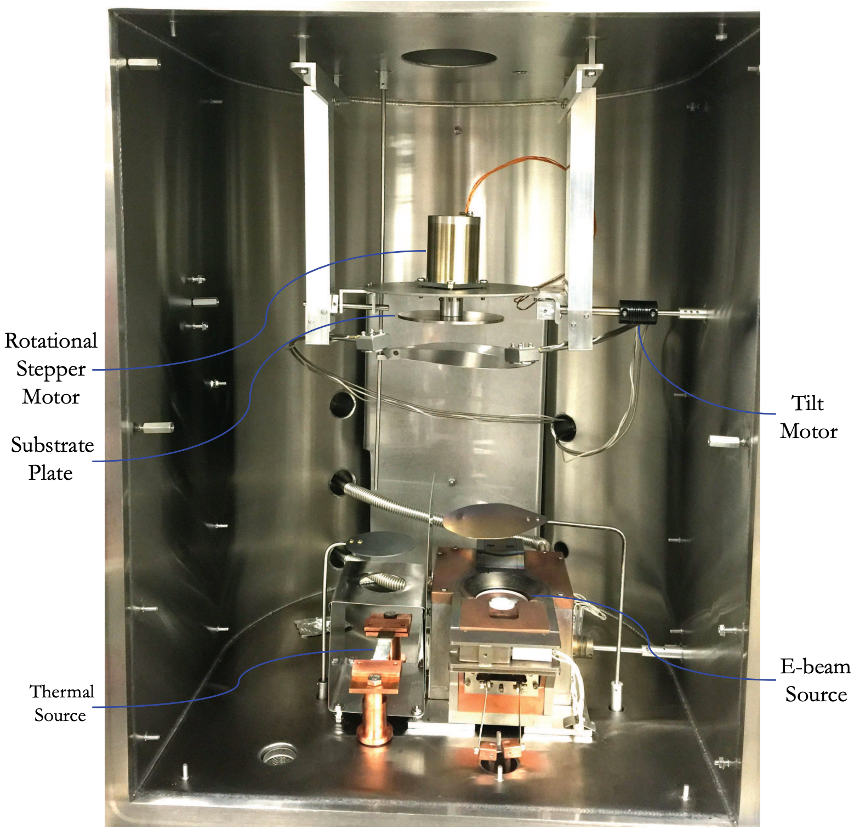
\includegraphics[width=\textwidth]{figs/4-Raman/DepositionChamber.png}
  \caption{Dr. John Gibbs Nanotechnology Laboratory \ac{PVD} chamber.}
  \label{fig:Raman:DepositionChamber}
\end{figure}

\begin{figure}[t]
  \centering
  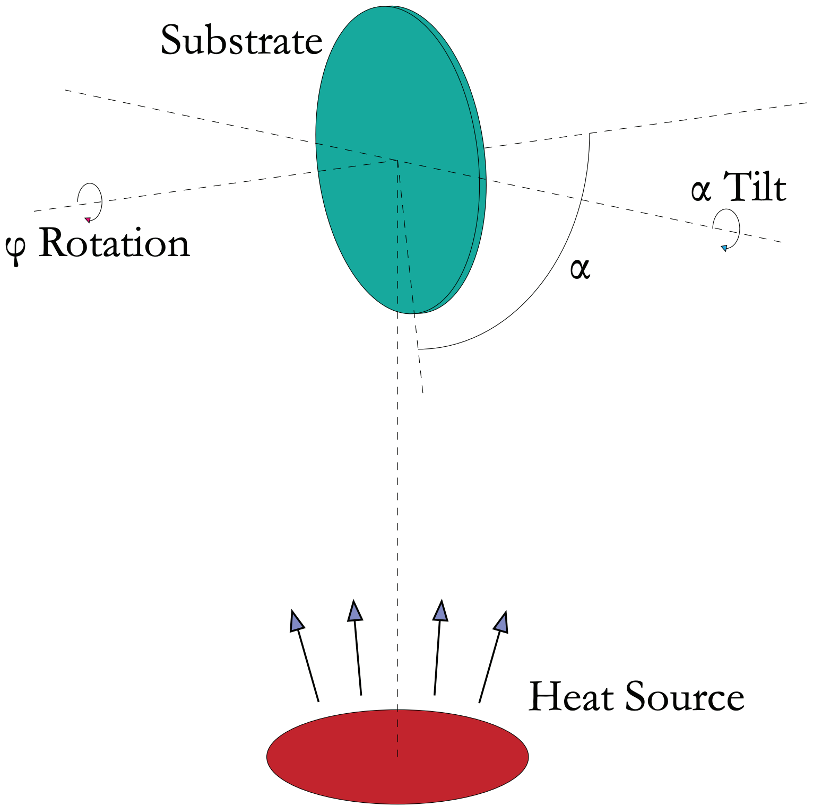
\includegraphics[width=.8\textwidth]{figs/4-Raman/GLAD.png}
  \caption{Diagram showing Glancing Angle Deposition (\acs{GLAD}). This technique offers the ability to fabricate complex nanostructures such as rods and helices via programatic control of deposition parameters and substrate degrees of freedom.}
  \label{fig:Raman:GLAD}
\end{figure}

\begin{figure}[t]
  \centering
  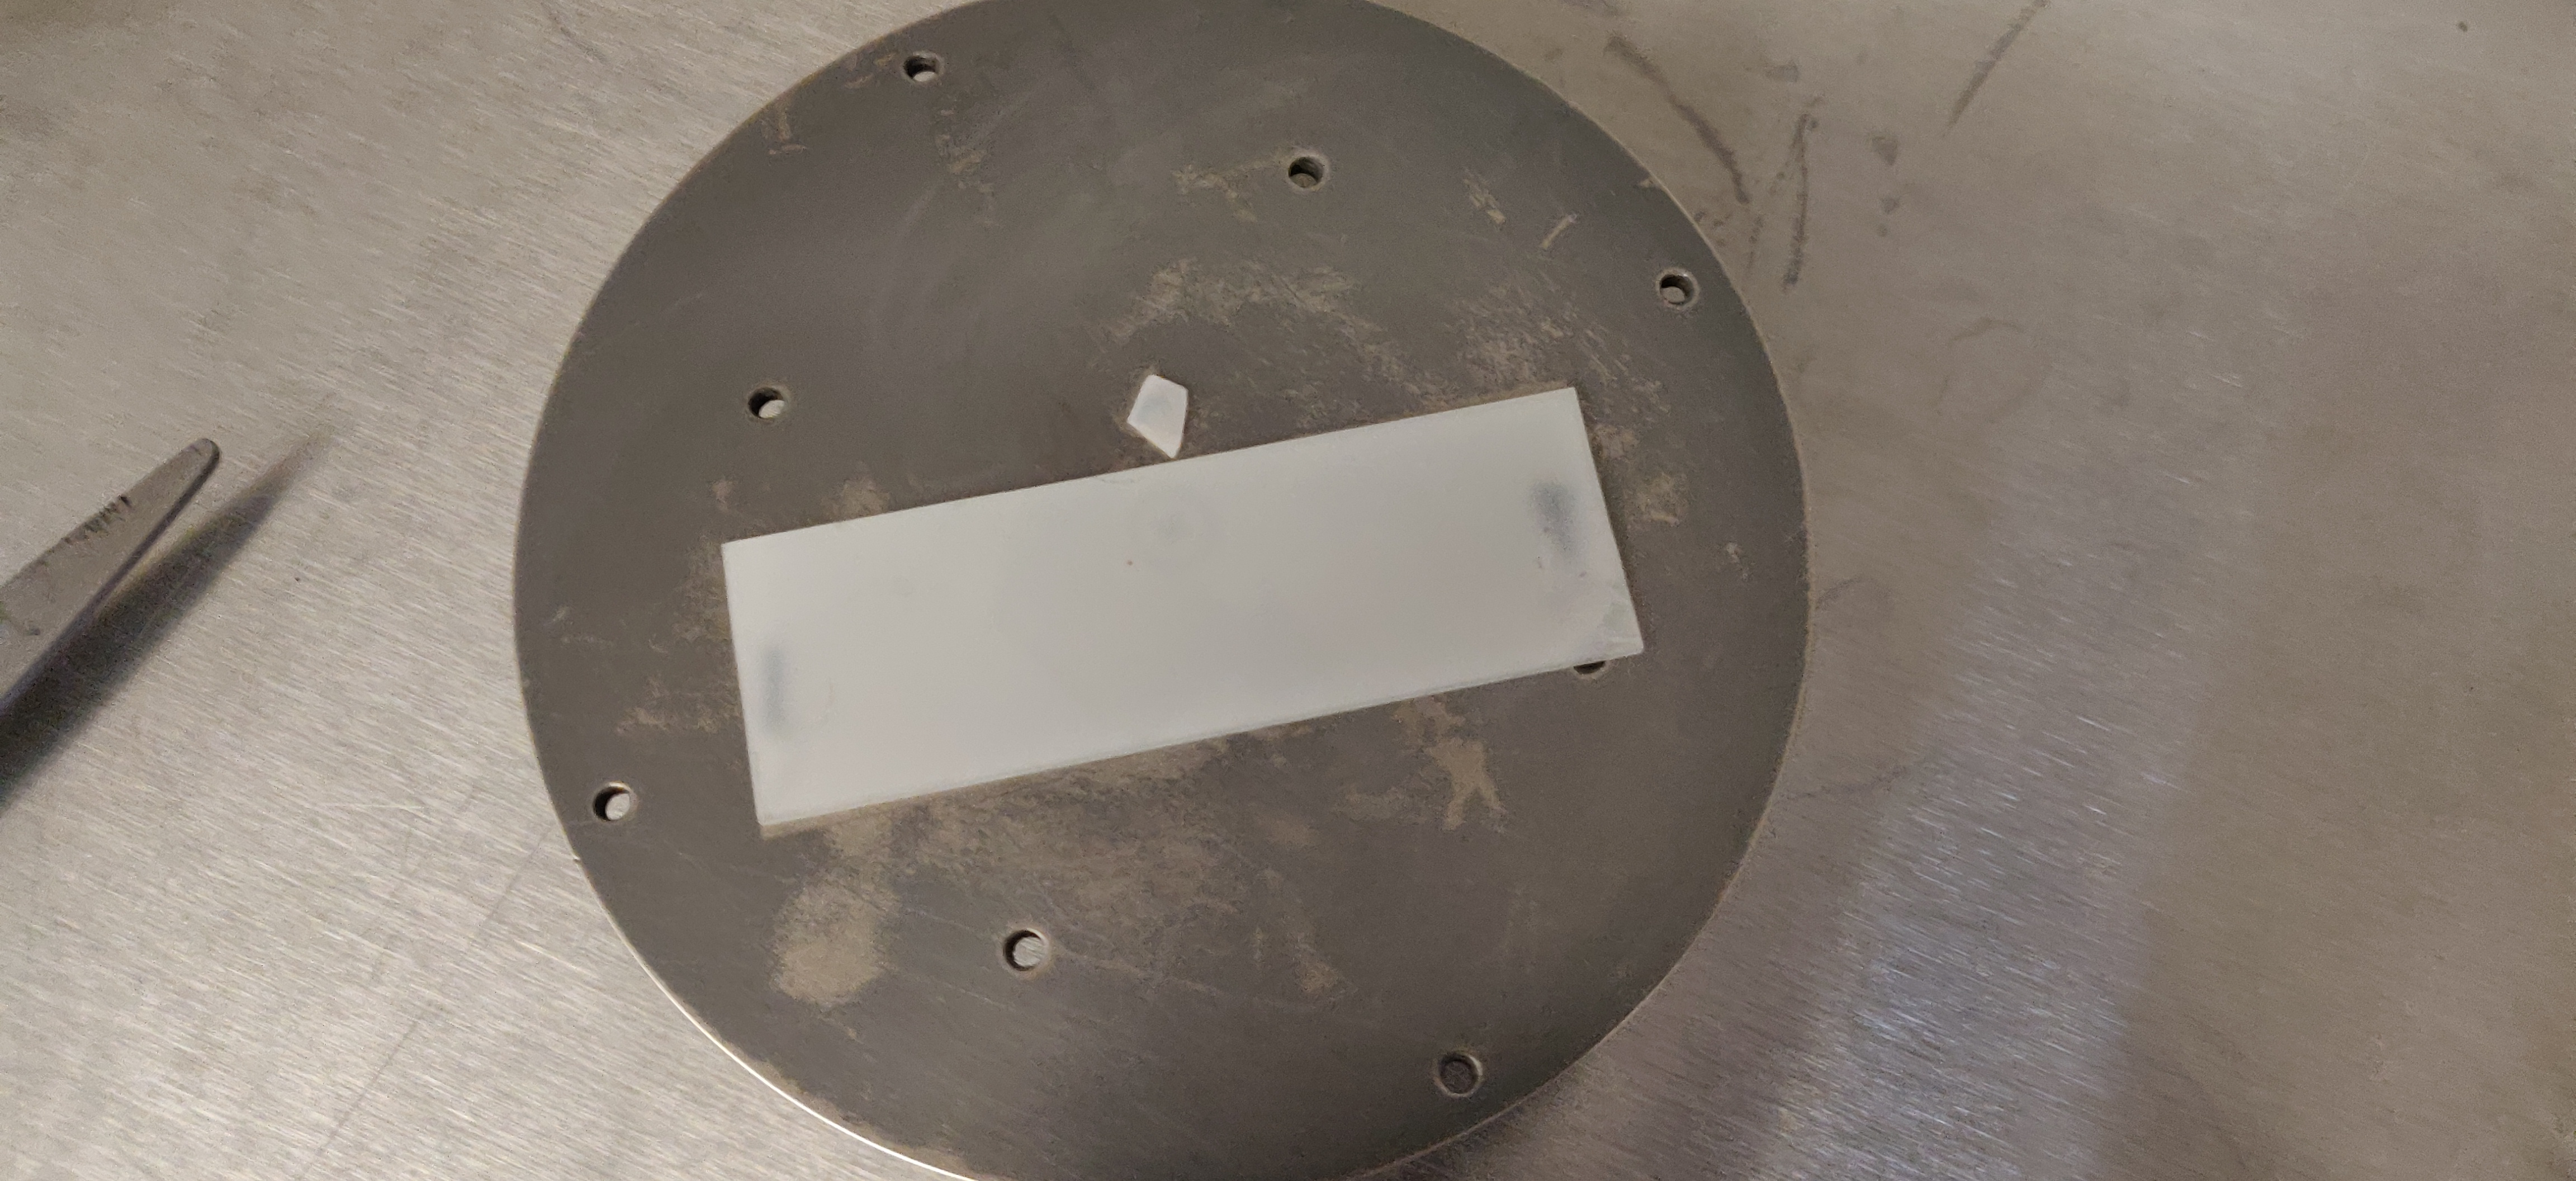
\includegraphics[width=\textwidth]{figs/4-Raman/slide-with-TeO2-film-on-substrate.jpeg}
  \caption{Photograph of \ce{TeO2} thin film deposited via \ac{PVD} onto glass slide substrate.}%was this deposited TeO2 or Te then annealed?
  \label{fig:Raman:TeO2onSubstrate}
\end{figure}

\begin{figure}[t]
  \centering
  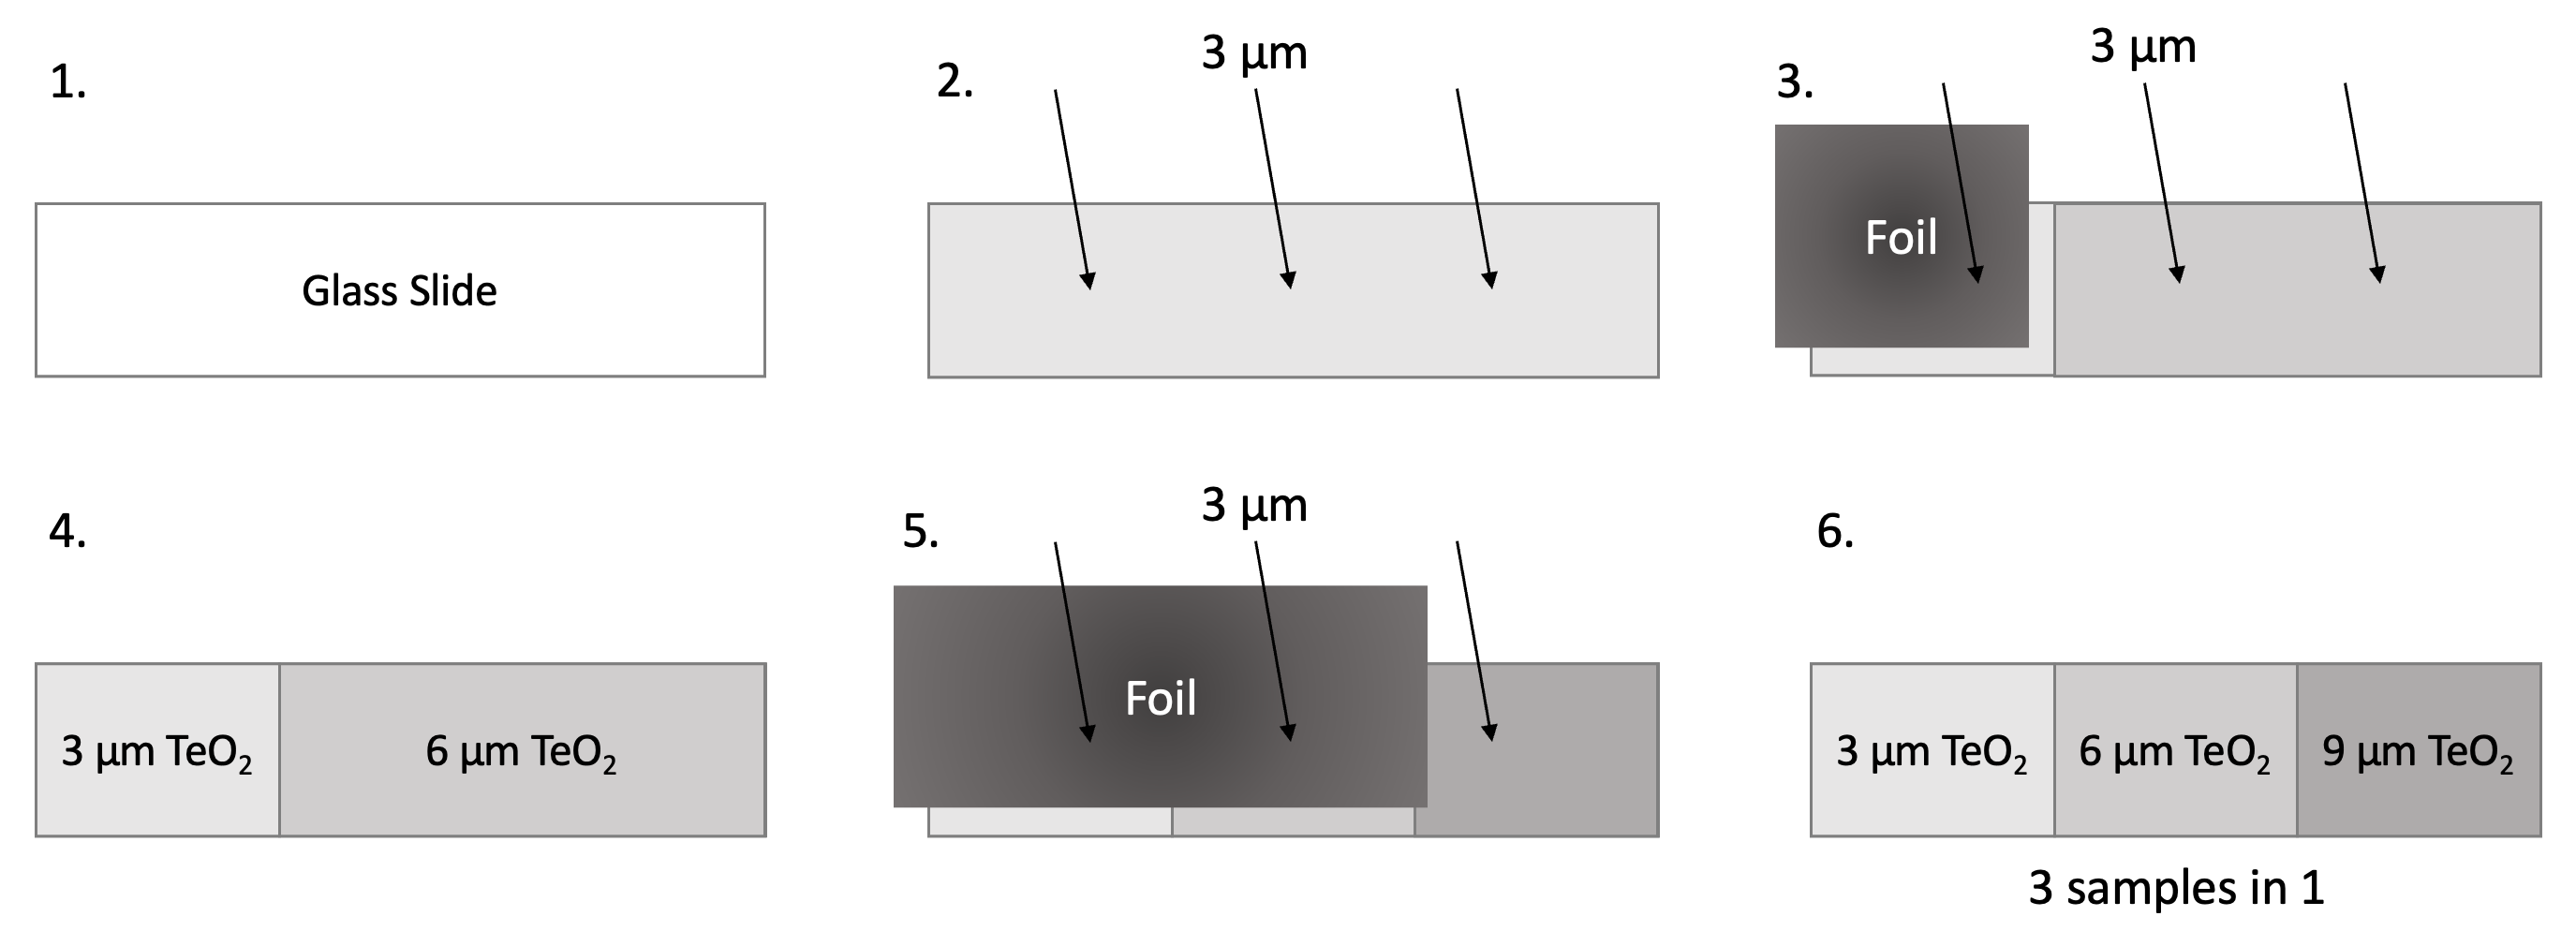
\includegraphics[width=\textwidth]{figs/4-Raman/3TeO2SamplesIn1.png}
  \caption{Diagram showing the multi-deposition process for fabricating \ce{Te} thin films of three thicknesses on one glass slide sample using \ac{PVD}.}
  \label{fig:Raman:3in1}
\end{figure}

\begin{figure}[t]
    \centering
    \begin{subfigure}[b]{0.49\textwidth}
        \centering
        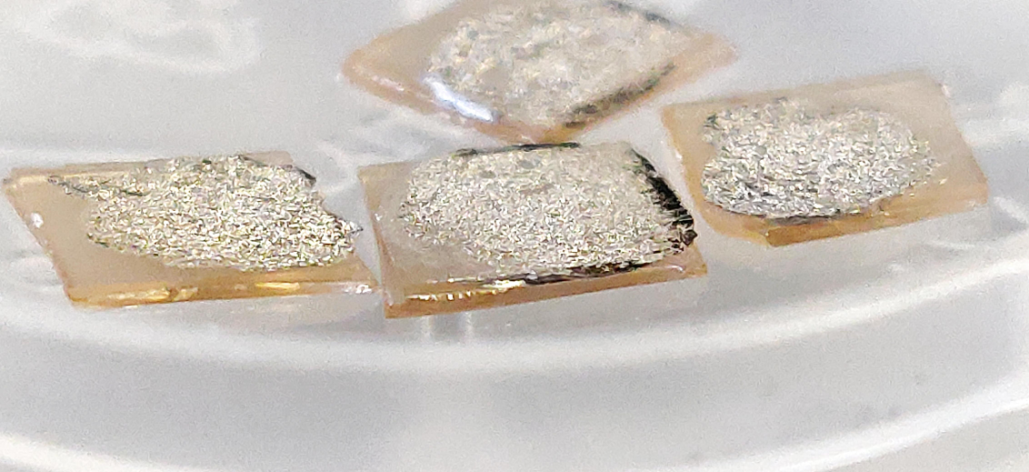
\includegraphics[width=\textwidth]{figs/4-Raman/CINTSamples.png}
        \caption{}
        \label{fig:Raman:CINTSamplesFacedown}
    \end{subfigure}
    \hfill
    \begin{subfigure}[b]{0.49\textwidth}
        \centering
        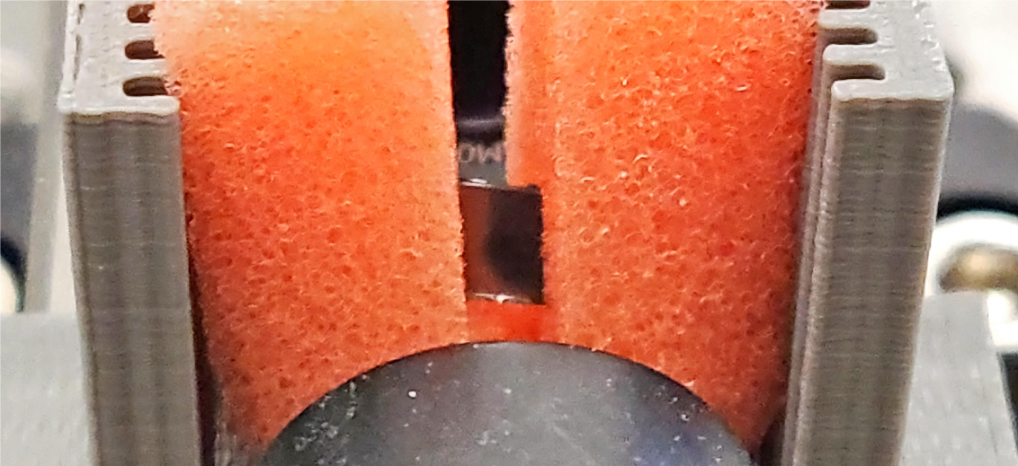
\includegraphics[width=\textwidth]{figs/4-Raman/TeCINTinFoam.png}
        \caption{}
        \label{fig:Raman:TeCINTinFoam}
    \end{subfigure}
    \caption{(\ref{fig:Raman:CINTSamplesFacedown}) Photograph of sapphire substrates primed with \SI{20}{\nano\meter} \ce{Se} adhesion layer. Critical surface is layed face down in curved-bottom protective container. (\ref{fig:Raman:TeCINTinFoam}) \SI{500}{\nano\meter} \ce{Te} thin film sample secured in beam path of \acl{CoBS}. \ce{Te} is deposited ontop of the \SI{20}{\nano\meter} \ce{Se} adhesion layer for ablation prevention.}
    \label{fig:Raman:CINTSamples}
\end{figure}

\section{Fiber-Chip-Fiber Waveguide Optical Alignment}
\label{Raman:Appendix:sec:WaveguideAlignment}

\begin{figure}[t]
  \centering
  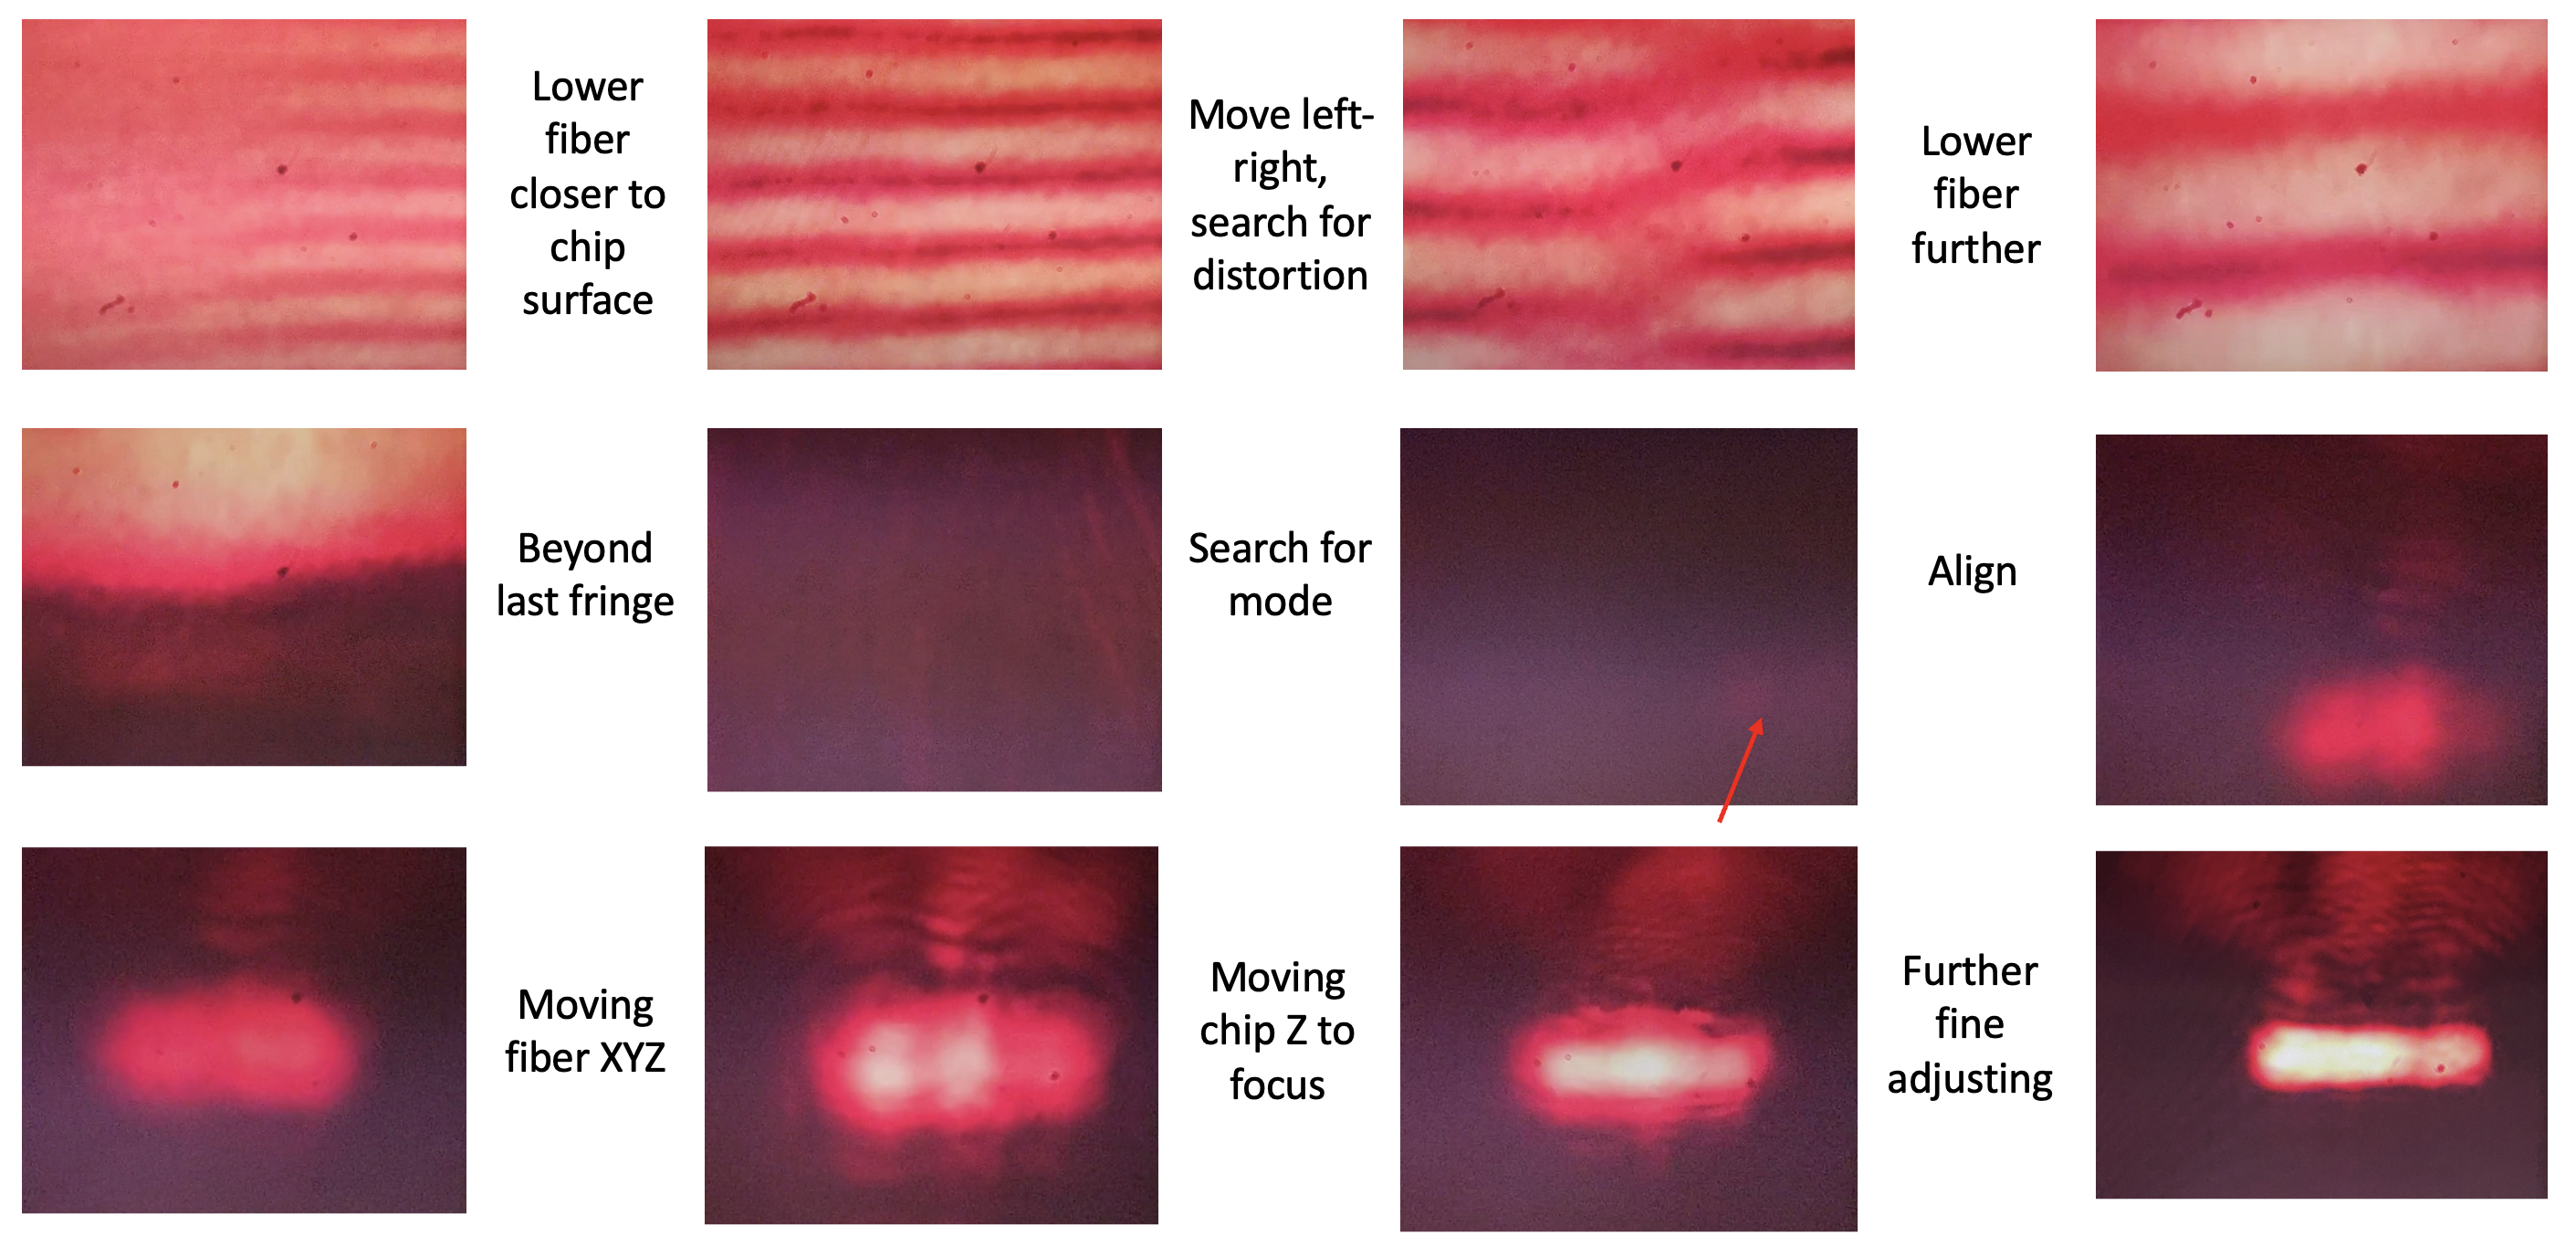
\includegraphics[width=\textwidth]{figs/4-Raman/WaveguideAlignmentCameraFringePattern.png}
  \caption{Step-by-step visuals from camera in process of aligning the input optical fiber to the chip waveguide, read from top left to bottom right.}
  \label{fig:Raman:WaveguideAlignmentCameraFringePattern}
\end{figure}

\section{Chip Waveguide Case Study~A: Thermal Effect on Brillouin Frequency Shift}
\label{Raman:Appendix:sec:CaseStudyAThermal}

freeze the lab

\section{Chip Waveguide Case Study~B: Pump-Probe Detuning Effect on Scattered Power}
\label{Raman:Appendix:sec:CaseStudyBDetuning}

P-Pr detuning


\chapter{Code and Data Availability}
\label{appendix:CodeandDataAvailability}
\acresetall

%\section{Python Script for CoBS Data Collection}

%\lstinputlisting[language=Python]{Code/CoBSPythonScript.py}

%\clearpage

\section{Plotting Data In Go}

Data plots presented in this dissertation were generated using custom programs written by the author in Golang or Python. The source code for these program, as well as all data collected and plots generated in support of the work presented in this dissertation, are publicly available on GitHub via the following link:

\hfill

\begin{center}
  \url{https://github.com/HamletTheHamster/Plotting-Data-in-Go}
\end{center}

\hfill

A video visualizing the evolution of data collection and development of functionality of the plotting program is available on YouTube:

\hfill

\begin{center}
  \url{https://www.youtube.com/watch?v=PdoWVoJx2Vg}
\end{center}

%\lstinputlisting[language=Go]{Code/plot.go}

\cleardoublepage


%%%%%%%%%%%%%%%%%%% REFERENCES %%%%%%%%%%%%%%%%%%%%%%%%%%%%%%%%%%%%%%%%%%%

%\singlespacing
\phantomsection
\addcontentsline{toc}{chapter}{References}
\renewcommand{\bibname}{References}
\bibliography{references.bib}

%%%%%%%%%%%%%%%%%%%%%%%%%%%%%%%%%%%%%%%%%%%%%%%%%%%%%%%%%%%%%%%%%%%%%%%%%%
\end{document}
